\documentclass[a4paper, 12pt, twoside, final, book, russian, fittopage, cyremdash]{ncc}
\usepackage[a4paper]{geometry}
\geometry{verbose, tmargin=3cm, bmargin=3cm, lmargin=2cm, rmargin=1.5cm, headheight=1cm, headsep=1cm, footskip=1.5cm}
\usepackage[T2A]{fontenc}
\usepackage[utf8]{inputenc}
\usepackage{wrapfig}
\usepackage[section]{placeins}
\usepackage{booktabs}
\usepackage{longtable}
\usepackage{hyperref}
\usepackage{xspace}
\usepackage[headings]{ncchdr}
\usepackage{ncccomma}
\usepackage{desclist}
\usepackage{indentfirst}
\usepackage{upgreek}
\usepackage{marvosym}
\usepackage{multirow}
\usepackage{amsfonts}
\usepackage{enumerate}
\usepackage{rotating}
\usepackage{array}
\usepackage{graphicx}
\usepackage[font=small]{caption}
\usepackage{xfrac}
\usepackage{multicol}
\usepackage{balance}
\usepackage{fixltx2e}


%\usepackage{showframe}

%\usepackage[warn]{mathtext}
%\usepackage[russian]{babel}
%\usepackage{misccorr}
%\usepackage{epigraph}
%\usepackage{quotchap}
%\usepackage[shortcuts, cyremdash]{extdash}
%\usepackage{appendix}
%\usepackage{cmap}
%\usepackage[texindy]{imakeidx}
%\usepackage{svg}
%\usepackage{amsmath}
%\usepackage[split]{splitidx}

\makeindex

% висячие и другие строки

\clubpenalty=10000
\widowpenalty=10000

\righthyphenmin=2 % разрешаем переносить два последних символа

\renewcommand{\bfdefault}{b} % плотный жирный

\newcommand{\mcyr}[1]{\ensuremath{\text{\textit{#1}}}}
\newcommand{\cidx}[2]{\ensuremath{#1_{\mcyr{#2}}}}
\newcommand{\lkvl}{\ensuremath{\cidx{L}{КВЛ}}\xspace}
\newcommand{\bkvl}{\ensuremath{\cidx{B}{КВЛ}}\xspace}
\newcommand{\tsr}{\ensuremath{\cidx{T}{ср}}\xspace}
\newcommand{\ve}[1]{\ensuremath{\mathbf{#1}}\xspace}
\newcommand{\gammaV}{\ensuremath{\ve{\gamma V}}\xspace}
\newcommand{\vidx}[2]{\ensuremath{\cidx{\ve #1}{#2}}\xspace}
\newcommand{\gr}{\ensuremath{\,^\circ}\xspace}
\newcommand{\grC}{\ensuremath{\,^{\circ}C}\xspace}
\newcommand{\midelsign}{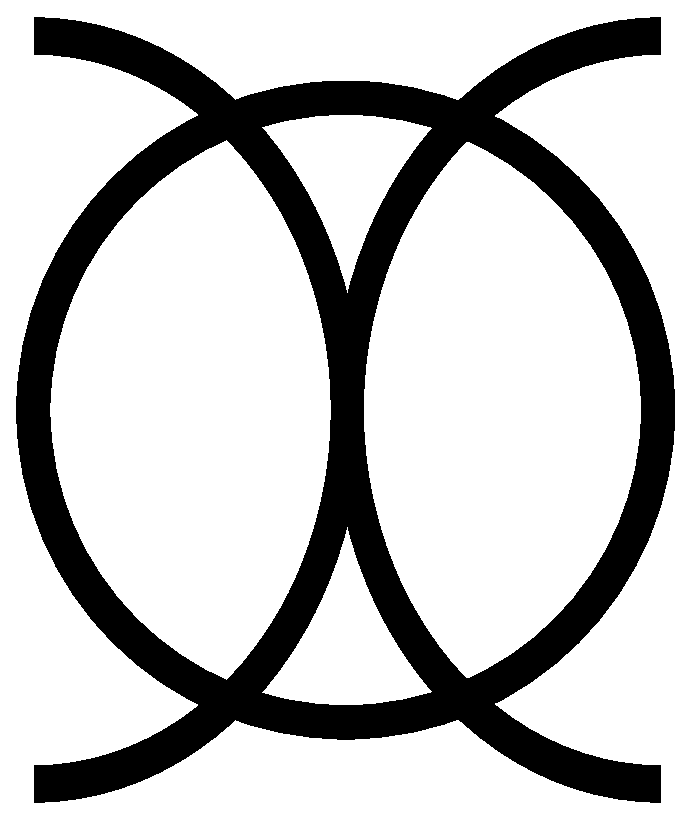
\includegraphics[scale=0.035]{midel_sign_vec.eps}\xspace}
\newcommand{\otdo}{\,\ensuremath{\div}\,}
\newcommand{\motdo}{\div}
\newcommand{\ris}[1]{\ref{fig:#1}}
\newcommand{\Renum}{\ensuremath{\mathrm {Re}}}
\newcommand{\msq}{~м\ensuremath{^2}\xspace}
\newcommand{\gmsq}{~г/м$^2$\xspace}
\newcommand{\kgmsq}{~кг/м$^2$\xspace}
\newcommand{\coursespelengs}[1]{\ensuremath{\text{\textit{#1}}}\xspace}
\newcommand{\IK}{\coursespelengs{ИК}}
\newcommand{\IP}{\coursespelengs{ИП}}
\newcommand{\OIP}{\coursespelengs{ОИП}}
\newcommand{\KU}{\coursespelengs{КУ}}
\newcommand{\MK}{\coursespelengs{МК}}
\newcommand{\OP}{\coursespelengs{ОП}}
\newcommand{\OMP}{\coursespelengs{ОМП}}
\newcommand{\Klb}{\ensuremath{\text{\textit{К}}_{\text{\textit{лев.борта}}}}\xspace}
\newcommand{\Kpb}{\ensuremath{\text{\textit{К}}_{\text{\textit{пр.борта}}}}\xspace}
\newcommand{\KK}{\coursespelengs{КК}}
\newcommand{\KP}{\coursespelengs{КП}}
\newcommand{\OKP}{\coursespelengs{ОКП}}
\newcommand{\MP}{\coursespelengs{МП}}
\newcommand{\PU}{\mcyr{ПУ}\xspace}
\newcommand{\PUb}{\ensuremath{\mcyr{ПУ}_\beta}\xspace}
\newcommand{\AP}{\cidx{A}{П}\xspace}
\newcommand{\Ost}{\ensuremath{{O^{st}}}\xspace}
\newcommand{\tauAries}{\ensuremath{\uptau^{\text{\Aries}}}\xspace}
\newcommand{\tmin}{\ensuremath{^\text{м}}\xspace}
\newcommand{\thr}{\ensuremath{^\text{ч}}\xspace}
\newcommand{\tsec}{\ensuremath{^\text{с}}\xspace}
\newcommand{\TSun}{\ensuremath{T^{\text{\Sun}}}}
\newcommand{\tSun}{\ensuremath{t^{\text{\Sun}}}}
\newcommand{\TNo}{\ensuremath{T_{\text{\No}}}\xspace}
\newcommand{\mathNo}{\text{\No}}
\newcommand{\hhmm}[2]{\ensuremath{#1\thr~#2\tmin}}
\newcommand{\hhmmss}[3]{\ensuremath{#1\thr~#2\tmin~#3\tsec}}
\newcommand{\Tgr}{\cidx{T}{ГР}\xspace}
\newcommand{\ppp}{\ensuremath{\text{п.}}}

\newcolumntype{M}{>{\centering\arraybackslash}m{\dimexpr.25\linewidth-2\tabcolsep}}

\graphicspath{{pics/}}

\begin{document}

\frontmatter

\author{\LARGE Составитель: Е.\=,П.~Леонтьев}
\title{Школа яхтенного капитана}
\setyear{1983}
\titlefoot{\theyear}
\maketitle

{\small \tableofcontents}
{\small \listoffigures}
{\small \listoftables}

\mainmatter

\part{Основы теории и устройство крейсерских яхт}

\chapter{Элементы теории парусной яхты}

\section{Требования, предъявляемые к парусной яхте.}

К уровню комфорта и оборудования на борту парусных яхт, в частности крейсерско\-/гоночных классов, предъявляются известные требования в соответствии с их назначением. Однако самый высокий уровень комфорта, самые совершенные приспособления для настройки парусов, самые современные электронные приборы для управления яхтой окажутся бесполезными, если она не будет обладать мореходными качествами, которые гарантируют безопасность плавания при условиях, определенных районом плавания и назначением яхты.

Яхта должна принимать определенную нагрузку, сохраняя достаточную высоту надводного борта, чтобы не быть залитой на волне. Она должна противостоять давлению ветра на паруса, чтобы не быть опрокинутой внезапно налетевшим шквалом. От яхты требуется хорошая маневренность в тесной гавани, и послушность рулю на штормовой волне. Она должна поддерживать, возможно, более высокую скорость при любых условиях и быть способной идти круто к ветру. Все это и составляет важнейшие мореходные качества: плавучесть, непотопляемость, остойчивость, ходкость, управляемость, поведение при волнении, способность нести паруса.

Изучение этих качеств является предметом специальной науки \--- теории корабля. Эта наука определяет также элементы, которые составляют отдельные мореходные качества и которые позволяют оценивать их количественно. Наконец, теория корабля устанавливает связь между формой корпуса судна и характеристиками его мореходных качеств.

В настоящей главе приводятся важнейшие элементы теории корабля в приложении к парусной яхте средних размерений в объеме, необходимом капитану при выходе в плавание.

\section{Характеристики формы корпуса яхты}

Основными характеристиками корпуса яхты являются его главные размерения и теоретический чертеж, дающий представление об обводах корпуса.

Главными размерениями яхты являются её длина, ширина, высота борта и осадка (рис.~\ris{1}). Знание этих величин необходимо для решения некоторых задач (плавание на мелководье, швартовка и т.\=,д.). Различают несколько значений каждого из этих размерений.

\begin{figure*}[htb]
   \centering
   \includegraphics[scale=1.3]{0001P.pdf}
   \caption{Главные размерения яхты}
   \label{fig:1}
\end{figure*}

\begin{description}
\item [Длина наибольшая\index{Длина наибольшая}] (в проектной документации судов она обозначается $L$) \--- расстояние по горизонтали, измеренное между крайними точками по обшивке судна.
\item [Длина по конструктивной ватерлинии\index{Длина по конструктивной ватерлинии} (\textit{КВЛ})] (\lkvl) \--- расстояние между крайними точками корпуса, измеренное по зеркалу воды при полной нагрузке судна либо при другой характерной нагрузке, например в состоянии обмера (см.~гл.~\ref{chap:4}).
\item [Ширина наибольшая\index{Ширина наибольшая}] ($B$) \--- измеряется в самом широком месте судна.
\item [Ширина по КВЛ\index{Ширина по конструктивной ватерлинии}] (\bkvl) \--- наибольшая ширина, измеренная в плоскости ватерлинии.
\item [Высота надводного борта\index{Высота надводного борта}] ($F$) \--- измеряется от ватерлинии до верхней кромки палубного настила у борта. Различают минимальный надводный борт \cidx{F}{М}, надводный борт в носу \cidx{F}{А} (измеряется по отвесу, опущенному из самой крайней точки форштевня) и надводный борт в корме \cidx{F}{К} (по отвесу, опущенному из крайней кормовой точки пересечения линии палубы с поверхностью транца).
\item [Осадка средняя\index{Осадка средняя}] (\tsr) \--- углубление судна, измеренное в средней части \--- на миделе \--- от ватерлинии до нижней кромки фальшкиля. На яхтах с длинной килевой линией измеряют еще максимальную осадку \--- от ватерлинии до самой нижней точки киля, обычно расположенной вблизи пятки руля.
\item [Полная высота борта на миделе\index{Полная высота борта на миделе}] ($H$) измеряется от верхней плоскости балластного фальшкиля до верхней кромки палубного настила у борта. Вместе с $L$ и $B$ высота борта используется в правилах постройки и классификации яхт в качестве параметра для назначения размеров поперечного сечения деталей набора корпуса, элементов якорного устройства и т.\=,п. 
\end{description}

Кроме главных размерений корпуса существуют еще габаритные размеры, например длина вместе с бушпритом, высота от нижней точки киля до верхней точки надстройки, ширина вместе с выступающими снаружи обшивки буртиками или привальным брусьями и т.\=,п.

Главные размерения яхты определяются из условий обеспечения требуемых мореходных качеств, внутреннего расположения жилых и служебных помещений, часто с целью получить определенный гоночный балл или класс. Они являются одними из основных количественных элементов, характеризующих эксплуатационные качества судна \--- его мореходность, вместимость и обитаемость.

Кроме абсолютных цифр судостроители и моряки часто оперируют безразмерными характеристиками \--- соотношениями главных размерений. Наиболее употребительными являются следующие.

\begin{description}
\item [Отношение длины по ватерлинии к ширине\index{Отношение длины по ватерлинии к ширине}] $\lkvl / \bkvl$ \--- характеризует ходкость судна (чем больше $ \lkvl / \bkvl$, тем легче на ходу, быстроходнее судно) и остойчивость (чем меньше $ \lkvl / \bkvl$, тем остойчивее яхта). У современных крейсерско-гоночных яхт, построенных по правилам IOR, $L/B = 2,5 \motdo 5,0$, у крейсерских швертботов $L/B = 2,8 \motdo 3,8$. 
\item [Отношение ширины по КВЛ к осадке\index{Отношение ширины по КВЛ к осадке}] $\bkvl / \tsr$ \--- характеризует ходкость, остойчивость и мореходность. Чем больше $\bkvl / \tsr$, тем остойчивее судно, однако его способность сохранять скорость при волнении оказывается ниже, чем у более узкой и глубокосидящей яхты. Яхты с классическими обводами корпусов имели $\bkvl / \tsr = 1,2 \motdo 1,6$; у современных крейсерско\-/гоночных яхт $\bkvl / \tsr = 1,8$. Для современных килевых яхт с выраженным плавниковым килем более характерно отношение $\bkvl / \cidx{T}{к}$, т.\=,е. ширины по КВЛ к осадке корпуса (без киля). 
\item [Отношение наибольшей длины к высоте борта\index{Отношение наибольшей длины к высоте борта}] $L/H$ \--- характеризует прочность и жесткость корпуса. Чем отношение меньше, тем большей продольной жесткостью обладает корпус, тем меньше он деформируется на волне и от тяги штагов. 
\end{description}

Теоретический чертеж яхты представляет сложную криволинейную наружную поверхность корпуса в виде проекций на три взаимно перпендикулярные плоскости. На этих проекциях изображаются следы пересечения наружной обшивки с секущими плоскостями, положение которых определяется в соответствии с установившимися в судостроении правилами. Три плоскости \--- диаметральная, основная и плоскость мидель-шпангоута являются базовыми плоскостями для построения теоретического чертежа и для постройки судна; они используются в качестве координатных плоскостей, от которых отсчитывают все размеры при последующей модернизации яхты.

\begin{description}
\item [Диаметральная плоскость\index{Диаметральная плоскость}] (\textit{ДП}) \--- вертикальная продольная плоскость симметрии, разделяющая корпус яхты на правую и левую половины. 
\item [Основная плоскость\index{Основная плоскость}] (\textit{ОП}) \--- горизонтальная плоскость, проходящая через самую нижнюю точку киля. Линия пересечения основной плоскости с \textit{ДП} называется основной линией (\textit{ОЛ}). 
\item [Плоскость мидель-шпангоута\index{Плоскость мидель-шпангоута}] (\textbf{миделя}\index{мидель}) \--- вертикальная поперечная плоскость, проходящая посередине длины яхты по КВЛ. Эту плоскость обозначают значком миделя \--- \midelsign. При оценке формы корпуса принято считать миделем самый большой по площади погруженной части шпангоут. 
\end{description}

Три проекции теоретического чертежа получаются сечением корпуса плоскостями, параллельными перечисленным трем базовым плоскостям. Боковая проекция (\textbf{<<бок>>}) образуется в результате сечения корпуса равноотстоящими друг от друга плоскостями, параллельными \textit{ДП}. Показанные на ней кривые линии сечений называются \textbf{батоксами}. Аналогичным образом получаются две другие проекции \--- \textbf{<<полуширота>>} и \textbf{<<корпус>>}. Первая образуется сечениями корпуса плоскостями, параллельными \textit{ОП} \--- \textbf{ватерлиниями}, вторая \--- сечением корпуса плоскостями, параллельными миделю \--- \textbf{шпангоутами}. На <<боку>> и <<полушироте>> шпангоуты изображаются в виде прямых линий; на <<корпусе>> они криволинейные. Ватерлинии выглядят в виде прямых на <<боку>> и <<корпусе>>, а батоксы \--- на <<полушироте>> и <<корпусе>> (рис.~\ris{2}). Прямые линии на каждой проекции образуют сетку теоретического чертежа.

\begin{figure*}[htb]
   \centering
   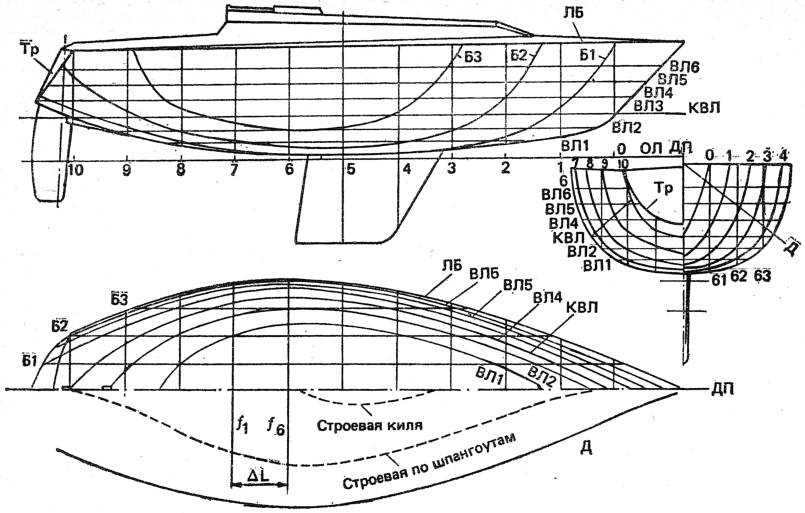
\includegraphics[scale=1.3]{0002P.pdf}
   \caption{Теоретический чертеж яхты <<Симфония>> (конструктор Филипп Брайан, Франция)}
   \label{fig:2}
   \centering{}
   \small  
   Длина наибольшая \--- 9,5~м; ширина наибольшая \--- 3,25~м; надводный борт минимальный \--- 1,02~м; осадка \--- 1,88~м; водоизмещение полное \--- 5,14~т. 1\==10 \--- шпангоуты, Тр \--- транец, ЛБ \--- линия борта, Б1\==Б3 \--- батоксы, ВЛ1\==ВЛ6 \--- ватерлинии, Д \--- диагональ (рыбина).
\end{figure*}

На теоретическом чертеже кроме упомянутых линий батоксов, шпангоутов и ватерлиний изображают очертания плавниковых килей, рулей, транца, фальшборта и т.\=,п. Так как корпус симметричен относительно \textit{ДП}, то на полушироте изображают ватерлинии только левого борта; на проекции <<Бок>> по правую сторону от линии \textit{ДП} вычерчивают обводы носовых шпангоутов, а по левую \--- обводы кормовых.

Все линии теоретического чертежа должны быть согласованы. Это значит, что любая точка на поверхности корпуса должна отстоять на равных расстояниях, например от \textit{ДП} на всех трех проекциях. При согласовании линий конструктор обычно проверяет положение точек пересечения кривых линий с прямыми линиями сетки. Для дополнительного согласования обводов корпуса на теоретическом чертеже проводят рыбины или диагонали \--- следы сечения корпуса продольными, наклонными к \textit{ДП} плоскостями, проведенными через характерные точки на проекции <<корпус>> \--- скулу, вогнутость при киле и т.\=,п. Диагонали проводятся только на <<корпусе>>, в виде прямых линий, и на полушироте вниз от \textit{ДП}, где они имеют вид плавных кривых линий.

Опытному глазу каждая из линий теоретического чертежа может многое сказать о качествах судна. Например, плавные стройные ватерлинии с острым входом в носу и не слишком крутой кривизной в корме благоприятны для хорошего обтекания корпуса водой, как и диагонали аналогичного вида. Батоксы с плавным и пологим \--- под углом $15 \motdo 20\gr$ к \textit{КВЛ} выходом над ватерлинией также важны для плавного, без завихрений, обтекания корпуса. Шпангоуты с явно выраженной скулой и переходом днища в борта по малому радиусу свидетельствуют о высокой начальной остойчивости яхты. В носовой части V-образные шпангоуты с острой вершиной при киле и плавным расширением к палубе важны для сохранения скорости на взволнованном море и незаливаемости палубы. 

Существенное влияние на обводы корпуса оказывают \textbf{Правила обмера}, по которым строится яхта. Так, в 70-х годах в результате введенного в правила обмера IOR, замера глубины трюма (расстояний от \textit{КВЛ} до внутренней поверхности обшивки) на миделе в трех местах по ширине яхты появились суда с трапециевидными шпангоутами. Эти же Правила дали жизнь принципиально новым обводам корпусов \--- с короткими свесами оконечностей, <<обратным>> наклоном транца, высоким надводным бортом и плавниковым килем, которые значительно отличаются от классических яхтенных обводов, господствовавших до конца 60-х годов.

Важнейшей характеристикой яхты является её \textbf{объемное водоизмещение} $V$, т.\=,е. объем воды, вытесняемый яхтой при её погружении по \textit{КВЛ}. Объемное водоизмещение яхты вместе с её главными размерениями позволяет судить о величине судна, его вместимости и потенциальных мореходных качествах. При сравнении яхт часто пользуются безразмерной характеристикой \--- \textbf{коэффициентом полноты водоизмещения} или \textbf{коэффициентом общей полноты} $\delta$, связывающим линейные размеры корпуса с его погруженным объемом. Этот коэффициент определяется как отношение объемного водоизмещения к объему параллелепипеда, имеющего стороны, равные \lkvl, \bkvl и \tsr (рис.~\ris{3}): 

\begin{equation}
\delta = \frac{V}{(\lkvl \cdot \bkvl \cdot  \tsr)}
\end{equation}

\begin{figure}[htb]
   \centering
   \includegraphics[scale=1.1]{0003P.pdf}
   \caption{Коэффициенты полноты}
   \label{fig:3}
   \centering{}\small $\delta$ \--- водоизмещения; $\alpha$ \--- ватерлинии; $\varphi$ \--- продольной полноты; $\beta$ \--- полноты мидель-шпангоута
\end{figure}

Чем меньше коэффициент общей полноты, тем более острые обводы имеет яхта, тем она быстроходнее. С другой стороны, при уменьшении $\delta$ соответственно уменьшается и полезный объем корпуса ниже ватерлинии, что вызывает необходимость для размещения кают достаточной высоты увеличивать высоту борта или делать более высокие надстройки. Парусные яхты относят к наименее полным судам. Коэффициент общей полноты для крейсерско-гоночных яхт составляет $\delta = 0,15 \motdo 0,22$, для крейсерских швертботов $\delta = 0,26 \motdo 0,35$. Корпуса шхерных крейсеров имели $\delta = 0,12 \motdo 0,15$, в то время как для большинства грузовых коммерческих судов характерна величина $\delta = 0,82$.

К числу безразмерных коэффициентов, характеризующих форму корпуса яхты, относятся также \textbf{коэффициенты полноты площадей ватерлинии} $\alpha$ и \textbf{мидель-шпангоута} $\beta$. Первый представляет собой отношение площади ватерлинии $S$ к прямоугольнику со сторонами  \lkvl и \bkvl: 

\begin{equation}
  \alpha = \frac{S}{\lkvl \cdot \bkvl} \quad ;
\end{equation}

второй \--- отношение площади погруженной части миделя \midelsign к прямоугольнику, стороны которого равны \bkvl и \tsr: 

\begin{equation}
\beta =  \frac{\midelsign}{\bkvl \cdot \tsr}
\end{equation}

Коэффициент $\alpha$, равный для большинства крейсерских яхт 0,70\otdo 0,72, для швертботов 0,60\otdo 0,67, показывает, насколько заострена \textit{КВЛ} в оконечностях, и какую роль в начальной остойчивости яхты играет форма её корпуса. С увеличением полноты ватерлинии повышается остойчивость, но несколько ухудшается обтекаемость корпуса и его ходкость на волне, особенно при большой осадке.

\textbf{Коэффициент продольной полноты} (или \textbf{призматический}) $\varphi$, который представляет собой отношение объемного водоизмещения к объему призмы, имеющей основанием погруженную часть миделя, а высотой длину яхты по КВЛ служит для оценки сопротивления воды движению яхт: 

\begin{equation}
\varphi = \frac{V}{\midelsign \cdot \lkvl}
\end{equation}

Призматический коэффициент, характеризуя распределение погруженного объема корпуса по длине, оказывает существенное влияние на ту часть энергии ветра, которая затрачивается на преодоление волнового сопротивления корпуса. Оптимальная величина $\varphi$ зависит от того, на какую скорость рассчитывается яхта. Если речь идет об очень быстроходных судах, то $\varphi$ принимается близким к $\varphi \approx 0,62$. Для яхт проектируемых на слабые ветра, $\varphi = 0,52 \motdo 0,53$.

\section{Плавучесть, осадка и дифферент}

\textbf{Плавучесть} \--- способность судна держаться на плаву, имея заданную осадку при определенной нагрузке. Это качество должно сохраняться в любых обстоятельствах эксплуатации яхты. 

На погруженную в воду поверхность судна при его неподвижном состоянии в каждой точке действуют силы гидростатического давления воды, направленные перпендикулярно поверхности. Все эти силы можно привести к одной силе плавучести, направленной вверх и приложенной в центре тяжести погруженного объема \--- \textbf{центре величины}, \textit{ЦВ}. Согласно известному закону Архимеда, сила плавучести равна массе воды, вытесненной судном.

Кроме давления воды на корпус судна действуют силы тяжести, которые также могут быть приведены к одной равнодействующей силе $D$, направленной вниз и приложенной в \textbf{центре тяжести}, \textit{ЦТ} судна. Для того чтобы судно плавало в состоянии равновесия, необходимо, чтобы сила плавучести и сила тяжести были равны и располагались на одной вертикали: 

\begin{gather}
  D = \gamma \cdot V \,;\  \cidx{x}{д} = \cidx{x}{с}
\end{gather}

где $\gamma$ \--- плотность воды, $\mbox{т}/\mbox{м}^3$; $V$ \--- объемное водоизмещение, $\mbox{м}^3$; $D$ \--- масса судна или массовое водоизмещение, т; \cidx{x}{д} \--- отстояние центра тяжести, \textit{ЦТ}, от плоскости миделя, м; \cidx{x}{с} \--- отстояние центра величины, \textit{ЦВ} от плоскости миделя, м.

В зависимости от плотности воды, в которой плавает яхта, её объемное водоизмещение может изменяться, хотя масса судна остается постоянной. В пресной воде, плотность которой близка к единице, для поддержания судна определенной массы требуется больший погруженный объем V, чем в соленой воде, плотность которой колеблется от $\gamma = 1,010 \motdo 1,015 \, \mbox{т}/\mbox{м}^3$ в Балтийском море до $1,023 \motdo 1,028 \, \mbox{т}/\mbox{м}^3$ в океане. Изменение объемного водоизмещения при переходе яхты из пресной воды ($\gamma = 1,00$) в морскую и наоборот происходит за счет изменения осадки. Величина этого изменения невелика \--- менее 1\,\% осадки и на эксплуатационных качествах яхты практически не сказывается. Однако влияние солености на осадку следует учитывать при обмере яхты и вычислении её гоночного балла. 

Знание главных размерений яхты и её коэффициентов полноты позволяет капитану выполнять некоторые элементарные расчеты приближенных значений водоизмещения, изменения осадки при приеме груза относительно небольшой величины. 

Водоизмещение:
\begin{equation}
D = \gamma \cdot \delta \cdot \lkvl \cdot \bkvl \cdot \tsr, \mbox{т.} 
\end{equation}

Груз, изменяющий осадку на 1 см:

\begin{equation}
  p = 0,01 \cdot \gamma \cdot \alpha \cdot \lkvl \cdot \bkvl, \mbox{т.}
\end{equation}

\begin{table*}[htb]
  \centering{}
  \begin{tabular}{p{0.5\textwidth}|c}
    \toprule
    Наименование раздела массовой нагрузки & Массовое водоизмещение, \,\% \\
    \midrule
    Корпус & 30--43 \\
    \midrule
    Фальшкиль & 30--45 \\
    \midrule
    Дельные вещи в корпусе и на палубе & 2--4,5 \\
    \midrule
    Оборудование помещений & 3--7 \\
    \midrule
    Рангоут, такелаж и паруса & 4--7 \\
    \midrule
    Двигатель с трубопроводами и электрооборудованием & 0--7 \\ 
    \midrule
    Системы с трубопроводами и цистернами & 2--4 \\
    \midrule
    Полезная нагрузка: экипаж с багажом, запасы пресной воды, провизии и топлива & 6--8 \\
    \bottomrule
    Массовое водоизмещение & $D = 100\,\%$ \\
  \end{tabular}
  \caption{Примерное распределение массового водоимещения между разделами нагрузки для крейсерско-гоночных яхт длиной 10\--14 метров}
  \label{tab:1}
\end{table*}

Если при проектировании или постройке яхты окажется, что её масса превышает водоизмещение по \textit{КВЛ}, а \textit{ЦТ} смещен в нос или корму от \textit{ЦВ}, то при спуске на воду она погрузится глубже конструктивной ватерлинии и получит наклон \--- \textbf{дифферент} на нос или на корму. При продольном наклонении в воду погружается дополнительный объем корпуса в носу или корме и в ту же сторону смещается точка приложения равнодействующей сил плавучести (\textit{ЦВ}) до того момента, пока вновь не будет достигнуто условие плавания в состоянии равновесия т.\=,е. $\cidx{x}{д} = \cidx{x}{с}$.

И увеличение осадки, и дифферент нежелательны, так как обводы ватерлиний яхты могут существенно отличаться от тех, что были предусмотрены её посадкой по проектной \textit{КВЛ}. Чтобы этого не случилось, после выбора главных размерений конструктор должен хотя бы приблизительно оценить массу будущей яхты. Для этого выполняется предварительный расчет массовой нагрузки по основным разделам: корпус; дельные вещи и палубное оборудование; оборудование внутренних помещений; рангоут, такелаж и паруса; двигатель с трубопроводами, гребным валом и электрооборудованием; системы с трубопроводами, цистернами; полезная нагрузка \--- экипаж, запасы пресной воды и провизии топливо для двигателя, снабжение; балластный фальшкиль. Примерное соотношение этих составляющих массовой нагрузки дано в табл.~\ref{tab:1}, а сумма их должна быть равна массово водоизмещению яхты по \textit{КВЛ}.

Существенное влияние на дифферент яхты оказывают переменные массы \--- топливо и вода в цистернах, которые расходуются в течение плавания, а также экипаж, имеющий возможность перемещаться по яхте. Поэтому цистерны для жидкостей стараются располагать вблизи общего ЦТ яхты, а экипаж во время гонки рассредоточивать на палубе и в помещениях, не допуская его скопления в кормовом кокпите, где масса людей создает значительный дифферентующий момент на корму.

\section{Непотопляемость}

Способность судна оставаться на плаву и сохранять свои мореходные качества в случае получения пробоины в обшивке или затопления через палубные отверстия называется \textbf{непотопляемостью}. Это свойство в первую очередь определяется запасом плавучести судна \--- его надводным объемом от \textit{КВЛ} до палубы. Чем выше надводный борт, тем больше запас плавучести, тем большее количество воды может влиться внутрь яхты, прежде чем она затонет.

Непотопляемость безбалластных швертботов и небольших яхт обеспечить сравнительно несложно. Благодаря легкой конструкции корпуса разность между массой яхты и силой поддержания в аварийном состоянии невелика. Требуется лишь небольшой дополнительный запас плавучести в виде междудонного пространства, бортовых отсеков плавучести, герметичных отсеков в носу и корме, под кокпитом. Для большей надежности эти отсеки заполняют легким пенистым пластиком, не впитывающим воду. Объем отсеков плавучести или блоков пенопласта рассчитывают так, чтобы при заполнении водой яхта держалась на плаву с надводным бортом около 10\,см и по возможности на ровном киле. Чтобы она сохраняла свою способность сопротивляться крену и дифференту, отсеки плавучести размещают в оконечностях корпуса и по бортам. 

Обеспечить непотопляемость крупной яхты, снабженной фальшкилем массой 40\--50\,\% её водоизмещения и имеющей большой объем внутренних помещений, практически невозможно. В данном случае помогло бы деление корпуса поперечными водонепроницаемыми переборками на несколько отсеков. Однако глухие переборки создают большие неудобства для обитаемости яхт, а при устройстве дверей переборки теряют смысл. Поэтому даже на больших яхтах устанавливают две водонепроницаемые переборки \--- форпиковую (вблизи носового конца \textit{КВЛ}) и ахтерпиковую (в районе кокпита), ограничивающие доступ воды внутрь при получении пробоины в оконечностях. 

Опыт, однако, показывает, что в море от пробоин при столкновениях яхты гибнут сравнительно редко. Гораздо большую опасность представляет негерметичность закрытий палубных люков, разбитые иллюминаторы. Именно это стало причиной гибели пяти яхт в трагической Фастнетской гонке 1979\,г. у берегов Ирландии. На этих яхтах (так же как и еще на 98 из 234 участвовавших в гонке судов) причиной попадания больших масс воды внутрь корпуса были ненадежные закрытия входных люков в стенках рубок. Традиционные задвижные щитки выскакивали из своих пазов при опрокидывании яхт, оказывались смытыми за борт или затерявшимися внутри яхт.

Современная практика требует, чтобы яхта, положенная парусами на воду, не могла быть залита через открытые люки. Входные люки предписывается оборудовать дверцами на прочных петлях, открываемыми обязательно наружу. Все иллюминаторы и светлые люки должны снабжаться защитными щитками, которые в штормовых условиях устанавливаются снаружи. Все отверстия в корпусе для забора забортной воды или выпуска сточных вод, воды из системы охлаждения двигателя и т.\=,п. снабжаются надежными запорными вентилями и клапанами, а осушительная система должна иметь достаточную производительность.

Современная крейсерско-гоночная яхта обладает большой живучестью, т.\=,е. способностью оставаться при аварии на плаву и перемещаться в нужном направлении. В упомянутой Фастнетской гонке на гребнях крутых волн опрокинулось 77 яхт, многие из которых совершили полный оборот на 360\gr. Несмотря на повреждения и большие массы воды, попавшие внутрь яхт, большинство из них были приведены в порты-убежища своими экипажами. Экипажи шести яхт, посчитавшие положение критическим, покинули их на надувных спасательных плотах, которые в тех условиях оказались недостаточно надежными. В результате погибло семь человек. В то же время только две из покинутых шести яхт действительно утонули. Четыре судна, несмотря на жестокий шторм, остались на плаву и были впоследствии обнаружены в море и отбуксированы в гавани.

\section{Силы, действующие на корпус и паруса яхты}

\begin{figure}[htb]
  \centering\includegraphics[scale=0.9]{0004P.pdf}
  \caption{\centering{} Схема сил, действующих на корпус и паруса яхты}
  \label{fig:4}
\end{figure}

До сих пор мы рассматривали действие на яхту только двух сил \--- силы плавучести и силы веса, предполагая, что она находится в равновесии состоянии покоя. Но поскольку для движения вперед на яхте используются паруса, на судно действует сложная система сил. Схематически она представлена на рис.~\ris{4}, где рассматривается наиболее типичный случай движения яхты в бейдевинд.

При обтекании парусов воздушным потоком \--- ветром \--- на них создается результирующая \textbf{аэродинамическая сила} \textbf{А}, направленная примерно перпендикулярно поверхности паруса и приложенная в центре парусности (\textit{ЦП}) высоко над поверхностью воды. Согласно третьему закону механики, при установившемся движении тела по прямой каждой силе, приложенной к телу, в данном случае \--- к парусам, связанным с корпусом яхты через мачту, стоячий такелаж и шкоты, должна противодействовать равная ей по величине и противоположно направленная сила. На яхте \--- это результирующая \textbf{гидродинамическая сила} \textbf{Н}, приложенная к подводной части корпуса. Таким образом, между этими силами существует известное расстояние \--- плечо, вследствие чего образуется момент пары сил.

И аэро- и гидродинамическая силы оказываются ориентированными не в плоскости, а в пространстве, поэтому при изучении механики движения яхты рассматривают проекции этих сил на главные координатные плоскости. Имея в виду упомянутый третий закон Ньютона, выпишем попарно все составляющие аэродинамической силы и соответствующие им гидродинамические реакции (см. таб.~\ref{tab:1-1}).

\begin{table*}[htb]
  \begin{tabular}{c|p{0.3\textwidth}|c|p{0.3\textwidth}}
    \toprule
    \shortstack[c]{Сила\\Момент} & \shortstack[c]{Описание\\\ } & \shortstack[c]{Сила\\Момент} & \shortstack[c]{Описание\\\ } \\
    \midrule
    $\ve{A}$ & Проекция аэродинамической результирующей силы & 
    $\ve{H}$ & Проекция гидродинамической результирующей силы \\
    $\ve{T}$ & Сила тяги, движущая яхту вперед &
    $\ve{R}$ & Сила сопротивления воды движению яхты \\
    $\vidx{F}{Д}$ & Кренящая сила или сила дрейфа &
    $\vidx{R}{Д}$ & Боковая сила или сила сопротивления дрейфу \\
    $\vidx{F}{В}$ & Вертикальная (аэродинамическая) сила &
    $\vidx{H}{В}$ & Вертикальная гидродинамическая сила \\
    $\ve D$ & Сила веса яхты &
    $\gammaV$ & Сила плавучести \\
    $\ve{M}_D$ & Дифферентующий момент &
    $\ve{M}_Z$ & Момент сопротивления дифференту \\
    $\vidx{M}{КР}$ & Кренящий момент &
    $\vidx{M}{В}$ & Восстанавливающий момент \\
    $\vidx{M}{П}$ & Приводящий к ветру момент &
    $\vidx{M}{У}$ & Уваливающий момент \\
    \bottomrule
  \end{tabular}
  \caption{Составляющие аэродинамической силы и соответствующие им гидродинамические реакции}
  \label{tab:1-1}
\end{table*}

Для того чтобы яхта устойчиво шла по курсу, каждая пара сил и каждая пара моментов сил должны быть равны друг другу. Например, сила дрейфа \vidx{F}{Д}, и сила сопротивления дрейфу \vidx{R}{Д} создают кренящий момент  \vidx{M}{КР}, который должен быть уравновешен восстанавливающим моментом \vidx{M}{В} или моментом поперечной остойчивости. \vidx{M}{В} образуется благодаря действию сил веса \ve{D} и плавучести яхты \ve V, действующих на плече $l$. Эти же силы веса и плавучести образуют момент сопротивления дифференту или момент продольной остойчивости $\ve{M}_l$, равный по величине и противодействующий дифферентующему моменту $\ve M_D$. Слагаемыми последнего являются моменты пар сил $\ve T - \ve R$ и $\vidx{F}{В} - \vidx{H}{В}$. 

В приведенную схему действия сил существенные поправки вносит, особенно на легких яхтах, экипаж. Перемещаясь на наветренный борт или по длине яхты, экипаж своим весом эффективно откренивает судно или противодействует его дифференту на нос. В создании уваливающего момента  \vidx{M}{У} решающая роль принадлежит соответствующему отклонению руля.

Аэродинамическая боковая сила  \vidx{F}{Д}, кроме крена вызывает боковой снос \--- дрейф, поэтому яхта движется не строго по \textit{ДП}, а с небольшим углом дрейфа $\lambda$. Именно это обстоятельство обусловливает образование на киле яхты силы сопротивления дрейфу \vidx{R}{Д}, которая по своей природе аналогична подъемной силе, возникающей на крыле самолета, располагаемом под углом атаки к набегающему потоку. Аналогично крылу работает на курсе бейдевинд и парус, для которого углом атаки является угол между хордой паруса и направлением вымпельного ветра. Таким образом, в современной теории корабля парусная яхта рассматривается как симбиоз двух крыльев: корпуса, движущегося в воде, и паруса, на который воздействует вымпельный ветер.

\section{Остойчивость}

Как мы уже говорили, яхта подвержена действию сил и моментов сил, стремящихся наклонить её в поперечном и продольном направлениях. Способность судна противостоять действию этих сил и возвращаться в прямое положение после прекращения их действия называется \textbf{остойчивостью}. Наиболее важной для яхты является \textbf{поперечная остойчивость}.

\begin{figure}[htb]
   \centering
   \includegraphics[scale=1.1]{0005P.pdf}
   \caption{Остойчивость килевой яхты}
   \label{fig:5}
   \centering{}\small Плечо остойчивости $l = \cidx{l}{Ф} - \cidx{l}{В}$
\end{figure}

Когда яхта плавает без крена, то силы тяжести и плавучести, приложенные соответственно в \textit{ЦТ} и \textit{ЦВ}, действуют по одной вертикали. Если при крене экипаж либо другие составляющие массовой нагрузки не перемещаются, то при любом отклонении \textit{ЦТ} сохраняет свое первоначальное положение в \textit{ДП} (точка $G$ на рис.~\ris{5}), вращаясь вместе с судном. В то же время вследствие изменившейся формы подводной части корпуса \textit{ЦВ} смещается из точки $C_0$ в сторону накрененного борта до положения $C_1$. Благодаря этому возникает момент пары сил \ve D и \gammaV с плечом $l$, равным горизонтальному расстоянию между \textit{ЦТ} и новым \textit{ЦВ} яхты. Этот момент стремится возвратить яхту в прямое положение и потому называется \textbf{восстанавливающим}.

При крене ЦВ перемещается по кривой траектории $C_0C_1$, радиус кривизны $r$ которой называется \textbf{поперечным метацентрическим радиусом}, а соответствующий ему центр кривизны $M$ \--- \textbf{поперечным метацентром}. Величина радиуса $r$ и соответственно форма кривой $C_0C_1$ зависят от обводов корпуса. В общем случае при увеличении крена метацентрический радиус уменьшается, так как его величина пропорциональна четвертой степени ширины ватерлинии. 

Очевидно, что плечо восстанавливающего момента зависит от расстояния $GM$ \--- возвышения метацентра над центром тяжести: чем оно меньше, тем соответственно меньше при крене и плечо $l$. На самой начальной стадии наклона величины $GM$ или $h$ рассматривается судостроителями как мера остойчивости судна и называется \textbf{начальной поперечной метацентрической высотой}. Чем больше $h$, тем необходима большая кренящая сила, чтобы наклонить яхту на какой-либо определенный угол крена, тем остойчивее судно. На крейсерско\-/гоночных яхтах метацентрическая высота составляет обычно 0,75\otdo 1,2\,м; на крейсерских швертботах \--- 0,6\otdo 0,8\,м. 

По треугольнику $GMN$ легко установить, что восстанавливающее плечо: $l = G \cdot N = h \cdot \sin \Theta$

Восстанавливающий момент, учитывая равенство \gammaV и \ve D, равен:

\begin{equation}
  \cidx{M}{В} = D \cdot h \cdot \sin \Theta
\end{equation}

Таким образом, несмотря на то, что метацентрическая высота изменяется в довольно узких пределах для яхт различных размерений, величина восстанавливающего момента прямо пропорциональна водоизмещению яхты, следовательно, более тяжелое судно оказывается в состоянии выдержать кренящий момент большей величины.

Восстанавливающее плечо можно представить как разность двух расстояний (см. рис.~\ris{5}): \cidx{l}{Ф} \--- плеча остойчивости формы и \cidx{l}{В} \--- плеча остойчивости веса. Нетрудно установить физический смысл этих величин, так как \cidx{l}{В} определяется отклонением при крене линии действия силы веса от первоначального положения точно над $C_0$, а \cidx{l}{Ф} \--- смещением на подветренный борт центра величины погруженного объема корпуса. Рассматривая действие сил \ve D и \gammaV относительно $C_0$, можно заметить, что сила веса \ve D стремится накренить яхту еще больше, а сила \gammaV, наоборот \--- выпрямить судно. 

\begin{figure}[htb]
  \centering
  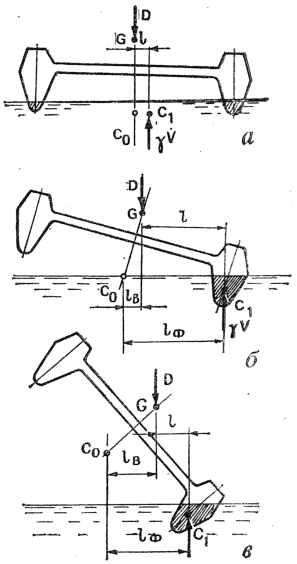
\includegraphics[scale=1.2]{0006P.pdf}
  \caption{Остойчивость катамарана}
  \label{fig:6}
  \small
  \centering{}
  \textit{а} \--- на малых углах крена; \textit{б} \--- в момент выхода наветренного корпуса из воды; \textit{в} \--- на больших углах крена
\end{figure}

По треугольнику $C_0GK$ можно найти, что $\cidx{l}{В} = G \cdot K = C_0 \cdot G \cdot \sin \Theta$, где $C_0 \cdot G$ \--- возвышение \textit{ЦТ} над \textit{ЦВ} в прямом положении яхты. Таким образом, для того чтобы уменьшить отрицательное действие сил веса, необходимо по возможности понизить \textit{ЦТ} яхты. В идеальном случае \textit{ЦТ} должен бы расположиться ниже \textit{ЦВ}, тогда плечо остойчивости веса становится положительным и масса яхты помогает ей сопротивляться действию кренящего момента. Однако только немногие яхты имеют такую характеристику: углубление \textit{ЦТ} ниже \textit{ЦВ} связано с применением очень тяжелого балласта, превышающего 60\,\% водоизмещения яхты, чрезмерным облегчением конструкции корпуса, рангоута и такелажа. Эффект, аналогичный снижению \textit{ЦТ}, дает перемещение экипажа на наветренный борт. Если речь идет о легком швертботе, то экипажу удается сместить общий \textit{ЦТ} настолько, что линия действия силы \ve D пересекается с \textit{ДП} значительно ниже \textit{ЦВ} и плечо остойчивости веса получается положительным.

У килевой яхты благодаря тяжелому балластному фальшкилю центр тяжести находится достаточно низко (чаще всего \--- под ватерлинией или слегка выше нее). Остойчивость яхты всегда положительная и достигает максимума при крене около 90\gr, когда яхта лежит парусами на воде. Разумеется, такой крен может быть достигнут только на яхте с надежно закрытыми отверстиями в палубе и с самоотливным кокпитом. Яхта с открытым кокпитом может быть залита водой при гораздо меньшем угле крена (яхта класса <<Дракон>>, например, при 52\gr) и пойти ко дну не успев выпрямиться.

У мореходных яхт положение неустойчивого равновесия наступает при крене около 130\gr, когда мачта уже находится под водой, будучи направленной, вниз под углом 40\gr к поверхности. При дальнейшем увеличении крена плечо остойчивости становится отрицательным, опрокидывающий момент способствует достижению второго положения неустойчивого равновесия при крене 180\gr (вверх килем), когда \textit{ЦТ} оказывается расположенным высоко над \textit{ЦВ} достаточно небольшой волны, чтобы судно приняло вновь нормальное положение \--- вниз килем. Известно немало случаев, когда яхты совершали полный оборот на 360\gr и сохраняли свои мореходные качества. 

Сравнивая остойчивость килевой яхты и швертбота, можно заметить, что главную роль в создании восстанавливающего момента у швертбота играет остойчивость формы, а у килевой яхты \--- остойчивость веса. Поэтому и существует столь заметная разница в обводах их корпусов: швертботы имеют широкие корпуса с $L/B = 2,6 \motdo 3,2$, со скулой малого радиуса и большой полнотой ватерлинии. В еще большей степени форма корпуса определяет остойчивость катамаранов, у которых объемное водоизмещение разделено поровну между двумя корпусами. Уже при небольшом крене водоизмещение между корпусами резко перераспределяется, увеличивая силу плавучести корпуса, погружающегося в воду (рис.~\ris{6}). Когда другой корпус выходит из воды (при крене 8\otdo 15\gr), плечо остойчивости достигает максимальной величины \--- оно немного меньше половины расстояния между \textit{ДП} корпусов. При дальнейшем увеличении крена катамаран ведет себя подобно швертботу, экипаж которого висит на трапеции. При крене 50\otdo 60\gr наступает момент неустойчивого равновесия, после чего остойчивость катамарана становится отрицательной.

\begin{figure*}[htb]
  \centering
  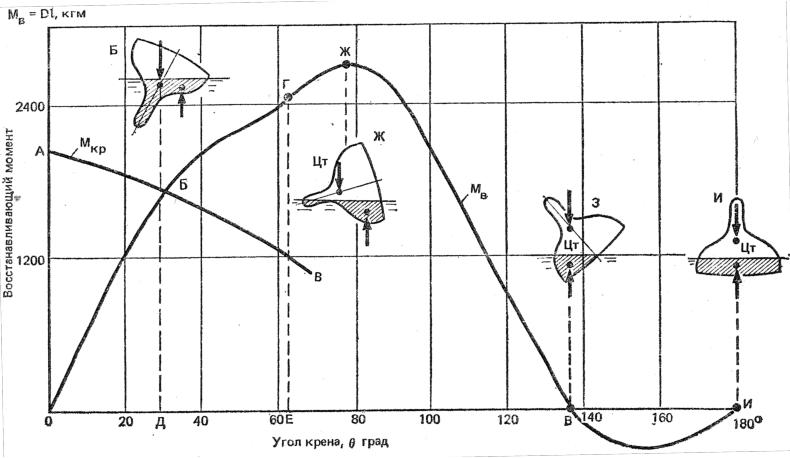
\includegraphics[scale=1.3]{0007P.pdf}
  \caption{Диаграмма статической остойчивости крейсерско-гоночной яхты}
  \label{fig:7}
\end{figure*}

\textbf{Диаграмма статической остойчивости}. Очевидно, что полной характеристикой остойчивости яхты может быть кривая изменения восстанавливающего момента \vidx{M}{В} в зависимости от угла крена $\Theta$ или диаграмма статической остойчивости (рис.~\ris{7}). На диаграмме хорошо различимы моменты максимума остойчивости (Ж) и предельного угла крена, при котором судно, будучи предоставлено само себе, опрокидывается (З \--- угол заката диаграммы статической остойчивости).

С помощью диаграммы капитан судна имеет возможность оценивать, например, способность яхты нести ту или, иную парусность при ветре определенной силы. Для этого на диаграмму остойчивости наносят кривые изменения кренящего момента \vidx{M}{КР} в зависимости от угла крена $\Theta$. Точка Б пересечения обеих кривых указывает на угол крена, который получит яхта при статическом, с плавным нарастанием действии ветра. На рис.~\ris{7} яхта получит крен, соответствующий точке Д, \--- около 29\gr. Для судов, имеющих явно выраженные нисходящие ветви диаграммы остойчивости (швертботов, компромиссов и катамаранов), плавание может, быть допущено только при углах крена, не превышающих точки максимума на диаграмме остойчивости. 

На практике экипажам яхт приходится нередко иметь дело с динамическим действием внешних сил, при котором кренящий момент достигает значительной величины в сравнительно короткий промежуток времени. Такое бывает при шквале или ударе волны в наветренную скулу. В этих случаях важна не только величина кренящего момента, но и кинетическая энергия, сообщаемая судну и поглощаемая работой восстанавливающего момента. 

На диаграмме статической остойчивости работа обоих моментов может быть представлена в виде площадей, заключенных между соответствующими кривыми и осями ординат. Условием равновесия яхты при динамическом воздействии внешних сил будет равенство площадей ОАБВЕ (работа \vidx{M}{КР}) и ОБГВЕ (работа \vidx{M}{В}). Учитывая, что площади ОБВЕ общие, можно рассматривать равенство площадей ОАБ и БГВ. На рис.~\ris{7} видно, что в случае динамического действия ветра угол крена (точка Е, около 62\gr) заметно превышает крен от ветра такой же силы при его статическом действии. 

По диаграмме статической остойчивости может быть определен \textbf{предельный динамический кренящий момент}, опрокидывающий швертбот или угрожающий безопасности яхты с открытым кокпитом. Очевидно, что действие восстанавливающего момента может рассматриваться только до угла заливания кокпита или до начальной точки снижения диаграммы статической остойчивости.

Принято считать, что килевые яхты, снабженные тяжелым балластом, практически неопрокидываемы. Однако в уже упоминавшейся Фастнетской гонке 1979\,г. 77 яхт были опрокинуты на угол крена более 90\gr, причем часть из них некоторое время (от 30 сек до 5 мин) оставалась на плаву вверх килем, а несколько яхт встали потом в нормальное положение через другой борт. Наиболее серьезными повреждениями при этом были потери мачт (на 12 яхтах), падение из своих гнезд аккумуляторов, тяжелых камбузных плит и другого оборудования. К нежелательным последствиям привело и попадание воды внутрь корпусов. Случилось это под динамическим воздействием крутой 9--10\-/метровой волны, профиль которой резко ломался при переходе из океана в мелководное Ирландское море, при ветре скоростью 25\otdo 30\,м/с.

\textbf{Факторы, влияющие на поперечную остойчивость}. Таким образом, мы можем сделать определенные выводы о влиянии различных элементов проекта яхты на её остойчивость. На малых углах крена главную роль в создании восстанавливающего момента играют ширина яхты и коэффициент полноты площади ватерлинии. Чем шире яхта и полнее её ватерлиния, тем дальше от \textit{ДП} смещается \textit{ЦВ} при крене судна, тем больше плечо остойчивости формы. Диаграмма статической остойчивости достаточно широкой яхты имеет более крутую восходящую ветвь, чем узкой, \--- до $\Theta = 60 \motdo 80gr$. 

Чем ниже расположен центр тяжести яхты, тем она остойчивее, причем влияние глубокой осадки и большого балласта сказывается практически по всей диаграмме остойчивости яхты. Занимаясь модернизацией яхты, полезно помнить простое правило: каждый килограмм под ватерлинией повышает остойчивость, а каждый килограмм над ватерлинией ухудшает её. Особенно ощутим для остойчивости тяжелый рангоут и такелаж.

При одинаковом расположении центра тяжести яхта с избыточным надводным бортом имеет и более высокую остойчивость на углах крена более 30\otdo 35\gr, когда на судне с нормальной высотой борта палуба начинает входить в воду. Высокобортная яхта имеет большую величину максимального восстанавливающего момента. Это качество присуще также яхтам, имеющим водонепроницаемые рубки достаточно большого объема. 

Особо следует остановиться на влиянии воды в трюме и жидкостей в цистернах. Дело не только в перемещении масс жидкостей в сторону накрененного борта; главную роль играет наличие свободной поверхности переливающейся жидкости, а именно \--- её момент инерции относительно продольной оси. Если, например, поверхность воды в трюме имеет длину $l$, а ширину $b$, то метацентрическая высота уменьшается на величину

\begin{equation}
  \Delta h = \frac{l \cdot b^3}{\ 12D\ }, \quad \text{м.}
\end{equation}

Особенно опасна вода в трюме, свободная поверхность которого имеет большую ширину. Поэтому при плавании в штормовых условиях воду из трюма нужно своевременно удалять.

Для уменьшения влияния свободной поверхности жидкостей в цистернах устанавливают продольные отбойные переборки, которые по ширине делят на несколько частей. В переборках делают отверстия для свободного перетекания жидкости.

\textbf{Поперечная остойчивость и ходкость яхты.} При увеличении крена сверх 10\otdo 12\gr сопротивление воды движению яхты заметно возрастает, что приводит к потере скорости. Поэтому важно, чтобы при усилении ветра яхта дольше могла нести эффективную парусность, не имея чрезмерного крена.Нередко даже на сравнительно крупных яхтах во время гонок экипаж располагается на наветренном борту, пытаясь уменьшить крен. 

Насколько эффективно перемещение груза (экипажа) на один борт, нетрудно представить по простейшей формуле, которая справедлива для небольших углов (в пределах 0\otdo 10\gr) крена:

\begin{equation}
  \vidx{M}{О} = \frac{D \cdot h}{57,3} \quad ,
\end{equation}

где: \vidx{M}{O} \--- момент, кренящий яхту на 1\gr; $D$ \--- водоизмещение яхты, т; $h$ \--- начальная поперечная метацентрическая высота, м. 

Зная массу перемещаемого груза и расстояние нового места расположения его от \textit{ДП}, можно определить кренящий момент, а разделив его на \vidx{M}{О}, получить угол крена в градусах. Например, если на яхте водоизмещением 7\,т при $h=1\,\text{м}$ пять человек расположатся у борта на расстоянии 1,5\,м от \textit{ДП}, то создаваемый ими кренящий момент придаст яхте крен в 4,5\gr (или уменьшит примерно на столько же крен на другой борт). 

\textit{Продольная остойчивость.} Физика явлений, происходящих при продольных наклонах яхты аналогична явлениям при крене, но продольная метацентрическая высота по величине сравнима с длиной яхты. Поэтому продольные наклоны, дифферент, обычно невелики и измеряются не в градусах, а по изменениям осадки носом и кормой. И, тем не менее, если из яхты выжимают все её возможности, нельзя не считаться с действием сил, дифферентующих яхту на нос и перемещающих центр величины, вперед (см. рис.~\ris{4}). Этому можно противодействовать, перемещая экипаж в кормовую часть палубы. 

Наибольшей величины дифферентующие на нос силы достигают при плавании в бакштаг; на этом курсе, особенно в сильный ветер, экипаж следует смещать, возможно, дальше в корму. На курсе бейдевинд дифферентующий момент невелик, и экипажу лучше всего располагаться близ миделя, откренивая судно. На фордевинде дифферентующий момент оказывается меньше, чем на бакштаге, особенно если яхта несет спинакер и блупер, дающие определенную подъемную силу.

У катамаранов величина продольной метацентрической высоты сравнима с поперечной, иногда меньше нее. Поэтому действие дифферентующего момента, практически незаметное на килевой яхте, может опрокинуть катамаран, таких же главных размерений. Статистика аварий отмечает случаи опрокидывания через нос на попутных курсах крейсерских катамаранов с высокой парусностью. 

\section{Сопротивление дрейфу}

Поперечная сила \vidx{F}{Д} (см. рис.~\ris{4}) не только кренит яхту, она вызывает боковой снос \--- \textbf{дрейф под ветер}. Сила дрейфа зависит от курса яхты относительно ветра. При плавании в крутой бейдевинд она втрое превышает силу тяги, движущую яхту вперед; на галфвинде обе силы примерно равны; в крутой бакштаг (истинный ветер около 135\gr относительно курса яхты) движущая сила оказывается в 2--3 раза больше силы дрейфа, а на чистом фордевинде сила дрейфа вовсе отсутствует. Следовательно, для того чтобы судно успешно продвигалось вперед курсом от бейдевинда до галфвинда, оно должно обладать достаточным боковым сопротивлением дрейфу, намного превышающим сопротивление воды движению яхты по курсу. 

Функцию создания силы сопротивления дрейфу у современных яхт выполняют в основном шверты, плавниковые кили и рули. 

Как мы уже говорили, непременным условием возникновения силы сопротивления дрейфу является движение яхты под небольшим углом к \textit{ДП} \--- углом дрейфа. Рассмотрим, что при этом происходит в потоке воды непосредственно у киля, который представляет собой крыло с поперечным сечением в виде тонкого симметричного аэродинамического профиля (рис.~\ris{8}).

\begin{figure*}[htb]
  \centering
  \includegraphics[scale=1.3]{0008P.pdf}
  \caption{Образование подъемной силы на крыле}
  \label{fig:8}
  \centering{}\small \textit{a} \--- обтекание профиля при $\alpha = 0$;
                     \textit{б}~и~\textit{в} \--- образование стартового вихря;
                     \textit{г} \--- отрыв стартового вихря;
                     \textit{д} \--- появление устойчивой циркуляции потока вокруг крыла;
                     \textit{е} \--- схема действующих сил при развитой циркуляции
\end{figure*}

Если угол дрейфа отсутствует (рис.~\ris{8},~\textit{а}), то поток воды, встречаясь с профилем киля в точке \textit{а}, разделяется на две части. В этой точке, называемой критической, скорость потока равна 0, давление максимальное, равное скоростному напору $(\rho \cdot v^2) / 2$, где: $\rho$ \--- массовая плотность воды (для пресной воды = 102 $\text{кгс}^2 / \text{м}^4$ ); $v$ \--- скорость движения яхты (м/с). 

И верхняя и нижняя части потока одновременно обтекают поверхности профиля и вновь встречаются в точке \textit{b} на выходящей кромке. Очевидно, что никакой силы, направленной поперек потока, на профиле возникнуть не может; будет действовать только одна сила сопротивления трения, обусловленная вязкостью воды. 

Если же профиль отклонить на некоторый угол атаки $\alpha$ (в случае яхтенного киля \--- угол дрейфа), то картина обтекания профиля изменится (рис.~\ris{8},~\textit{б}). Критическая точка $a$ переместится на нижнюю часть <<носика>> профиля. Путь, который должна пройти частица воды вдоль верхней поверхности профиля, удлинится, а точка $b_1$, где по условиям неразрывности потока должны были бы встретиться частицы, обтекающие верхнюю и нижнюю поверхности профиля, пройдя равный путь, оказывается на верхней поверхности. Однако при огибании острой выходящей кромки профиля нижняя часть потока срывается с кромки в виде вихря (рис.~\ris{8},~\textit{в} и \textit{г}). Этот вихрь, называемый стартовым, вращаясь против часовой стрелки, вызывает циркуляцию воды вокруг профиля в обратном направлении, т.\=,е. по часовой стрелке (рис.~\ris{8},~\textit{д}). Данное явление, вызванное силами вязкости, аналогично вращению большого зубчатого колеса (циркуляция), находящегося в зацеплении с малой ведущей шестерней (стартовый вихрь). 

После того как возникает циркуляция, стартовый вихрь срывается с выходящей кромки, точка $b_2$ перемещается ближе к этой кромке, вследствие чего здесь больше не существует разности скоростей, с которыми крыло покидают верхняя и нижняя части потока. Циркуляция же вокруг крыла становится причиной возникновения подъемной силы \ve Y, направленной поперек потока: у верхней поверхности крыла скорость частиц воды за счет циркуляции увеличивается, у нижней, встречаясь с частицами, вовлеченными в циркуляцию, \--- затормаживается. Соответственно у верхней поверхности давление понижается по сравнению с давлением в потоке перед крылом, а у нижней поверхности \--- повышается. Разность давлений и дает подъемную силу \ve Y. 

Кроме того, на профиль будет действовать \textbf{сила лобового (профильного) сопротивления} \ve X, возникающая вследствие трения воды о поверхность профиля и гидродинамического давления на его переднюю часть.

\begin{figure}[htb]
  \centering
  \includegraphics[scale=1.2]{0009P.pdf}
  \caption{Распределение давления по ширине симметричного аэродинамического профиля при угле атаки $\alpha = 7\gr$}
  \label{fig:9}
\end{figure}

На рис.~\ris{9} представлены результаты замера давления у поверхности симметричного профиля, сделанного в аэродинамической трубе. По оси ординат отложено значение коэффициента $C_P$, который представляет собой отношение избыточного давления (полное давление минус атмосферное) к скоростному напору $(\rho \cdot v^2) / 2$. На верхней стороне профиля давление отрицательное (разрежение), на нижней \--- положительное. Таким образом, подъемная сила, действующая на любой элемент профиля, складывается из действующих на него сил давления и разрежения, а в целом она пропорциональна площади, заключенной между кривыми распределения давления по хорде профиля (на рис.~\ris{9} заштриховано).

Данные, представленные на рис.~\ris{9}, позволяют сделать ряд важных выводов о работе яхтенного киля. Во-первых, главную роль в создании боковой силы играет разрежение, возникающее на поверхности плавника со стороны наветренного борта. Во-вторых, пик разрежения располагается вблизи входящей кромки киля. Соответственно точка приложения результирующей подъемной силы находится на передней трети хорды плавника. В целом же подъемная сила возрастает вплоть до угла атаки 15\otdo 18\gr, после чего внезапно падает.

Вследствие образования завихрения на стороне разрежения плавное обтекание крыла нарушается, разрежение падает и происходит срыв потока (это явление более подробно рассмотрено в гл.~\ref{chap:2} для парусов). Одновременно с увеличением угла атаки возрастает лобовое сопротивление \--- оно достигает максимума при $\alpha = 90\gr$.

Величина дрейфа современной яхты редко превышает 5\gr, так что срыв, потока с киля можно не опасаться. Однако критический угол атаки должен учитываться для яхтенных рулей, которые проектируются и работают также по принципу крыла. 

Рассмотрим основные параметры яхтенных килей, которые оказывают существенное влияние на их эффективность в создании силы сопротивлению дрейфу. В равной степени изложенное далее можно распространить и на рули с учетом того, что они работают со значительно большим углом атаки.

\textbf{Толщина и форма поперечного сечения киля.} Испытания симметричных аэродинамических профилей показали, что более толстые профили (с большей величиной отношения толщины сечения $t$ к его хорде $b$) дают большую подъемную силу. Их лобовое сопротивление выше, чем у профилей с меньшей относительной толщиной. Оптимальные результаты могут быть получены при $t/b = 0,09 \motdo 0,12$. Величина подъемной силы на таких профилях сравнительно мало зависит от скорости яхты, поэтому кили развивают достаточную силу сопротивления дрейфа и в слабый ветер. 

Существенное влияние на величину силы сопротивления дрейфу оказывает положение максимальной толщины профиля по длине хорды. Наиболее эффективными оказываются профили, у которых максимальная толщина расположена на расстоянии 40\otdo 50\,\% хорды от их <<носика>>. Для яхтенных рулей, работающих под большими углами атаки, используют профили с максимальной толщиной, расположенной несколько ближе к передней кромке, \--- до 30\,\% хорды.

Определенное влияние на эффективность киля оказывает форма, <<носика>> профиля \--- радиус округления входящей кромки. Если кромка слишком острая, то набегающий на киль поток получает здесь большое ускорение и срывается с профиля в виде вихрей. При этом происходит падение подъемной силы, особенно существенное при больших углах атаки. Поэтому подобное заострение входящей кромки недопустимо для рулей. 

\textbf{Аэродинамическое удлинение.} У концов крыла обнаруживается перетекание воды из области повышенного давления на спинку профиля. В результате с концов крыла срываются вихри, образующие две вихревые дорожки. На их поддержание затрачивается довольно значительная часть энергии, образуя так называемое \textbf{индуктивное сопротивление}. Кроме того, вследствие выравнивания давлений у концов крыла происходит местное падение подъемной силы, как это показано на эпюре распределения её по длине крыла на рис.~\ris{10}. 

\begin{figure*}[htb]
  \centering
  \includegraphics[scale=1.3]{0010P.pdf}
  \caption{Схема обтекания крыла конечного размаха}
  \label{fig:10}
  \centering
  \small
  \textit{1} \--- распределение подъемной силы по длине крыла;
  \textit{2} \--- циркуляция;
  \textit{3} \--- перетекание жидкости по концам крыла;
  \textit{4} \--- концевые вихри;
  \textit{5} \--- распределение вызванных скоросте по размаху крыла $L$
\end{figure*}

Чем короче длина крыла $L$ по отношению к его хорде $b$, т.\=,е. чем меньше его удлинение $L/b$, тем относительно больше потеря подъемной силы и тем больше индуктивное сопротивление. В аэродинамике принято оценивать удлинение крыла по формуле $\lambda = L^2/S$ (где $S$ \--- площадь крыла), которая может быть применена для крыльев и плавников любых очертаний. При прямоугольной форме аэродинамическое удлинение равно соотношению $\lambda = L / b$; для треугольного крыла $\lambda = 2 \cdot L / b$.
На рис.~\ris{10} показано крыло, составленное из двух трапециевидных плавниковых килей. На яхте киль крепится широким основанием к днищу, поэтому здесь перетекание воды на сторону разрежения отсутствует и под влиянием корпуса давления на обоих поверхностях выравнивается. Без этого влияния можно было бы считать аэродинамическое удлинение вдвое большим, чем отношение глубины киля к его осадке. На практике же это отношение, зависящее от размеров киля, обводов яхты и угла крена превышается только в 1,2\otdo 1,3 раза.

\begin{figure}[htb]
  \centering
  \includegraphics[scale=1.2]{0011P.pdf}
  \caption{Зависимость сопротивления дрейфу от удлинения киля и угла атаки}
  \label{fig:11}
\end{figure}

Влияние аэродинамического удлинения киля на величину развиваемой им силы сопротивления дрейфу \vidx{R}{Д} можно оценить по результатам испытаний плавника, имеющего профиль NACA 009 ($t/b = 9\,\%$) и площадь 0,37\msq (рис.~\ris{11}). Скорость потока соответствовала скорости движения яхты 3 узла (1,5\,м/с). Интерес представляет изменение силы сопротивления дрейфу при угле атаки 4\otdo 6\gr, что соответствует углу дрейфа яхты на курсе бейдевинд. Если принять силу \vidx{R}{Д} при удлинении $\lambda = 1$ за единицу (6,8 при $\alpha = 5\gr$), то при увеличении $\lambda$ до 2 сопротивление дрейфу увеличивается более чем в 1,5 раза (10,4\,кг), а при $\lambda = 3$ \--- ровно вдвое (13,6\,кг). Этот же график может служить для качественной оценки эффективности рулей различного удлинения, которые работают в области больших углов атаки.

Таким образом, увеличивая удлинение плавника киля, можно получить необходимую величину боковой силы \vidx{R}{Д} при меньшей площади киля и, следовательно, при меньшей площади смоченной поверхности и сопротивлении воды движению яхты. Удлинение килей на современных крейсерско\-/гоночных яхтах составляет в среднем $\lambda = 1 \motdo 3$. Перо руля, служащее не только для управления судном, но и являющееся составным элементом в создании сопротивления яхты, имеет еще большее удлинение, приближающееся к $\lambda = 4$. 

\textbf{Площадь и формы киля.} Чаще всего размеры киля определяют по статистическим данным, сравнивая проектируемую яхту с хорошо зарекомендовавшими себя судами. На современных крейсерско\-/гоночных яхтах с раздельным от киля рулем суммарная площадь киля и руля составляет от 4,5 до 6,5\,\% площади парусности яхты, а площадь руля \--- 20\otdo 40\,\% площади киля.

Для получения оптимального удлинения конструктор яхты стремится принять осадку наибольшей допускаемой по условиям плавания или правилами обмера. Чаще всего киль имеет вид трапеции с наклонной передней кромкой. Как показали исследования, для яхтенных килей, имеющих удлинение от 1 до 3, угол между передней кромкой и вертикалью в пределах от -8\gr до 22,5\gr практически не влияет на гидродинамические характеристики киля. Если киль (или шверт) очень узкий и длинный, то наклон передней кромки более 15\gr к вертикали сопровождается отклонением линий тока воды вниз по профилю \--- по направлению к нижнему заднему углу. Вследствие этого падает подъемная сила и возрастает лобовое сопротивление киля. В данном случае оптимальный угол наклона составляет 5\gr к вертикали. 

На величину подъемной силы, развиваемой килем и рулем, значительно влияет качество отделки его поверхности, особенно передней кромки, где формируется поток, обтекающий профиль. Поэтому рекомендуется полировать киль и руль на расстоянии не менее 1,5\,\% хорды профиля.

\textbf{Скорость яхты.} Подъемная сила на любом крыле определяется по формуле:

\begin{equation}
  \ve Y = C_Y \cdot \frac{\rho \cdot v^2}{2} \cdot S, \text{кгс,} 
\end{equation}

где: $C_Y$ \--- коэффициент подъемной силы, зависящий от параметров крыла \--- формы профиля, удлинения, очертаний в плане, а также от угла атаки \--- с увеличением угла атаки он возрастает; $\rho$ \--- массовая плотность воды, кгс$^2$/м$^4$; $v$ \--- скорость потока, обтекающего крыло, м/с; $S$ \--- площадь крыла,\msq.
 
Таким образом, сила сопротивления дрейфу \--- величина переменная, пропорциональная квадрату скорости. В начальный момент движения яхты, например, после поворота оверштаг, когда судно теряет ход, или при отходе от бона в прижимной ветер, подъемная сила на киле невелика. Для того чтобы сила \ve Y сравнялась с силой дрейфа \vidx{F}{Д}, киль должен расположиться к набегающему потоку под большим углом атаки. Иными словами, судно начинает движение с большим углом дрейфа. По мере набора скорости угол дрейфа уменьшается, пока не достигнет своей нормальной величины \--- 3\otdo 5\gr.

Это обстоятельство должен учитывать капитан, предусматривая достаточно места с подветра при разгоне яхты или после поворота на новый галс. Большой начальный угол дрейфа необходимо использовать для скорейшего набора скорости, слегка потравив шкоты. Кстати, благодаря этому уменьшается сила дрейфа на парусах. 

Необходимо также помнить механику возникновения подъемной силы, которая появляется на киле только после отрыва стартового вихря и развития устойчивой циркуляции. На узком киле современной яхты циркуляция возникает быстрее, чем на корпусе яхты с навесным на киле рулем, т.\=,е. на крыле с большой хордой. Вторая яхта больше сдрейфует под ветер, прежде чем корпус начнет эффективно препятствовать дрейфу.

\section{Управляемость}

Управляемостью называется качество судна, позволяющее ему следовать по заданному курсу или изменять направление движения. Управляемой может считаться только та яхта, которая реагирует нужным образом на перекладку руля.

Управляемость объединяет два свойства судна \--- устойчивость на курсе и поворотливость.

\textbf{Устойчивость на курсе} \--- это способность яхты удерживать заданное прямолинейное направление движения при действии на нее различных внешних сил: ветра, волнения и т.\=,п. Устойчивость на курсе зависит не только от конструктивных особенностей яхты и характера действия внешних сил, но и от реакции рулевого на отклонение судна от курса, его чутья руля.

Обратимся вновь к схеме действия внешних сил на паруса и корпус яхты (см. рис.~\ris{4}). Решающее значение для устойчивости яхты на курсе имеет взаимное расположение двух пар сил. Кренящая сила \vidx{F}{Д} и сила сопротивления дрейфу \vidx{R}{Д} стремятся увалить нос яхты под ветер, в то время как вторая пара \--- сила тяги \ve T и сопротивление движению \ve R приводит яхту к ветру. Очевидно, что реакция яхты зависит от соотношения величины рассматриваемых сил и плеч $a$ и $b$, на которых они действуют. При увеличении угла крена плечо приводящей пары $b$ также увеличивается. Плечо уваливающей пары, $a$ зависит от взаимного расположения центра парусности (\textit{ЦП}) \--- точки приложения результирующей аэродинамических сил к парусам и центра бокового сопротивления (\textit{ЦБС}) \--- точки приложения результирующей гидродинамических сил к корпусу яхты. Положение этих точек изменяется в зависимости от многих факторов: курса яхты относительно ветра, формы и настройки парусов, крена и дифферента яхты, формы и профиля киля и руля и т.\=,п.

\begin{figure}[htb]
  \centering
  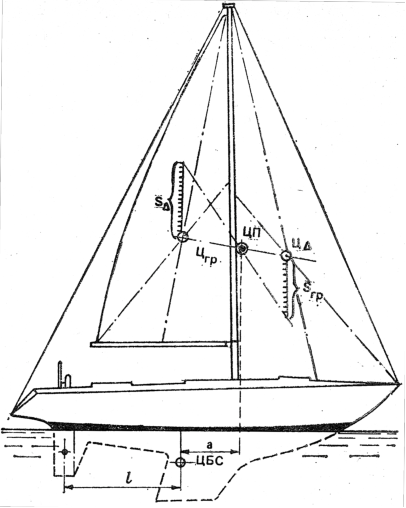
\includegraphics[scale=1.2]{0012P.pdf}
  \caption{Схема определения геометрического центра парусности яхты с вооружением типа <<шлюп>>}
  \label{fig:12}
\end{figure}

Поэтому при проектировании и перевооружении яхт оперируют с условными \textit{ЦП} и \textit{ЦБС}, считая их расположенными в центрах тяжести плоских фигур, которыми являются паруса, поставленные в диаметральной плоскости яхты, и подводные очертания \textit{ДП} с килем, плавниками и рулем (рис.~\ris{12}). 

Известно, что центр тяжести треугольного паруса располагается на пересечении двух медиан, а общий центр тяжести двух парусов находится на отрезке прямой, соединяющей \textit{ЦП} обоих парусов, и делит этот отрезок обратно пропорционально их площади. Обычно, в расчет принимается не фактическая площадь стакселя, а обмерная площадь переднего парусного треугольника. 

Положение \textit{ЦБС} можно определить, уравновешивая на острие иголки профиль подводной части \textit{ДП}, вырезанный из тонкого картона. Когда шаблон располагается строго горизонтально, игла находится в условной точке \textit{ЦБС}. Напомним, что в создании силы сопротивления дрейфу главная роль принадлежит плавниковому килю и рулю. Центры гидродинамических давлений на их профилях могут быть найдены достаточно точно, например, для профилей с относительной толщиной $t/b$ около 8\,\% эта точка находится на расстоянии около 26\,\% хорды от входящей кромки. Однако корпус яхты, хотя и участвует в создании поперечной силы в малой степени, вносит определенные изменения в характер обтекания киля и руля, причем он изменяется в зависимости от угла крена и дифферента, а также скорости яхты. В большинстве случаев на курсе бейдевинд истинный \textit{ЦБС} перемещается вперед. 

Конструкторы, как правило, располагают \textit{ЦП} на некотором расстоянии (опережении) впереди \textit{ЦБС}. Обычно опережение задается в процентах длины судна по ватерлинии и составляет для бермудского шлюпа 15\otdo 18\,\% \lkvl.

Если истинный \textit{ЦП} оказывается расположенным слишком далеко впереди \textit{ЦБС}, яхта на курсе бейдевинд уваливается под ветер и рулевому приходится постоянно держать руль отклоненным на ветер. Если же \textit{ЦП} оказывается позади \textit{ЦБС}, то яхта стремится привестись к ветру; требуется постоянная работа рулем, чтобы сдерживать судно. 

Особенно неприятна тенденция яхты к уваливанию. В случае аварии с рулем яхту не удается с помощью одних парусов привести на курс бейдевинд, кроме того, она обладает повышенным дрейфом. Дело в том, что киль яхты отклоняет стекающий с него поток воды ближе к \textit{ДП} судна. Поэтому если руль стоит прямо, он работает с заметно меньшим углом атаки, чем киль. Если отклонить руль в наветренную сторону, то образуемая на нем подъемная сила оказывается направленной в подветренную сторону \--- туда же, что и сила дрейфа на парусах. В данном случае киль и руль <<тянут>> в разные стороны и яхта неустойчива на курсе.

Иное дело легкая тенденция яхты приводиться. Переложенный на небольшой угол (3\otdo 4\gr) под ветер руль работает с таким же или несколько большим углом атаки, что и киль, и эффективно участвует в сопротивлении дрейфу. Поперечная сила, возникающая на руле, вызывает значительное смещение общего \textit{ЦБС} к корме, одновременно уменьшается угол дрейфа, яхта устойчиво лежит на курсе.

Однако если на курсе бейдевинд руль приходится постоянно перекладывать под ветер на большую величину, чем 3\otdo 4\gr, следует подумать о корректировке относительного положения \textit{ЦБС} и \textit{ЦП}. На уже построенной яхте это проще делать, перемещая вперед \textit{ЦП}, \--- устанавливая мачту в степсе в крайнее носовое положение или наклоняя её вперед. Причиной приведения яхты может быть также грот \--- слишком <<пузатый>> или с перебранной задней шкаториной. В этом случае полезен промежуточный штаг, с помощью которого можно придать мачте в средней части (по высоте) прогиб вперед и тем самым сделать парус более плоским, а также ослабить заднюю шкаторину. Можно также укоротить длину нижней шкаторины грота. 

Сложнее сместить в корму \textit{ЦБС}, для чего нужно установить кормовой плавничок перед рулем или увеличить площадь пера руля.

Мы уже говорили, что при увеличении крена увеличивается, и тенденция яхты приводиться. Это происходит не только вследствие увеличения плеча приводящей пары сил \--- \ve T и \ve R. При крене гидродинамическое давление в районе носовой волны повышается, что приводит к смещению \textit{ЦБС} вперед. Поэтому в свежий ветер для уменьшения тенденции яхты приводиться следует переместить вперед и \textit{ЦП}: взять риф на гроте или немного перетравить его для данного курса. Полезно также сменить стаксель на меньший по площади, благодаря чему уменьшается крен и дифферент яхты на нос.

Опытный конструктор при выборе величины опережения а обычно учитывает остойчивость яхты, чтобы компенсировать рост приводящего момента при крене: для яхты с меньшей остойчивостью задается большая величина опережения, для более остойчивых судов опережение принимается минимальным.

Хорошо уцентрованные яхты часто обладают повышенной рыскливостью на курсе бакштаг, когда потравленный на борт грот стремится развернуть яхту носом к ветру. Этому помогает и высокая волна, набегающая с кормы под углом к ДП. Чтобы одерживать яхту на курсе, приходится сильно работать рулем, отклоняя его на критический угол, когда возможен срыв потока с его подветренной поверхности (обычно это случается при углах атаки a 15\otdo 20\gr). Это явление сопровождается потерей подъемной силы на руле и, следовательно, управляемости яхты. Яхта внезапно может резко броситься к ветру и получить большой крен, при этом из-за уменьшения углубления пера руля на сторону разрежения может прорваться воздух с поверхности воды. 

Борьба с этим явлением, получившим название \textbf{брочинг}, заставляет увеличивать площадь пера руля и его удлинение, устанавливать перед рулем плавник, площадь которого составляет около четверти площади пера. Благодаря наличию плавника перед рулем организуется направленный поток воды, увеличиваются критические углы атаки руля, предотвращается прорыв воздуха к нему и уменьшается усилие на румпеле. При плавании в бакштаг экипаж должен стремиться к том чтобы тяга спинакера была направлена по возможности вперед, а не вбок чтобы избежать излишнего крена. Важно также препятствовать появлению дифферента на нос, при котором может уменьшиться углубление руля. Брочингу способствует также бортовая качка яхты, появляющаяся вследствие срывов потока воздуха со спинакера.

Устойчивость на курсе помимо рассмотренного влияния внешних сил и взаимного расположения их точек приложения определяется конфигурацией подводной части \textit{ДП}. Ранее для дальних плаваний по открытой воде отдавали предпочтение яхтам с длинной килевой линией, как обладающим большим сопротивлением повороту и соответственно \--- устойчивостью на курсе. Однако этому типу судов свойственны существенные недостатка например большая смоченная поверхность и плохая поворотливость. К тому же выяснилось, что устойчивость на курсе зависит не столько от величины боковой проекции \textit{ДП}, сколько от положения руля относительно \textit{ЦБС}, т.\=,е. от <<рычага>>, на котором действует руль. Отмечено, что если это расстояние оказывается менее 25\,\% \lkvl, то яхта становится рыскливой и плохо реагирует на отклонение руля. При $l = 40 \motdo 45\,\%$ \lkvl (см. рис.~\ris{12}) удержание судна на заданном курсе не составляет труда.

\begin{figure*}[htb]
  \centering
  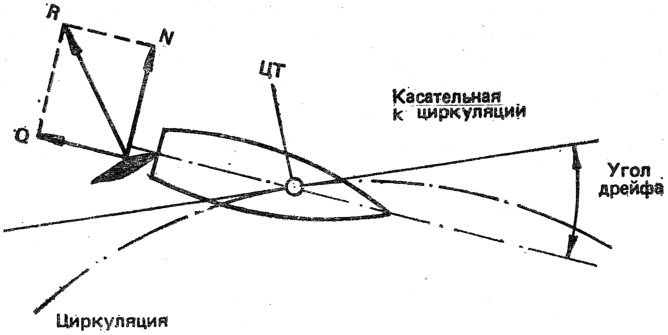
\includegraphics{0013P.pdf}
  \caption{Действие руля и схема движения яхты на циркуляции}
  \label{fig:13}
\end{figure*}

\textbf{Поворотливость} \--- способность судна изменять направление движения, описывать траекторию под действием руля и парусов. Действие руля основано на том же принципе гидродинамического крыла, что рассматривался и для яхтенного киля. При перекладке руля на некоторый угол возникает гидродинамическая сила \ve R, одна из составляющих которой \ve N толкает корму яхты в сторону, противоположную той, в которую положен руль (рис.~\ris{13}). Под её действием судно начинает двигаться по кривой траектории. Одновременно сила \ve R дает составляющую \ve Q \--- силу сопротивления, тормозящую ход яхты.

Если закрепить руль в одном положении, то судно пойдет примерно по окружности, называемой циркуляцией. Диаметр или радиус циркуляции является мерой поворотливости судна: чем больше радиус циркуляции, тем хуже поворотливость. По циркуляции движется только центр тяжести яхты, корму выносит наружу. Одновременно судно получает дрейф, вызванный центробежной силой и отчасти силой \ve N на пере руля.

Радиус циркуляции зависит от скорости и массы яхты, её момента инерции относительно вертикальной оси, проходящей через \textit{ЦТ}, от эффективности руля \--- величины силы \ve N и её плеча относительно \textit{ЦТ} при данном отклонении руля. Чем больше скорость и водоизмещение яхты, чем больше тяжелых масс (двигатель, якоря, детали оборудования) размещено в оконечностях судна, тем больше радиус циркуляции. Обычно радиус циркуляции, определенный на ходовых испытаниях яхты, выражают в длинах корпуса.

Поворотливость тем лучше, чем короче подводная часть судна и чем ближе к миделю сконцентрирована её основная площадь. Плохой поворотливостью обладают, например, суда с длинной килевой линией (типа военно\-/морских шлюпок) и, наоборот, хорошей \--- швертботы с узкими глубокими швертами. 

Эффективность руля зависит от площади и формы пера, профиля поперечного сечения, аэродинамического удлинения, типа установки (на ахтерштевне, отдельно от киля или на плавнике), а также расстояния баллера от \textit{ЦБС}. Наибольшее распространение получили рули, спроектированные в виде крыла с аэродинамическим профилем поперечного сечения. Максимальной толщина профиля принимается обычно в пределах 10\otdo 12\,\% хорды и располагается на 1/3 хорды от передней кромки. Площадь руля составляет обычно 9,5\otdo 11\,\% площади погруженной части \textit{ДП} яхты. 

Руль с большим удлинением (отношение квадрата глубины погружения руля к его площади) развивает большую поперечную силу на малых углах атаки, благодаря чему он эффективно участвует в обеспечении боковой силы сопротивления дрейфу. Однако, как было показано на рис.~\ris{11}, на определенных углах атаки профилей различного удлинения происходит отрыв потока от поверхности разрежения, после чего подъемная сила на профиле существенно падает. Например, при $\lambda = 6$ критический угол перекладки руля составляет 15\gr; при $\lambda = 2$ составляет 30\gr. В качестве компромисса применяют рули с удлинением $\lambda = 4 \motdo 5$ (соотношение сторон прямоугольного руля 2\otdo 2,5), а для повышения критического угла перекладки устанавливают перед рулем плавник\-/скег. Руль с большим удлинением быстрее реагирует на перекладку, так как циркуляция потока, обусловливающая подъемную силу, быстрее развивается вокруг профиля с малой хордой, чем вокруг всей подводной части корпуса с навесным на ахтерштевне рулем. 

Верхняя кромка руля должна плотно прилегать к корпусу в пределах рабочих отклонений $\pm 30\gr$, чтобы препятствовать перетеканию воды через нее; в противном случае эффективность работы руля ухудшается. Иногда на пере руля, если он навешен на транце, закрепляют аэродинамическую шайбу в виде широкой пластины близ ватерлинии.

Сказанное о форме килей применимо и к рулям: оптимальной считается трапециевидная форма с прямоугольной либо слегка скругленной нижней кромкой. Для уменьшения усилий на румпеле руль иногда делают балансирного типа \--- с осью вращения, расположенной на 1/4\otdo 1/5 хорды от <<носика>> профиля.

При управлении яхтой необходимо учитывать специфику работы руля в различных условиях, и, прежде всего срыв потока с его спинки. Нельзя делать резких перекладок руля на борт в начале поворота \--- произойдет срыв потока, поперечная сила \ve N на руле упадет, зато быстро увеличится сила сопротивления \ve R. Яхта будет входить в циркуляцию медленно и с большой потерей скорости. Начинать поворот необходимо, переложив руль на небольшой угол, но как только корма покатится наружу, и угол атаки руля начнет уменьшаться, его следует переложить на больший угол относительно \textit{ДП} яхты. 

Следует помнить, что поперечная, сила на руле быстро возрастает с увеличением скорости яхты. В слабый ветер бесполезно пытаться повернуть яхту быстро, перекладывая руль на большой угол (кстати, величина критического угла зависит от скорости: на меньшей скорости отрыв потока происходит при меньших углах атаки).

Сопротивление руля при изменении курса яхты в зависимости от его формы, конструкции и расположения составляет от 10 до 40\,\% общего сопротивления яхты. Поэтому к технике управления рулем (и к центровке яхты, от которой зависит устойчивость на курсе) надо относиться весьма серьезно, не допускать отклонения руля на больший угол, чем это необходимо.

\section{Ходкость}

\textbf{Ходкостью} называют способность яхты развивать определенную скорость при эффективном использовании энергии ветра.

Скорость, которую может развить яхта, зависит прежде всего от скорости ветра, поскольку все аэродинамические силы, действующие на парус в том числе и сила тяги, возрастав пропорционально квадрату скорости вымпельного ветра. Кроме того, она зависит и от энерговооруженности судна \--- отношения площади парусности к его размерениям. В качестве характеристики энерговооруженности чаще всего применяют отношение $S^{1/2} / V^{1/3}$
(где $S$ \--- площадь парусности\msq; $V$ \--- полное водоизмещение, м$^3$); или $S / \Omega$ 
(здесь $\Omega$ \--- смоченная поверхность корпуса, включая киль и руль). Сила тяги, а, следовательно, и скорость яхты, определяется еще и способностью парусного вооружения развивать достаточную тягу на различных курсах по отношению к направлению ветра.

Перечисленные факторы относятся к парусам \--- движителю яхты, преобразующему энергию ветра в движущую силу \ve T. Как было показано на рис.~\ris{4}, эта сила при равномерном движении яхты должна быть равна и противоположно направлена силе сопротивления движению \ve R. Последняя представляет собой проекцию результирующих всех гидродинамических сил, действующих на смоченную поверхность корпуса, на направление движения.

Различают два рода гидродинамических сил: силы давления, направленные перпендикулярно поверхности корпуса, и силы вязкости, действующие по касательной к этой поверхности. Результирующая сил вязкости дает силу \textbf{сопротивления трения}. 

Силы давления обусловлены образованием при движении яхты волн на поверхности воды, поэтому их результирующая дает силу \textbf{волнового сопротивления}. 

При большой кривизне поверхности корпуса в кормовой части пограничный слой может отрываться от обшивки, могут образовываться завихрения, поглощающие часть энергии движущей силы. Так возникает еще одна составляющая сопротивления движению яхты \--- \textbf{сопротивление формы}.

Еще два вида сопротивления появляются в связи с тем, что яхта движется не прямо вдоль \textit{ДП}, а с некоторым углом дрейфа и с креном. Это \textbf{индуктивное} и \textbf{креновое} сопротивления. Существенную долю в индуктивном сопротивлении занимает сопротивление выступающих частей \--- киля и руля.

Наконец, движению яхты вперед оказывает сопротивление и воздух, омывающий корпус, экипаж, развитую систему тросов такелажа и паруса. Эта часть сопротивления носит название \textbf{воздушного}. 

\textbf{Сопротивление трения.} При движении яхты частицы воды, непосредственно примыкающие к обшивке корпуса, как бы прилипают к ней и увлекаются вместе с судном. Скорость этих частиц относительно корпуса равна нулю (рис.~\ris{14}). Следующий слой частиц, скользя по первому, уже немного отстает от соответствующих точек корпуса, а на определенном расстоянии от обшивки вода вообще остается неподвижной или имеет скорость относительно корпуса, равную скорости яхты $v$. Этот слой воды, в котором действуют силы вязкости, а скорость движения частиц воды относительно корпуса возрастает от 0 до скорости судна, называется пограничным слоем. Толщина его относительно невелика и составляет от 1 до 2\,\% длины корпуса по ватерлинии, однако характер или режим движения частиц воды в нем оказывает существенное влияние на величину сопротивления трения.

\begin{figure*}[htb]
  \centering
  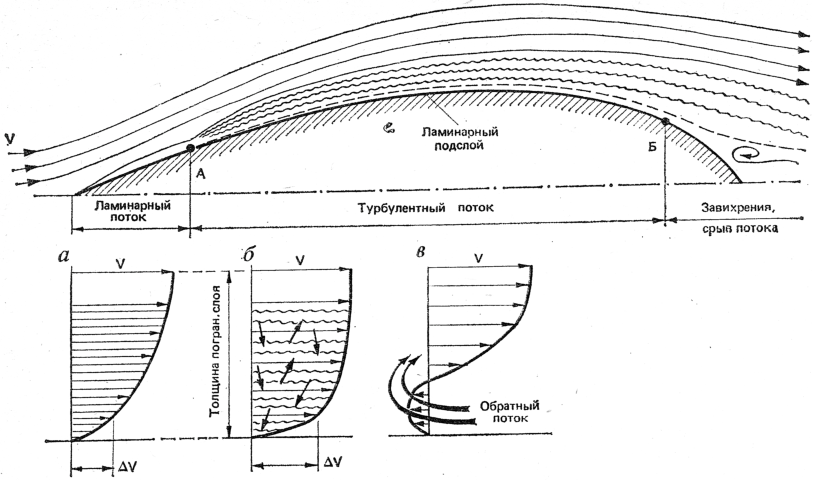
\includegraphics[scale=1.3]{0014P.pdf}
  \caption{Потоки жидкости около корпуса яхты}
  \label{fig:14}
  \small
  \centering{}
  \textit{А} \--- точка перехода ламинарного пограничного слоя в турбулентный; \textit{Б} \--- точка отрыва потока от корпуса; \textit{а} \--- изменение скоростей потока в ламинарном пограничном слое; \textit{б} \--- изменение скоростей потока в турбулентном слое; \textit{в} \--- изменение скоростей в пограничном слое в корму от точки \textit{Б}
\end{figure*}

Установлено, что режим движения частиц изменяется в зависимости от скорости судна и длины его смоченной поверхности. В гидродинамике эта зависимость выражается числом Рейнольдса:

\begin{equation}
  \Renum = \frac{v \cdot L}{\nu} \quad , 
\end{equation}

где: $\nu$ \--- коэффициент кинематической вязкости воды (для пресной воды $\nu = 1,15 \cdot 10^{-6} \text{м}^2/\text{с})$; $L$ \--- длина смоченной поверхности, м; $v$ \--- скорость яхты, м/с. 

При относительно небольшом числе $\Renum = 10^6$ частицы воды в пограничном слое движутся слоями, образуя ламинарный поток. Его энергии оказывается недостаточно, чтобы преодолеть силы вязкости, препятствующие поперечным перемещениям частиц. Наибольший перепад скорости между слоями частиц оказывается непосредственно у поверхности корпуса; соответственно и силы трения имеют здесь наибольшую величину. 

Число Рейнольдса в пограничном слое увеличивается по мере удаления частиц воды от форштевня (с возрастанием смоченной длины). При скорости 2 м/с, например, уже на расстоянии около 2 м от него Re достигнет критической величины, при которой режим потока в пограничном слое становится вихревым, т.\=,е. турбулентным и направленным поперек пограничного слоя. Вследствие возникшего обмена кинетической энергией между слоями скорость частиц близ поверхности корпуса растет в большей степени, чем при ламинарном потоке. Перепад скоростей $\Delta v$ здесь возрастает, соответственно растет и сопротивление трения. Вследствие поперечных движений частиц воды толщина пограничного слоя увеличивается, а сопротивление трения резко увеличивается. 

Ламинарный режим обтекания охватывает только небольшую часть корпуса яхты в носовой его части только на малых скоростях. Критическая величина Re, при которой возникает турбулентное обтекание корпуса, лежит в пределах $5 \cdot 10^5\motdo 6 \cdot 10^6$ и в значительной степени зависит от формы и гладкости поверхности его. При повышении скорости точка перехода, ламинарного пограничного слоя в турбулентный перемещается в сторону носа. При достаточно высокой скорости может наступить момент, когда вся смоченная поверхность корпуса будет охвачена турбулентным потоком. Правда, непосредственно около обшивки, где скорость обтекания близка к нулю, все же сохраняется тончайшая пленка с ламинарным режимом \--- ламинарный подслой. 

Сопротивление трения рассчитывают по формуле:

\begin{equation}
  \cidx{R}{ТР} = \cidx{\zeta}{ТР} \cdot \frac{\rho \cdot v^2}{2} \cdot \Omega, \quad \text{кгс}, 
\end{equation}

где: \cidx{R}{ТР} \--- сопротивление трения, кг; \cidx{\zeta}{ТР} \--- коэффициент сопротивления трения; $\rho$ \--- массовая плотность воды; для пресной воды: $\rho = 102\, \text{кг} \cdot \text{с}^2/\text{м}^4$; $v$ \--- скорость яхты, м/с; $\Omega$ \--- смоченная поверхность,\msq. 

Коэффициент сопротивления трения \--- величина переменная, зависящая от характера потока в пограничном слое, длины корпуса \lkvl, скорости $v$ и шероховатости поверхности корпуса.

На рис.~\ris{15} показaнa зависимость коэффициента сопротивления трения \cidx{\zeta}{ТР} от числа Re и шероховатости поверхности корпуса.

\begin{figure*}[htb]
  \centering
  \includegraphics[scale=1.3]{0015P.pdf}
  \caption{Коэффициент сопротивления трения технически гладкой и шероховатых поверхностей в зависимости от числа Рейнольдса \Renum}
  \label{fig:15}
\end{figure*}

Рост сопротивления шероховатой поверхности по сравнению с гладкой нетрудно объяснить наличием в турбулентном пограничном слое ламинарного подслоя. Если бугорки на поверхности полностью погружены в ламинарный подслой, то они не вносят существенных изменений в характер ламинарного течения подслоя. Если же неровности превышают толщину подслоя и выступают над ним, то происходит турбулизация движения частиц воды по всей толщине пограничного слоя, и коэффициент трения соответственно возрастает.

Рис.~\ris{15} позволяет оценить важность отделки днища яхты для снижения её сопротивления трения. Например, если яхта длиной 7,5\,м по ватерлинии идет со скоростью $v = 6$ узл. (3,1\,м/с), то соответствующее число $\Renum = (3,1 \cdot 7,5) / (1,15 \cdot 10^{-6} ) = 2 \cdot 10^7$. 

Допустим, что днище яхты имеет шероховатость (среднюю высоту неровностей) $k = 0,2$\,мм, что соответствует относительной шероховатости $L/k = 7500 / 0,2 = 3,75 \cdot 10^4$.

Для данной шероховатости и числа Rе коэффициент трения равен $\cidx{\zeta}{ТР} = 0,0038$ (точка Г).

Оценим, можно ли получить в данном случае поверхность днища, близкую к технически гладкой. При $\Renum = 2 \cdot 10^7$ такой поверхности соответствует относительная шероховатость $L/k = 3 \cdot 10^5$ или абсолютная шероховатость $k = 7500/3 \cdot 10^5 = 0,025$\,мм. Опыт показывает, что этого можно добиться, тщательно отшлифовав днище мелкой шкуркой, а затем отлакировав его. Оправдаются ли затраченные усилия? График показывает, что коэффициент сопротивления трения снизится до $\cidx{\zeta}{ТР} = 0,0028$ (точка Д), или на 30\,\%, чем, конечно, не может пренебрегать экипаж, рассчитывающий на успех в гонках.

Линия Б позволяет оценить допустимую шероховатость днища для яхт различных размеров и различной скорости. Можно заметить, что с увеличением длины по ватерлинии и скорости требования к качеству поверхности возрастают. 

Для ориентировки приведем значения шероховатости (в мм) для различных поверхностей:
\begin{itemize}
\item деревянная, тщательно лакированная и шлифованная \--- 0,003\otdo 0,005; 
\item деревянная, окрашенная и шлифованная \--- 0,02\otdo 0,03; 
\item окрашенная патентованным покрытием \--- 0,04\otdo 0,06; 
\item деревянная, окрашенная суриком \--- 0,15; 
\item обычная доска \--- 0,5; 
\item обросшее ракушками днище \--- до 4,0.
\end{itemize}

Мы уже говорили, что на части длины яхты, начиная от форштевня, может сохраняться ламинарный пограничный слой, если только излишняя шероховатость не будет способствовать турбулизации потока. Поэтому особенно важно тщательно обрабатывать носовую часть корпуса, все входящие кромки киля, плавников и рулей. При малых поперечных размеpax \--- хордах следует шлифовать всю поверхность киля и руля. В кормовой части корпуса, где толщина пограничного слоя увеличивается, требования к отделке поверхности могут быть несколько снижены. 

Особенно сильно отражается на сопротивлении трения обрастание днища водорослями и ракушками. Если периодически не очищать днище яхт, постоянно находящихся в воде, то через два--три месяца сопротивление трения может увеличиться на 50\otdo 80\,\%, что равносильно потере скорости в средний ветер на 15\otdo 25\,\%. 

\textbf{Сопротивление формы.} Даже у хорошо обтекаемого корпуса на ходу можно обнаружить кильватерный след \--- струю, в которой вода совершает вихревые движения. Это следствие отрыва от корпуса пограничного слоя в определенной точке (Б на рис.~\ris{14}). Положение точки зависит от характера изменения кривизны поверхности по длине корпуса. Чем плавнее обводы кормовой оконечности, тем дальше к корме происходит отрыв пограничного слоя и меньше вихреобразование. 

При нормальных соотношениях длины корпуса к ширине сопротивление формы невелико. Увеличение его может быть обусловлено наличием острых скул, сломов обводов корпуса, правильно спрофилированных килей, рулей и других выступающих частей. Сопротивление формы увеличивается с уменьшением протяженности зоны ламинарного пограничного слоя, этому следует снять наплывы краски, уменьшить шероховатость, заделать выемки в обшивке, поставить обтекатели на выступающие патрубки и т.\=,п.

\textbf{Волновое сопротивление.} Возникновение волн у корпуса судна при движении вызвано действием сил тяжести жидкости на границе раздела воды и воздуха. В носовой оконечности, в месте встречи корпуса с водой, давление резко повышается, и вода поднимается на некоторую высоту. Ближе к миделю, где вследствие расширения корпуса судна скорость обтекающего потока увеличивается, давление в нем, согласно закону Бернулли, падает, и уровень воды понижается. В кормовой части, где давление вновь повышается, образуется вторая вершина волны. Частицы воды начинают совершать колебания вблизи корпуса, которые вызывают вторичные колебания поверхности воды.

\begin{figure*}[htb]
  \centering
  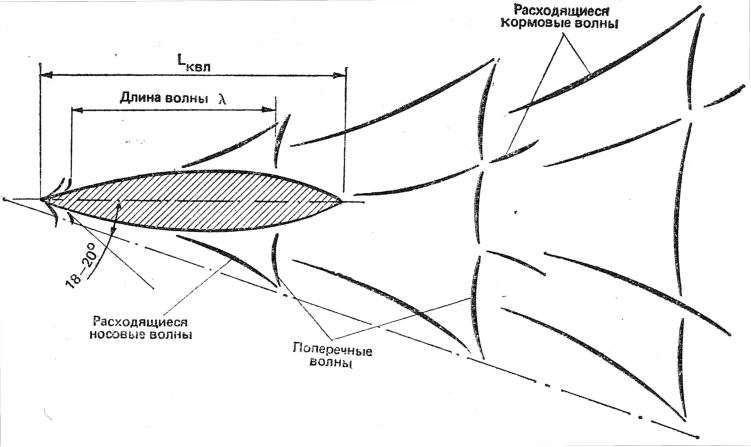
\includegraphics[scale=1.3]{0016P.pdf}
  \caption{Схема волновой системы, образующейся у корпуса судна}
  \label{fig:16}
\end{figure*}

Возникает сложная система носовых и кормовых волн, которая по своему характеру одинакова для судов любых размеров (рис.~\ris{16}). На малой скорости хорошо заметны расходящиеся волны, зарождающиеся в носу и корме судна. Их гребни расположены под углом 36\otdo 40\gr к диаметральной плоскости. На более высоких скоростях выделяются поперечные волны, гребни которые не выходят за пределы сектора, ограниченного углом 18\otdo 20\gr к \textit{ДП} судна. Носовая и кормовая системы поперечных волн взаимодействуют друг с другом, следствием чего может быть как увеличение высоты суммарной волны за кормой судна, так и её уменьшение. По мере удаления от судна энергия волн поглощается средой, и они постепенно затухают.

Величина волнового сопротивления изменяется в зависимости от скорости яхты. Из теории колебаний известно, что скорость распространения волн связана с их длиной $\lambda$ соотношением

\begin{equation}
  \lambda = \frac{2 \pi \cdot v^2}{\mathrm g}\,, \quad \text{м},
\end{equation}

где: $v$ \--- скорость яхты, м/с; $\mathrm g$ = 9,81 м/с$^2$ \--- ускорение силы тяжести. 

Поскольку волновая система движется вместе с яхтой, то и скорость распространения волны равна скорости яхты. Таким образом, можно подсчитать длину поперечной волны для каждой скорости яхты:

\begin{table*}[htb]
  \small
  \centering
  \begin{tabular}{l|c|c|c|c|c|c}
    \toprule
    Скорость, уз & 2 & 4 & 6 & 8 & 10 & 12 \\
    \midrule
    Длина волны, м & 0,68 & 2,72 & 6,12 & 10,9 & 17 & 24,5 \\
    \bottomrule
  \end{tabular}
  \caption{Зависимость длины поперечной волны от скорости яхты}
  \label{tab:1-2}
\end{table*}

Если речь идет, например, о яхте длиной по ватерлинии 8 м, то при скорости 4 уз на длине корпуса разместится около трех поперечных волн, при скорости 6 уз \--- полторы. Зависимость между длиной поперечной волны $\lambda$, создаваемой корпусом длиной \lkvl движущимся со скоростью $v$, во многом определяет величину волнового сопротивления. 

Для величины сопротивления важно, какая часть носовой поперечной волны подойдет к месту, где расположен гребень кормовой волны. Если на длине яхты по \textit{КВЛ} уложится целое число полуволн, то в корме может оказаться либо вершина, либо подошва носовой поперечной волны. Произойдет соответственно неблагоприятная (рис.~\ris{17}, \textit{б}) или благоприятная (рис.~\ris{17}, \textit{а}) интерференция волн. В первом случае высота суммарной волны возрастает и, поскольку энергия волн и величина волнового сопротивления пропорциональны квадрату их амплитуд, сопротивление яхты существенно возрастает. При благоприятном сложении подошвы носов волны с вершиной кормовой суммарная высота волны снизится, сопротивление увеличится медленнее.

\begin{figure*}[htb]
  \centering
  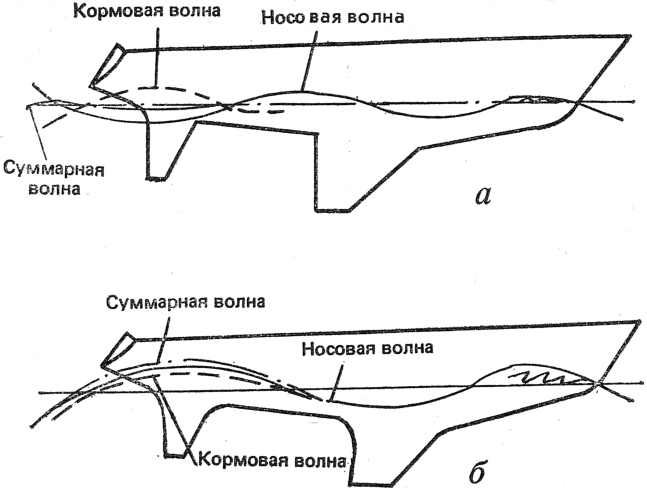
\includegraphics[scale=1.3]{0017P.pdf}
  \caption{Интерференция носовой и кормовой поперечных волн}
  \label{fig:17}
  \centering
  \small
  \textit{а} \--- благоприятная;
  \textit{б} \--- неблагоприятная
\end{figure*}

Многочисленными исследованиями, проведенными на моделях в опытном бассейне и на натурных судах, ycтановлено, что характер волнообразования всех судов, независимо от их размерений и абсолютной скорости, оказывается одинаков, если равны их относительные скорости или числа Фруда:

\begin{equation}
  \mathrm{Fr} = \frac{v}{(\mathrm g \cdot \lkvl)^{1/2}}
\end{equation}

Заметим, что в формулу относительной скорости входят длина судна по ватерлинии и те же символы, что и в формулу для определения длины волны в зависимости от её скорости. Этим подчеркивается взаимосвязь гравитационного характера волнообразования и его зависимость от скорости и длины судна.

На малых скоростях при $\mathrm{Fr} = 0,1\motdo 0,2$ волновое сопротивление яхты невелико. При $\mathrm{Fr} = 0,2$ на длине корпуса укладывается примерно четыре невысокие носовые поперечные волны. По мере повышения скорости волновое сопротивление начинает быстро расти. При числах Fr, равных 0,25, 0,30 и 0,50, имеет место неблагоприятная интерференция поперечных волн, а относительная скорость $\mathrm{Fr} = 0,5\motdo 0,6$ является порогом, превысить который обычная яхта водоизмещающего типа не может ни при каких обстоятельствах. На этой скорости яхта оказывается зажатой между двумя гребнями одной поперечной волны: сопротивление её возрастает пропорционально шестой степени скорости. Как правило, тяги парусов, даже при форсировании ими в свежий ветер, оказывается недостаточно, чтобы получить хотя бы небольшой прирост скорости. Поэтому скорость, соответствующую числу Фруда около 0,5, считают предельной для водоизмещающих яхт. Её можно вычислить, учитывая, что g \--- величина постоянная, по формуле\footnote{При переводе скорости из метрических мер в узлы и наоборот следует учитывать, что 1 узел = 1,852 км/ч = 0,514 м/с.}:

\begin{equation}
  v = 3 \cdot {\lkvl}^{1/2}, \quad \text{уз} 
\end{equation}

Таким образом, реальная скорость, которой могут достичь яхты отдельных типов, составляет около: 
\begin{itemize}
\item класс <<Солинг>> \--- 7,5 уз; 
\item тип <<Алькор>> \--- 9 уз; 
\item тип <<Конрад-54>> \--- 11,2 уз; 
\item класс R12 \--- 12 уз.
\end{itemize}

В ряде случаев в океанских гонках крейсерских яхт, однако, достигались более высокие скорости, которые могли развить в течение ограниченного времени суда облегченного типа. Это происходило, как правило, на попутных курсах и при крупной волне, при штормовых ветрах и форсировании парусами. В момент, когда под яхту подкатывался гребень очередной волны, смоченная поверхность корпуса резко уменьшалась и судно, выходило на режим серфинга \--- скольжения вместе с гребнем ветровой волны. При этом на яхте длиной по КВЛ 19,8 м, например, была отмечена максимальная скорость 22 уз ($v = 4,95 \cdot \lkvl$).

\begin{figure*}[htb]
  \centering
  \includegraphics[scale=1.3]{0018P.pdf}
  \caption{Зависимость сопротивления воды движению яхты от её скорости}
  \label{fig:18}
\end{figure*}

Как видно на рис.\ris{18}, доля волнового сопротивления в общем балансе сопротивления воды движению яхты возрастает с увеличением скорости яхты. На предельных скоростях оно достигает 60\otdo 65\,\%, а при движении в слабый ветер на создание волн затрачивается около 30\,\% движущей силы парусов. Поэтому снижение волнового сопротивления особенно важно для яхт, от которых ожидают хороших результатов в свежий ветер. При разработке проекта таких яхт стараются облегчить корпус и оборудование, чтобы значение относительной длины было в пределах $\lkvl / D^{1/3} = 4,2\motdo 5,2$ (чем больше эта длина, тем меньше волновое сопротивление). Коэффициент продольной полноты $\varphi$ принимают равным 0,60, чтобы более равномерно распределить водоизмещение яхты по длине и уменьшить глубину волновой впадины вблизи миделя.

Большое влияние на волновое сопротивление оказывает и отношение $\lkvl / \bkvl$. Благодаря большому удлинению корпусов катамаранов ($\lkvl / \bkvl = 10\motdo 20$) и отсутствию на них тяжелых фальшкилей удается существенно снизить их волновое сопротивление и достичь гораздо более высоких скоростей, чем $3 \cdot {\lkvl}^{1/2}$. Например, катамаран типа <<Центаурус>> ($\lkvl = 10$\,м) при благоприятных условиях развивает скорость 18 уз ($\approx 5,8 \cdot {\lkvl}^{1/2}$). 

\textbf{Дополнительное сопротивление на взволнованном море.} Нередко яхтсмены обнаруживают, что после многих часов, затраченных на лавировку против волны, яхта выбирается на ветер считанные мили. И это после изматывающей килевой качки! 

В данном случае приходится считаться с дополнительным сопротивлением движению яхты, которое появляется вследствие килевой качки судна. Особенно заметно падение скорости яхты, если период ее собственных продольных колебаний совпадает с периодом волны, т.\=,е. при резонансе. В существовании же собственных колебаний можно убедиться, если, например, спрыгнуть с носа яхты на причал. Каждая яхта при этом ведет себя, по-разному: у одной качка порывистая скоро затухает, у другой \--- плавная продолжается долго. 

Установлено, что период собственных продольных колебаний яхты зависит от продольного момента инерции т.\=,е. от расположения масс по длине судна, от обводов корпуса, особенно в оконечностях, взаимного расположения центра тяжести площади ватерлинии и центра тяжести яхты. Если, например, \textit{ЦТ} площади ватерлинии совпадает с \textit{ЦТ} яхты. Большие массы (якоря с цепями, двигатель цистерны топлива и пресной воды и т.\=,п.) расположены далеко от миделя и обводы, носа и кормы почти симметричны, яхта имеет достаточно большой период и амплитуду собственных колебаний, который может оказаться близким к периоду наиболее неблагоприятной волны длиной от 0,8 до 1,5 длины яхты по \textit{КВЛ}. При сильной килевой качке яхта приводит в движение большие массы воды, непосредственно соприкасающиеся с корпусом, таким образом, поглощается часть энергии ветра, которая могла бы затрачиваться на продвижение судна вперед, а сопротивление воды повышается 2\otdo 25 раза (по сравнению с тихой волны). 

При проектировании яхт обычно предусматривается возможность уменьшения размахов оконечностей яхты и смягчения качки. Наиболее тяжелые массы (фальшкиль, мачту, двигатель, цистерны и т.\=,п.) стараются расположить вблизи центра тяжести судна. Обводы корпуса выше ватерлинии обычно выполняются несимметричными относительно миделя. По мере движения кормы вниз ширина ватерлинии у транца и погружающийся объем корпуса прогрессивно увеличиваются, препятствуя глубокому погружению кормы в воду и поглощая энергию качки. Хороший развал надводного борта в носу также способствует снижению ускорений носовой части яхты при движении ее вниз.
 
Большое значение для уменьшения продольной качки имеет уменьшение массы рангоута и такелажа, поскольку момент инерции массы яхты складывается из произведения отдельных масс на квадраты отстояния их от \textit{ЦТ} судна. Таким образом, влияние на продольную качку килограмма массы на топе мачты, отстоящей от \textit{ЦТ} на 12\,м, аналогично грузу 70\,кг, расположенным на уровне палубы. 

Рис.~\ris{18} дает представление о доле добавочного сопротивления при ходе на волнении для крейсерско-гоночной яхты. При увеличении скорости эта составляющая общего сопротивления может возрасти до 15\otdo 25\,\%, что равносильно потере скорости на 3\otdo 4\,\%. Потеря существенно возрастает при резонансе, поэтому экипаж должен предпринять специальные меры для уменьшения амплитуды и изменения частоты колебаний. С этой целью можно изменить курс яхты по отношению к волне, если позволяют обстоятельства, или попытаться изменить период собственных колебаний судна, переместив людей на корму. Тогда яхта получит дифферент на корму, которая своим объемом и большой шириной ватерлинии будет гасить качку. 

\textbf{Дополнительное сопротивление от крена и дрейфа.} Испытания моделей яхт в опытных бассейнах показали, что с увеличением крена сопротивление корпуса превышает сопротивление тех же моделей, испытанных на ходу без крена. В качестве примера на рис.~\ris{18} дана кривая изменения дополнительного сопротивления яхты в зависимости от угла крена и скорости. При крене до 15\gr прирост сопротивления невелик \--- не более 5\,\%. Однако на скорости около 6 уз и при крене 35\gr сопротивление уже на 38\,\% больше, чем при плавании без крена. Для рассматриваемой яхты это приводит к потере 0,4 уз скорости. 

Эксперименты позволили выяснить, что дополнительное сопротивление в данном случае может быть разделено на две составляющие \--- индуктивное сопротивление и сопротивление от крена. Обе составляющие вызваны действием кренящей силы \vidx{F}{Д} (см. рис.~\ris{4}). Основным источником индуктивного сопротивления является подъемная сила на киле и руле, перетекание воды через нижнюю кромку плавников киля и руля со стороны повышенного давления на сторону разрежения, как мы уже говорили (см. рис.~\ris{20}). Срывающиеся с нижней кромки вихри требуют дополнительных затрат энергии движущей силы. Чем больше величина подъемной силы, образующейся на плавниках, тем больше разность давлений на их сторонах и соответственно больше индуктивное сопротивление. Наоборот, с увеличением аэродинамического удлинения плавника, т.\=,е. с уменьшением средней хорды относительно площади плавника, индуктивное сопротивление уменьшается. 

Определенную долю здесь вносит и корпус яхты, который обтекается не по оптимальным ватерлиниям, а под углом дрейфа. 

Дополнительное сопротивление от крена обусловлено как появлением несимметричности в обводах корпуса, так и изменением поля гидродинамических давлений у наветренного и подветренного бортов судна. У яхт с длинными свесами крен около 5\gr вызывает иногда даже некоторое снижение полного сопротивления при увеличении смоченной длины корпуса. Широкий <<швертботный>> современный корпус при крене 8\otdo 10\gr уменьшает смоченную поверхность и сопротивление, которое может снизиться на 2\otdo 4\,\%. Но с увеличением крена сопротивление начинает возрастать, составляя примерно 1/3 величины дополнительного сопротивления; остальное приходится на долю индуктивного сопротивления. И все же сопротивление от крена достаточно велико \--- оно достигает около 15\,\% сопротивления яхты, идущей без крена. Следовательно, при участии в гонке экипаж должен принять меры к уменьшению крена.

На рис.~\ris{18} хорошо видно, что крен 30\gr является для данной яхты критическим. Дальнейшее усиление ветра, при котором судно получает дополнительный крен, приводит уже не к повышению скорости, а, наоборот, к снижению. Значит, при достижении этого крена целесообразно уменьшить площадь парусности, а на небольшой яхте попытаться откренить судно массой экипажа.

При крене не только дополнительно растет сопротивление, но и ухудшается эффективность работы парусного вооружения, увеличивается склонность яхты приводиться к ветру. Для удержания судна на курсе необходимо отклонять руль на большой угол, что дополнительно увеличивает лобовое индуктивное сопротивление руля. 

Воздушное сопротивление корпуса яхты, рубок и экипажа, расположенного на палубе, сравнительно невелико. Оно достигает заметной величины только в сильный ветер и на курсе бейдевинд. Гораздо большее, значение имеет сопротивление рангоута, парусов и такелажа, рассмотрению которых уделено внимание в гл.~\ref{chap:2}.

\chapter{Прикладная аэродинамика паруса}\label{chap:2}

\section{Работа паруса}

Современная теория паруса основывается на положениях аэродинамики крыла, элементы которой были рассмотрены в главе <<Элементы теории парусной яхты>> (см. <<Сопротивление дрейфу>>). Механика возникновения аэродинамической силы на парусе, изготовленном из ткани, в принципе аналогична и для жесткого профилированного крыла. В любом поперечном сечении паруса должна развиться циркуляция потока воздуха, как вокруг профиля крыла (см. рис.~\ris{8}), чтобы появилась подъемная сила.

Естественно, что аэродинамика паруса из ткани имеет ряд существенных отличий от жесткого крыла, каким, например, является яхтенный киль. Вследствие эластичности ткани парус изменяет свой профиль под влиянием потока воздуха. Он обладает способностью скручиваться \--- изменять угол атаки по отношению к ветру по высоте. В отличие от получивших распространение аэродинамических профилей со сравнительно толстой входящей кромкой парус имеет острую переднюю кромку и выпукло\-/вогнутую форму, образованную тонким материалом. Наконец, передней кромкой парус может крепиться к мачте, имеющей довольно большое поперечное сечение, что вносит существенное изменение в картину обтекания паруса потоком и в распределении давления по ширине паруса.

\begin{figure}[htb]
  \centering
  \includegraphics[scale=1.2]{0019P.pdf}
  \caption{Схема сил, действующих на паруса яхты; основные угловые параметры движения и установки парусов}
  \label{fig:19}
  \centering{}
  \small
  $\beta$ \--- путь яхты по отношению к вымпельному ветру; $\lambda$ \--- угол дрейфа; $\alpha$ \--- угол атаки паруса; $\delta$ \--- угол установки паруса относительно \textit{ДП} яхты; \vidx{V}{И} \--- скорость истинного ветра; \ve V \--- скорость яхты; \vidx{V}{В} \--- скорость вымпельного ветра; \vidx{V}{НВ} \--- скорость прямо против ветра
\end{figure}

Наиболее важные элементы, влияющие на аэродинамику паруса, будут рассмотрены дальше, но для начала установим влияние составляющих аэродинамической силы на движение яхты при различных курсах относительно ветра.

Если яхта идет курсом бейдевинд, то под действием набегающего потока воздуха на парусах, установленных под углом атаки $\alpha$ к направлению вымпельного ветра, возникает результирующая аэродинамическая сила \ve A (рис.~\ris{19}). По аналогии с жестким крылом эту силу можно разложить на две составляющие: подъемную силу \ve Y, перпендикулярную направлению вымпельного ветра, и лобовое сопротивление \ve X, действующее по направлению ветра. В дальнейшем эти силы мы будем использовать для рассмотрения характеристик паруса и всего парусного вооружения в целом. 

Для того чтобы оценить влияние аэродинамической силы \ve A на движение яхты, представим ее в виде двух других составляющих: силы тяги \ve T, направленной по оси движения судна, и перпендикулярной ей силы дрейфа \ve D. Направление движения яхты (путь) отличается от ее курса на величину угла дрейфа $\lambda$, однако в дальнейшем анализе этим углом можно пренебречь. 

Предположим, что на выбранном курсе бейдевинд удалось увеличить подъемную силу на парусе до величины \vidx{Y}{1}, а лобовое сопротивление не изменилось. Силы \vidx{Y}{1} и \ve X, будучи сложенными по правилу сложения векторов, образуют новую аэродинамическую силу \vidx{A}{1}. Изменятся и ее составляющие относительно оси движения яхты \ve T и \ve D. Без вычислений можно сказать, что в данном случае с увеличением подъемной силы увеличатся и сила тяги, и сила дрейфа (рис.~\ris{20}). Аналогичное построение позволяет убедиться, что при увеличении лобового сопротивления на курсе бейдевинд сила тяги уменьшается, а сила дрейфа увеличивается. Таким образом, при плавании в лавировку экипаж яхты должен стремиться по возможности добиться образования на парусах максимальной подъемной силы при минимальной величине лобового сопротивления. Иными словами, для острых курсов необходима работа паруса с максимальным аэродинамическим качеством, которое численно выражается в отношении подъемной силы к лобовому сопротивлению. 

\begin{equation}
\ve K = \ve Y / \ve X
\end{equation}

Отметим, что на курсе бейдевинд вымпельный ветер, являющийся результатом сложения векторов истинного ветра и движения яхты, имеет наивысшую скорость \vidx{V}{В} (см. рис.~\ris{19}, \textit{б}), что сказывается на величине обеих составляющих аэродинамической силы \--- \ve Y и \ve X.

На курсе галфвинд подъемная сила является силой тяги, а лобовое сопротивление \--- силой дрейфа. Если лобовое сопротивление увеличить, то увеличится только сила дрейфа. Однако на ходовые качества яхты это влияет в заметно меньшей степени, чем на курсе бейдевинд, поскольку скорость вымпельного ветра на курсе галфвинд снизилась и, следовательно, величина силы дрейфа меньше.

\begin{figure*}[htb]
  \centering
  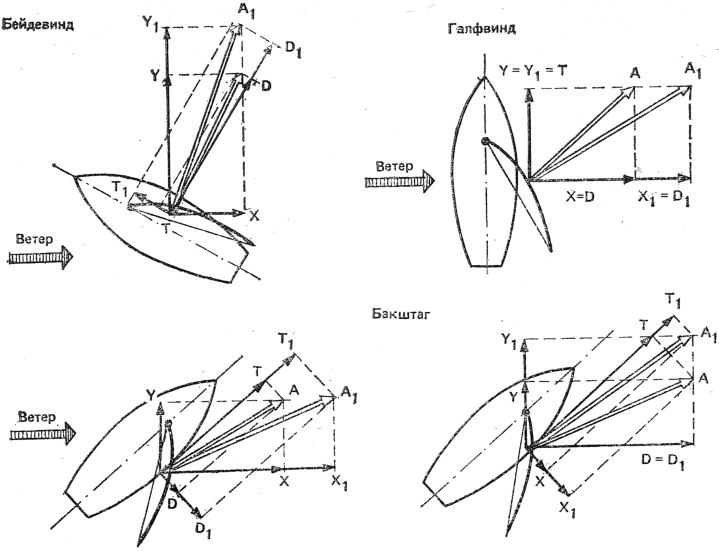
\includegraphics[scale=1.3]{0020P}
  \caption{Роль составляющих аэродинамической силы на различных курсах относительно вымпельного ветра}
  \label{fig:20}
\end{figure*}

На курсе бакштаг парус работает на больших углах атаки, при которых подъемная сила оказывается значительно меньше лобового сопротивления. Если увеличить лобовое сопротивление, то тяга и сила дрейфа увеличатся. При возрастании подъемной силы тяга также увеличивается, а сила дрейфа уменьшается. Следовательно, на курсе бакштаг рост и подъемной силы и (или) лобового сопротивления увеличивает тягу. Сила дрейфа тем больше, чем больше лобовое сопротивление. На курсе фордевинд угол атаки паруса близок к 90\gr, поэтому подъемная сила на парусе равна нулю, а лобовое сопротивление направлено по оси движения яхты и становится силой тяги. Сила дрейфа равна нулю. Следовательно, на курсе фордевинд для увеличения силы тяги нужно увеличивать лобовое сопротивление парусного вооружения, что на гоночных яхтах достигается постановкой дополнительных парусов \--- \textbf{спинакера} и \textbf{блупера}, имеющих большую площадь и плохо обтекаемую форму. 

Отметим, что на курсе фордевинд на паруса действует вымпельный ветер минимальной скорости, в результате чего на паруса действуют сравнительно умеренные силы.

\section{Особенности работы паруса как крыла}

Только при небольшом значении угла атаки, когда на остром и тонком профиле еще не образуется подъемная сила, парус обтекается потоком воздуха, одинаково плавным с нижней и с верхней стороны. При небольшом увеличении угла атаки критическая точка перемещается на нижнюю сторону профиля и потоку приходится огибать острую кромку с большой скоростью. В результате у входящей кромки образуется значительное разрежение и под влиянием этого разрежения пограничный слой отрывается от поверхности профиля, образуя на его спинке вихревой пузырь. При достаточно большой скорости ветра поток быстро поглощает энергию вихрей и слой вновь  присоединяется к поверхности профиля на некотором расстоянии от входящей кромки (рис.~\ris{21}).

\begin{figure*}[htb]
  \centering
  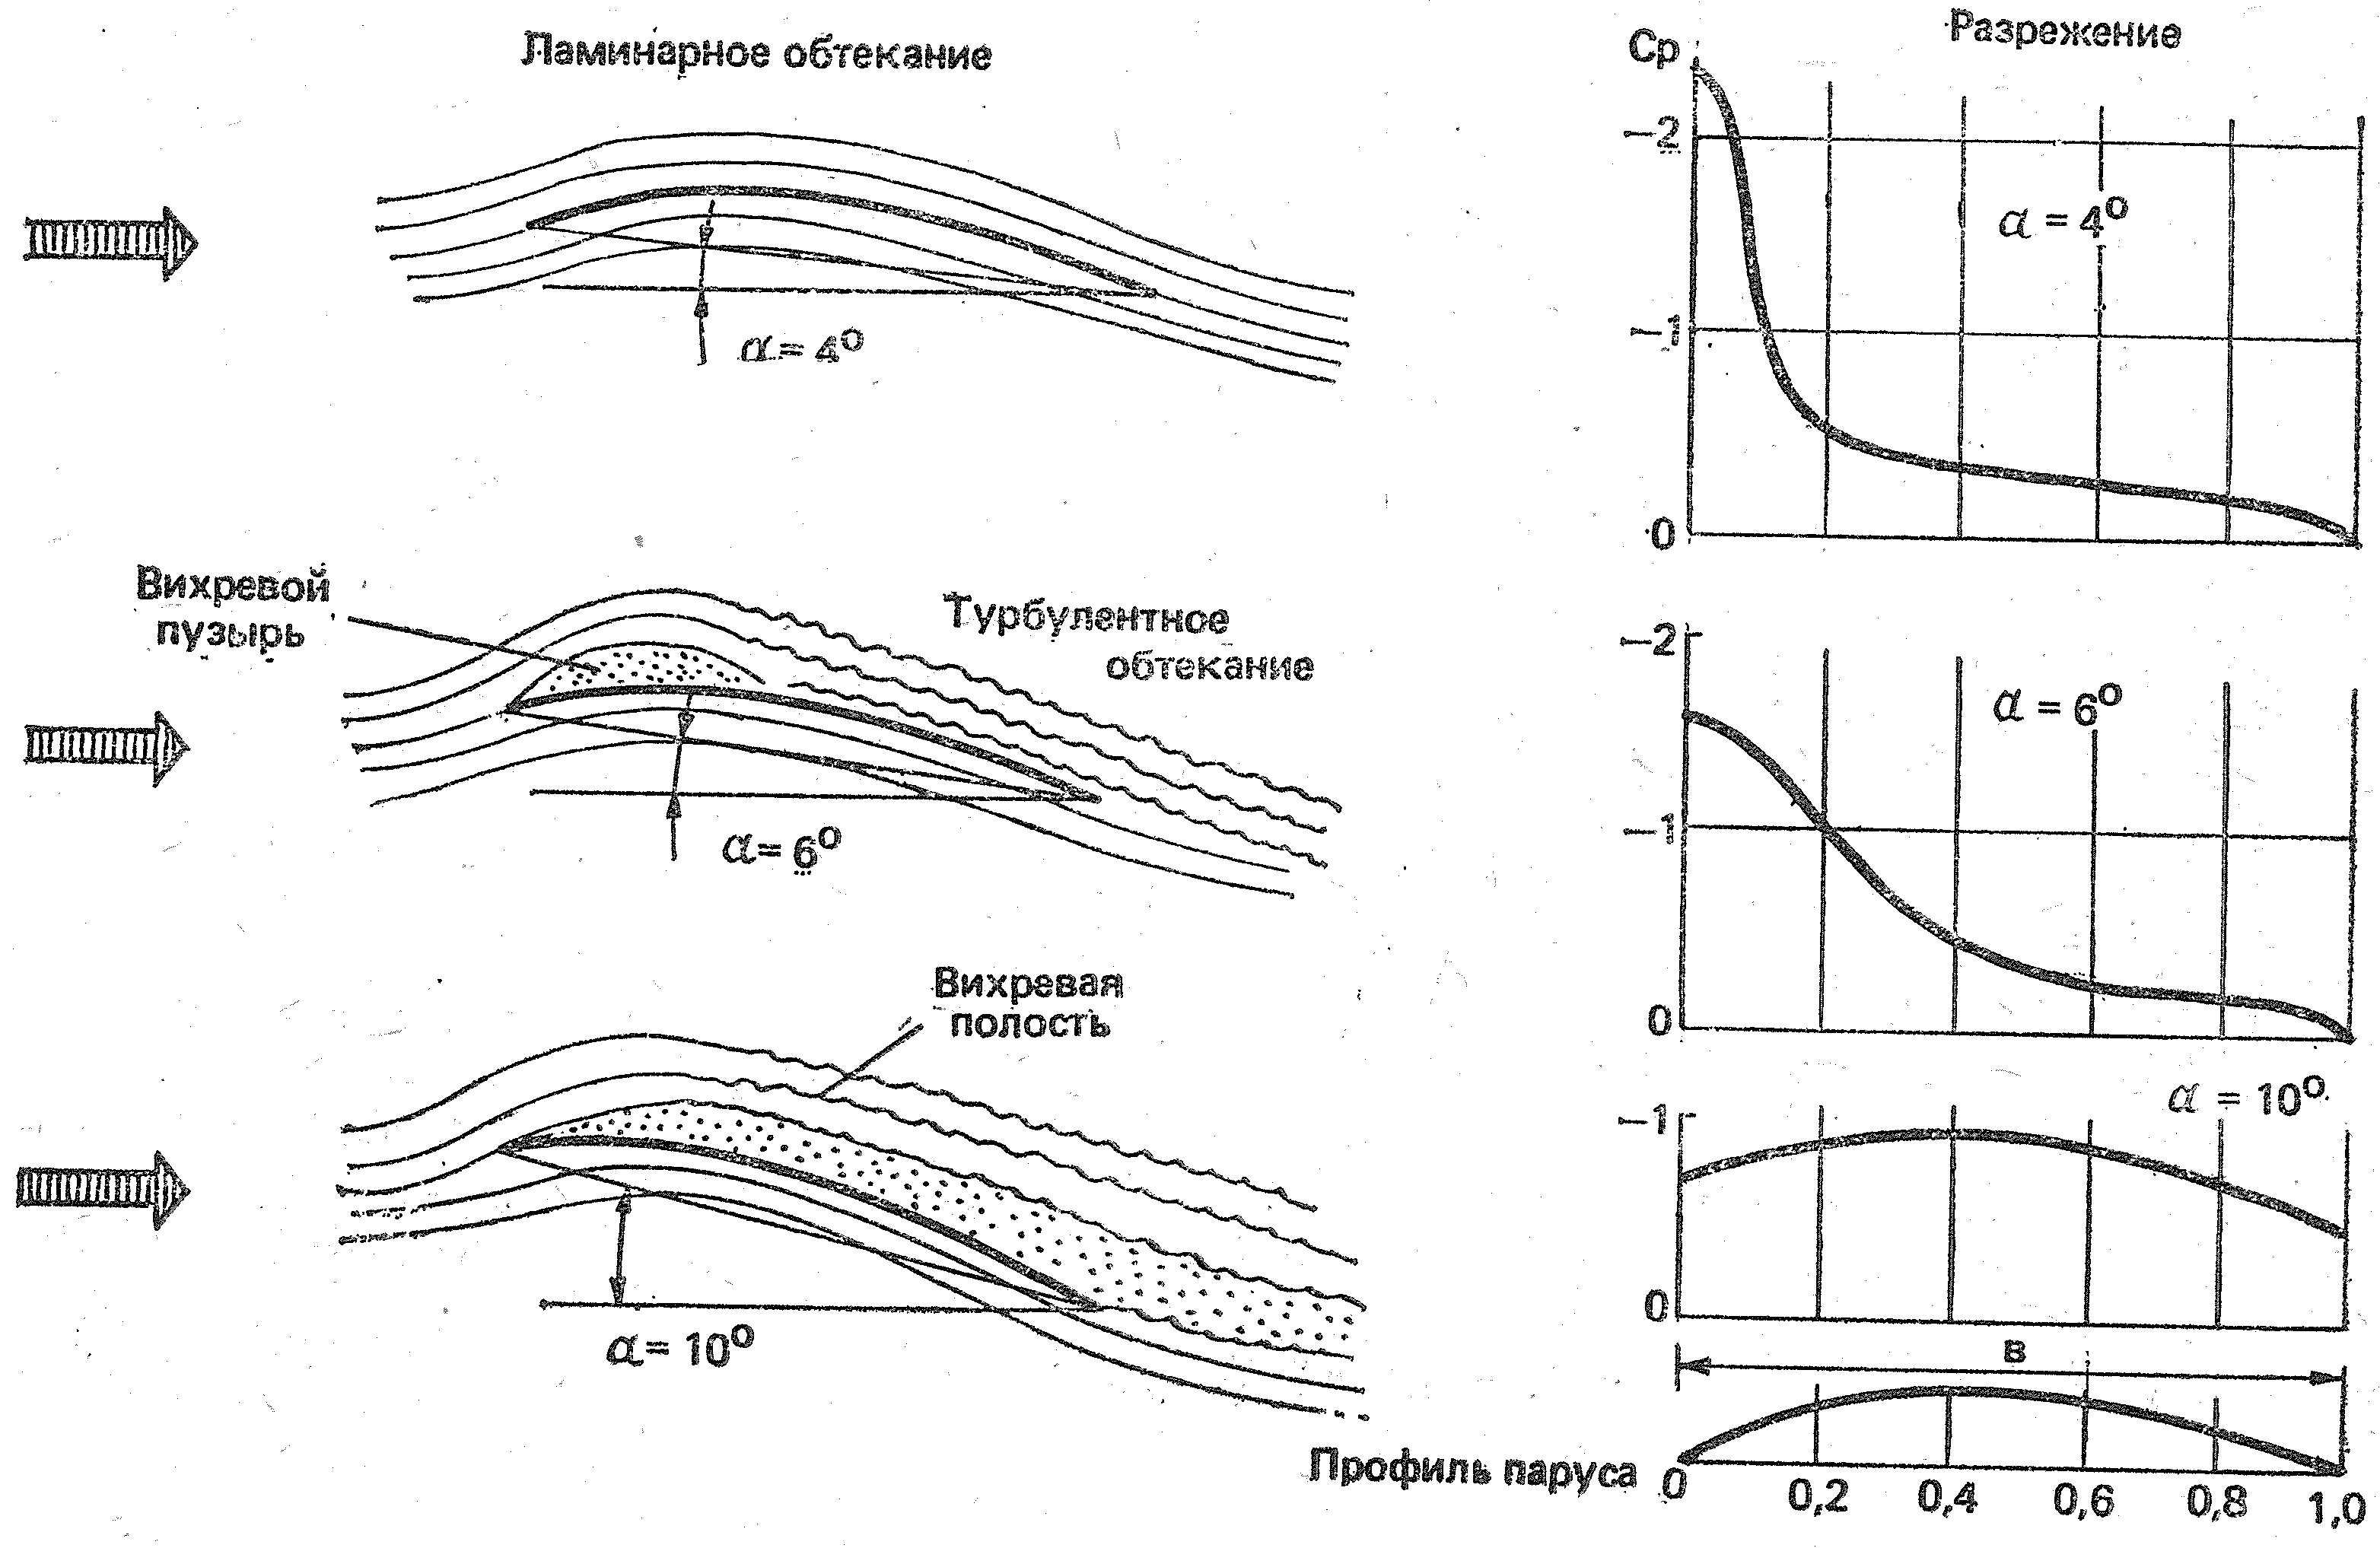
\includegraphics[scale=1.3]{0021P}
  \caption{Режим обтекания паруса и распределение пониженного давления (разрежения) по ширине профиля в зависимости от угла атаки $\alpha$}
  \label{fig:21}
\end{figure*}

Вихревой пузырь, размеры которого увеличиваются по мере увеличения угла атаки, вносит существенные изменения в распределение пониженного давления вдоль подветренной стороны паруса по сравнению с показанным на рис.~\ris{10} распределением давления на жестком профиле с толстой скругленной передней кромкой. Напомним, что именно разрежение на подветренной стороне паруса играет основную роль в создании подъемной силы и, следовательно, силы тяги на острых к ветру курсах. 

На рис.~\ris{21} представлены результаты замеров разрежения на жестком выпукло-вогнутом профиле, аналогично парусу. На малых углах атаки профиль обтекается плавным ламинарным потоком. 

При $\alpha = 4\gr$ начинаете отрыв пограничного слоя. В этот момент достигается наивысшее разрежение, пик которого расположен вблизи входящей кромки.
 
При $\alpha = 6\gr$ вихревой пузырь занимает на подветренной стороне около 25\,\% хорды профиля $b$. Разрежение уменьшается, и эпюра его становится более плавной. 

При $\alpha = 10\gr$ пузырь охватывает всю ширину профиля, его толщина составляет 3,5\,\% $b$. Давление повышается в 2,5 раза по сравнению с разрежением при $\alpha = 4\gr$; пика разрежения практически нет \--- оно равномерно распределено по всей ширине профиля. Значит, подъемная сила существенно снизилась, а лобовое сопротивление возросло (см. рис.~\ris{27}). 

Таким образом, на курсе бейдевинд увеличение угла атаки паруса к вымпельному ветру более 5\otdo 6\gr нежелательно. На реальном парусе вихревой пузырь представляет собой невидимый глазу цилиндрический валик, распространяющийся по всей высоте паруса. Чем больше выбран шкот, тем большая часть подветренной поверхности паруса захватывается вихревым валиком, уменьшая подъемную силу. 

Для выбора оптимального угла атаки в последние годы используются индикаторы обтекания в виде ленточек из тонкой ткани, закрепленных на определенном расстоянии от передней шкаторины с обеих сторон паруса (рис.~\ris{22}).

\begin{figure*}[htb]
  \centering
  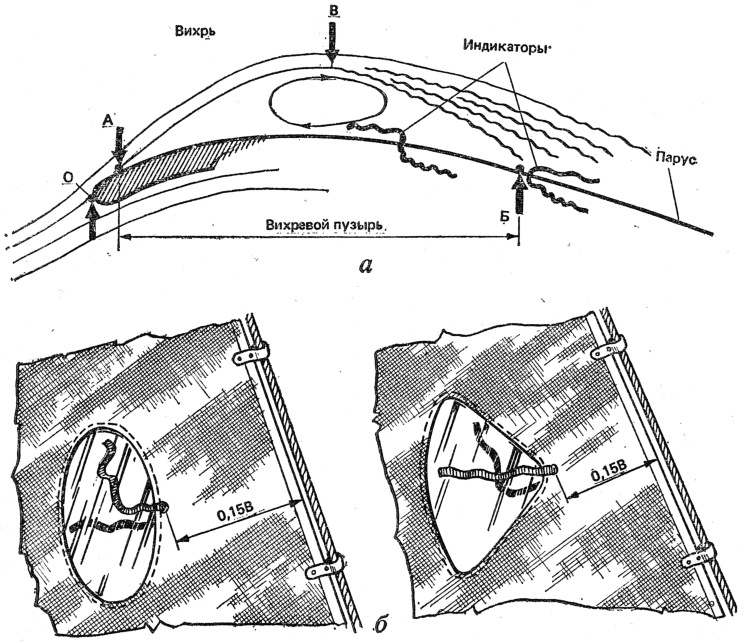
\includegraphics[scale=1.3]{0022P}
  \caption{Принцип работы (\textit{а}) и установка индикаторов обтекания на стакселе (\textit{б})}
  \label{fig:22}
  \small
  \centering{}
  О \--- критическая точка; А \--- точка отрыва пограничного слоя; Б \--- точка возврата пограничного слоя; В \--- переход ламинарного режима потока в турбулентный
\end{figure*}

Таким местом является точка Б возвpaтa пограничного слоя к поверхности паруса. При угле атаки $\alpha = 5\gr$ она отстоит от передней шкаторины примерно на 15\,\% ширины паруса в каждом его поперечном сечении. Как только вихревой пузырь достигнет этой точки, ленточка индикатора на подветренной поверхности паруса, ранее направленная назад по потоку воздуха, отклонится вверх и вперед, указывая на возникновение здесь вихрей. Дальнейшее выбирание шкотов \--- увеличение угла атаки \--- не только бесполезно, но даже вредно, так как приводит к большой потере подъемной силы.

Установка трех\-/четырех подобных индикаторов, равномерно распределенных по высоте стакселя, облегчает рулевому правильный выбор курса при лавировке. Выбрав наивыгоднейшим образом шкоты для данного курса, ведут яхту таким образом, чтобы индикаторы на наветренной стороне стакселя слегка подрагивали, а на подветренной были вытянуты в сторону задней шкаторины (рис.~\ris{23}).
 
Причиной падения подъемной силы на парусе является срыв потока с его подветренной стороны при увеличении угла атаки (что соответствует подбиранию шкотов или уваливанию яхты), поэтому главную роль играют индикаторы, расположенные на подветренной стороне. Если они начинают подниматься и совершать беспорядочные движения, значит, необходимо привести яхту к ветру или потравить шкоты.

Угол атаки, при котором подъемная сила перестает расти, называется критическим углом атаки. Его величина зависит от глубины и формы <<пуза>> паруса, аэродинамического удлинения $\lambda$ (оно для парусов вычисляется так же, как и для килей и рулей), наличия у передней шкаторины мачты или обтекателя штага.

\begin{figure*}[htb]
  \centering
  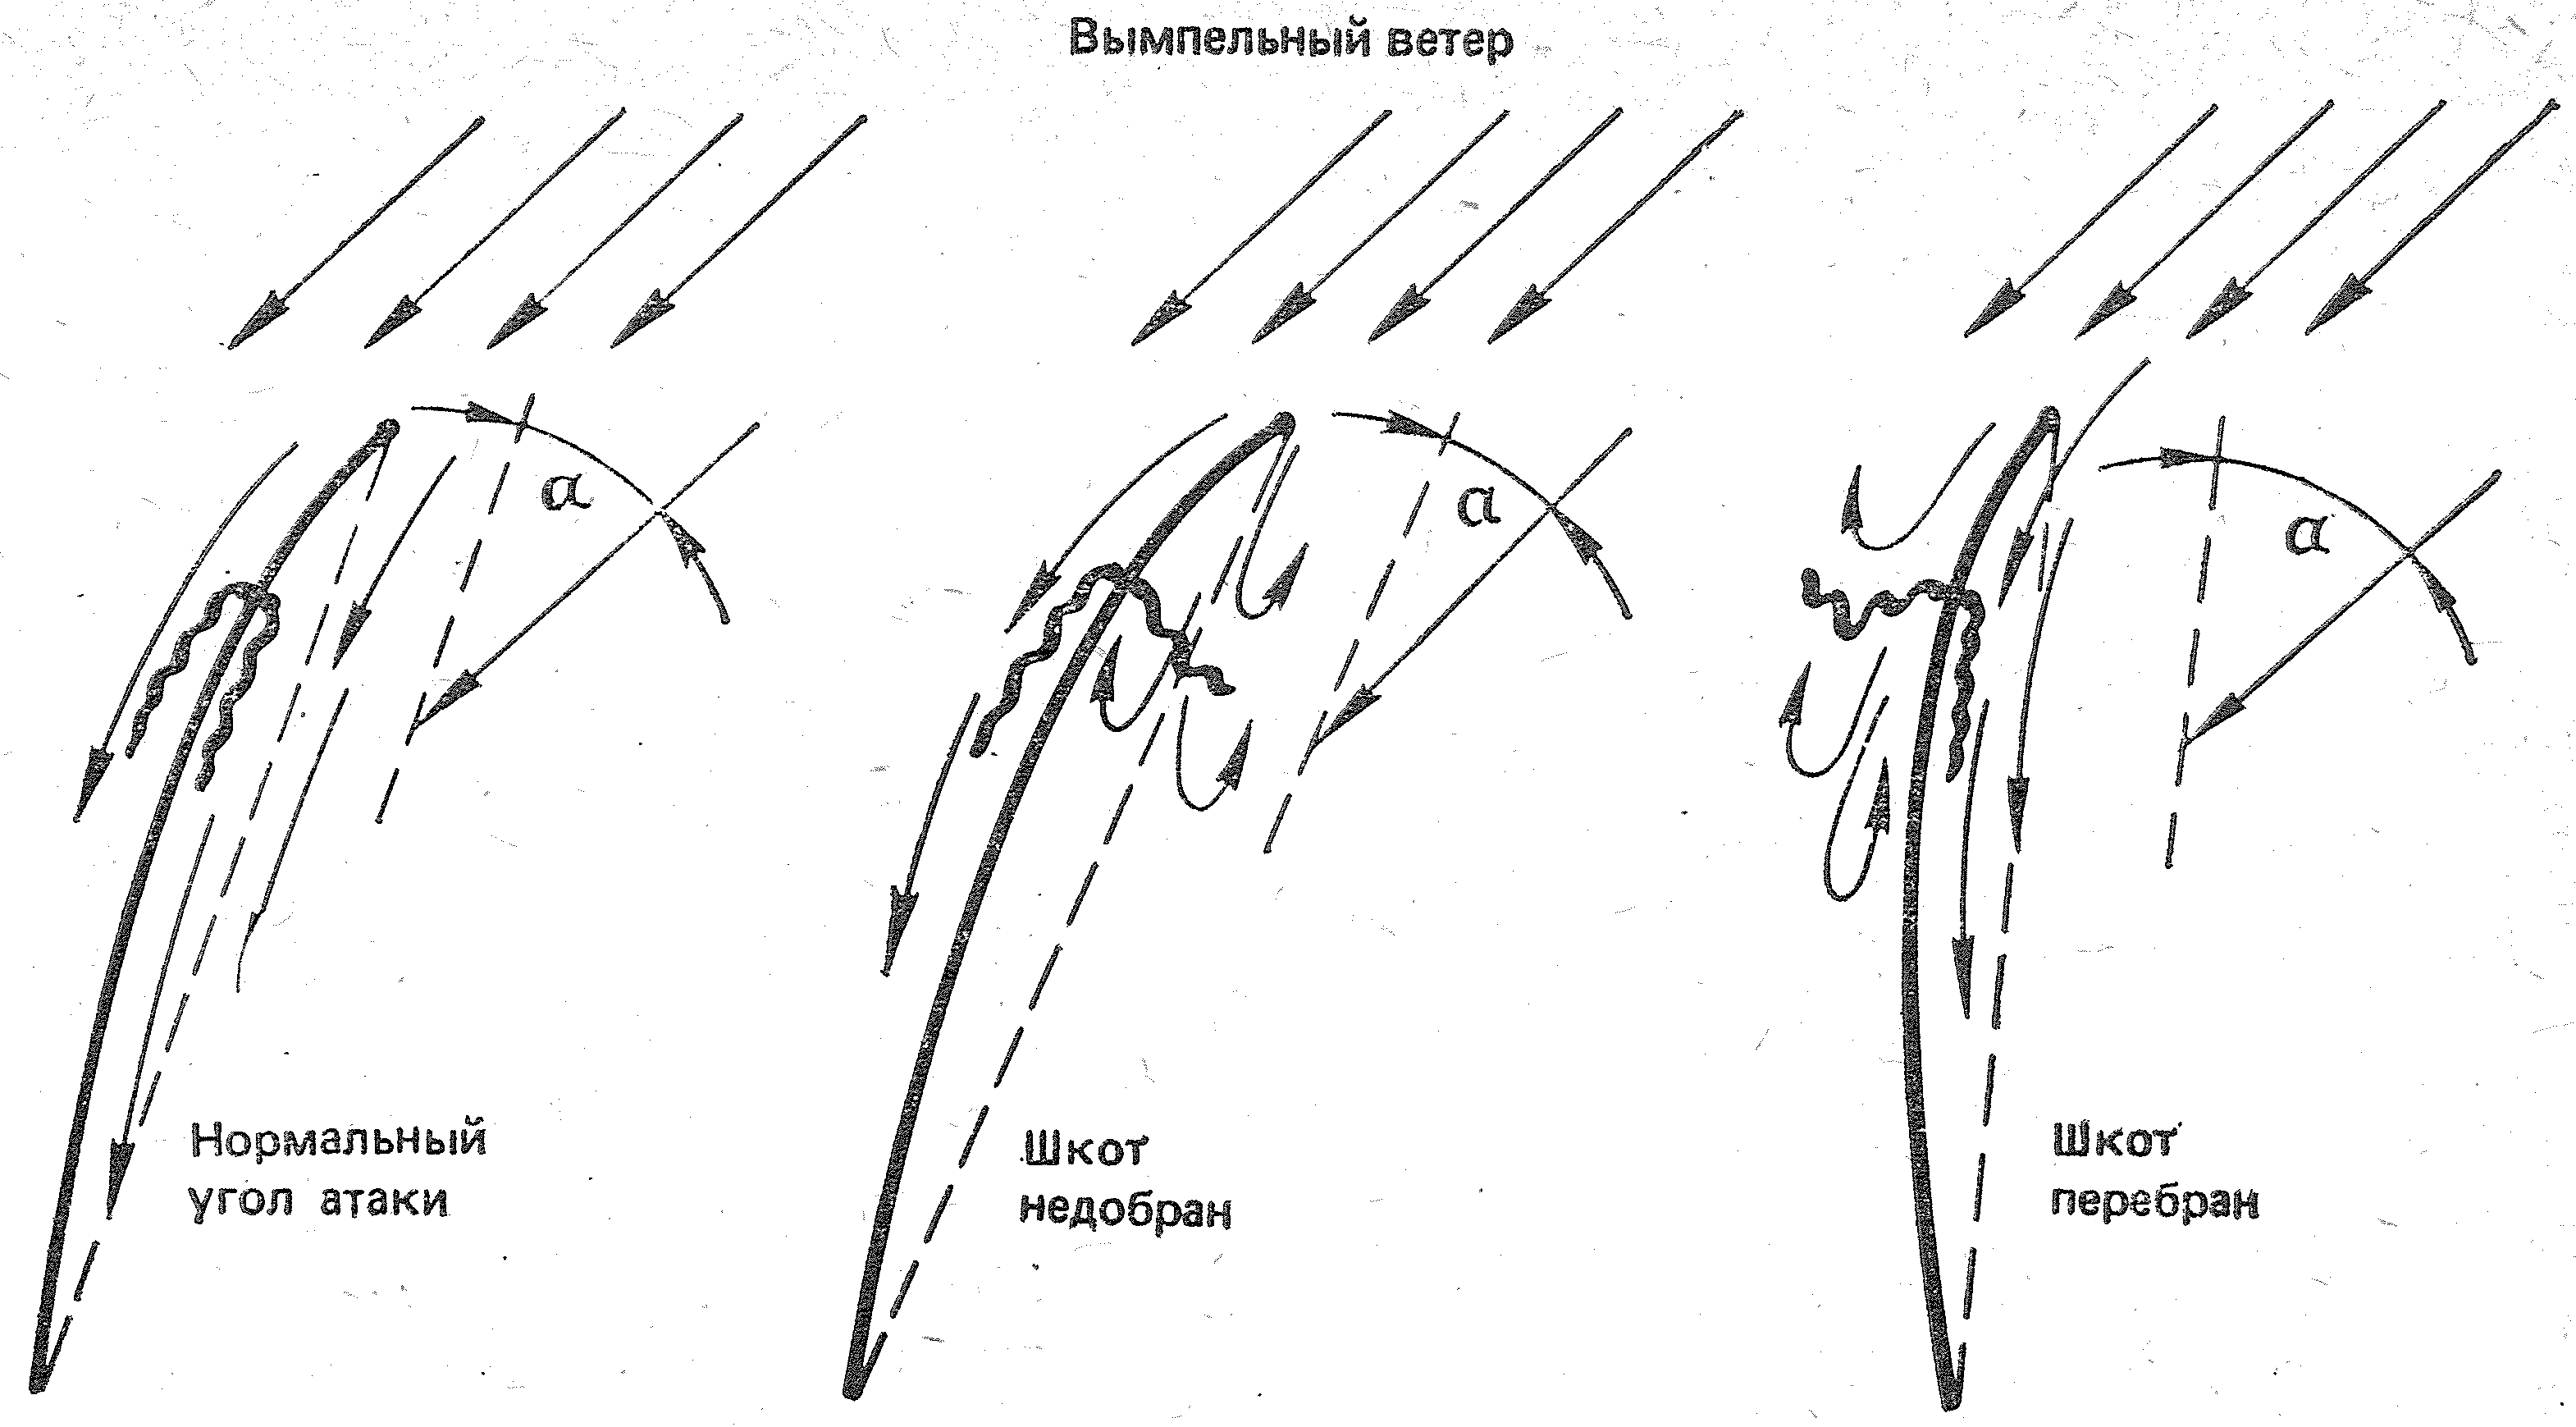
\includegraphics[scale=1.3]{0023P}
  \caption{Поведение индикаторов в зависимости от угла атаки паруса}
  \label{fig:23}
\end{figure*}

В слабый ветер поток воздуха происходит при меньших углах атаки, чем в сильный. При постановке стакселя перед гротом благодаря повышению скорости потока в зазоре между обоими парусами момент срыва сдвигается в сторону больших углов атак. Обратное действие оказывает мачта, срывающиеся с нее на подветренную сторону паруса вихри способствую срыву потока при меньших угла атаки. 

При увеличении угла атаки сверх критического подъемная сила падает, одновременно растет лобовое сопротивление. При $\alpha = 90\gr$ подъемная сила на парусе не создается: он обладает лишь лобовым сопротивлением.

\textbf{Поляра паруса.} Характеристикой аэродинамических качеств паруса является поляра \--- график изменения подъемной силы в зависимости от лобового сопротивления и угла атаки (рис.~\ris{24}, \textit{а}). Для того чтобы поляру можно было применить к парусу любых размеров, по осям координат откладывают не значения сил, а безразмерные коэффициенты подъемной силы \cidx{C}{Y} и лобового сопротивления \cidx{C}{X}. Данные для построения поляры получают в результате продувок моделей парусов в аэродинамических трубах. 

\begin{figure}[htb]
  \centering
  \includegraphics[scale=1.2]{0024P}
  \caption{Поляра паруса (\textit{а}) и силы, действующие на парус на курсе галфвинд (\textit{б})}
  \label{fig:24}
\end{figure}

С помощью поляры можно определить величины подъемной силы и лобового сопротивления, а также их составляющих \--- проекций на направление движения яхты. Опустив, например, из точки поляры, соответствующей углу атаки $\alpha = 20\gr$, перпендикуляр на ось движения яхты, можно найти величину коэффициента силы тяги \cidx{C}{Т} как отрезка прямой \cidx{А}{О}. Длина самого перпендикуляра $AB$ будет не что иное, как коэффициент силы дрейфа \cidx{C}{d}. Умножив численные значения коэффициентов \cidx{C}{Т} и \cidx{С}{d} на площадь паруса $S$ и скоростной напор $(\rho v^2)/2$, можно получить величину соответствующих сил. 

Поляра паруса позволяет определить наивыгоднейший угол установки парусов на данном курсе по отношению к ветру. Максимальная тяга, очевидно, определяется перпендикуляром к оси движения яхты, который одновременно является касательной к поляре. Угол атаки $\alpha = 14\gr$, определяемый точкой касания $C$, будет в данном случае наивыгоднейшим. Соответствующий ему угол установки паруса относительно \textit{ДП} яхты $\delta$ несложно найти, вычтя из курсового угла (по отношению к вымпельному ветру $\beta$ дрейф $\lambda$) и угол атаки $\alpha$ (см. рис.~\ris{19}).

Несложно выполнить аналогичные построения для различных значений курсового угла $\beta$ и определить наивыгоднейшие углы установки паруса и соответствующие им углы атаки. Можно убедиться, что для данного паруса почти на всех острых углах к ветру, вплоть до бакштага, наивыгоднейшие углы атаки близки и находятся в пределах 14\otdo 15\gr.

\textbf{Скручивание паруса.} С выбором оптимального угла атаки паруса связано его свойство скручиваться, т.\=,е. изменять угол атаки по высоте. При выбирании шкотов удается контролировать только нижнюю треть паруса; в верхней же части ткань имеет возможность несколько отклоняться на подветер, уменьшая тем самым угол атаки. Если не предусмотреть специальных средств для контроля скручивания паруса, то разность в углах атаки или угол скручивания может достичь 20\gr. А так как парус выбирают, ориентируясь на поведение его верхней части (пока не перестанет заполаскивать ткань у передней шкаторины), то нижняя часть оказывается работающей с избыточными углами атаки. Здесь может произойти срыв потока с подветренной стороны и соответственно упасть подъемная сила. Следовательно, тяга скрученного паруса оказывается ниже, чем если бы каждое его сечение по высоте имело оптимальный угол атаки. 

Особенно сильно заметно скручивание паруса на полных курсах и при свежем ветре, когда шкоты потравлены и нок гика задирается вверх. При этом верхняя часть паруса уходит под ветер и почти заполаскивает, а нижняя работает под слишком большим углом атаки. 

Для уменьшения скручивания грота на большинстве яхт применяют оттяжки гика, препятствующие задиранию нока вверх, а также проводку гика\-/шкота с одним или двумя поперечными погонами, простирающимися на всю ширину яхты. При мещении ползуна гика\-/шкота к борту яхты тяга шкотов становится почти вертикальной, благодаря чему удается держать заднюю шкаторину паруса на острых курсах более тугой. 

Свидетельством правильной регулировки натяжения оттяжки гика может служить одновременное (по всей высоте) заполаскивание ткани у передней шкаторины при потравливании шкота.

Было бы ошибкой считать, что парус вообще не должен иметь скручивания по высоте, т. е. иметь все сечения повернутыми относительно гика на один и тот же угол. На крупных яхтах надо учитывать изменение скорости и направления вымпельного ветра по высоте и наличие в верхней части паруса перетекания воздуха из зоны повышенного давления на подветренную сторону. В зависимости от высоты парусности и скорости ветра получается разность в углах атаки от 3\otdo 5\gr в бейдевинд до 10\otdo 12\gr на курсе бакштаг. В таких пределах скручивание паруса допустимо и способствует более эффективной его работе. 

Циркуляция воздуха вокруг крыла (см. рис.~\ris{10}), появляющаяся вместе с аэродинамической силой, вызывает незначительные по скорости поперечные потоки воздуха \cidx{V}{И} у входящей и выходящей кромок. Вследствие перетекания воздуха через кромки у концов крыла эти потоки усиливаются и отклоняют основной поток, набегающий на крыло, так, что угол атаки жесткого треугольного бермудского паруса по мере приближения к вершине увеличивается и близ фалового угла примерно на 20\,\% превышает угол атаки средней части паруса. Близ гика фактический угол атаки, наоборот, несколько уменьшается.

Таким образом, если бы парус не имел скручивания, то его верхняя часть работала бы при закритических углах атаки и практически не участвовала бы в создании движущей силы. Опытный экипаж постоянно контролирует и регулирует скручивание паруса в зависимости от силы ветра и курса яхты с помощью оттяжки гика и перемещения нижнего блока гика\-/шкота по погону.

\textbf{Влияние мачты.} Мачта является источником образования завихрений, которые особенно неблагоприятно сказываются на формировании потока на подветренной стороне паруса. Здесь вихревой след мачты уменьшает разрежение, вследствие чего уменьшается величина подъемной силы. Кроме того, сама мачта обладает достаточно большим лобовым сопротивлением. 

\begin{figure}[htb]
  \centering
  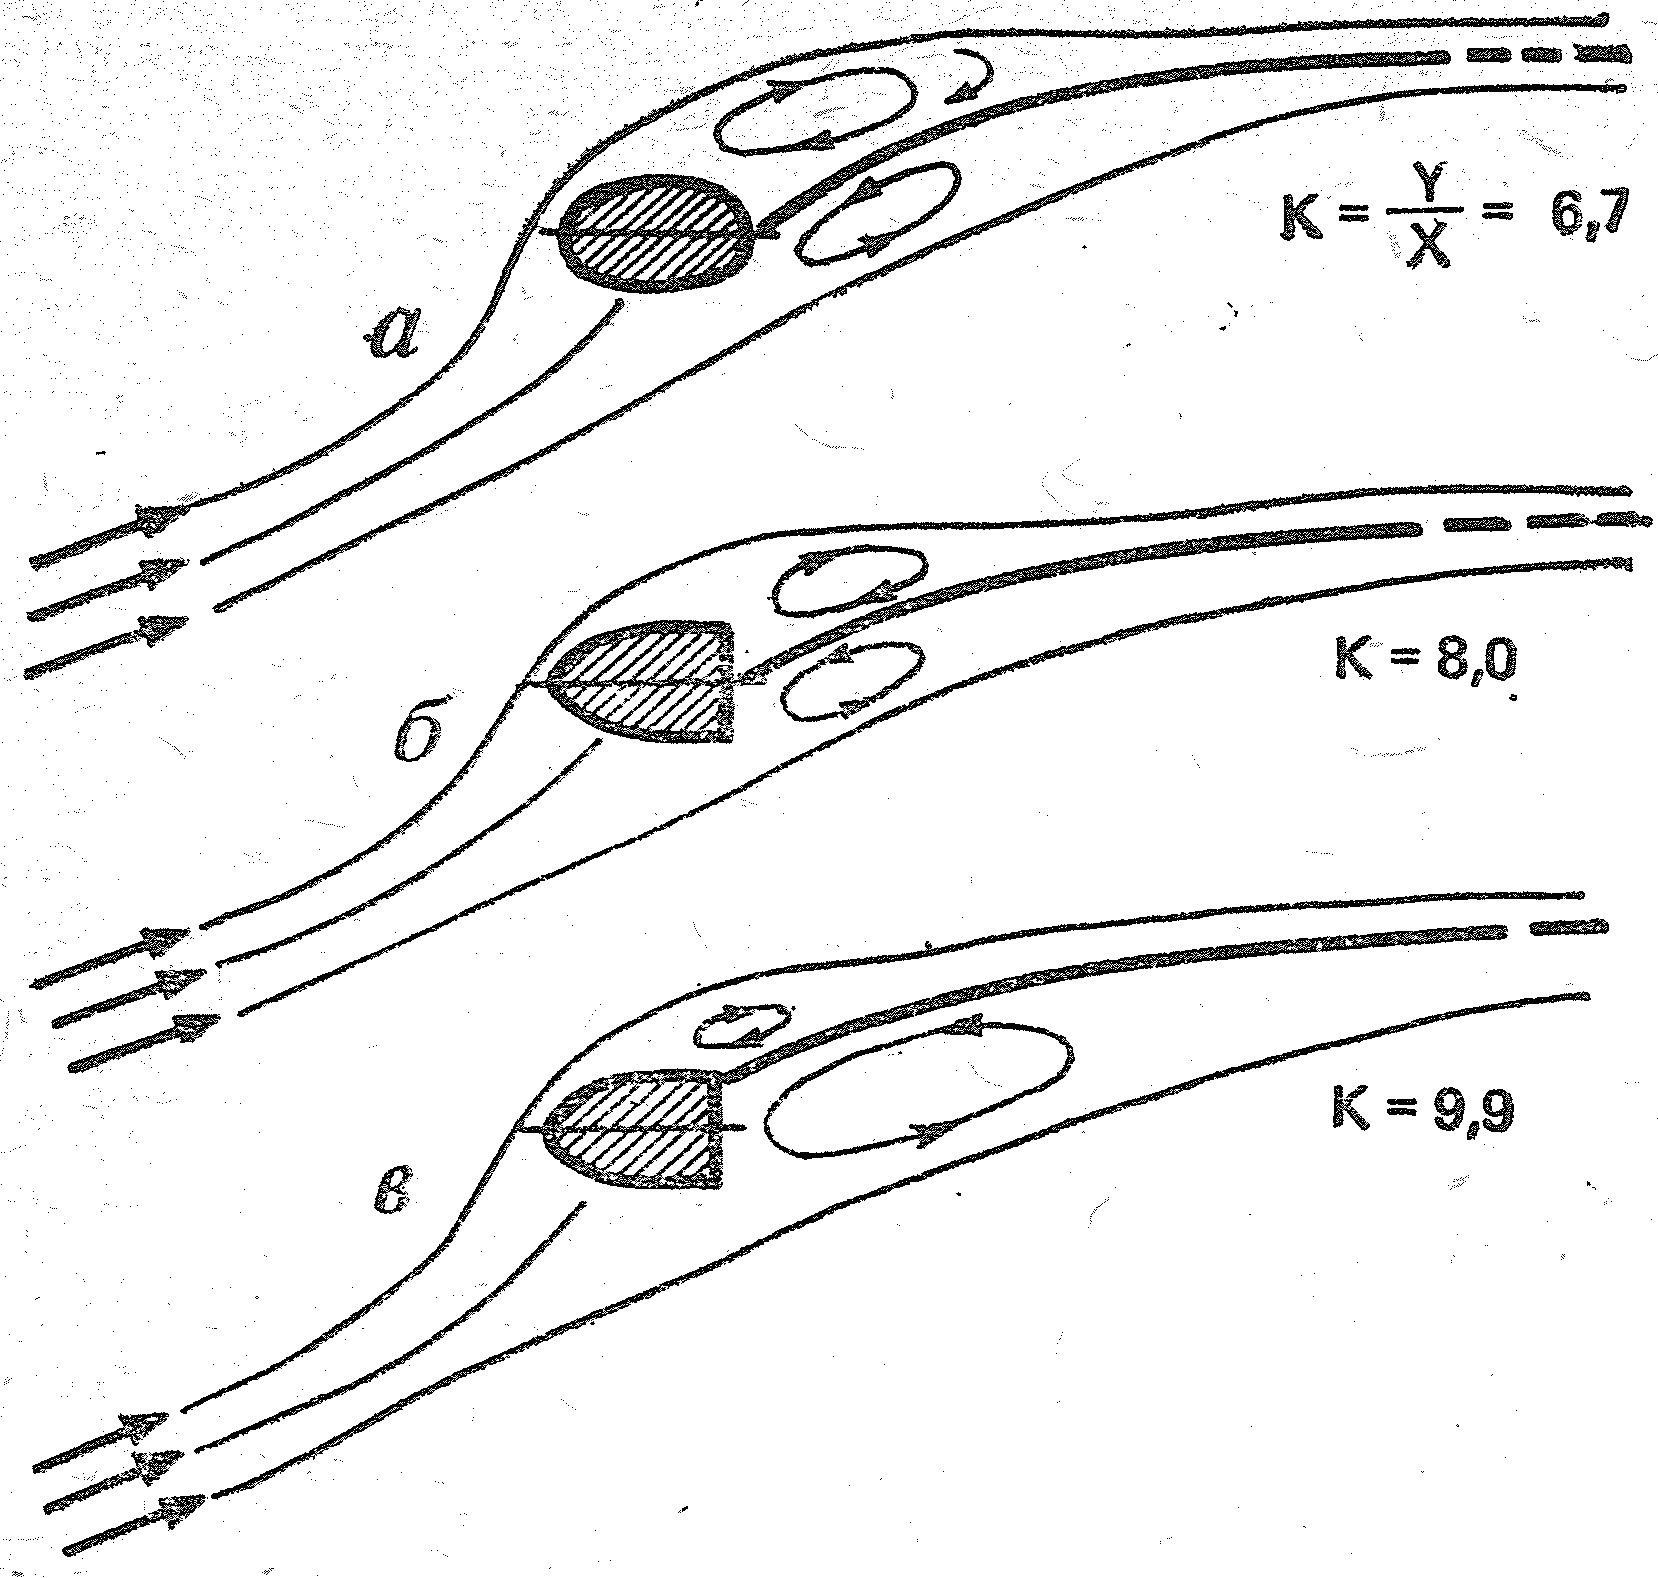
\includegraphics[scale=1.2]{0025P}
  \caption{Характер обтекания мачт}
  \label{fig:25}
  \small
  \centering{}
  \textit{а} \--- с эллиптическим поперечным сечением; \textit{б} \--- с параболической передней кромкой; \textit{в} \--- с парусом поставленным по подветренной кромке
\end{figure}

Большую роль играет форма поперечного сечения мачты, особенно передней ее кромки, на которой формируется поток. Важно, чтобы на курсе бейдевинд, когда яхта идет под углом 25\otdo 30\gr к вымпельному ветру, вихревая дорожка, срывающаяся с подветренной стороны мачты, имела бы минимальную ширину. Парус за мачтой параболическим поперечным сечение и тупой кормовой кромкой обладает более высоким аэродинамическим качеством, чем за мачтой эллиптического сечения (рис.~\ris{25}). Наиболее оптимальным оказывается вариант мачты с парусом, закрепленным передней шкаториной близ ее подветренной стороны: качество его работы на 40\,\% выше, чем паруса с эллиптической мачтой. Это лишнее свидетельство тому, что отрицательное влияние мачты в основном распространяется на подветренную сторону паруса.

Мачта, имеющая большое поперечное сечение, может снизить подъемную силу паруса на 25\,\% по сравнению с парусом, поставленным на штаге. Особенно велики потери подъемной силы при постановке паруса на рельсе с ползунками, когда в щель между мачтой и парусом перетекает воздух с наветренной стороны паруса в область пика разрежения на подветренной стороне. Неудачны мачты цилиндрического сечения, без сужения к топу: в верхней части отношение диаметра мачты уменьшающейся здесь ширине пару становится велико. Может оказаться, что часть паруса близ фалового yгла вообще не будет участвовать в создании подъемной силы, а следовательно, и тяги на курсе бейдевинд.

Наибольшее распространение на яхтах получили мачты, имеющие овальное поперечное сечение, с соотношением около 3:2, обеспечивающее большую продольную жесткость. Каплевидные и другие типы обтекаемых профилей целесообразны только в том случае, если мачта вращается для установки под наивыгоднейшим углом к вымпельному ветру при перемене галса. Такими мачтами снабжают обычно буepa и катамараны.

\section{Форма паруса и контроль за нею}

\begin{figure}[htb]
  \centering
  \includegraphics[scale=1.2]{0026P}
  \caption{Влияние <<пуза>> паруса на величину подъемной силы и лобового сопротивления}
  \label{fig:26}
\end{figure}

\textbf{Поперечный профиль паруса.} Основным фактором, влияющим на величину аэродинамических сил на парусе и его тяговые характеристики, является его профиль, т.\=,е. форма и размеры <<пуза>>.

На рис.~\ris{26} представлены поляры четырех жестких моделей бермудских парусов, имеющих аэродинамическое удлинение $\lambda = 4$ и расстояние максимальной глубины <<пуза>> от передней шкаторины, равное 1/3 хорды. От реальных парусов модели отличались еще отсутствием угла скручивания и постоянством относительной глубины <<пуза>> по высоте.

На полярах (рис.~\ris{26}) видно, что с уменьшением глубины <<пуза>> качество паруса возрастает благодаря снижению коэффициента лобового сопротивления (показано горизонтальной стрелкой). Максимальная подъемная сила паруса, наоборот, увеличивается по мере увеличения глубины <<пуза>> (показано наклонной стрелкой).

Посмотрим теперь, каким образом могут быть реализованы качества парусов в зависимости от их профиля. Предположим, что яхта идет курсом бейдевинд под углом $\beta = 30\gr$ к направлению вымпельного ветра. Очевидно, наибольшую тягу даст тот парус, касательная к поляре которого \--- перпендикуляр к линии пути яхты (см. рис.~\ris{24}) будет отстоять от точки 0 дальше подобных же касательных к другим полярам. В данном случае наибольшую тягу имеет парус с относительной глубиной <<пуза>> $f/b=1/10$. Однако нетрудно заметить, что выигрыш в тяге этого паруса будет минимальным по сравнению с более плоским парусом, имеющим $f/b = 1/15$. В то же время, более <<пузатый>> парус ($f/b = 1/10$) дает значительно большую поперечную силу дрейфа, чем парус с $f/b = 1/15$. Поэтому небольшое преимущество более <<пузатого>> паруса может быть реализовано на лавировке только в слабый ветер, когда абсолютная величина силы дрейфа будет невелика. В свежий ветер плавание с таким парусом сопровождается большим креном и соответственно дополнительным сопротивлением движению, так что в конечном счете выигрыша в скорости не получится. 

Еще более <<пузатые>> паруса $f/b=1/5$ и $f/b=1/4$ на курсе бейдевинд не только не дают увеличения силы тяги, но и отличаются намного большей величиной силы дрейфа. Однако более высокий коэффициент подъемной силы <<пузатых>> парусов может быть реализован на других, более полных, курсах по отношению к ветру: например, на курсе галфвинд, когда подъемная сила дает наибольшую составляющую на направление движения (см. рис.~\ris{24}, \textit{б}). В практике морских гонок это качество <<пузатых>> парусов используется благодаря смене на полных курсах лавировочных передних парусов на дрифтергеную, блупер или спинакер.

Следует заметить, что преимущества <<пузатых>> парусов могут быть использованы в основном при слабых ветрах, когда скорость яхты прямо пропорциональна силе тяги. В сильные ветра, когда яхта развивает свою предельную скорость под обычными лавировочными парусами и дальнейшее повышение тяги практически не увеличивает скорость, постановка <<пузатых>> парусов не дает эффекта. Более того, большая сила дрейфа <<пузатого>> паруса обусловливает больший крен и дрейф и соответствующее повышение сопротивления воды движению яхты. 

В качестве основных (лавировочных) парусов для среднего ветра (2\otdo 4 балла) применяют паруса с <<пузом>> $f/b=9\motdo 10\,\%$. Для слабого ветра выгодны более <<пузатые>> паруса \--- $f/b$ до 12\,\%, а при ветре более 5 баллов \--- паруса с <<пузом>> не более 6\,\% ($f/b=1/17\motdo 1/25$). 

В гонках яхтсмены широко пользуются различными способами регулирования величины <<пуза>> парусов в зависимости от силы ветра. Особенно это относится к настройке грота, так как по правилам IOR замена его во время гонок не допускается, а ветровые условия могут изменяться в довольно широких пределах. Основными средствами регулирования <<пуза>> грота являются продольный изгиб мачты, натяжение шкаторин (оттяжка Кэнингхэма и грота\-/шкот), уплощающий риф, натяжение гика\-/шкота и положение его блока на погоне по ширине яхты, оттяжка гика. Продольный изгиб мачты позволяет контролировать две верхние трети паруса, в то время как другие средства эффективны при изменении профиля у гика.

В слабый ветер, когда важно иметь грот наиболее <<пузатым>>, мачта должна быть прямой, грота\-/шкот и оттяжку гика выбирают не до конца, оттяжка Кэнингхэма растравлена. Блок на погоне гика\-/шкота перемещают от \textit{ДП} в сторону наветренного борта; гика\-/шкот втугую не выбирают.

Для увеличения <<пуза>> стакселя или генуи блок (кипу) стаксель\-/шкота перемещают вперед и ближе к \textit{ДП} яхты. При этом <<пузо>> перемещается вперед, натяжение задней шкаторины ослабляется, зазор между гротом и стакселем увеличивается. 

С усилением ветра мачте придают изгиб с выпуклостью, направленной вперед, увеличивая натяжение ахтерштага (при оснастке типа 3/4 или 7/8) или регулируя натяжение промежуточного штага и бакштагов (при топовой оснастке). Благодаря этому излишек паруса убирается в образовавшийся серп у передней шкаторины, <<пузо>> становится меньше и перемещается ближе к мачте. Оттяжку Кэнингхэма, грота\-/шкот и оттяжку гика выбираю втугую; блок гика\-/шкота смещают по погону на подветренный борт. Шкоты выбирают более туго, чем в слабый ветер. При необходимости сделать парус еще более плоским в нижней части берут уплощающий риф, используя люверсы, расположенные вблизи гика.

Профиль генуи может быть сделан более плоским при передвижении блока стаксель\-/шкота назад и к борту большем натяжении передней шкаторины. Значительное влияние на профиль передних парусов оказывает натяжение штага: для того чтобы парус стал более плоским, необходимо по возможности ликвидировать прогиб штага.

Большое влияние на тяговые характеристики паруса кроме величины <<пуза>> оказывает место положения максимальной выпуклости от передней шкаторины. На рис.~\ris{27} показано распределение разрежения на подветренной стороне жесткой модели паруса с относительной величиной <<пуза>> $f/b = 0,188$ при отстоянии максимального <<пуза>> на 40 и 60\,\% хорды от передней кромки и при угле атаки $\alpha = 15\gr$ (характерный <<провал>> на эпюре давления являйся следствием развитого вихревого пузыря \--- см. рис.~\ris{21}). Как видим, в создании движущей силы главную роль играет передняя часть паруса, где концентрируется разрежение у паруса с <<пузом>>, расположенным на 40\,\% хорды от передней шкаторины. Когда же <<пузо>> смещено к задней шкаторине, область разрежения охватывает и заднюю часть профиля, вследствие чего увеличивается составляющая \ve R, направленная против движения яхты. Таким образом, при смещении <<пуза>> к задней шкаторине эффективность паруса снижается как в результате падения подъемной силы в передней части паруса, так и в результате роста сил сопротивления, тормозящих ход судна.

\begin{figure}[htb]
  \centering
  \includegraphics[scale=1.2]{0027P}
  \caption{Эффект распределения разрежения на подветренной стороне паруса на результирующую аэродинамическую силу на парусе}
  \label{fig:27}
  \small
  \centering{}
  \textit{а} \--- эпюра распределения разрежения; \textit{б} \--- силы на парусе; \textit{1} \--- парус с максимальным <<пузом>>, расположенным на растоянии $0,4 b$ от передней шкаторины; \textit{2} \--- парус с <<пузом>>, расположеным на $0,6 b$ от передней шкаторины. $ve Y_1$ и $\ve Y_2$ \--- подъемна сила; \ve T и \ve R \--- составляющие силы \ve A по направлению ветра
\end{figure}

Лавировочные паруса шьют с максимальной глубиной <<пуза>>, расположенной от передней шкаторины на расстоянии от 35\otdo 40\,\% ширины паруса $b$ для плоских парусов, до 40\otdo 50\,\% $b$ для более полных.

Во всех поперечных сечениях максимальная глубина <<пуза>> должна находиться в указанных пределах. Поэтому по мере увеличения ширины паруса по направлению к гику соответственно увеличивается и абсолютная величина <<пуза>>. У гика на обезветренном парусе <<пузо>> образует <<мешочек>>, который в сильный ветер можно убрать в скатку уплощающего рифа.

\textbf{Форма паруса.} С точки зрения аэродинамики крыла наиболее выгодным был бы парус с эллипсовидной верхней частью. Именно в его верхней части образуются потоки воздуха, перетекающего с наветренной стороны на подветренную \--- в область разрежения. В результате возникают вихри, срывающиеся с кромки паруса и уходящие в пространство. Эти возмущения требуют затрат кинетической энергии ветра, которые выражаются в росте общего аэродинамического сопротивления судна в виде составляющей индуктивного сопротивления. 

\begin{figure}[htb]
  \centering
  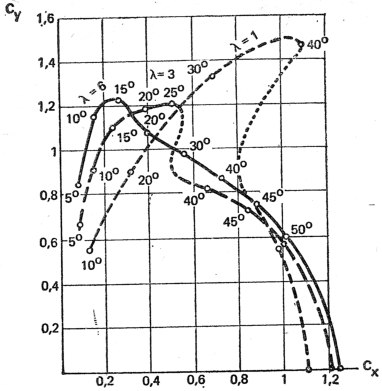
\includegraphics[scale=1.2]{0028P}
  \caption{Поляры парусов с различным аэродинамическим удлинением}
  \label{fig:28}
\end{figure}

Очевидно, что наибольшим индуктивным сопротивлением обладает четырехугольный гафельный парус, у которого перетекание воздуха происходит по верхней и нижней широким кромкам. Поэтому коэффициент подъемной силы здесь резко падает (см. рис.~\ris{8}).

У паруса с эллипсовидной верхней частью величина подъемной силы из-за плавного уменьшения площади паруса у верхнего конца также плавно убывает. Благодаря этому плавно убывает и интенсивность перетекания воздуха через кромки, не происходит местного изменения угла атаки и коэффициента подъемной силы. 

Попытка приблизить форму паруса к эллипсовидной при существующих ограничениях ширины фаловой доски и эластичности мачты была сделана, например, на английском двенадцатиметровике <<Лайонхат>> \--- претенденте на Кубок Америки 1980\,г.: верхняя часть мачты на нем была сильно изогнута. Испытания в аэродинамической трубе показали, что грот с гнутой мачтой дает примерно 10\otdo 30\,\% увеличения движущей силы по сравнению с обычным бермудским парусом или увеличение скорости лавировки на ветер порядка 4\,\%.
 
У треугольного паруса основная площадь и, следовательно, нагрузка сосредоточены в нижней трети. По мере приближения к фаловому углу площадь и подъемная сила убывают, что сопровождается соответствующим уменьшением скорости и фактического угла атаки паруса к набегающему потоку. Близ фалового угла также усиливается отрицательный эффект мачты поскольку размеры ее сечения увеличиваются относительно хорды паруса. Эксперименты показали, что если срезать бермудский парус на 15\,\% высоты от вершины, то практически его тяга не уменьшится. 

Существенное влияние на характеристики паруса оказывает аэродинамическое удлинение паруса (отношение длины передней шкаторины) к его средней хорде, измеренной на половине высоты, или отношение квадрата высоты паруса и его площади.

На рис.~\ris{28} представлены поляры трех парусов различного удлинения --- от $\lambda = 1$ до 6, имеющих одинаковое <<пузо>> $f/b=7,4\,\%$. Сравнивая поляры можно заметить, что при угле атаки $\alpha = 10\gr$ наивысшую аэродинамическу силу дает парус с максимальным удлинением $\lambda = 6$. Этот же парус имеет наивыгоднейшее направление аэродинамической силы для получения максимальной тяги на курсе бейдевинд. 

Аэродинамическая сила на парус имеющем $\lambda = 6$ достигает максимум при $\alpha = 15\gr$, затем падает. При угле атаки около 35\gr, т. е. на полных курсах, заметное преимущество получай более широкие паруса, имеющие $\lambda = 1$. Таким образом, можно сделать вывод, что парус с большим удлинением при переходе яхты на полный курс становится менее выгодным. На курсе полный бакштаг, например, более быстроходной может оказаться яхта, ocнащенная широкими гафельными парусами с удлинением около 1. Вот почему несмотря на общепризнанное преимущество бермудских парусов, гафельные паруса довольно часто применяют на моторно-парусных яхтах, у которых паруса используются преимущественно при сильных ветрах и на попутных курсах. 

У большинства современных яхт лавировочные паруса имеют отношение длин шкаторин от 3 до 5; паруса для полных курсов \--- дрифтеры, блуперы и спинакеры шьют с соотношением шкаторин, близким к 1.

Пределом для использования парусов большого удлинения является ограниченная остойчивость яхт, не позволяющая чрезмерно повышать положение \textit{ЦП}. Более высокая парусность требует также рангоута большего сечения, что приводит к распространению влияния мачты на большую часть площади грота.

\section{Взаимодействие парусов}

Мы рассматривали особенности \--- аэродинамики одиночного паруса как крыла с тонким поперечным профилем. Большинство яхт, однако, оснащены по крайней мере двумя парусами \--- гротом и стакселем. Поскольку оба паруса расположены в непосредственной близости друг от друга и обтекаются одним потоком воздуха, то естественно предположить наличие их взаимного влияния. 

\begin{figure}[htb]
  \centering
  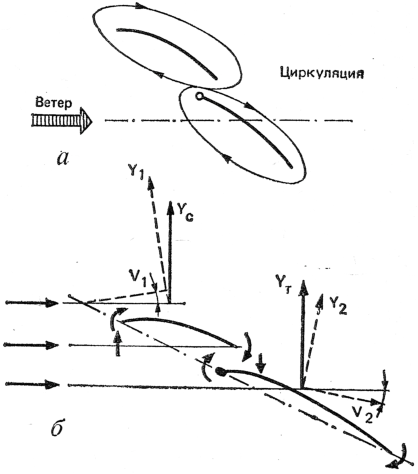
\includegraphics[scale=1.2]{0029P}
  \caption{Взаимодействие грота и стакселя}
  \label{fig:29}
  \small
  \centering{}
  \textit{а} \--- циркуляция потока вокруг обоих парусов; \textit{б} \--- влияние отклонения потока, натекающего на грот и стаксель под действием циркуляции; $\ve Y_C$ и $\ve Y_T$ \--- подъемные силы на стакселе и гроте, работающих как изолированные паруса; $\ve Y_1$ и $\ve Y_2$ \--- подъемные силы на парусах, работяющих совместно; $\ve V_1$ и $\ve V_2$ \--- скорости, вызванные циркуляцией потока вокруг обоих парусов
\end{figure}

До недавнего времени среди яхтсменов пользовалась популярностью теория Вентури, заимствованная из авиации. Согласно этой теории, основным назначением стакселя считалось создание щели \--- сопла между стакселем и гротом, входя в которую, поток воздуха увеличивает свою скорость, способствуя тем самым понижению давления на подветренной стороне грота, особенно в районе, где паруса перерывают друг друга. В результате должна увеличиваться аэродинамическая сила на гроте.

В настоящее время взаимодействие парусов рассматривается на основании вихревой теории крыла \--- исходя из наличия циркуляции вокруг обоих парусов (рис.~\ris{29}). Основная роль в паре грот \--- стаксель принадлежит стакселю. Бесспорно, что воздух, протекающий в щели между гротом и стакселем, имеет повышенную скорость. Однако это прежде всего сказывается на скорости потока, обтекающего подветренную сторону стакселя. Частицы воздуха, вырываясь из щели, увлекают с собой воздух с подветренной стороны стакселя подобно эжектору. Соответственно ускоряется поток вдоль всей подветренной поверхности стакселя, увеличивается циркуляция вокруг его профиля и возрастает аэродинамическая сила. И что еще важно - парус может работать без срыва потока на больших углах атаки.
 
Вызванная скорость (поперечная составляющая вследствие циркуляции) у передней шкаторины грота увеличивает угол атаки, под которым поток натекает на стаксель. Благодаря этому аэродинамическая сила растет и отклоняется вперед \--- на более выгодный угол. На курсе бейдевинд, к слову сказать, большой генуэзский стаксель дает на 30\,\% большую движущую силу, чем грот, и на 45\,\% меньшую силу дрейфа.
 
Грот работает в области потока, отклоняемого вызванными скоростями у задней шкаторины стакселя. Это приводит к уменьшению угла атаки грота. Однако воздух, отраженный от стакселя, как бы прилипает к подветренной поверхности грота, благодаря чему предотвращается отрыв от нее пограничного слоя.

Стаксель влияет и на положение критической точки: она перемещается с наветренной стороны мачты ближе к ее передней кромке. В результате уменьшается скорость потока с подветренной стороны грота и сильно снижается пик разрежения у передней шкаторины. Поэтому тенденция к отрыву пограничного слоя и образованию завихрений на гроте ослабевает, парус более эффективно работает на больших углах атаки, чем без стакселя. Скорее этим, а не ускорением потока в щели между гротом и стакселем, по теории Вентури, можно объяснить положительное действие стакселя на работу грота.

Чем больше выбирают стаксель, тем меньше становится разность давлений на подветренной и наветренной сторонах грота. Когда они сравняются, выпуклая форма паруса уже не может поддерживаться \--- парус заполаскивает. Поскольку стаксель более эффективен, чем грот, и дает меньшую кренящую силу, то экипажи крейсерско\-/гоночных яхт уделяют большое внимание подбору стакселей для различных курсов и силы ветра. В гонках при усилении ветра целесообразно уменьшат площадь парусности рифлением грота продолжая по возможности нести стаксель. На отдельных порывах крен можно уменьшать, потравливая грот.

Поскольку Правила обмера IOR прямо не ограничивают длину нижней шкаторины стакселей, то обычно стараются шить их с максимальным перекроем (заходом стакселя за мачту). Существуют, однако, вполне определенные пределы перекроя, далее которых парус теряет свою эффективность и начинает отрицательно влиять на работу грота.

Прежде всего это обеспечение оптимального угла установки стакселя относительно ДП яхты, который равен для лавировки 12\otdo 18\gr. Это труднодостижимо при большой длине нижней шкаторины стакселя и сравнительно небольшой ширине палубы яхты. Как правило, кипы стаксель\-/шкотов удается разместить при несколько меньших углах установки паруса \--- 9\otdo 12\gr. По этому при слишком <<пузатом>> стакселе возможен сток потока воздуха с него на переднюю шкаторину грота и заполаскивание ее по всей высоте. Кроме того, возможно сильное скручивание стакселя: в верхней части ветер будет выдувать из паруса и он перестанет работать. 

\begin{figure}[htb]
  \centering
  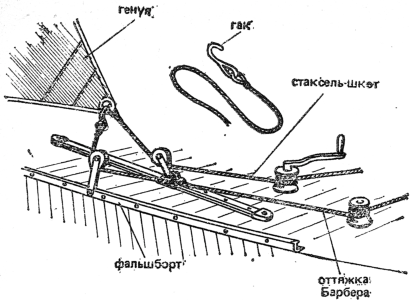
\includegraphics[scale=1.2]{0030P}
  \caption{Оттяжка шкотового угла стакселя}
  \label{fig:30}
\end{figure}

Для регулирования положения кип стаксель\-/шкотов в зависимости от величины стакселя и курса относительно ветра используют специальный фальшборт из металлического угло\-/бульбового профиля с большим числом отверстий или крепят кипы на передвижных ползунах, скользящих по прочному палубному рельсу. При настройке стакселя стараются получить равномерный зазор между гротом и стакселем по всей высоте и <<пузо>> стакселя, смещенное к передней шкаторине. При перемещении кипы вперед тяга шкота сильнее натягивает заднюю шкаторину. В результате <<пузо>> увеличивается по всей площади, парус меньше скручивается, но возможно заворачивание задней шкаторины на ветер. При перемещении кипы назад, увеличивается натяжение нижней шкаторины; натяжение задней шкаторины будет недостаточным, парус сильно скрутится и может заполаскивать в верхней части. Иногда полезно применить дополнительную снасть \--- оттяжку шкота (рис.~\ris{30}) для осаживания задней шкаторины. Выбрав втугую парус по нижней шкаторине за шкот, с помощью оттяжки добиваются нужного натяжения задней шкаторины и положения <<пуза>> по ширине паруса, устраняют сильное скручивание. Правильно отрегулированный стаксель должен давать поток воздуха, направленный по касательной к поверхности грота и при приведении яхты заполаскивать сразу по всей высоте. Хорошую службу при настройке могут оказать индикаторы (см. рис.~\ris{22}--\ris{23}).

Большое влияние на полноту стакселя оказывает прогиб штага. Чем сильнее при усилении ветра прогибается штаг, тем больше становится <<пузо>> паруса и он начинает задувать на грот. В известной мере прогиб компенсируется специальным раскроем стакселя с выпуклостью в нижней части передней шкаторины и вогнутостью (отрицательным серпом) в верхней. Многие яхты за рубежом снабжают мощными гидравлическими, винтовыми устройствами или талями для увеличения натяжения ахтерштага и даже наклона мачты назад.

\section{Лобовое сопротивление яхты}

Влияние лобового (воздушного) сопротивления яхты на ее ходовые качества исключительно велико. На курсе бейдевинд при ветре 4 балла на преодоление воздушного сопротивления яхты затрачивается около одной трети силы тяги, развиваемой парусами. Поэтому снижение лобового сопротивления так же важно, как и снижение сопротивления воды.

В общем балансе воздушного сопротивления на долю парусов и рангоута приходится 70\otdo 78\,\%, такелажа \--- 3\otdo 5\,\%, корпуса \--- 15\otdo 18\,\%, экипажа \--- 4\otdo 6\,\%. Поскольку основную роль играют паруса и рангоут, рассмотрим причины, обусловливающие появление на них сил сопротивления.

Воздушное сопротивление, как и сопротивление воды, считают возможным разделить на несколько компонентов. Для парусов их два: индуктивное сопротивление и сопротивление формы (или профильное). Как мы уже говорили, индуктивное сопротивление является неизбежным следствием действия на парусе аэродинамической подъемной силы. По мере роста скорости вымпельного ветра и соответственно величины подъемной силы растет и величина индуктивного сопротивления. В средний ветер в области оптимальных углов атаки паруса ($\alpha = 5\motdo 15\gr$) индуктивное сопротивление существенно выше сопротивления формы. Проявляется оно в виде двух вихревых дорожек, стекающих с нижней шкаторины и близ фалового угла паруса.
 
Основные факторы, влияющие на индуктивное сопротивление, \--- аэродинамическое удлинение и форма парусов, угол скручивания и распределение <<пуза>> по высоте паруса. Чем больше удлинение паруса (т.\=,е. чем меньше относительно высоты паруса длина нижней шкаторины и верхней части паруса, через которые происходит перетекание воздуха из зоны повышенного давления на сторону разрежения), чем ближе к форме эллипса форма верхней части паруса, тем меньше индуктивное сопротивление. От угла скручивания и величины <<пуза>> в верхней части паруса зависит величина подъемной силы и ее распределение на этом участке. У треугольного бермудского паруса в верхней части желательно получить большую подъемную силу на единицу площади, чем на середине высоты мачты, потому что тогда характер распределения нагрузки приближается к эллиптическому крылу, имеющему минимальное индуктивное сопротивление. Вот почему в верхней части паруса часто выкраивают с несколько большим <<пузом>>, а скручивание паруса допускается лишь на незначительные углы. Корпус яхты, в непосредственной близости от которого располагаются нижние шкаторины парусов, является своеобразной аэродинамической шайбой, в известной мере снижающей перетекание воздуха через нижние шкаторины. 

Профильное сопротивление парусов, в свою очередь, можно разделить на сопротивление трения и давления. Сопротивление трения вызвано вязкими свойствами воздуха и подчиняется тем же законам, что и сопротивление трения воды, хотя коэффициент кинематической вязкости воздуха в 860 раз меньше, чем воды. Нормальным режимом обтекания парусов является турбулентный, при котором коэффициент сопротивления трения в большой степени зависит от степени гладкости поверхности. Более ворсистые и имеющие крупную текстуру хлопчатобумажные ткани обладают большим сопротивлением трения, чем лавсановые или дакроновые, особенно пропитанные смолой. 

Сопротивление трения повышается при наличии на парусах большого количества швов, поперечных морщин складок, различных нашивок. Особенно важно иметь гладкую поверхность близ передней шкаторины паруса, где возможно ламинарное обтекание и где формируется поток вдоль подветренной стороны паруса. Наличие здесь морщин или нашивок способствует турбулизации потока и его отрыву от поверхности паруса, в результате чего падает подъемная сила. 

Сопротивление давления зависит от формы поперечного сечения \--- профиля паруса и угла атаки его относительно вымпельного ветра. Очевидно, что сопротивление плоской пластины при нулевом угле атаки во флюгерном положении будет полностью обусловлено трением. По мере увеличения угла атаки появится дополнительное сопротивление, которое при расположении пластины перпендикулярно потоку будет максимальным и полностью представит собой сопротивление давлений. Если при $\alpha = 0\gr$ коэффициент сопротивления пластины $C_X = 0,004\motdo 0,008$, то при $\alpha = 90\gr$ $C_X = 1,9$. Это означает, что сопротивление давления может в 250\otdo 500 раз превышать сопротивление трения, однако влияние трения на режим обтекания паруса и его подъемную силу заставляет парусных мастеров экипажа яхты уделять качеству отделки парусов достаточно большое внимание.

Сопротивление давления паруса, имеющего <<пузо>>, при малых углах атаки превышает сопротивление плоской пластины. Чем больше относительная величина <<пуза>> и чем дальше передней кромки оно располагается, тем больше профильное сопротивление. На его величине сильно сказываются искажения правильного профиля \--- складки, слишком туго набитые в карманах латы, свободно болтающаяся или, наоборот, слишком перебранная задняя шкаторина и т.\=,п.
 
О вредном, но неизбежном влиянии мачты на тяговые характеристики паруса мы уже говорили. Кроме того, мачта сама по себе является далеко не идеально обтекаемым телом, обладает довольно значительным профильным сопротивлением, которое возрастает с увеличением скорости ветра. Немало случаев, когда в сильный попутный ветер яхта под одним рангоутом развивает достаточную скорость, чтобы слушаться руля.

Иное дело обтекатели штага, снабженные ликпазом, которые в последнее время все чаще находят применение на крейсерско\-/гоночных яхтах (см. рис.~\ris{46}). Выполняемые обычно в виде хорошо обтекаемого алюминиевого или пластикового профиля с толщиной, равной 24\otdo 29\,\% хорды, они примерно на 20\,\% снижают профильное сопротивление стакселя и на 5\,\% повышают его подъемную силу. Главный эффект состоит в оформлении и утолщении входящей кромки стакселя как аэродинамического профиля. Критическая точка (см. рис.~\ris{22}) перемещается ближе к подветренной стороне обтекателя, благодаря чему пик разрежения вблизи передней шкаторины становится плавнее и достигается при несколько больших углах атаки. Кроме того, обтекатели способствуют уменьшению прогиба штага, отрицательно влияющего на профиль паруса.

В отличие от сопротивления парусa, создающего движущую силу, сопротивление мачты, краспиц, гика, стоячего и бегучего такелажа относят к так называемому паразитному сопротивлению. Оно занимает 10\otdo 12\,\% общего воздушного сопротивления, поэтому сокращение длины и уменьшение диаметра всех тросов на яхтах очень важно. Мачты желательно <<очистить>> от большинства фалов и электропроводки, убрав их внутрь. По возможности внутри мачты следует расположить крепления стоячего такелажа и блоки фалов.

\section{Ходовые качества яхты на различных курсах}

\begin{figure}[htb]
  \centering
  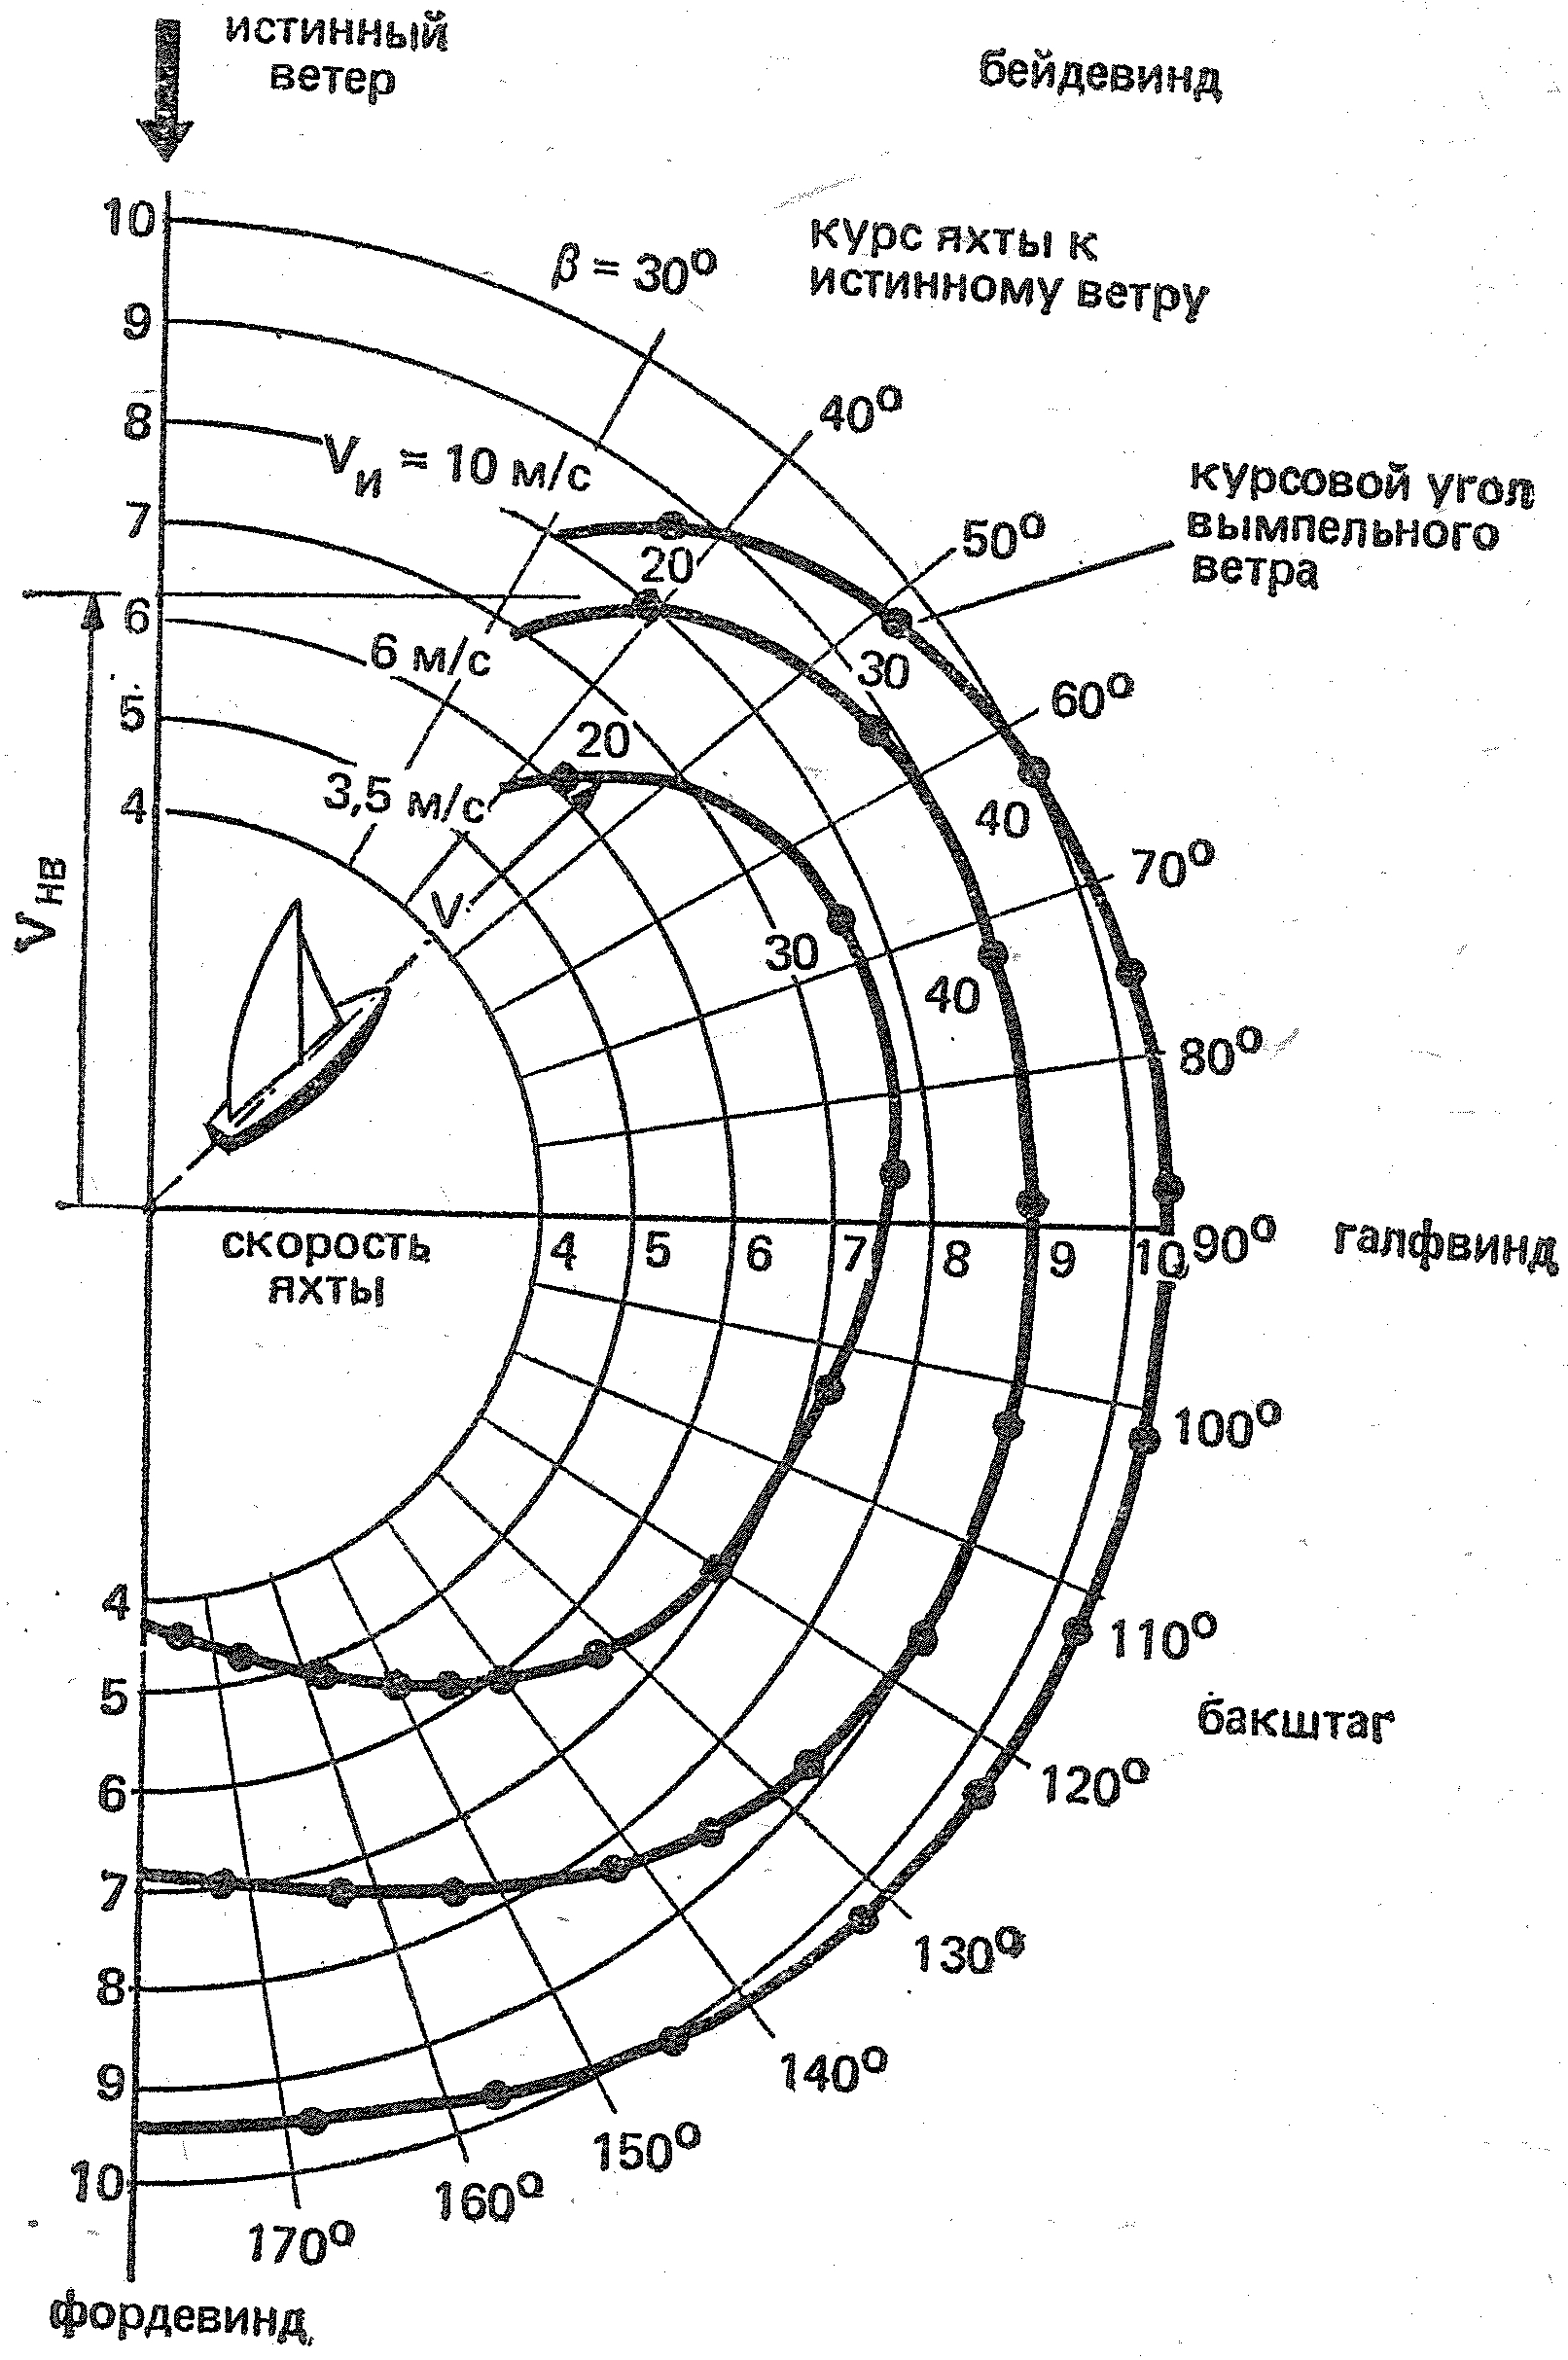
\includegraphics[scale=1.2]{0031P}
  \caption{Полярная диаграмма скорости яхты}
  \label{fig:31}
\end{figure}

Появившиеся в оснащении яхт приборы позволяют измерять параметры их движения и на основе этих измерений оценивать ходовые качества судна на разных курсах по отношению к ветру количественно, а не <<на глазок>>. Наиболее доступные приборы дают следующую информацию:

\begin{itemize}
\item угол между \textit{ДП} яхты и направлением вымпельного ветра; 
\item скорость вымпельного ветра; 
\item скорость яхты относительно воды; 
\item мгновенное изменение скорости яхты относительно выбранной точки отсчета. 
\end{itemize}

Пользуясь показаниями этих приборов, экипаж может оптимальным образом настроить паруса для каждого курса, чтобы получить наивысшую скорость, а также построить полярную диаграмму ходкости яхты (рис.~\ris{31}). При построении диаграммы яхта считается расположенной в центре нескольких концентрических окружностей, каждая из которых соответствует определенной скорости (4, 5, 6 и т.\=,д. уз). Из центра через 10\gr проводятся лучи, обозначающие курсы яхты по отношению к направлению истинного (или вымпельного) ветра. Для удобства в правой части диаграммы могут быть нанесены курсы судна относительно направления истинного, а по левую \--- относительно вымпельного ветра. Затем на каждом луче откладывается значение оптимальной скорости на данном курсе и при данной силе ветра.

Нетрудно заметить, что поляра скорости яхты на курсе от полного бейдевинда до крутого бакштага близка к дуге окружности, иными словами, с изменением курсового угла ветра скорость меняется очень незначительно. При переходе яхты на чистый фордевинд скорость заметно падает, особенно в слабый ветер. Объясняется это существенным снижением скорости вымпельного ветра и, поскольку аэродинамические силы пропорциональны ее квадрату, уменьшением силы тяги.

Постановка дополнительных парусов \--- спинакера и блупера помогает увеличить скорость яхты в слабый и средний ветер. В сильный же ветер, когда скорость оказывается близкой к предельной, $v = 3 \cdot {\lkvl}^{1/2}$, уз. и кривая сопротивления воды круто поднимается вверх, увеличение силы тяги при увеличении парусности практически не дает повышения скорости. На курсе бейдевинд скорость вымпельного ветра и аэродинамические силы максимальные, однако подъемная сила дает очень небольшую составляющую в направлении движения яхт (см. рис.~\ris{20}). С увеличением же на этом курсе крена уменьшается эффективный угол атаки относительно вымпельного ветра, падает величина аэродинамической силы и силы тяги. По этому на острых курсах более остойчивая яхта может оказаться быстроходней. 

С помощью полярной диаграммы рулевой яхты может решать различные тактические задачи, например выбрать оптимальный курс в лавировку. Он определяется по наибольшей скорости продвижения прямо против ветрa. Для этого следует провести касательную к поляре для данной силы ветра \--- перпендикуляр к его направлению. Точка касания поляры указывает наиболее выгодный курс. При плавании полным курсом, зная расстояние до конечной точки, можно с помощью поляры определить, как выгоднее будет пройти дистанцию \--- курсом фордевинд или двумя бакштагами со сменой галса.

Для того чтобы облегчить возможность использования полярной диаграммы, на кривых скорости наносят курсы яхты относительно вымпельного ветра. Получаются они построением треугольника скоростей по данным снятым с диаграммы (см. рис.~\ris{19}, \textit{б}) поскольку с движущейся яхты определить направление истинного ветра можно только приближенно \--- с помощью компаса и волны либо по береговым приметам.

\chapter{Некоторые особенности конструкции крейсерско-гоночных яхт}

\section{Классификация и основные требования, предъявляемые к крейсерско-гоночным яхтам}

Яхты для дальних плаваний (крейсерские яхты) можно разделить на три основные группы, отличающиеся по своему назначению: крейсерско\-/гоночные, крейсерские и туристские. 
Основным назначением \textbf{крейсерско\-/гоночных} яхт (их правильнее было бы называть гоночными яхтами открытого моря) является успешное выступление в маршрутных гонках на длинные дистанции. Крейсерско\-/гоночные яхты имеют характерное парусное вооружение с узкими и высокими парусами, свободную палубу, насыщенную механизмами и устройствами для управления парусами и их настройки (рис.~\ris{32}). Типичными представителями этой группы яхт являются, например, однотонник <<Марина>>, яхты <<Конрад-44>> и <<Конрад-54>>.

\begin{figure*}[htb]
  \centering
  \includegraphics[scale=1.3]{0032P}
  \caption{Однотонник <<Марина>> постройки ленинградской судоверфи ВЦСПС}
  \label{fig:32}
  \small
  \centering{}
  1 \--- гребной винт регулируемого шага; 2 \--- перо руля; 3 \--- скоб\-/трап; 4 \--- надувной спасательный плот ПСН-6М; 5 \--- привод натяжного ахтерштага; 6 \--- штурвал; 7 \--- путевой компас; 8 \--- приборная панель; 9 \--- главный компас; 10 \--- двухскоростная лебедка; 11 \--- односкоростная лебедка; 12 \--- входной люк; 13 \--- натяжка внутреннего штага; 14 \--- вант\-/путенс; 15 \--- фаловая лебедка; 16 \--- спинакер\-/гик; 17 \--- натяжка багштага; 18 \--- вентиляционный дефлектор
\end{figure*}

\textbf{Крейсерские яхты} \--- достаточно быстроходные суда, используемые для дальних спортивных плаваний определенной категории сложности и протяженности. Суда этого типа принимают также участие в морских гонках, хотя и с меньшими шансами на успех при выступлении в одной зачетной группе с гоночными яхтами. Крейсерские яхты, рассчитанные на многодневное пребывание экипажа на борту, имеют лучшие условия обитаемости, большие запасы пресной воды и топлива, часто снабжаются более мощным двигателем. Такие суда имеют палубные рубки, позволяющие увеличить объем внутренних помещений и их высоту; конструкцию корпуса, отвечающую правилам постройки классификационных обществ. При больших измерениях они оснащаются двухмачтовым вооружением. К судам этой группы можно, например, отнести однотонник, построенный небольшой серией на таллинской экспериментальной верфи спортивного судостроения, яхты типа <<Конрад-45>> и <<Опал>>.

\textbf{Туристские яхты} \--- мореходные и комфортабельные суда, рассчитанные на длительное плавание, не лимитируемое нормативами времени. Они оснащаются низким парусным вооружением с относительно небольшой площадью парусности, часто стилизуются под старинные кечи, шхуны и тендера. Мощный двигатель и топливные цистерны большой емкости позволяют получить высокую скорость и значительную дальность плавания под двигателем. По скорости и лавировочным качествам они уступают крейсерским. 

В зависимости от мощности двигателя, установленного на яхте, ее можно классифицировать как яхту парусно\-/моторную \--- со вспомогательным двигателем или как моторно\-/парусную. В первом случае мощность двигателя составляет 1,5\otdo 2,5~л.с. на каждую тонну полного водоизмещения яхты, что обеспечивает достижение скорости от 5 до 6 уз. По запасу топлива для двигателя яхта имеет дальность плавания 80\otdo 120 миль; используются гребные винты со складывающимися лопастями или флюгерного типа, оказывающие минимальное сопротивление движению яхты под парусами. Двигатель служит лишь для выхода из гавани и входа в нее, для коротких переходов в штилевых условиях и в аварийных ситуациях, а также для подзарядки аккумуляторных батарей. 

На моторно\-/парусных яхтах удельная мощность двигателя достигает 5\otdo 8~л.с./т.; запасы топлива для него принимаются из расчета обеспечения дальности плавания в несколько сотен миль со скоростью 8\otdo 10~уз. Устанавливаются эффективные трехлопастные гребные винты большого диаметра, оказывающие на ходу под парусами большое сопротивление движению. Наличие тяжелого двигателя и запасов топлива обусловливает уменьшение массы балласта до 15\otdo 25\,\% водоизмещения яхты, что, в свою очередь, заставляет ограничивать площадь парусности. Моторные парусники \--- это туристские яхты, у которых двигатель является таким же, если не более важным средством движения, как и паруса. 

По району плавания крейсерские яхты делятся на яхты для внутренних вод, озерного и прибрежного морского плавания и яхты для открытого моря (океанские). 

Для плавания по относительно закрытым внутренним водам, характерным невысокой волной и наличием большого числа пунктов, в которых яхта может укрыться от непогоды, мореходность яхт может быть ограничена, корпус, рангоут и такелаж могут иметь легкую конструкцию. Оптимальными типами судов для плавания по внутренним водам являются крейсерские швертботы, компромиссы, яхты с тяжелым подъемным килем и небольшие килевые суда, осадка которых не превышает 1,4~м. Поскольку при дальних спортивных плаваниях и гонках такие суда выходят в довольно обширные водохранилища с неприятной крутой волной, яхты для внутренних вод следует снабжать самоотливными кокпитами, предусматривать надежные закрытия входных и светлых люков и обеспечивать положительную остойчивость при крене до 90\gr \--- возможность самовыпрямления в аварийных ситуациях. 

Яхты, предназначенные для прибрежного морского и озерного плавания, должны быть рассчитаны на достаточно длительное противодействие сильному ветру и крупной волне и способность отлавировать от подветренного берега. Для таких судов обязателен самоотливной кокпит, прочный рангоут и такелаж, каюта достаточного объема, оборудованная койками для отдыха экипажа, работоспособный на волне камбуз, штурманский стол для ведения прокладки и компас. 

Наиболее жесткие требования к мореходности, оборудованию и снабжению предъявляются к яхтам открытого моря. 

Для судов, участвующих в гонках, эти требования дифференцируются в зависимости от сложности маршрута \--- категории гонок. 

Самые крупные и мореходные яхты, называемые неофициально яхтами нулевого класса, или макси\-/яхтами, имеют гоночный балл по правилам IOR, близкий к максимально допустимому значению 19\otdo 22~м. Такие суда строятся почти исключительно для трансокеанских и кругосветных гонок. Они рассчитываются на достижение максимально возможных скоростей на трассах с попутными ветрами с тем, чтобы ликвидировать преимущество, которое дает гандикап меньшим по размерам яхтам. Наибольшая длина макси\-/яхт составляет 21\otdo 24~м; длина по КВЛ \--- около 19~м; ширина \--- около 5,5~м; водоизмещение \--- 30\otdo 35~т; масса балластного фальшкиля \--- 16\otdo 18~т; осадка \--- до 3,6~м; обмерная площадь парусности \--- около 240\msq. В гонках экипаж таких яхт состоит из 13\otdo 17 человек. Корпуса их строятся из алюминиевых сплавов, реже \--- из стеклопластика или деревянной конструкции. 

Наиболее многочисленную группу яхт на любых гонках составляют яхты длиной от 10 до 12,5 м (III\--II классов IOR). Среди них имеется немало сравнительно дешевых однотипных судов, построенных по одному проекту что позволяет в ряде случаев выделить их в отдельные стартовые группы и повысить интерес экипажей к соревнованиям.
Дальнейшим развитием типизации является введение так называемых <<тонных>> или <<уровневых>> классов яхт, которые строятся по специальным правилам. Основным признаком для деления на классы служит величина гоночного балла IOR. Таких классов шесть: <<двухтонники>> (с гоночным баллом не более 32 футов \--- 9,76~м); <<однотонники>> (27,5 фута \--- 8,38~м); <<3/4-тонники>> (24,5 фута \--- 7,47 м); <<полутонники>> (21,7 фута \--- 6,60~м); <<четвертьтонники>> (18,5 фута \--- 5,65~м) и <<минитонники>> (16,5 фута \--- 5,18 м). Для каждого из этих классов имеются специальные требования к планировке корпуса, оборудованию и т.\=,п. Это типичные гоночные яхты ограниченной обитаемости, хотя участвуют в гонках на дистанциях 150\otdo 400 миль. Они могут выступать и в соревнованиях с яхтами других типов с учетом гандикапа.

Основным требованием, предъявляемым к крейсерско\-/гоночным яхтам, является их высокая эффективность в гонках при высоких мореходных качествах. 

Высокий надводный борт, большая ширина корпуса и значительная масса балласта (40\otdo 50\,\%) позволяют обеспечить достаточную остойчивость яхты для несения эффективной парусности в сильный ветер. Единственно приемлемым типом вооружения для крейсерско\-/гоночных яхт малых и средних размеров является бермудский шлюп благодаря его высоким аэродинамическим качествам. Яхта оснащается большим числом вспомогательных парусов, средств для их настройки, позволяющих получить максимальную тягу при ветре любой силы и на любом курсе яхты по отношению к нему. Работу экипажа с парусами облегчают палубные шкотовые и фаловые лебедки, стопора, оттяжки и т.\=,п. 

Крейсерско\-/гоночную яхту стараются оборудовать электронными приборами, облегчающими навигацию и ведение гонки. В их комплект входят эхолоты, лаги, указатели скорости и направления вымпельного ветра, курса яхты относительно него, радиопеленгаторы. На крупных и дорогих яхтах за рубежом не редкость специальные системы радионавигации <<Декка>>, <<Лоран>> и <<Омега>> и даже аппаратура для определения места с помощью искусственных спутников Земли. Большинство яхт снабжаются двумя\-/тремя радиостанциями УКВ и KB диапазонов для связи с берегом и судейским судном при участии в гонке. 

\section{Общее расположение и конструкция корпуса}

Обитаемости крейсерско-гоночных яхт должно уделяться достаточно внимания.

\begin{figure*}[htb]
  \centering
  \includegraphics[scale=1.3]{0033P}
  \caption{Общее расположение однотонника <<Марина>>}
  \label{fig:33}
  \small
  \centering{}
  1 \--- спасательный плот; 2 \--- привод натяжки ахтерштага; 3 \--- кокпит рулевого; 4 \--- колонка штурвала; 5 \--- ахтерлюк; 6 \--- путевой компас; 7 \--- поручень\-/стойка компаса; 8 \--- штурманский стол; 9 \--- кокпит шкотовых; 10 \--- топливный бак; 11 \--- входной люк; 12 \--- стойка лебедок и стопоров; 13 \--- светлый люк; 14 \--- степс; 15 \--- форлюк; 16 \--- носовой релинг; 17 \--- натяжка штага; 18 \--- паруса; 19 \--- форпик; 20 \--- салон; 21 \--- двигатель; 22 \--- аккумуляторы; 23 \--- конки; 24 \--- моторное отделение; 25 \--- камбуз; 26 \--- шкафы; 27 \--- диван; 28 \--- цистерна питьевой воды; 29 \--- унитаз; 30 \--- стол; 31 \--- умывальник. 
\end{figure*}

Типичным для гоночных яхт является общая компоновка и планировка внутренних помещений на яхте типа <<Марина>> (см. рис.~\ris{32} и \ris{33}). Характерной является палуба, свободная от рубок и надстроек, что диктуется необходимостью обеспечить удобство работы экипажа с парусами, а также снизить воздушное сопротивление, что важно при лавировке против сильного ветра. Для того чтобы получить нужную высоту внутри каюты, корпус яхты выполнен с повышенным бортом и значительной поперечной погибью палубы.

Гладкопалубный тип утвердился на яхтах меньших размерений вплоть до <<минитонников>>. Однако в большинстве случаев для того чтобы выдержать регламентируемую правилами классов высоту помещения, у входа устанавливается небольшая рубка, совмещенная с входным люком. 

Функционально размещение экипажа в двух кокпитах \--- рулевого в кормовом у самого транца и шкотовых \--- в кокпите близ миделя. Располагаясь позади всего экипажа, рулевой контролирует его действия, имеет хороший обзор парусов, а шкотовые не создают ему помех. Дифферентовка яхты в меньшей степени зависит от числа людей в кокпите, так как он находится ближе к общему центру тяжести судна, чем при традиционном кормовом расположении.

Под палубой экипаж располагается, по существу, в одном большом помещении в средней части яхты. Поперечная переборка, установленная под мачтой, отделяет форпик, используемый в качестве парусной кладовой. Здесь же размещены унитаз с принудительной прокачкой и небольшая раковина. 

Кают\-/компания, она же и каюта для отдыха, оборудована мебелью облегченной конструкции и газовым камбузом. Здесь же, близ центра тяжести яхты, установлен вспомогательный дизель, благодаря чему существенно снизилось его влияние на период килевой качки и соответственно уменьшился прирост сопротивления при лавировке против волны.

В кормовой части судна, отделенная легкой полупереборкой, расположена штурманская каюта со спальными местами для капитана и старшего помощника. Для оперативной связи штурмана или вахтенного начальника, ведущего прокладку по карте, с рулевым предусмотрен открывающийся светлый люк у переднего комингса рулевого кокпита.

Несколько иные принципы планировки общего расположения 15,3\--метровой яхты, рассчитываемой на длительные гонки и плавания в океане. Обеспечению комфорта для экипажа в данном случае уделяется больше внимания. Легкими переборками внутренний объем яхты делится на семь отсеков, или кают. Фор\-- и ахтерпики используются в качестве шкиперских кладовых. Паруса хранятся в носовом кубрике и в тамбуре перед мачтой, куда они подаются с палубы через сдвижной люк. 

Полная вместимость яхты по числу спальных мест составляет 13 человек, но трубчатые койки в носовом кубрике и над парусным рундуком используются только на стоянке и в тихую погоду. Наиболее комфортабельное помещение \--- кормовая трехместная каюта (для владельца или капитана) расположено в непроходной части и через небольшой лючок сообщается с кокпитом рулевого.

Кают\-/компания, камбуз и штурманская рубка расположены вблизи центра тяжести яхты, где меньше ощущается килевая качка и удары волн. Здесь же установлен вспомогательный дизель, закрытый звукоизолирующим капотом, под пайолами расположены цистерны с запасами топлива и питьевой воды.

Двухместная каюта в носовой части яхты может быть использована для размещения вахтенных начальников или гостей. 

\begin{figure}[htb]
  \centering
  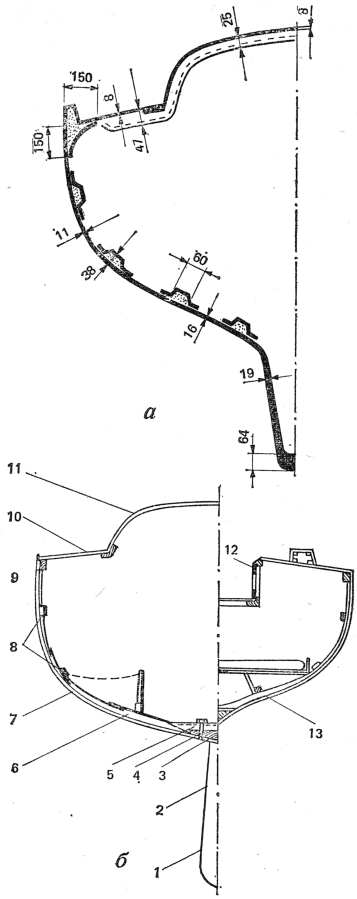
\includegraphics[scale=1.2]{0034P}
  \caption{Конструктивный мидель-шпангоут}
  \label{fig:34}
  \scriptsize
  \centering{}
а \--- пластмассовой яхты длиной 13,2 м; б \--- яхты деревянной конструкции длиной 12,8 м; 

1 \--- внутренний свинцовый балласт 2,73~т; 2 \--- плавник киля, сварной из стальных листов $\delta = 6$~мм; 3 \--- киль $90 \times 460$ мм; 4 \--- болт М25; 5 \--- флор, сталь $\delta = 6$~мм; 6 \--- ламинированный шпангоут $65 \times 125$~мм, клеенный из пяти реек по толщине; 7 \--- обшивка из семи слоев 3-миллиметрового шпона древесины каури (сорт красного дерева); 8 \--- стрингеры $25 \times 50$~мм; 9 \--- привальный брус $50 \times 75$~мм; 10 \--- палуба, три слоя фанеры толщиной по 6,4~мм; 11 \--- рубка, 7 слоев шпона каури $\delta = 3$~мм. 
\end{figure}

Объемы под койками, шкафы и закрытые полки используются для размещения личных вещей экипажа и запасов провизии в упаковке.

Освещение и вентиляция внутренних помещений осуществляется через входной люк и форлюк, снабженные прозрачными крышками, через открывающиеся светлые люки на палубе и иллюминаторы в комингсах рубки. В штормовую погоду помещения вентилируются через дефлекторные головки типа <<Дорадо>>.

Большую часть внутренних помещений яхты занимают койки, минимальная длина которых должна быть равна 1950~мм при ширине в голове 650 и в ногах 500~мм. Каждая койка снабжается закладной доской или парусиновым обвесом, предотвращающим падение людей при большом крене и качке.

Штурманский уголок оборудуется столом размером не менее $600 \times 1000$~мм для карт. Около стола или под ним размещаются ящики для карт, навигационных пособий и прокладочного инструмента. На переборке закрепляются индикаторы основных навигационных приборов: лаг, эхолот, указатель курса яхты по отношению к вымпельному ветру, компас, радиопеленгатор, барометр, часы и т.\=,п. Здесь же может быть установлена и судовая рация.

Камбуз оборудуется газовой плитой в карданном подвесе, разделочным столом, мойкой для посуды, ящиками, для расходных запасов провизии, полками для посуды. Для безопасной работы кока кастрюли должны надежно фиксироваться на плите, в удобных местах устанавливают поручни и подножные упоры, предусматривается откидное сиденье. 

Стол в кают\-/компании предпочтителен качающейся конструкции с противовесами маятникового типа и ограждением для посуды. Стол на <<Своне-51>> снабжен в средней части глубокими гнездами для удержания чашек с бульоном или кофе в штормовых условиях.

Подобная планировка типична для яхт длиной до 18~м и может быть названа сквозной или проходной, так как все помещения сообщаются между собой через вырезы в легких и прочных поперечных переборках. На более крупных яхтах применяется отсечный принцип планировки, при которой некоторые помещения (машинное отделение, форт- и ахтерпики) отделяются от остальных глухими водонепроницаемыми переборками и имеют самостоятельное сообщение с верхней палубой. 

От конструкции корпуса требуется не только высокая прочность, но и способность сохранять водонепроницаемость при длительных и многократно повторяющихся нагрузках.

Корпуса современных яхт строят из качественной древесины, стеклопластика и легких алюминиевых сплавов (реже \--- из стали и армоцемента). Стеклопластик в настоящее время наиболее распространенный в мире материал для постройки яхт, особенно малых и средних (до 16~м длиной) размеров. Благодаря применению методов холодного формования корпусов в специальных формах \--- матрицах из стеклопластика возможно изготовить корпус практически с любыми обводами. В отличие от деревянных и металлических яхт, корпуса которых собирают из множества деталей набора, обшивки и палубы, корпус пластмассовой яхты состоит из двух монолитных частей \--- собственно корпуса и палубы, которая формуется за одно целое с кокпитом и рубкой.

Прочной основой стеклопластика являются несколько слоев стекловолокнистых материалов. Синтетические смолы, которыми пропитываются стекломатериалы (на полиэфирной или эпоксидной основе), при затвердевании связывают слои прочной основы между собой и придают пластику водонепроницаемость. В наружный отделочный слой смолы вводится краситель-пигмент, так что при хорошем качестве изготовления пластмассовый корпус не нуждается в окраске (подводная часть пластмассовых яхт окрашивается необрастающими красками). В местах, требующих усиления, при формовании корпуса укладываются дополнительные слои стекломатериала или заформовываются конструкции из металла. 

Жесткость и прочность корпуса малых пластмассовых яхт обеспечивается переборками, деталями обстройки каюты, которые приформовываются к обшивке с помощью <<мокрых угольников>> \--- полос стеклоткани, пропитанных связующим. Толщина обшивки таких корпусов составляет от 5 до 15~мм. На яхтах длиной более 10~м обшивку дополнительно подкрепляют продольными стрингерами, выклеиваемыми заодно с обшивкой, или шпангоутами. Специальные подкрепления в виде флоров и продольных балок, разносящих нагрузку на большую площадь обшивки, приформовываются в местах приложения сосредоточенных нагрузок \--- у степса мачты, в районе крепления балластного фальшкиля, под двигателем (рис.~\ris{34}, \textit{а}).

Высокая прочность стеклопластика позволяет получить конструкцию необходимой прочности при малой толщине материала. Однако такая конструкция, например палуба, не обладает еще одним важным свойством \--- жесткостью, начинает <<дышать>> под нагрузкой. Для повышения жесткости палуб, переборок и наружной обшивки часто используют трехслойные (сэндвичевые) конструкции. Состоит такая конструкция из наружных тонких слоев стеклопластика и склеенного с ними внутреннего слоя \--- заполнителя из прочного легкого пенопласта или древесины бальзы. 

Кили на пластмассовых яхтах чаще всего делают в виде сварных профилированных коробок из нержавеющей стали, которые присоединяют к корпусу на сквозных болтах, проходящих через усиленные флоры. Иногда балласт в виде свинцовой или чугунной дроби укладывают в полость киля, отформованного совместно с корпусом, и заливают связующим, которое после отвердевания превращается вместе с дробью в монолит.

Корпуса пластмассовых яхт долговечны, легки, стойки к воздействию атмосферы и морской воды, не подвержены гниению и повреждению червями. Недостатком материала является чувствительность к истиранию и к действию концентрированных нагрузок.

Малая жесткость корпусов требует подкреплять их продольными переборками, как это, например, сделано на яхте <<Конрад-54>>, или трубчатыми ферменными конструкциями для предотвращения общего изгиба корпуса под действием тяги штагов и давления мачты.

В последние годы судостроительная древесина становится все более дефицитным и дорогим материалом на мировом рынке. Для яхтостроения применяются отборная высококачественная древесина тика, красного дерева и сибирского кедра (для обшивки) и дуба (для прочных деталей набора и вообще для всех частей судна), белого и гондурасского кедра. Используются также хорошо выдержанные прямослойная сосна и ель, а также лиственница.

В известной степени выручает широкое применение клееных конструкций и деталей, в которых можно использовать короткомерный материал. Благодаря качественному подбору древесины в клееной детали она оказывается более прочной при меньшем сечении. В целом корпус получается более легким и прочным, чем собранный на металлическом крепеже.

Клееной по пазам из реек выполняют и традиционную обшивку вгладь, которая ранее набиралась из досок и конопатилась. Клееная обшивка монолитная и водонепроницаемая, но имеет; недостаток \--- при сильных колебаниях влажности рейки могут трескаться и усыхать каждая в отдельности. Поэтому для стран с жарким климатом этот метод не применяется. Лучшие яхты строятся с обшивкой из тика в подводной части корпуса и из красного дерева в надводной.

Более легкая и прочная \--- двухслойная (а на самых крупных яхтах \--- и трехслойная) обшивка. Доски внутреннего слоя располагаются диагонально по отношению к ДП, а наружного \--- вдоль судна, поэтому такую обшивку часто называют диагонально\-/продольной. По правилам постройки яхт допускается уменьшение суммарной толщины двухслойной обшивки на 10\,\%, а трехслойной \--- на 15\,\% по сравнению с монолитной. 

С конца 60-х~гг. получил развитие еще один метод постройки деревянных корпусов яхт, при котором используются широкие полосы тонкого 3--4\-/миллиметрового шпона, укладываемые диагонально на позитивную форму \--- пуансон в несколько слоев (шпон для постройки легких гоночных швертботов и яхт применяется в зарубежной и отечественной практике еще с 30-х годов). Каждая полоса предварительно пропитывается разжиженным эпоксидным связующим, которое проникает глубоко в поры древесины и консервирует ее от загнивания, предотвращает проникновение в обшивку древоточцев. Поверх уложенного и закрепленного временно на пуансоне первого слоя наносится связующее и накладывается второй слой полос и т.д. Эпоксидная смола плотно заполняет все зазоры между кромками полос шпона и объединяет его слои в обшивку-скорлупу, подобную стеклопластиковой. Снаружи корпус может быть покрыт лаком или краской либо оклеен слоем стеклоткани. 

Корпуса небольших яхт по этому методу могут иметь безнаборную скорлупную конструкцию \--- прочность придают детали обстройки интерьера \--- переборки, рундуки и т.\=,п. Более крупные корпуса (самой большой построенной яхтой является 28-метровая копия старинного кэча) формуют прямо по набору, состоящему из редко расставленных переборок и рамных шпангоутов, а также из продольных реечных стрингеров, установленных через 160\otdo 200~мм. По этому же методу делают палубы с надстройками и рубки.

При постройке деревянных корпусов утвердилась поперечная система набора \--- с довольно часто расставленными шпангоутами. Правила постройки яхт регламентируют размеры связей корпуса для различных типов шпангоутов, но наибольшее распространение получила постройка корпуса на гнутых шпангоутах, на ламинированных из реек и на комбинации ламинированных и гнутых. Между парой ламинированных шпангоутов могут устанавливаться два или три гнутых. Для восприятия усилий от фальшкиля и давления мачты в корпусе устанавливают переборки, усиленные рамные шпангоуты (иногда выполняемые из металлических профилей). Внизу ветви шпангоутов соединяют деревянными листовыми или коваными металлическими флорами, разносящими нагрузку на достаточно большую часть шпангоута по ширине корпуса (рис.\ris{34}, \textit{б}).

Палубный настил на деревянных и металлических яхтах делается чаще всего из водостойкой фанеры. Фанерная палуба легче и прочнее обычного настила из палубника \--- не течет, не рассыхается под воздействием солнца, не требует постоянного ухода. Ее можно окрасить, оклеить стеклотканью на эпоксидном связующем или покрыть парусиной на краске. На фанеру могут быть наклеены тонкие декоративные планки из тика, имитирующие традиционный палубный настил. Нелакированная тиковая палуба обладает помимо прочих еще одним достоинством \--- по ней не так скользко ходить, как по палубе из другой древесины или окрашенной.
 
Корпуса многих крейсерско\-/гоночных яхт, особенно длиной более 15~м, построены цельносварными из алюминиево-магниевых сплавов. Сплавы эти (например, АМг5В) обладают высокой стойкостью против коррозии в морской воде, легко деформируются в холодном состоянии, хорошо свариваются в среде инертного газа аргона. Толщина наружной обшивки на яхтах длиной 15\otdo 16~м составляет 5\otdo 6~мм; килевой пояс может быть изготовлен из листов толщиной до 8~мм. За редким исключением, на алюминиевых яхтах используется поперечная система набора, причем расстояние между шпангоутами составляет 350\otdo 550~мм. Шпангоуты изготовляют из полособульбовых или тавровых прессованных профилей. Свинцовый или чугунный фальшкиль должен быть надежно изолирован от алюминиевого корпуса с помощью битумной мастики или эпоксидного компаунда.

Крейсерско\-/гоночные яхты из стали в последние годы строят крайне редко, хотя в конце 60-х~гг., когда стальной корпус давал яхте преимущество при обмере по правилам RORC, было построено немало стальных <<однотонников>> и даже яхт меньших размерений. Толщина наружной обшивки на цельносварных яхтах длиной 12\otdo 18~м варьируется от 4 до 6~мм.

Так как сталь и алюминий обладают лучшей теплопроводностью, чем дерево и стеклопластик, на яхтах из этих материалов необходима тепловая изоляция жилых помещений. Такая изоляция в виде плит из экспанзита (прессованная пробка), поропласта и других материалов наклеивается изнутри на наружную обшивку и зашивается декоративными материалами \--- пластиком, фанерой, линкрустом.

Палубы и надстройки металлических яхт изготавливают из фанеры или металла с покрытием деревянным настилом или нескользящей мастикой. 

\section{Устройства, системы и снабжение крейсерско-гоночных яхт}

Безопасность эксплуатации и обитаемость яхты в большой степени зависят от того, насколько хорошо судно оснащено соответствующим оборудованием, устройствами и системами. К числу важнейших судовых устройств относятся якорно\-/швартовное, рулевое, леерное устройства и яхтенный тузик.

\textbf{Якорное устройство.} Количество и вес становых якорей, калибр якорной цепи и ее длина для крейсерских яхт определяются правилами классификации и постройки (табл.~\ref{tab:2}). Яхта, уходящая в дальнее плавание, должна быть укомплектована не менее чем двумя становыми якорями, один из которых примерно на 20-25\,\% должен быть тяжелее основного, наиболее часто используемого якоря. Кроме того, на судне должны быть завозные якоря или верпы. Масса самого большого верпа (cтоп\-/анкера) принимается обычно равной 75\,\% основного станового якоря, а самого легкого \--- дрека \--- 25\,\% станового.
Наиболее распространенным типом якоря на отечественных яхтах остается адмиралтейский якорь, обладающий высокой держащей силой практически на любом грунте. К недостаткам адмиралтейского якоря относят сравнительно большую массу и необходимость вооружать его перед каждой постановкой на якорь. 

\begin{table*}[htb]
  \centering{}
  \begin{tabular}{p{0.4\textwidth}|c|c|c|c}
    \toprule
    Классы яхты IOR & VI & V & IV~--~II & III \\
    \midrule
    \textbf{Якоря:} \\ 
    количество, шт. &  1 & 1 & 2 & 2 \\
    вес, кг & 15 & 18 & 12, 18 & 18, 25 \\ 
    \midrule
    \textbf{Якорная цепь:} \\
    длина, м & 30 & 30 & 40 & 60 \\
    калибр, мм & 5 & 6 & 7 & 8 \\
    \midrule
    \textbf{Якорный канат:} \\
    окружность, мм & 30 & 50 & 60 \\
    длина, м & 55 & 60 & 70 \\
    \midrule
    \textbf{Завозной канат:} \\
    окружность, мм & 40 & 50 & 60 & 60 \\
    длина, м & 45 & 50 & 55 & 60 \\
    \midrule
    \textbf{Швартовые концы:} \\
    окружность, мм & 45 & 50 & 55 & 60 \\
    длина, м & 5 & 5 & 6 & 8 \\
    \midrule
    \textbf{Ведра}, шт. & 1 & 1 & 1 & 2 \\
    \midrule
    \textbf{Помпа водоотливная} 
    с диаметром цилиндра не менее, мм & 25 & 30 & 40 & 50 \\
    \bottomrule
  \end{tabular}
  \caption{Нормы снабжения крейсерско\-/гоночных яхт якорями, якорными и швартовыми канатами и водоотливными средствами}
  \label{tab:2}
  \textbf{Примечание. }Вес якорей указан для адмиралтейского якоря. При применении бесштоковых якорей их вес должен быть на 25\,\% больше. В случае применения якорей повышенной держащей силы они подбираются по величине держащей силы, которая должна быть не менее, чем у адмиралтейского якоря, указанного в таблице.
\end{table*}

На яхтах находят применение также легкие бесштоковые якоря с поворотными лапами типа Данфорта, Матросова и Холла, а также якорь\-/плуг (или лемеховый). Относительно своей массы якоря Данфорта, Матросова и лемеховый развивают очень высокую держащую силу на песчаных грунтах и в плотном иле, но уступают адмиралтейскому при стоянке на каменистом грунте и гальке. Кроме того, при съемке в сильный ветер, когда яхту без помощи двигателя трудно привести в положение <<панер>>, требуются большие усилия для отрыва якорей этих типов от грунта. 

Для определения необходимой массы адмиралтейского якоря можно воспользоваться приближенной формулой:

\begin{equation}
  W = 8 \sqrt[3]{D^2}, \quad \text{кг}
\end{equation}

где $D$ \--- водоизмещение яхты в тоннах. Массу второго якоря можно принять равной 75\,\% массы первого. Калибр якорной цепи подсчитывается по формуле: 

\begin{equation}
  d = 4,7 \sqrt[3]{D}, \quad \text{мм}
\end{equation}

Якорные цепи предпочтительнее канатов, так как цепь благодаря большой массе прижимает веретено якоря к грунту и амортизирует рывки яхты при волнении. 

При стоянке на якоре цепь или канат крепятся на яхте за прочный битенг, кнехт или берется на стопора. Специальные механизмы для выборки каната или цепи \--- шпили и брашпили применяются только на самых крупных яхтах длиной свыше 15~м. Для отрыва якоря от грунта на яхтах меньших размерений применяют тали со скобой, перекладываемой за звенья цепи.

Чем ближе к форштевню закреплены клюзы, полуклюзы или роульс для якорной цепи, тем меньше яхту водит на стоянке и легче выбирается цепь. Лучшим устройством считается роульс со стопором, установленный на форштевне.

Для размещения якорных цепей яхты оборудуются цепными ящиками. Предпочтительнее узкие и высокие ящики, в которые цепь <<самоукладывается>> без завалов и калышек. Конец цепи крепится на судне к жвака\-/галсу \--- короткому куску цепи с быстроотдающимся устройством, которое при полном вытравливании якорь\-/цепи появляется из палубного клюза и готово к немедленной отдаче. 

Необходимым дополнением якорного устройства являются томбуй и буйреп, а также крепления якорей по\-/походному на их штатных местах. 

\textbf{Швартовное устройство} состоит из битенгов и кнехтов, установленных в носовой и кормовой частях палубы, киповых планок (полуклюзов), придающих швартовам правильное направление и предохраняющих их от перетирания о ватервейс или фальшборт. Длину швартовных концов, для которых используются синтетические тросы из капрона, лавсана и т.\=,п., рекомендуется принимать равной удвоенной длине яхты, а диаметр подбирать так, чтобы разрывная нагрузка троса была бы не меньше водоизмещения яхты. 

\begin{figure}
  \centering
  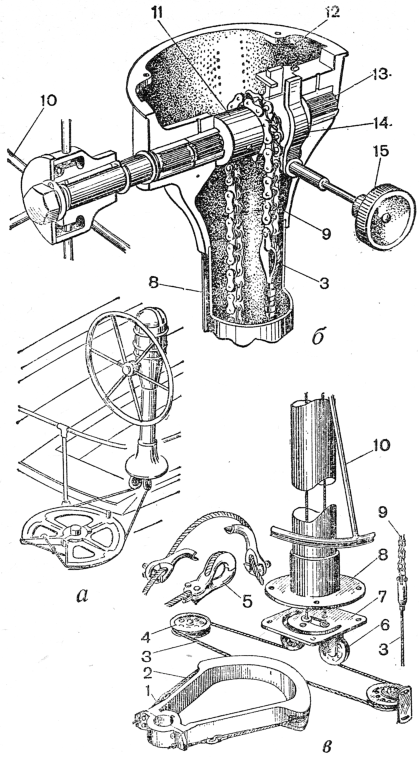
\includegraphics[scale=1.2]{0035P}
  \caption{Рулевой штуртросовый привод со штурвальной колонкой}
  \label{fig:35}
  \small
  \centering{}
  1 \--- натяжное устройство; 2 \--- сектор; 3 \--- штуртрос; 4 \--- направляющий шкив; 5 \--- разъемный коуш; 6 \--- самоустанавливающийся блок; 7 \--- плита блоков; 8 \--- колонка; 9 \--- цепь Галля; 10 \--- штурвал; 11 \--- звездочка; 12 \--- корпус рулевой машинки; 13 \--- игольчатый подшипник; 14 \--- колодочный стопор; 15 \--- привод стопора.
\smallskip
\end{figure}

\textbf{Рулевое устройство.} Румпель \--- наиболее простое и надежное устройство, при котором рулевой хорошо чувствует яхту, если, конечно, рулевые петли хорошо отцентрированы и правильно выбран коэффициент компенсации балансирного руля. Недостатком румпеля являются его длина, мешающая работе в кокпите, и довольно значительные усилия при управлении яхтой в свежий ветер. В большую волну при попутных ветрах иногда приходится управлять яхтой с помощью румпель\-/талей, между румпелем и подходящими утками на палубе. 

Яхты свыше 10~м длиной иногда управляются с помощью штурвала большого диаметра и тросовой передачи на сектор, закрепленный на баллере над сальником гельмпорта (рис.~\ris{35}).

Штурвал устанавливается в кокпите на рулевой колонке (\textit{а}) и имеет на валу звездочку (\textit{б}), которую огибает роликовая цепь, включенная в среднюю часть штуртроса. Если на колонке стоит компас, то детали привода и цепь делаются из немагнитных материалов. Для передачи применяется гибкий стальной трос конструкции $6 \times 19 +$ос достаточного диаметра, чтобы выдержать рывки, передаваемые рулем на волнении. Критическое значение имеют диаметры направляющих шкивов и их ориентация точно по оси троса; диаметр шкива по желобку для троса должен быть не менее 16\otdo 19 диаметров троса.

Штуртросовый привод не является самотормозящимся в отличие от ранее применявшихся винтовых рулевых машинок, поэтому рулевой сохраняет (при отсутствии люфтов) хорошее чувство руля. Тормоз, имеющийся на колонке, позволяет застопорить руль в определенном положении и на стоянке. Сектор (\textit{в}) (иногда он заменяется диском с желобками для троса) снабжается тросовыми или другими ограничителями поворота руля. 
 
\textbf{Леерное устройство} состоит из жестких трубчатых ограждений \--- релингов, установленных в носу и корме, стоек и лееров. Размеры и конструкция леерного ограждения регламентируются правилами обеспечения безопасности плавания при проведении крейсерских гонок.

Для того чтобы большой генуэзский и стаксель не ложился на леера, носовой релинг выполняют разрезной конструкции \--- со щелью, в которую проходит нижняя шкаторина генуи на острых курсах. На леерах в районе кокпита закрепляют парусиновые обвесы, защищающие экипаж от ветра и брызг. С внутренней стороны на них пришивают карманы для бросательного конца и других мелких предметов снабжения, которые желательно иметь на палубе.

На яхте, выходящей в крейсерское плавание, \textbf{тузик} является необходимой деталью снабжения. Минимальные размеры тузика, позволяющие безопасно использовать его на закрытых акваториях: длина \--- 2,4~м, ширина \--- 1,2~м, высота борта \--- 0,4~м. Предпочтительнее тузики с катамаранными обводами или с носовым транцем, как более вместительные и остойчивые на волнении. Существенными деталями оборудования тузика являются мягкий круговой кранец, закрепленный по привальному брусу, рым для буксировки в нижней части форштевня или на киле, гнездо в транце для голанения и подвески якоря при его завозе. На палубе яхты или на крыше рубки предусматривают подушки для укладки тузика и обушки для крепления найтовов. Для подъема шлюпки массой более 100~кг на палубу используются гик, специальная стрела или шлюпбалки. 

\textbf{Системы.} Крейсерско\-/гоночные яхты оборудуются осушительной, сточной, вентиляционной системами, а также системами водо- и газоснабжения. 

Осушительная система состоит из ручных насосов, приемных трубопроводов с сетками и отливных трубопроводов, выведенных за борт выше ватерлинии. Применяются ручные диафрагменные помпы, одно- и двухцилиндровые насосы, а также насосы-альвееры. Правила классификации оговаривают производительность насоса или Диаметр его цилиндра (см. табл.~\ref{tab:2}). Диаметр трубопроводов составляет обычно половину диаметра цилиндра. 

Согласно правилам безопасности крейсерских гонок, на яхтах, участвующих в гонках 1--3-й категорий, одна из помп обязательно должна быть установлена так, чтобы ею можно было пользоваться из кокпита, когда все входные люки закрыты. Простейший вариант \--- всасывающая поршневая помпа, смонтированная в днище кокпита, в который она подает трюмную воду, сливающуюся самотеком через отливные шпигаты. 

Если отливной трубопровод выводится за борт, он должен быть снабжен невозвратно\-/запорным клапаном.

К приемнику осушительного насоса должен быть обеспечен беспрепятственный сток воды через все флоры и переборки либо к распределительному коллектору у помпы из каждого отсека подводятся отдельные трубопроводы.

Система водоснабжения на яхте состоит из цистерн пресной воды (они обычно размещаются под пайолами вблизи центра тяжести яхты), наливных и воздушных труб, расходных трубопроводов с насосом и кранами.

Цистерны большой емкости снабжают продольными отбойными переборками. Наливная труба заканчивается на палубе герметичной резьбовой пробкой, а конец воздушной трубки располагается так, чтобы исключить попадание внутрь цистерны морской воды и быть на виду при заполнении цистерн.

На яхтах получили распространение две системы подачи воды из цистерн к раковинам на камбузе и в умывальнике: гравитационная \--- самотеком из небольшой расходной цистерны, располагаемой под палубой, или под давлением воздуха, которое создается при нагнетании воды в полузаполненную расходную цистерну (гидрофор) (рис.~\ris{36}). Гидрофор располагается под пайолами и не занимает полезного объема внутри яхты. В обоих случаях насос пресной воды может быть ручным или с электроприводом от аккумуляторной батареи. Вода на камбуз может подаваться с помощью ручной или педальной диафрагменной помпы непосредственно к расходному крану.

\begin{figure}[htb]
  \centering
  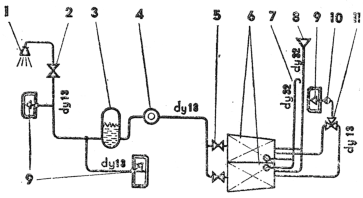
\includegraphics[scale=1.2]{0036P}
  \caption{Схема системы водоснабжения с гидрофором (под давлением)}
  \label{fig:36}
  \small
  \centering{}
  1 \--- душ; 2 \--- запорный кран \textit{dу} 13; 3 \--- гидрофор емкостью 30 литров; 4 \--- нагнетательный насос; 5 \--- запорный кран \textit{dy} 18; 6 \--- цистерны пресной воды; 7 \--- воздушная трубка; 8 \--- заливная горловина; 9 \--- раковина; 10 \--- педальная диафрагменная помпа; 11 \--- трехходовый кран \textit{dy} 13 (\textit{dy} \--- внутренний диаметр трубопровода)
\end{figure}

Постоянно повышающиеся требования к чистоте водной среды не оставляют в стороне и спортивные суда. В настоящее время на многих яхтах устанавливают специальную сточную систему, содержащую цистерну, в которой собираются загрязненные воды от камбуза, умывальника и гальюна. Опорожнение этой цистерны производится с помощью специальных установок в гаванях. Непосредственный выброс сточных вод за борт допускается во многих районах моря только за пределами трехмильной прибрежной зоны. 

Унитазы на яхтах, как правило, оказываются расположенными ниже ватерлинии, вследствие чего необходимо специальное устройство для промывки забортной водой и откачки грязной воды за борт, если судно не оборудовано сточной цистерной. 

На многих яхтах используются газовые камбузные плиты. При значительном числе экипажа и автономности плавания требуется установка баллонов большой емкости и монтаж системы газоснабжения. 

Пропан\-/бутан тяжелее воздуха, оказывает отравляющее действие на организм человека, и смесь его с воздухом в определенной пропорции взрывоопасна. Поэтому к системе газоснабжения предъявляются особые требования. Баллоны с газом должны устанавливаться в вертикальном положении, желательно в помещении, изолированном от жилых кают или на верхней палубе. Дно помещения для баллонов должно располагаться выше ватерлинии и иметь шпигат для стока газа за борт. Отсек баллонов должен хорошо вентилироваться. 

Газовые баллоны снабжаются редукционными клапанами для понижения давления с 8\otdo 16~атм до 0,05~атм. Трубопровод, соединяющий баллон с плитой, выполняется из медных труб или дюритового шланга с минимальным количеством соединений и с запорным краном перед плитой. 

\begin{figure}[htb]
  \centering
  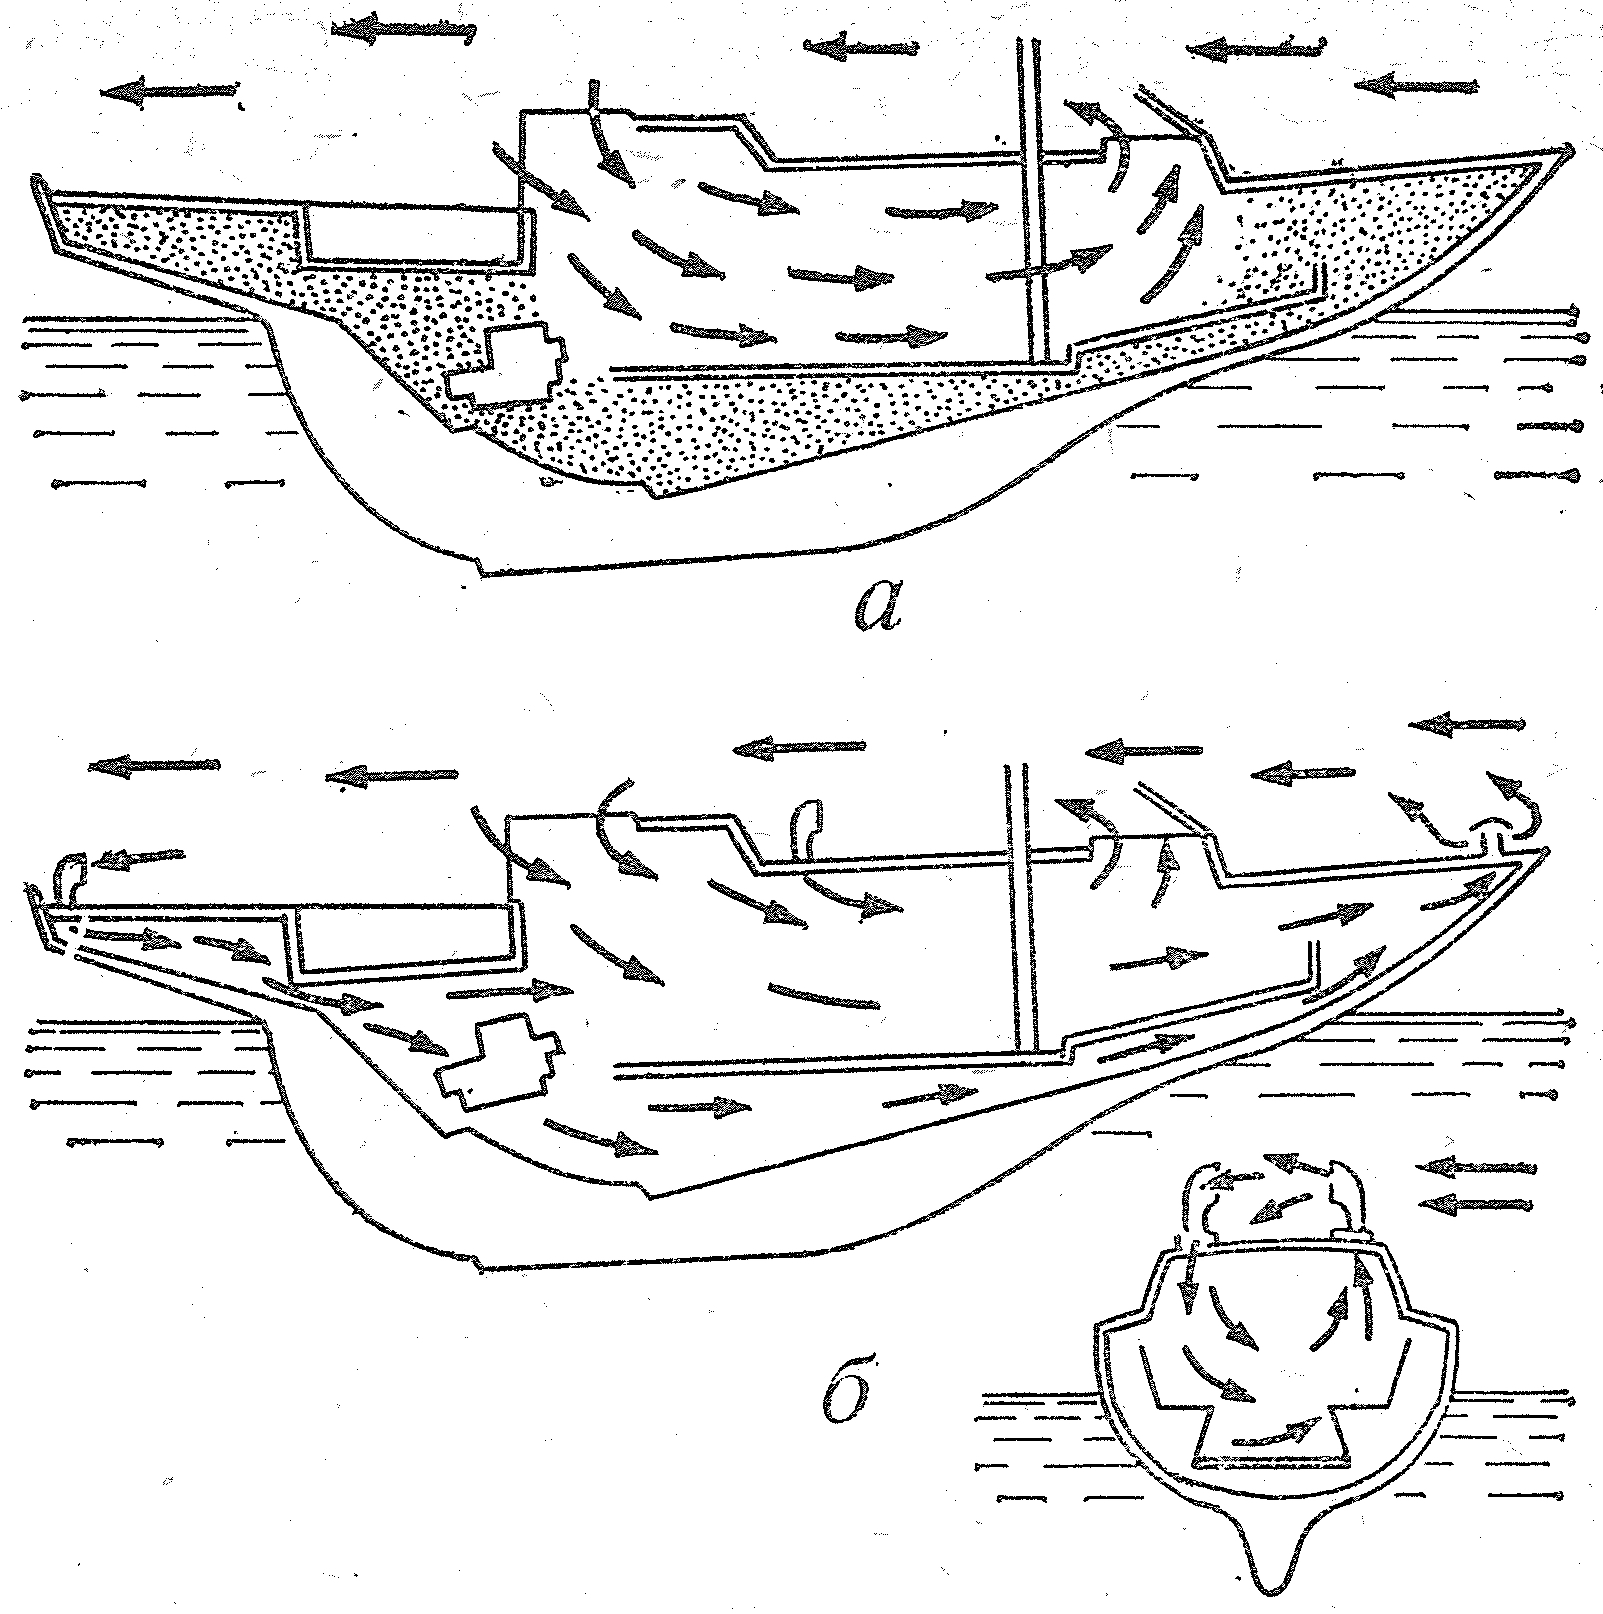
\includegraphics[scale=1.2]{0037P}
  \caption{Схема циркуляции воздуха в помещениях яхты}
  \label{fig:37}
  \small
  \centering{}
  \textit{а} \--- недостаточная циркуляция воздуха (заштрихованы невентилируемые объемы); \textit{б} \--- правильная циркуляцня воздуха
\end{figure}

Система естественной вентиляции должна обеспечивать непрерывную циркуляцию воздуха во всех помещениях яхты (рис.\ris{37}). Это возможно, если расположить нагнетательные вентиляционные головки в корме, а поток воздуха в помещениях судна направить с кормы в нос. Хорошая вентиляция важна не только для нормальных условий жизни экипажа в море, но и для увеличения срока службы самой яхты. При плохой вентиляции (особенно трюма и пространства между наружной и внутренней обшивками) на деревянных деталях корпуса появляется грибковая плесень и гниль. 

Наиболее распространенные тип вентиляционных головок, используемые как для притока, так и вытяжки представлены на рис.~\ris{38}. 

\begin{figure}[htb]
  \centering
  \includegraphics[scale=1.2]{0038P}
  \caption{Вентиляционные головки брызгозащищенного типа для яхт}
  \label{fig:38}
  \small
  \centering{}
  \textit{а} \--- типа <<Дорадо>>; \textit{б} \--- фирмы <<Никро Фико>>
\end{figure}

При установке вспомогательного двигателя моторный отсек отделяется от остального трюма водонепроницаемым флором или переборкой. Под двигатель устанавливают поддон для сбора утечек топлива и масла. Топливные баки располагают по возможности (бензобаки \--- обязательно) вне моторного отсека, а горловины для их заполнения и воздушные трубки выводят на палубу. 

Двигатели обслуживаются системами: топливной, водяного охлаждения, газовыхлопной. 

\textbf{Электрооборудование.} Для внутреннего освещения кают и питания навигационных огней применяется постоянный ток напряжением 6\otdo 12~в на малых яхтах и 24~в \--- на больших. Источниками тока служат кислотные или щелочные аккумуляторные батареи, которые подзаряжаются от генератора, навешенного на двигатель, или через зарядное устройство от береговой сети. Емкость батареи составляет обычно 100\otdo 300~а-ч. 

Мощность ламп для внутреннего освещения кают достаточна 15\otdo 25~вт, Для навигационных огней и освещения палубы \--- 12\otdo 15 вт. Отличительные бортовые огни устанавливают на носовом релинге, на комингсах рубки или на краспицах таким образом, чтобы их не закрывали паруса. Белый топовый огонь, который яхта должна нести при движении под мотором, устанавливается на передней мачте на высоте 2\otdo 5~м над палубой, а кормовой \--- на кормовом релинге или гакаборте\footnote{На яхте ё--- край палубы на корме у транца, ограниченный его шириной.}. В качестве якорного штагового огня можно использовать переносную лампу; для сигнализации служит клотиковый огонь, устанавливаемый на топе мачты. Яхты внутреннего плавания должны быть снабжены импульсными лампами\-/отмашками, расположенными на вантах или комингсах рубки. 

Для освещения палубы и парусов на нижних краспицах устанавливают фары мощностью 6\otdo 12~вт. Для освещения компаса, штурманского стола и камбуза предусматривается автономное освещение. 

Аккумуляторы устанавливают в моторном отделении вблизи стартера двигателя и заключают в водонепроницаемые ящики с вентиляционными трубками. Электропроводка выполняется морским кабелем. Потребители электроэнергии разбиваются на несколько групп, каждая из которых снабжается на распределительном щите отдельными предохранителями и выключателями. 

\section{Парусное вооружение}

Подавляющее большинство крейсерско\-/гоночных яхт, принимающих участие в гонках, оснащается одномачтовым вооружением типа шлюп даже при площади парусности 150\otdo 200\msq. Шлюп обладает высокими тяговыми характеристиками, прост в управлении и обеспечивает хорошую управляемость яхты. 

Однако при увеличении парусности свыше 100\msq становятся ощутимы недостатки оснастки этого типа, которые требуют подчас сложных конструктивных решений. Увеличивается высота мачты и соответственно размеры ее поперечного сечения и масса: для раскрепления мачты требуется тяжелый стоячий такелаж. Высокое расположение центра парусности вызывает необходимость повышать остойчивость, увеличивать массу балласта. При усилении ветра экипажу приходится брать рифы на гроте и заменять передние паруса на меньшие по площади. В прошлом при парусности 60\otdo 200\msq яхты нередко оснащались вооружением типа иол. Площадь бизани на иоле составляет всего 10\otdo 12\,\% общей площади парусности, и роль этого паруса в создании тяги невелика. Бизань, однако, оказывает существенное влияние на центровку яхты, обеспечивает исключительную поворотливость, особенно когда в штормовых условиях несут небольшой стаксель в комбинации с бизанью. 

Вооружение типа кэч, которое целесообразно при оснащении яхт парусностью 120\otdo 250\msq благодаря более равномерному распределению общей площади между тремя основными парусами (бизань \-- 20\otdo 25\,\%, грот \--- 45\otdo 50\,\%, стаксель \--- 30\otdo 35\,\%) предпочитается для оснащения крейсерских и гоночных океанских макси\-/яхт. Для уменьшения влияния стекающего с грота потока воздуха на работу бизани бизань\-/мачту часто относят на значительно большее расстояние от грот\-/мачты, чем при традиционной оснастке этого типа.

Кэч обладает заметно худшими качествами на лавировке, чем шлюп или иол, но лучше идет под стакселем и бизанью и устойчивее лежит в дрейфе, чем иол. 

Тендер в его классическом виде \--- с двумя или тремя передними парусами \--- стакселем и кливером, так же как и шхуна, в последние годы практически не применяется. Многие шлюпы снабжаются внутренним (нижним) штагом, на котором могут ставиться дополнительные стаксели как в слабые, так и в свежие ветра. Но основную роль играет топовый генуэзский стаксель. Шхуной вооружают яхты парусностью 200\otdo 300\msq, причем используется преимущественно стаксельное вооружение. 

В 60-е~гг. крейсерско\-/гоночные яхты предпочитали вооружать шлюпом с топовым стакселем, поскольку стаксель является более эффективным парусом, чем грот. К тому же при топовой оснастке допускается постановка спинакера большей площади, чем при оснастке типа 7/8 или 3/4 \--- по положению точки крепления основного штага относительно общей высоты мачты. В последние годы, однако, наметилась тенденция вновь оснащать яхты, особенно младших классов (четверть- и полутонники) шлюпом типа 7/8 или 3/4. Как показал опыт параллельных испытаний однотипных яхт, топовый и 7/8 варианты равноценны по лавировочным качествам. На полных курсах яхта с топовой оснасткой получает преимущество в скорости благодаря большей площади спинакера. Однако уже на крутом бакштаге из-за малой площади грота топовый шлюп проявляет склонность к брочингу. На бакштаге и галфвинде шлюп типа легче в управлении как благодаря меньшей величине сил, действующих на спинакере, так и за счет повышения роли грота.

К достоинствам оснастки типа 7/8 относят также меньшее сечение мачты и возможность регулировать ее изгиб с помощью штагов и бакштагов. Этот тип оснастки лучше для сильных и свежих ветров; топовая оснастка предпочтительна для слабого ветра.

Подавляющее большинство яхт оснащается мачтами, изготовленными методом прессования из алюминиево-магниевых сплавов. Оптимальные весовые характеристики получаются в случае использования профилей мачты с переменной толщиной стенки, утолщающейся в тех местах поперечного сечения, где действуют наибольшие напряжения (рис.~\ris{39}). Соотношение размеров продольной и поперечной оси сечения составляет 1,25\otdo 1,50. Для яхт меньших размерений применяются мачты овального сечения и с постоянной толщиной стенки. 

Деревянные мачты выполняются клееной пустотелой конструкции овального или прямоугольного сечения со скругленными углами. Толщина стенок составляет 1/5 поперечного размера, а в местах крепления такелажа и в нижней части мачта делается сплошной.

Алюминиевые мачты на 40\,\% легче деревянных и более надежны в длительной эксплуатации и позволяют сделать внутреннюю проводку фалов, чем существенно снизить воздушное сопротивление.

\begin{figure}[htb]
  \centering{}
  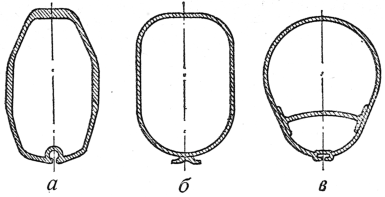
\includegraphics[scale=1.2]{0039P}
  \caption{Поперечное сечение мачт из легкого сплава}
  \label{fig:39}
  \centering{}
  \small
  \textit{а} \--- мачта с переменной толщиной стенки для топовой оснастки крупных яхт; \textit{б} \--- мачта крейсерской яхты водоизмещением около 3~т; \textit{в} \--- мачта мореходной крейсерско\-/гоночной яхты
\end{figure}

Стоячий такелаж изготавливается из жестких стальных тросов конструкции $1 \times 19$ \--- спиральной свивки из 19 нержавеющих стальных проволок. В отечественной практике применяется трос $6 \times 7 + $\,1ОС, а на зарубежных яхтах можно видеть такелаж из сплошной нержавеющей проволоки. Следует помнить, что от жесткости троса зависит распределение нагрузки от парусов между мачтой и стоячим такелажем. Чем меньше проволок в пряди при данном диаметре троса, тем больше его жесткость и тем на меньшую длину он растягивается при повышении нагрузки \--- усилении ветра. Особенно важно иметь жесткий трос на стоячем такелаже в верхней части мачты \--- на топ\-/вантах, штаге и ахтерштаге с тем, чтобы уменьшить его прогиб, который увеличивается по мере удаления от опорной точки \--- пяртнерса или степса. 

Суммарная разрывная нагрузка, которую должны выдерживать ванты одного борта, составляет около $1,25D$ \--- водоизмещения яхты. Это показатель не только прочности, но и жесткости стоячего такелажа. Между отдельными вантами суммарную нагрузку можно распределить в зависимости от схемы раскрепления мачты такелажем, и в первую очередь от количества краспиц (рис.~\ris{40}). 

Для штага и ахтерштага при топовом стакселе применяют такой же трос, как и для самых прочных вант. Следует учитывать, что обрыв штага равносилен потере мачты. При оснастке типа 7/8 штаг должен иметь такую же прочность, что и одиночные нижние ванты; ахтерштаг и бакштаги \--- не менее прочности троса для верхних вант. 

\begin{figure}[htb]
  \centering{}
  \includegraphics[scale=1.2]{0040P}
  \caption{Схема раскрепления мачт крейсерско-гоночных яхт и нагрузки на ванты в процентах от общего усилия}
  \label{fig:40}
\end{figure}

Важное значение имеет угол между мачтой и вантой. Угол менее 12\gr можно считать недостаточным \--- получается большое усилие сжатия в мачте, а ванты необходимо вырубать из более толстого троса. Оснастка с тремя парами краспиц позволяет увеличить угол между вантами и мачтой в полтора раза. Длина нижних краспиц при трех рядах краспиц может быть увеличена, так как ближе к палубе <<пузо>> генуи увеличивается и она не касается концов краспиц. 

Стоячий такелаж яхты является инструментом для настройки грота и оказывает влияние на работу стакселя. Если на малых яхтах (швертботах) в слабый ветер при прогибе топа мачты на подветренную сторону нагрузка на грот и крен яхты уменьшается, то на больших судах это недопустимо. Отклонившийся от среднего положения топ означает уменьшение угла между мачтой и вантой, снижение поддерживающей способности ванты, увеличение прогиба штага. Кроме того, увеличивается плечо приводящего к ветру момента. 

Поэтому на яхтах с топовым вооружением важно установить топ мачты жестко и точно в \textit{ДП} и не допускать его отклонения под нагрузкой. При установке мачты ее выравнивают с помощью клиньев в пяртнерсе строго по \textit{ДП}. Затем, подняв на грота\-/фале рулетку, регулируют положение топа с помощью натяжения верхних вант, контролируя по рулетке равные расстояния от топа до симметричных относительно \textit{ДП} точек на правом и левом фальшбортах. Затем добиваются с помощью натяжения средних и нижних вант прямолинейности ликпаза по всей высоте мачты. 

Верхние ванты набивают так, чтобы на ходу в средний ветер при крене 15\otdo 20\gr подветренная ванта была бы не слишком туго набита, не имела бы слабины. Натяжение средних и нижних вант делается несколько меньше. Если нижние ванты двойные, то сначала набивают передние, с тем чтобы они были несколько более тугими. 

Необходимое натяжение придается штагу обычно с помощью ахтерштага при топовом вооружении и бакштагов при оснастке типа 7/8. Ахтерштаг выбирается так туго, как только это возможно: предварительное его натяжение может составлять 30\otdo 40\,\% разрывной нагрузки троса. 

Используя продольный такелаж, экипаж крейсерско\-/гоночной яхты имеет возможность регулировать изгиб мачты в продольной плоскости и тем самым изменять профиль грота в зависимости от ветровых условий. Для придания мачте прогиба применяют два основных способа: с помощью перемещения мачты в пяртнерсе вперед и с помощью натяжения ахтерштага при слегка ослабленном штаге. Величина прогиба мачты невелика: в зависимости от размеров поперечного сечения мачты, схемы оснастки, устройства краспиц и т.\=,п. она может составлять от 1/2 до 3/4 продольного размера поперечного сечения мачты. Однако и этого достаточно, чтобы сделать грот более плоским при усилении ветра. Величина прогиба регулируется с помощью внутреннего штага и бакштага. Нижний конец этого штага снабжается ползуном, скользящим по продольному рельсу, и мощными талями, позволяющими создать достаточное натяжение штага. При перемене галса внутренний штаг приходится отдавать для переноса генуи на другой борт. 

С помощью продольного такелажа можно изменять в довольно широких пределах наклон мачты с целью получения оптимальной центровки яхты. 

Управление наклоном мачты осуществляется с помощью гидроцилиндров на фор- и ахтерштагах, связанных трубопроводами в общую систему, либо механически с помощью винтовой натяжки и <<бесконечного>> троса, соединяющего штаги под палубой. Величина перемещения топа на крупных яхтах может достигать 1,2\otdo 1,5~м. 

Паруса крейсерско\-/гоночных яхт шьются из синтетических тканых материалов на основе волокон полистера \-- продукта крекинга нефти. Впервые такая ткань под названием терилен была сделана в 1941~г. в Англии, а применение ее для парусов началось с 1951~г. Аналогичные материалы, изготавливаемые в других странах, получили другие названия: дакрон (в США), лавсан (в СССР), тергал (во Франции), тревира (ФРГ) и т.\=,п. Это легкие и прочные ткани, обладающие необходимой плотностью и гладкостью поверхности. Последние два свойства достигаются каландрованием и в ряде случаев пропиткой в небольших количествах синтетической смолой. 

Благодаря заполнению смолой микропор между нитями ткани уменьшается ее склонность к повышенной деформации при действии растягивающей нагрузки по диагонали \--- под углом к нитям основы и утка, что приводит к большим искажениям формы паруса. Синтетика не гниет, устойчива к воздействию масел и многих химических веществ. 

Хлопчатобумажная парусина \--- миткаль и перкаль, из которых иногда еще шьют паруса, существенно уступают дакрону и лавсану по прочности, воздухонепроницаемости, а главное \--- паруса из них под нагрузкой получают большую остаточную деформацию \--- вытягиваются. 

Легкие спинакеры шьют из нейлона \--- ткани на основе полиамидного синтетического волокна, получаемого из каменного угля. Эта ткань сильно тянется под нагрузкой, хотя остаточные деформации парусов невелики, и недостаточно стойкая к воздействию солнечных лучей. 

При выборе ткани для парусов кроме ее прочности следует учитывать еще и фактор деформации под нагрузкой. Паруса из легкой ткани, конечно, более удобны для укладки и хранения, однако в сильный ветер они сильно вытягиваются и теряют свою форму. 

<<Пузо>> паруса перемещается назад, oн становится малоэффективным. Помимо размеров и площади парусов играют роль также размерения яхты, ее водоизмещение и район плавания. Для парусов яхт открытого моря используется ткань более тяжелая, чем для яхт, плавающих на внутренних воде хранилищах и в закрытых заливах. Приближенно вес ткани (дакрон или лавсан) для основных парусов можно рассчитать по формуле: 

\begin{equation}
  \omega = 33 \cdot \lkvl \, ,
\end{equation}

где $\omega$ \--- вес ткани,\gmsq; \lkvl \--- длина яхты по КВЛ, м.

Таким образом, для яхт длиной по ватерлинии 9\otdo 10~м для грота и стакселя необходима ткань весом 300\otdo 340\gmsq. Генуэзские стакселя на таки яхтах шьют из ткани весом 245\otdo 400\gmsq; легкую геную \--- из ткани 130\otdo 200\gmsq; для спинакеров используется нейлон весом около 100\gmsq. 

Для того чтобы пройти дистанцию гонки с максимально возможной скоростью, яхта должна быть оснащена достаточным числом сменных передних парусов, рассчитанных на плавание различными курсами по отношению к ветру, скорость которого может изменяться в течение гонки. Правила обмера ІOR в целях снижения стоимости оснащения яхт для гонок ограничивают число парусов, которое может быть на борту судна во врем соревнований. Кроме основного грот разрешается иметь запасной, сшитый из той же ткани, что и основной, один штормовой комплект из трисель и стакселя. Количество стакселей спинакеров ограничивается для каждого класса. На иолах и кечах можно иметь еще запасную бизань и три 6изань\-/стакселя (апселя).
 
\begin{figure}[htb]
  \centering{}
  \includegraphics[scale=1.2]{0041P}
  \caption{Типичное оснащение крейсерско-гоночной яхты парусами}
  \label{fig:41}
\end{figure}

Передние паруса являются основным движителем яхты, поэтому и подбору уделяется много внимания. Характерный для топовой оснастки небольшой яхты ($\lkvl \approx 8$~м) набор парусов представлен на рис.~\ris{41}. 

\textbf{Дрифтер} \--- лавировочный парус для ветра до двух баллов (0,3~м/с), сшитый из самой легкой ткани (нейлон) весом 65\gmsq. Выкраивается с достаточной полнотой и <<пузом>>, расположенным ближе к середине ширины паруса. Обычно ставится без карабинов, поэтому передняя шкаторина ликуется стальным тросом и снабжается оттяжкой Кэнингхэма для регулирования профиля. 

\textbf{Генуэзский стаксель \No 1} \--- самая большая лавировочная генуя с низким шкотовым углом, находящимся на пределе обмера LPG. Хорошо оснащенные яхты снабжаются генуей полного покроя для слабого ветра (3\otdo 6,5~м/с), сшитой из дакрона весом 190\otdo 220\gmsq и плоской генуей из ткани весом 220\otdo 340\gmsq для ветра 5\otdo 11~м/с. Оба паруса имеют такую же площадь, что и дрифтер. 

В дополнение к большой генуе на острых курсах к ветру иногда между ней и гротом ставят стаксель сравнительно плоского покроя, сшитого из дакрона весом 110\otdo 150\gmsq. Передняя шкаторина его может крепиться к внутреннему штагу или быть свободной; в последнем случае она обликовывается стальным тросом. Фаловый угол располагается на 3/4 или 7/8 высоты переднего треугольника, галс крепится к палубе в пределах 30\otdo 40\,\% основания переднего треугольника $I$. Кроме того что этот стаксель сам создает тягу, он усиливает циркуляцию вокруг генуи, способствуя повышению и своей тяги.
 
При усилении ветра до 10\otdo 14~м/с генуя \No 1 меняется на \textbf{геную \No 2}, более плоскую в верхней части, с меньшей площадью и приподнятым над палубой шкотовым углом. При ветре 13\otdo 18~м/с (6\otdo 8 баллов), когда на гроте берут второй риф, ставится \textbf{генуя \No 3} из дакрона весом 300\otdo 370\gmsq еще меньшей площади и с вогнутой задней шкаториной. 

\textbf{Стаксель \No 1} \--- прочный и плоский парус, обликованный по передней шкаторине стальным тросом, с вогнутой задней шкаториной и высоким шкотовым углом, который ставится в сильный ветер и при большой волне вместе с гротом на любых курсах относительно ветра.
 
Если направление ветра по отношению к курсу судна составляет угол более 50\gr, преимущество генуи с низкой нижней шкаториной, имеющей большое аэродинамическое удлинение паруса и незначительное перетекание воздуха в щели между нижней шкаториной и корпусом яхты, утрачивает свое значение. В этом случае ставится \textbf{ричер} \--- полноскроенный легкий парус (160\otdo 250\gmsq) с высоко поднятым шкотовым углом и большим серпом по нижней шкаторине. Шкот ричера проводится под гиком на транец яхты. Этот парус эффективно работает от полного бейдевинда до бакштага (при курсе 45\otdo 120\gr к направлению ветра) при скорости ветра до 13~м/с. 

В дополнение к ричеру может быть поставлен узкий крыловидный парус \--- \textbf{толлбой}. Его назначение \--- направлять струи воздуха на подветренную сторону грота и тем самым ликвидировать возникающие здесь завихрения. Галсовый угол толлбоя крепится примерно на половине основания переднего треугольника от мачты; обычно он снабжается устройством для перемещения в поперечном направлении \--- радиусным рельсом с ползуном или талями, закрепленными к фальшбортам. Чем полнее курс яхты, тем дальше на наветренную сторону и ближе к мачте смещается галс толлбоя (см. рис.\ris{43}, \textit{а}). Для повышения жесткости этого паруса его снабжают латами и стальным ликтросом по передней шкаторине. В слабый ветер (менее 2 баллов) постановка толлбоя нерациональна. 

\begin{figure}[htb]
  \centering{}
  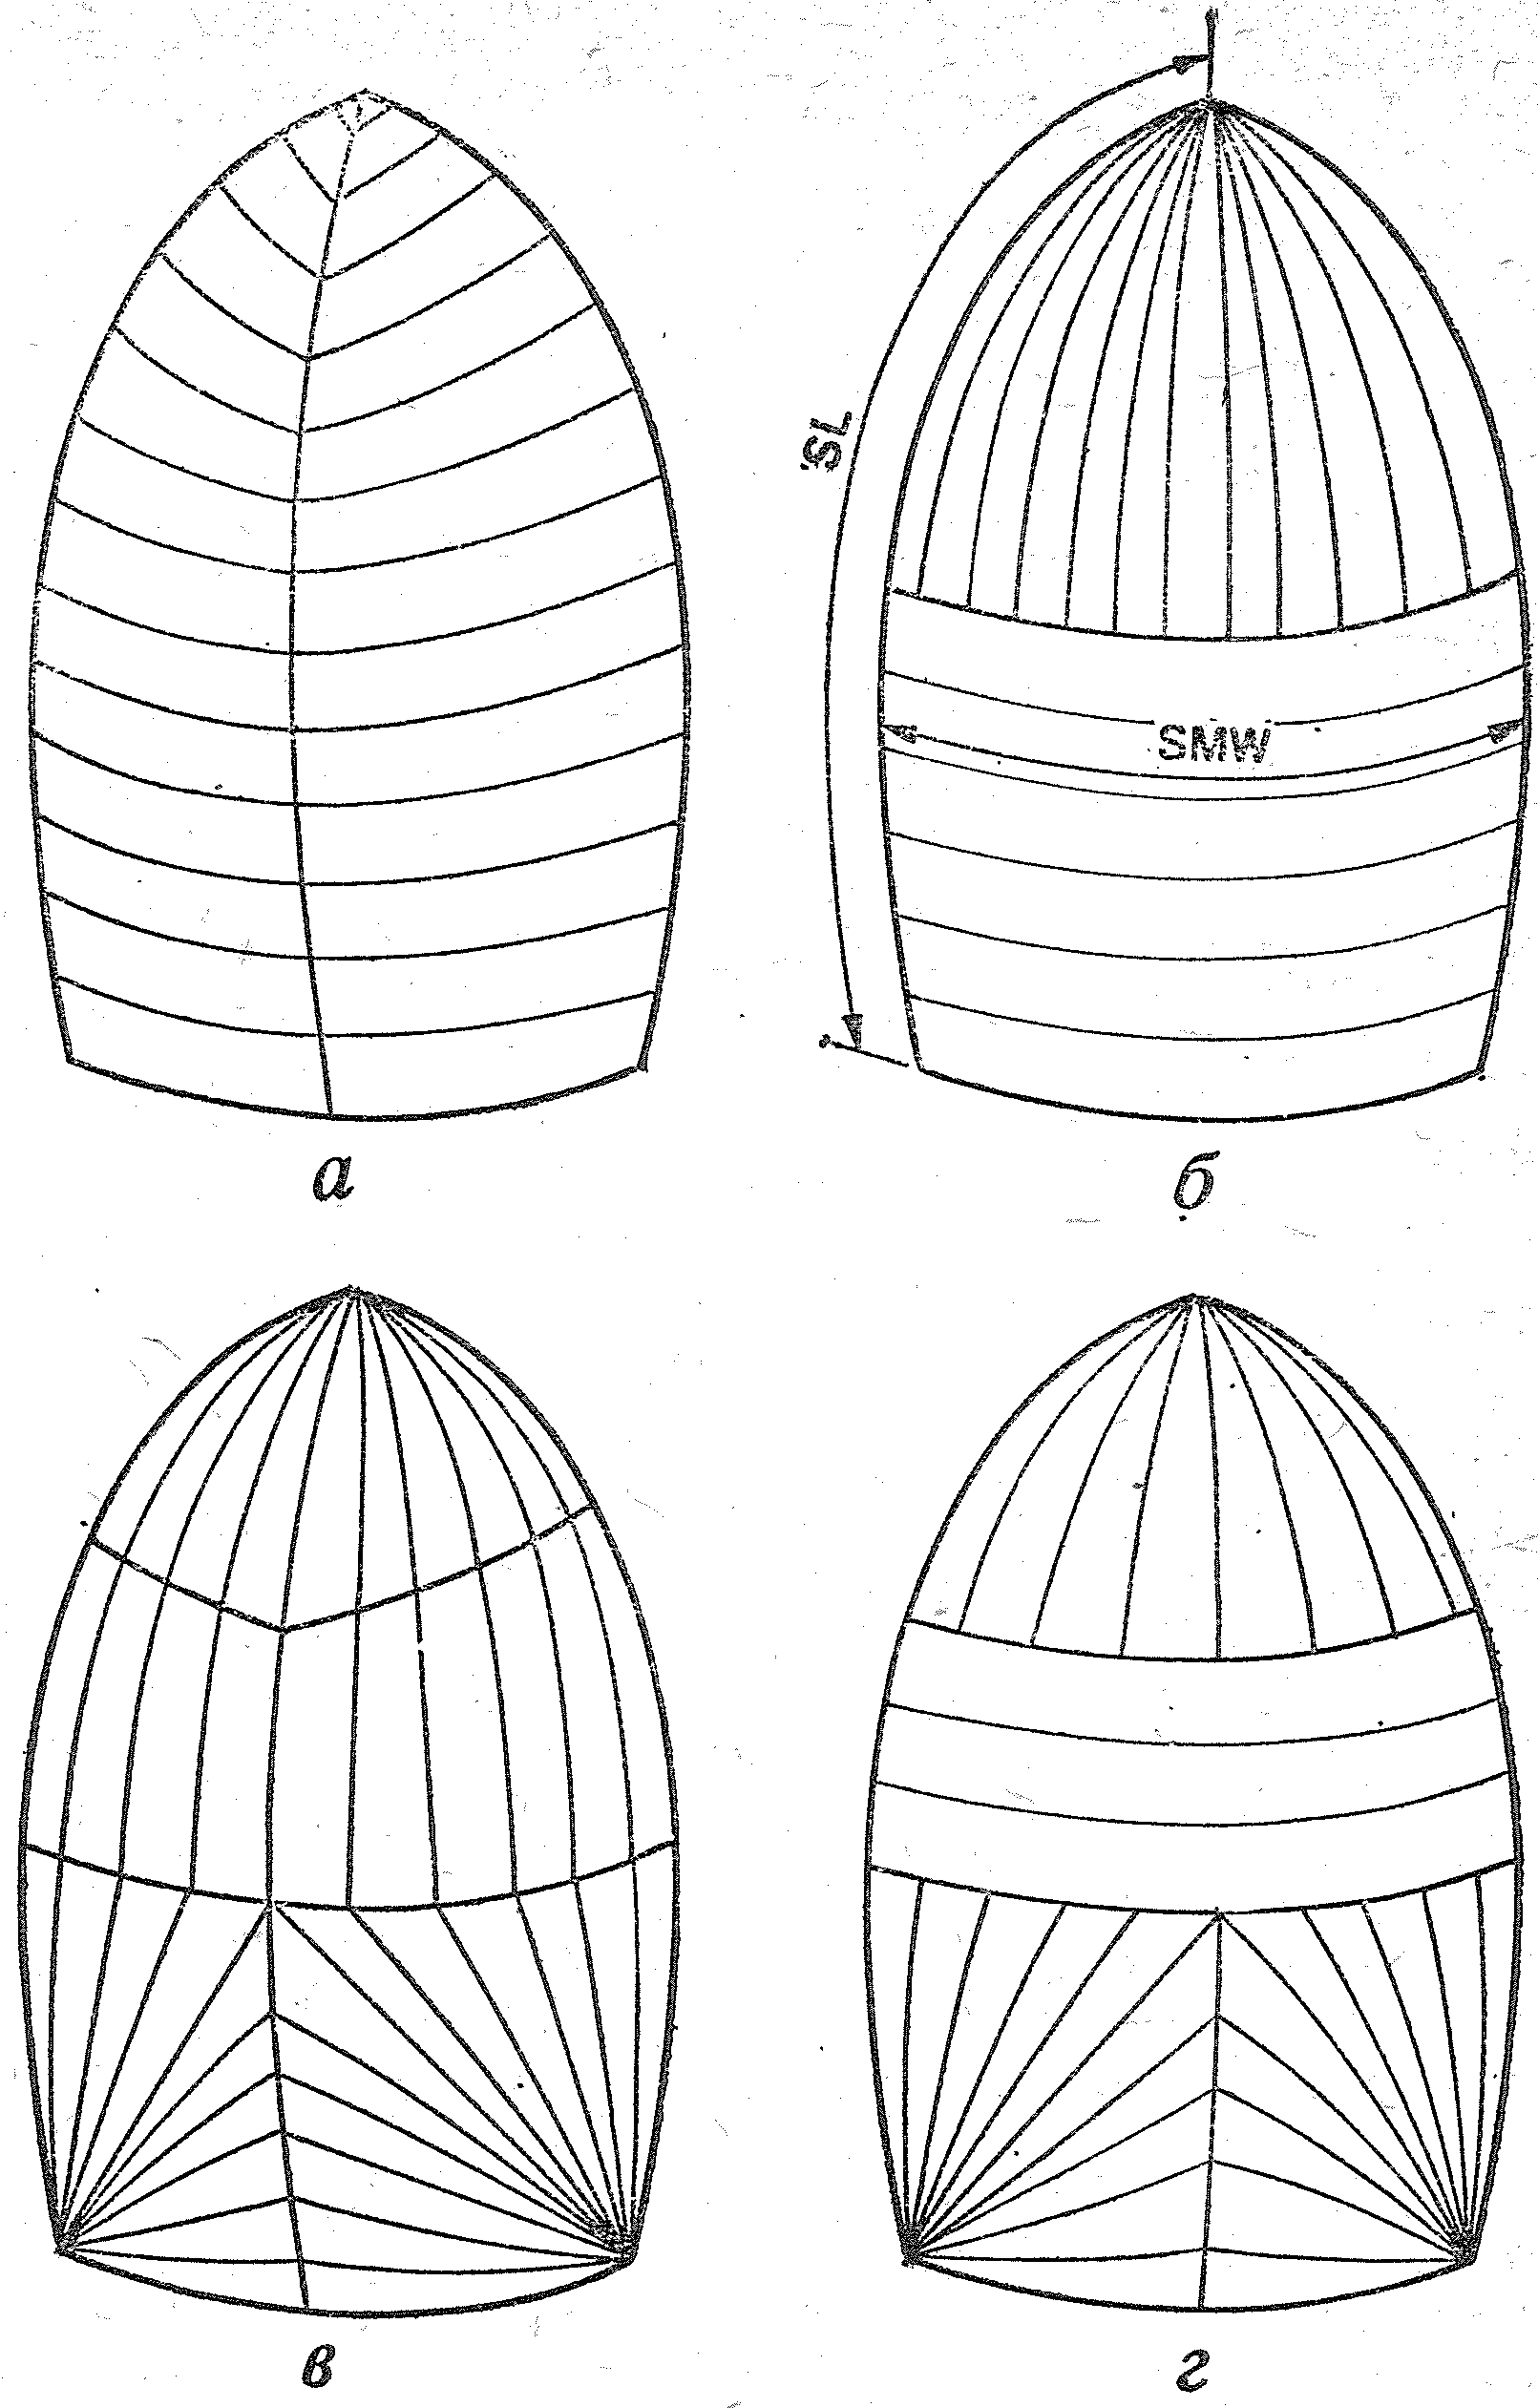
\includegraphics[scale=1.2]{0042P}
  \caption{Спинакеры}
  \label{fig:42}
  \small
  \centering{}
  Площадь сферического спинакера $S = 0,9 \cdot SL \cdot SMW$. Площадь <<звездного>> спинакера $ S = 0,74 \cdot SL \cdot SMW$
\end{figure}

\begin{figure*}[htb]
  \centering{}
  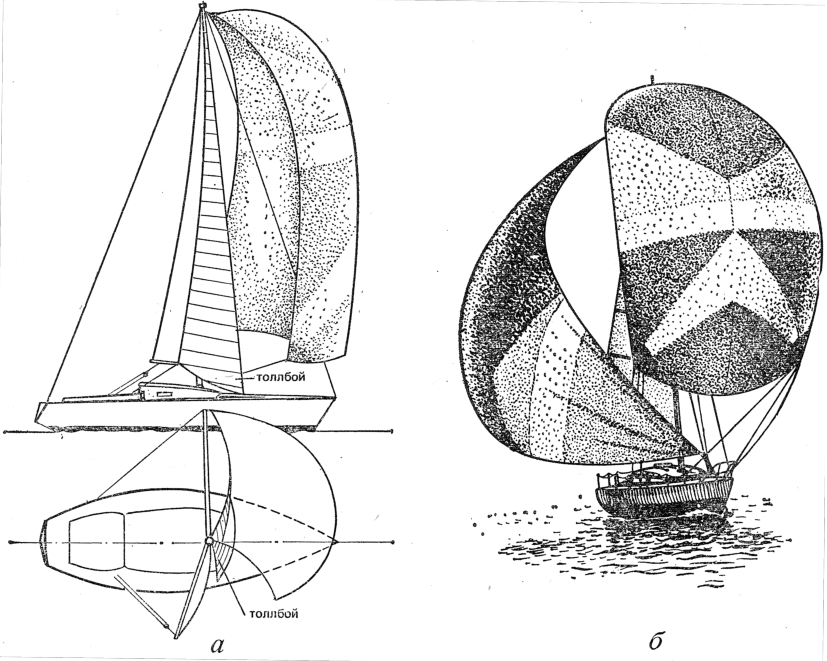
\includegraphics[scale=1.3]{0043P}
  \caption{Вспомогательные паруса для полных курсов}
  \label{fig:43}
  \small
  \centering{}
  \textit{а} \--- спинакер и толлбой; \textit{б} \--- спинакер и блупер
\end{figure*}

\begin{figure}[htb]
  \centering{}
  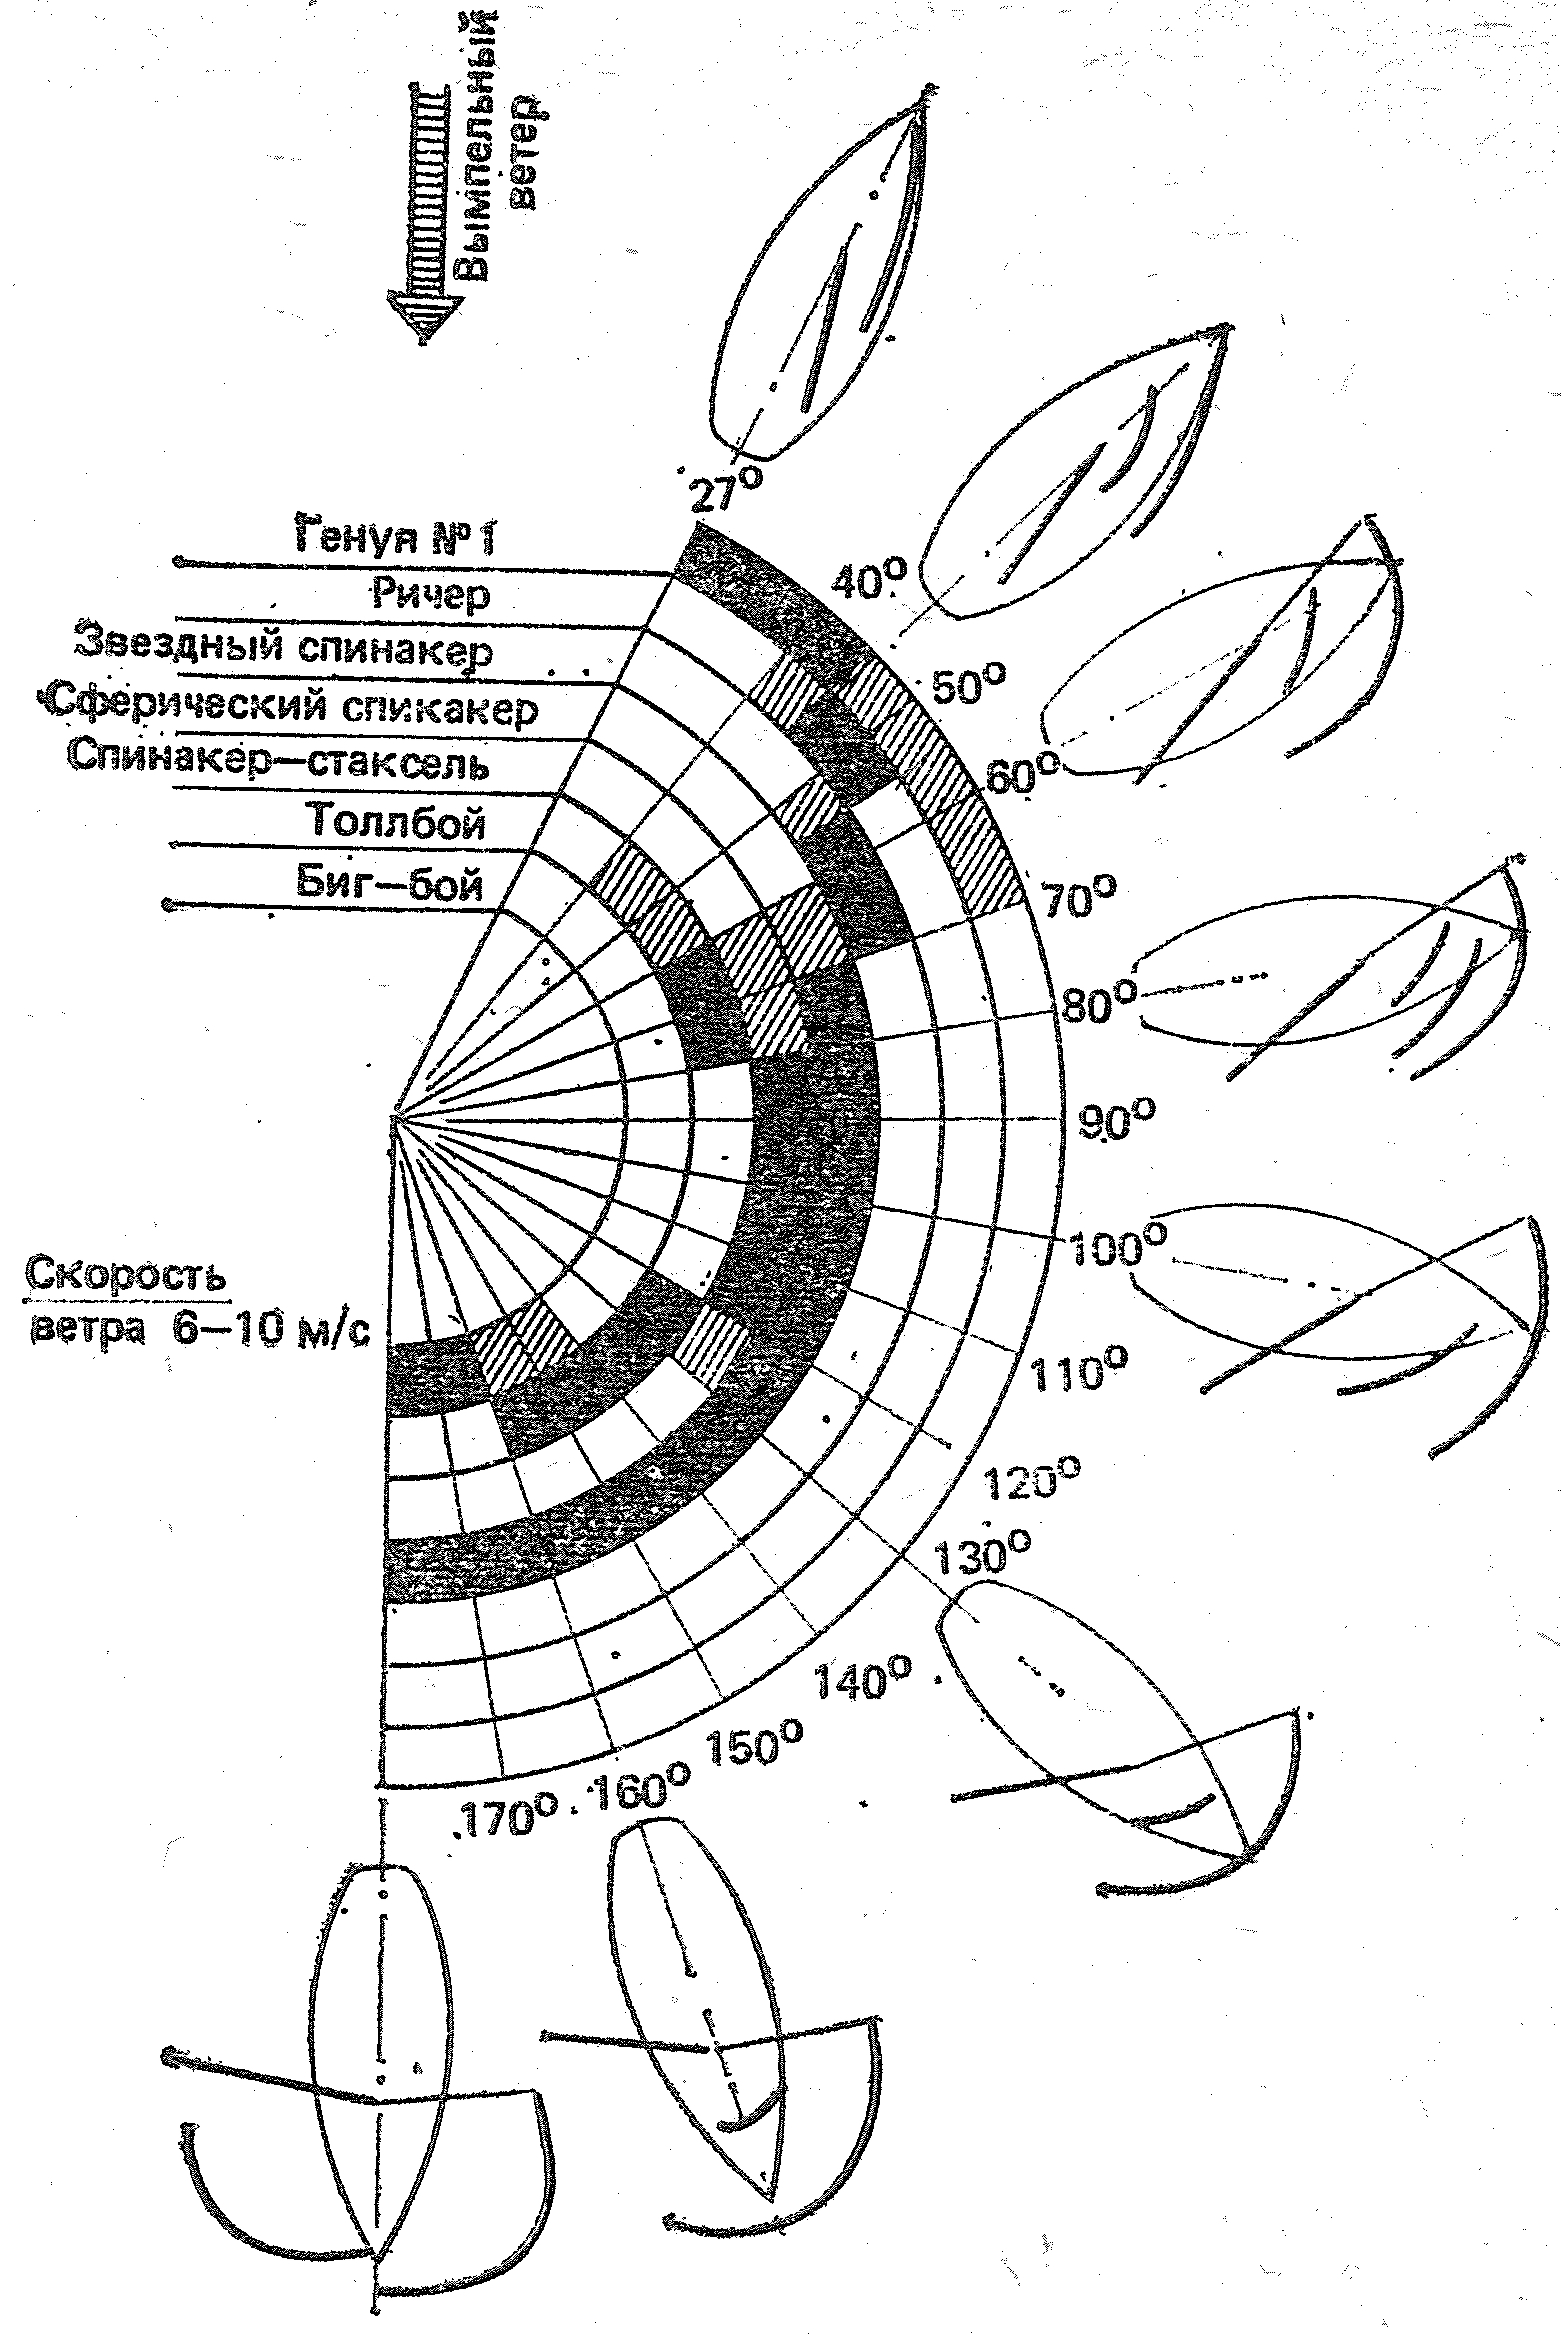
\includegraphics[scale=1.2]{0044P}
  \caption{Диаграмма применимости основных и вспомогательных парусов}
  \label{fig:44}
\end{figure}

\begin{figure*}[htb]
  \centering{}
  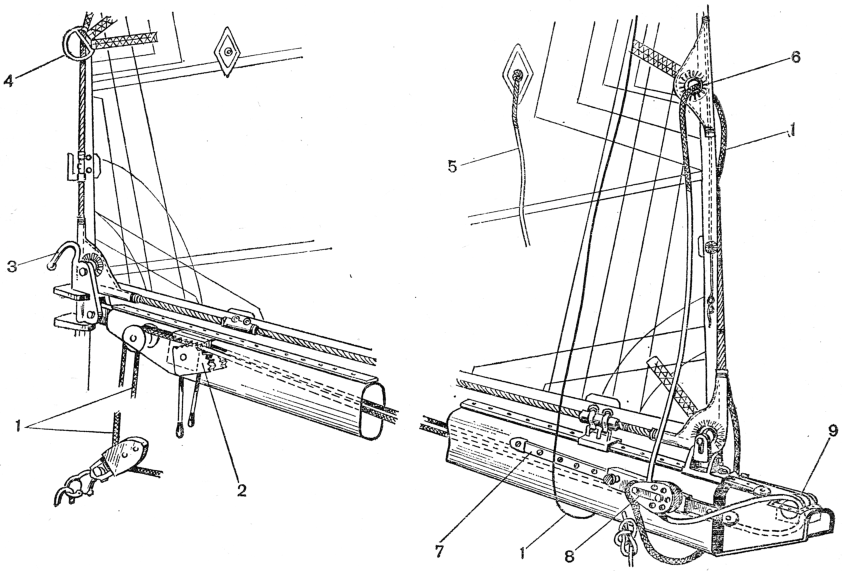
\includegraphics[scale=1.3]{0045P}
  \caption{Оснастка гика для взятия рифов}
  \label{fig:45}
  \small
  1 \--- риф-шкентели; 2 \---  стопора риф-шкентелей; 3 \--- крюк для закладывания кренгельса скобы; 4 \--- 5 \--- штерты; 6 \--- риф-кренгельс; 7 \--- рельс; 8 \--- блок риф-шкентеля на ползуне; 9 \--- врезные шкивы для шкентелей. 
\end{figure*}

\begin{figure}[htb]
  \centering{}
  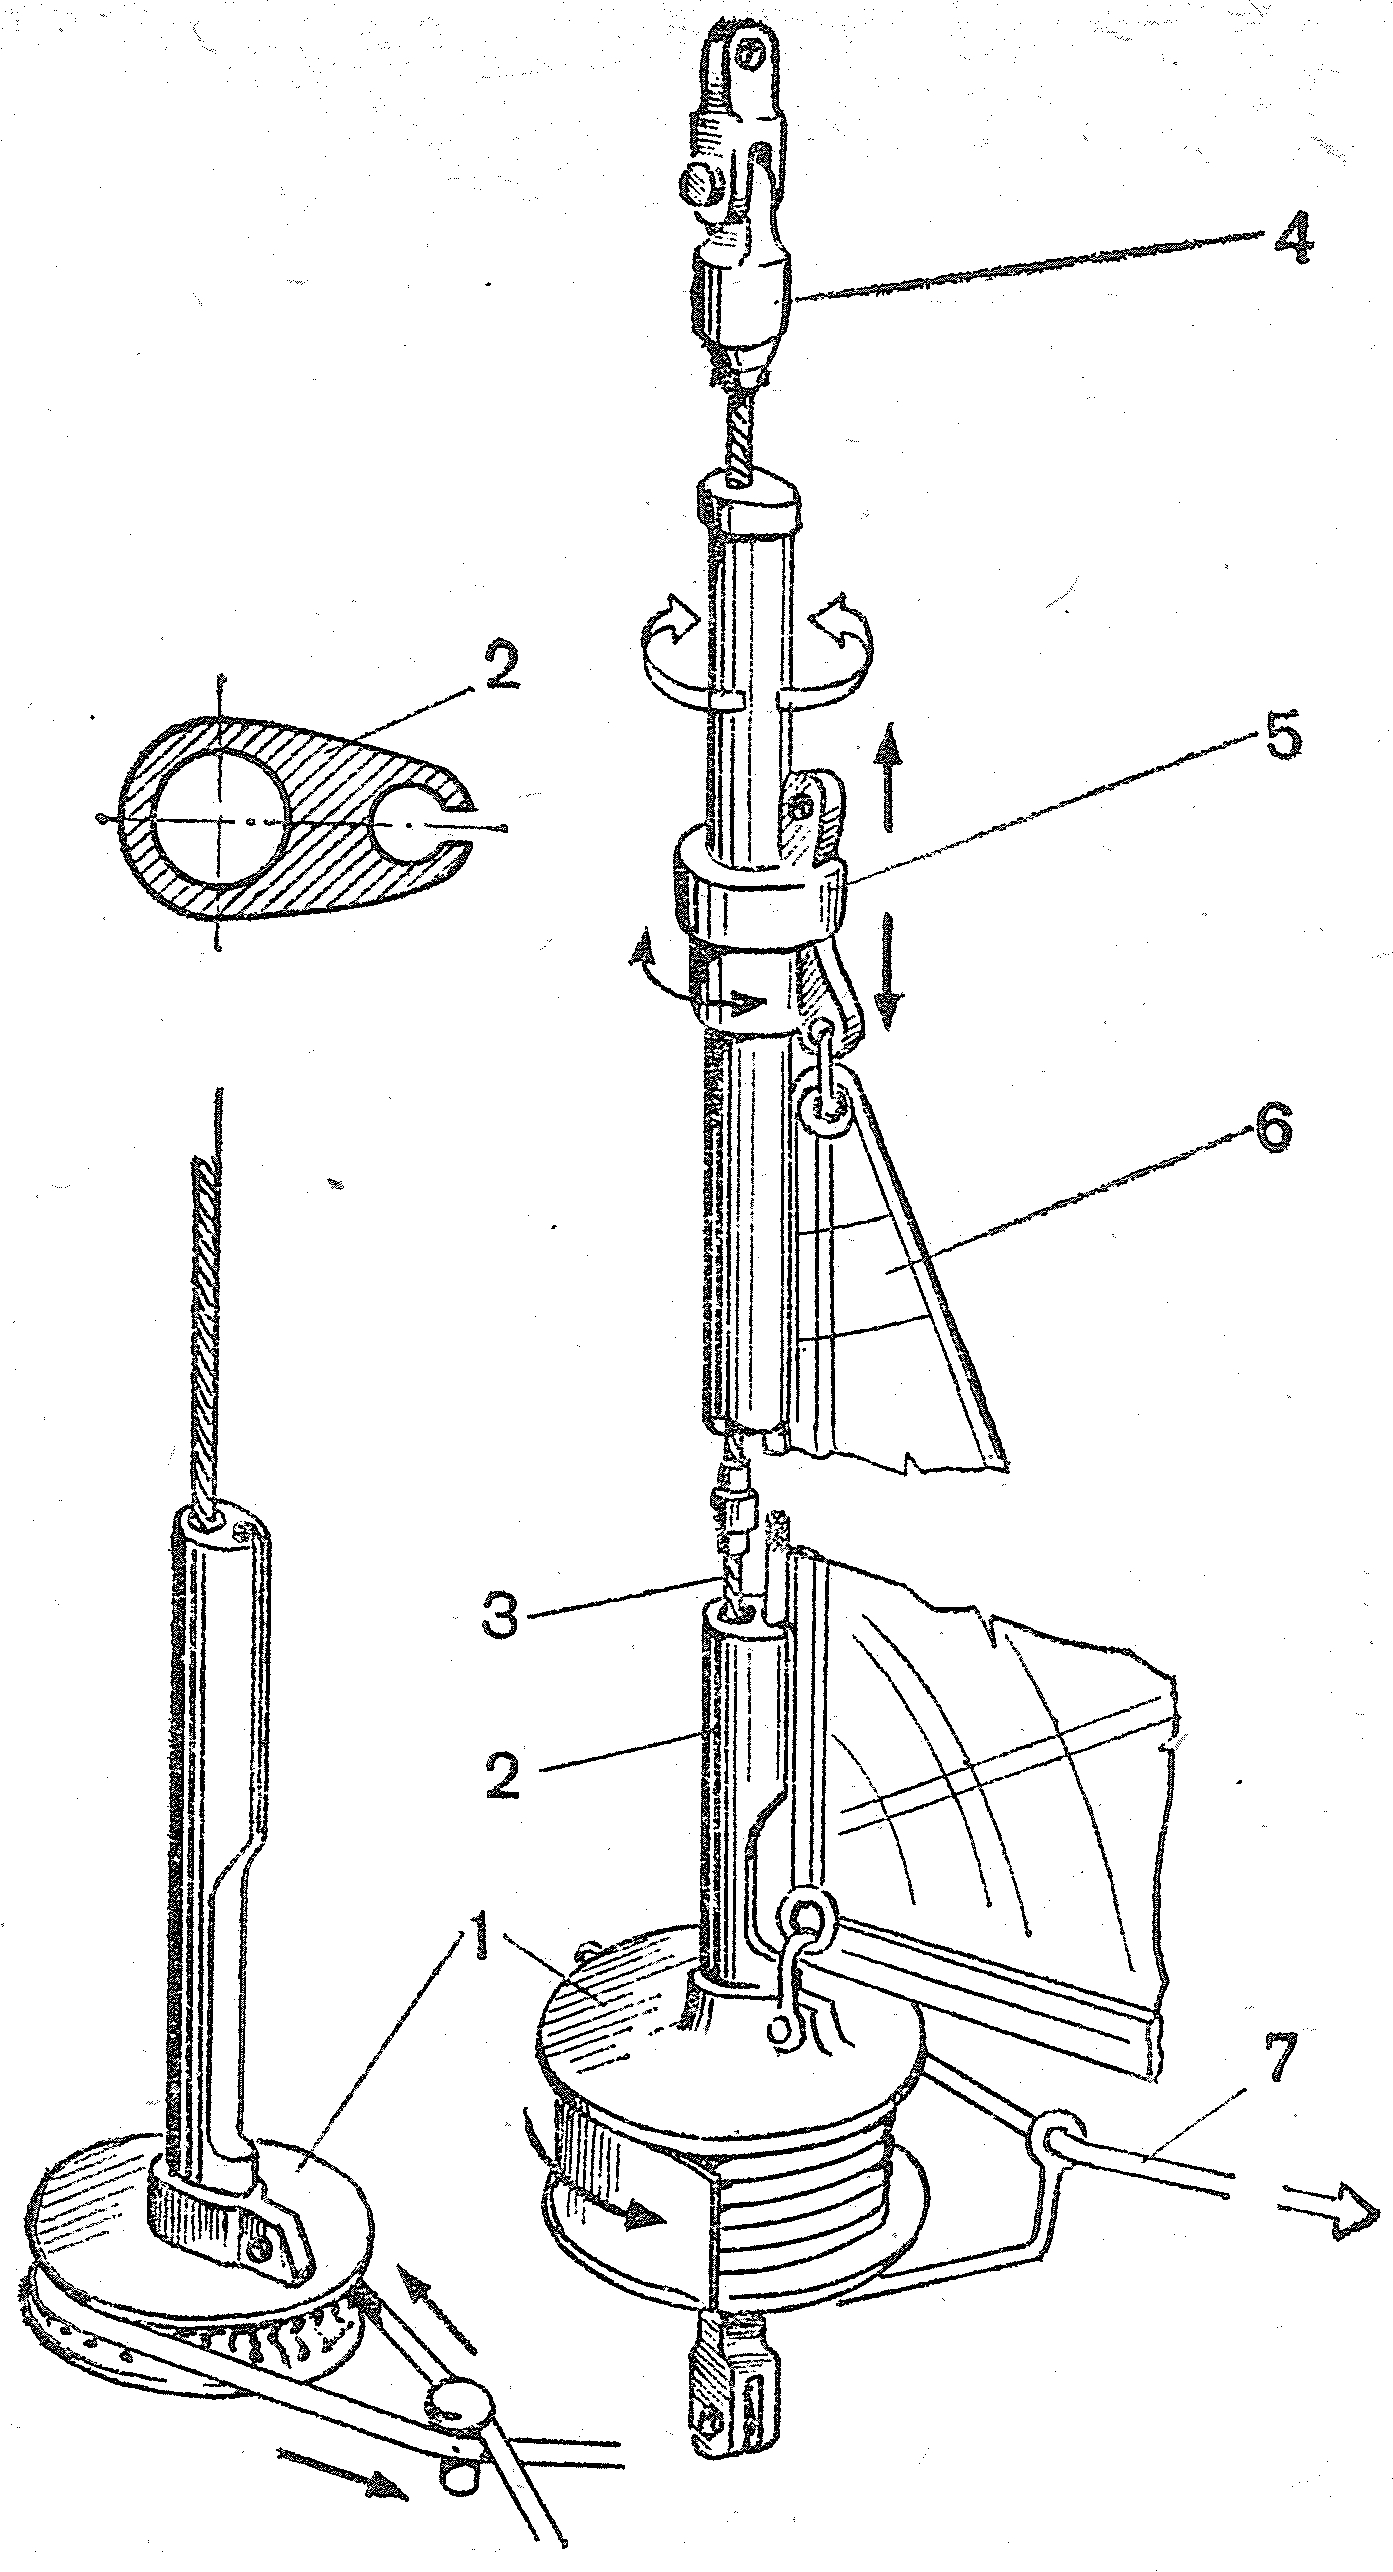
\includegraphics[scale=1.2]{0046P}
  \caption{Устройство для закрутки стакселя вокруг штага}
  \label{fig:46}
  \small
  1 \--- барабан; 2 \--- обтекатель; 3 \--- штаг; 4 \--- вертлюг; 5 \--- обойма для крепления фалового угла; 6 \--- парус; 7 \--- приводной трос
\end{figure}

При слабом ветре и на 70\gr ричер заменяют на \textbf{спинакер}. В свежий ветер (5 баллов) такая замена целесообразна уже при галфвинде, а в сильный (6\otdo 7 баллов) \--- при крутом бакштаге. 

По своей площади спинакеры являются самыми большими парусами, которые яхта может нести при ветре данной силы. Максимальная ширина спинакера по правилам IOR ограничивается величиной $1,8 \cdot I$, а длина боковых шкаторин $0,95 \sqrt{I^2 + IC^2}$, где $ІC$ \--- самый больший из следующих размеров: длина спинакер\-/гика, наибольшая ширина спинакера, деленная на 1,8, или $I$. Существует несколько разновидностей спинакеров, рассчитанных на разные условия плавания (рис.\ris{42}). 

\textbf{Сферический спинакер} (рис.~\ris{42}, \textit{а}) для слабого ветра шьется из самого легкого нейлона весом 30\gmsq. Выкраивается обычно из горизонтальных полотнищ, в верхней куполообразной части может иметь средний вертикальный шов. Для поддержания формы паруса при самых слабых дуновениях ветра должен иметь форму верхней части, приближающуюся к полусфере. Такой парус можно нести при ветре до 4 баллов и его курсовом угле до 60\gr.

\textbf{Радиальный спинакер} (рис.~\ris{42}, \textit{б}) в верхней части шьется из полотнищ, расходящихся лучами из фалового угла; в остальной части полотнища горизонтальны. Покрой этого спинакера более плоский, форма купола приближается к эллипсоиду. Материал \--- нейлон весом 50\otdo 60\gmsq; парус рассчитан на ветер от 3 до 6 баллов при курсовых углах от 180\gr до 60\gr. 

\textbf{Спинакер <<звездного>> покроя} (рис.~\ris{42}, \textit{в}) \--- очень плоский парус, предназначенный для несения, начиная от полного бейдевинда (до 45\gr). Его площадь превышает площадь самой большой генуи и дает преимущество при ветре от 2 до 6 баллов. Благодаря расположению полотнищ, расходящихся из всех трех углов, мало деформируется под нагрузкой и не увеличивает своей полноты при усилении ветра. Шьется из нейлона весом до 110\gmsq с максимально допустимой высотой, но узким. Иногда такие спинакеры называют спанкерами. 

Наконец, \textbf{штормовой спинакер} (рис.~\ris{42}, \textit{г}) для ветра свыше 12~м/с шьется из нейлона весом 110\gmsq с комбинированным или <<трирадиальным>> расположением полотнищ: горизонтальным в средней части и лучевым в каждом углу. Это препятствует сильному растяжению ткани, что дает парусу излишнюю полноту, которая приводит к образованию застойной зоны внутри спинакера и неустойчивости его работы. Этот парус имеет площадь, примерно равную 25\,\% площади наибольшего спинакера. 

Вместе со спинакером во время гонки яхта может нести дополнительные носовые паруса - толлбой (его назначение то же, что и в паре с генуей, рис.~\ris{43}), блупер и подспинакерный стаксель. 

\textbf{Блупер} (другие названия: шутер, бигбой, подветренный спинакер) \--- очень полно скроенный стаксель из легкого нейлона весом 65\gmsq с вогнутой передней и выпуклой нижней шкаториной, который по своим обмерам удовлетворяет правилам IOR для стакселей и может ставиться одновременно со спинакером на галсовой оковке для других носовых парусов. Главный эффект блупера \--- стабилизация яхты на курсе, так как он ставится по другую сторону от спинакера и противодействует его уваливающему действию. Кроме того, благодаря блуперу центр парусности перемещается вперед, умеряется раскачивание яхты, фаловый угол блупера \--- свободный, и фал служит таким же инструментом для управления парусом, как шкот и брас для спинакера. Блупер ставится при ветре от 3 до 13~м/с на курсах от полного бакштага до чистого фордевинда (160\otdo 180\gr).
 
Поскольку грот создает помехи для устойчивой работы спинакера и блупера, в свежий ветер и при спокойном море на нем берут риф, а в слабый ветер его лучше убрать совсем. 

При направлении ветра к курсу яхты под углом 135\gr и менее нести, блупер становится нецелесообразно и его заменяют толлбоем или подспинакерным стакселем.
 
Диаграмма, приведенная на рис.~\ris{44}, суммирует сказанное о применимости различных носовых парусов в средний ветер в зависимости от курса яхты относительно ветра. Залитые черным сектора обозначают рекомендуемый диапазон для несения паруса, заштрихованные \--- возможный.

Кроме основных и дополнительных парусов каждая яхта, участвующая в крейсерских гонках должна снабжаться штормовыми парусами \--- стакселем и триселем. 

\textbf{Бегучий такелаж.} Фалы парусов вырубают из гибких стальных тросов двойной свивки, изготовленных из нержавеющей или оцинкованной стальной проволоки. Используются тросы конструкции $7 \times 19$, состоящие из шести прядей по 19 проволок в каждой и такой же седьмой, служащей центральным сердечником, или $6 \times 19 + $\,ос \--- с сердечником из растительной пряди. Для надежности и долговечности фала важно, чтобы он имел достаточный запас прочности (не менее 4 и не менее 6 в тех случаях, если фал может быть использован для подъема человека на мачту) и был проведен через шкивы достаточно большого диаметра. Если трос огибает шкив под углом 180\gr, то диаметр шкива (по желобку для троса) не должен быть менее 20 диаметров троса. Если же направление тяги троса изменяется на 90\gr, то критическим будет диаметр шкива, равный 16 диаметрам троса. Огибая шкивы меньшего диаметра, проволоки троса подвергаются большим напряжениям снятия, и при повторяющихся на качке перемещениях фала по шкиву трос быстро изнашивается. Также важно, чтобы шкивы были изготовлены из более мягкого, чем сталь, материала \--- прочной пластмассы или бронзы. 

На топ мачты обычно проводится один грота\-/фал, два фала генуи и два спинакер\-/фала (обычно с вертлюжным блоком). Кроме того, на мачте может быть фал для стакселя, топенанта грота- и спинакер-гиков. При металлической мачте фалы проводятся внутри нее таким образом, чтобы исключалось переплетение отдельных тросов между собой. В нижней части мачты фалы выводят наружу и через направляющие футблоки проводят на лебедки шпилевого типа, обычно устанавливаемые впереди кокпита команды. 

Гика\-/шкот проводится даже крупных яхтах в 4 лопаря \--- необходимое усилие для добирания обеспечивается специальной лебедкой. Вместо двухшкивных предпочтительнее одинарные блоки, при которых трос не закручивается и легко травится без его раздергивания. Нижние блоки крепят к ползуну, перемещаемому по поперечному погону с помощью специальных талей. 

Для генуи часто применяют шкоты из стального троса, наращивая их на ходовых концах короткими отрезками синтетического троса для закладывания на барабан лебедки. Такие комбинированные шкоты хороши тем, что не вытягиваются в сильный ветер и позволяют сохранить угол атаки паруса при порывах ветра. Для спинакер\-/шкотов хорош полипропиленовый трос, который не намокает, а спинакер\-/брас лучше вырубить из стального тросика \--- он не вытягивается и позволяет сохранить оптимальную настройку спинакера при порывах ветра. 

Оттяжка гика в виде многократных талей на новейших яхтах заменяется винтовым или гидравлическим талрепом, что позволяет отказаться от проводки гика\-/топенанта. 

На рис.~\ris{45} представлена проводка бегучего такелажа для взятия рифов на гроте, а на рис.~\ris{46} \--- схема устройства для закрутки стакселя вокруг штага, снабженного обтекателем с ликпазом. На гоночных яхтах это устройство используется для временной уборки генуи при замене ее спинакером либо другим парусом, имеющим свободную переднюю шкаторину. Удобен также обтекатель штага с двумя ликпазами, который позволяет в спокойной обстановке поставить новый стаксель, а затем убрать предыдущий. 

В крейсерском плавании устройство для закрутки стакселя может быть использовано для уменьшения его площади, особенно если он скроен специально для этой цели плоским и с высоким шкотовым углом. Последнее позволяет при закрутке стакселя использовать одни и те же кипы стаксель\-/шкотов. 

\chapter{Правила обмера крейсерско-гоночных яхт}\label{chap:4}

Глава не публикуется, поскольку информация на данный момент устарела \--- рассмотрены правила IOR

\part{Яхтенное судовождение}

Судовождение --- прикладная наука, рассматривающая вопросы выбора кратчайшего пути судна и обсепечение его безопасности при плавании между заданными пунктами в море и между морскими портами. Судовождение состоит из четырех основных разделов: лоции, навигации (в том числе радионавигации и девиации магнитного компаса), астронавигации и навигационной гидрометеорологии. Здесь будут рассмотрены некоторые теоретические и основные практические сведения из этих разделов судовождения.

\chapter{Лоция}

\textbf{Морская лоция}\footnote{От голландского слова <<Loodsen>> \--- вести корабль.} родилась вместе с мореплаванием. В отличие от навигации или мореходной астрономии, основанных на математическом анализе, лоция носит описательный характер. Поэтому описание каждого конкретного океана, моря или их бассейнов также называется <<лоцией>>. В России первая лоция под названием <<Книга морская, зело потребная, явно показующая правдивое мореплавание на Балтийском море>> была издана в 1721~г. в Петербурге по указанию Петра~I.

Основная задача лоции \--- помочь мореплавателю избрать наиболее безопасный и выгодный путь для перехода морем. Для этого она дает штурману сведения об опасностях в море, системах ограждения этих опасностей, знакомит его с метеорологическими условиями в районе плавания, дает описание побережья и находящихся на нем портов, гаваней и бухт, указывает наиболее удобные курсы для переходов из порта в порт. Кроме того, лоция содержит все необходимые гидрологические и океанографические данные, характерные для описываемого района.

Обеспечение безопасности мореплавания возлагается на органы гидрографии. Так, в Великобритании этим занимается Гидрографический департамент Адмиралтейства, в Советском Союзе, \--- Главное управление навигации и океанографии Министерства обороны СССР (ГУНиО МО). Вместе с ГУНиО МО важную роль в обеспечении безопасности мореплавания играют специальные службы Министерства морского флота СССР \--- Главная морская инспекция, Гидрографическое предприятие, Службы безопасности мореплавания пароходств.

ГУНиО МО проводит научно\-/исследовательские работы в морях и океанах, собирает и систематизирует материалы для составления и корректуры морских карт и навигационных пособий, занимается ограждением морских опасностей, издает в качестве официальных пособий карты, лоции и другие руководства для мореплавания, а также систематически информирует мореплавателей об изменениях в навигационной обстановке по всем районам плавания.

В целях оказания помощи ГУНиО МО каждый судоводитель обязан немедленно сообщать его учреждениям о всех расхождениях карт, лоций и других пособий с действительностью: о вновь обнаруженных опасностях, об отсутствии на штатных местах знаков ограждения и случаях серьезных неувязок при определении места судна по береговым предметам, о желательности нанесения на карту тех или иных местных приметных береговых сооружений, облегчающих опознание берега и т.\=,д. 

\section{Терминология морской лоции}

Как и любая другая наука, лоция имеет свою терминологию. Ниже приводятся основные термины.

\textbf{Оборудованная береговая полоса.}

\begin{description}
\item [Порт] (\textit{port})\footnote{В скобках дается перевод терминов на английский язык} \--- место, закрытое от волнения, приспособленное для стоянки судов и имеющее средства для их разгрузки и погрузки, а также возможности для ремонта и снаряжения судов и обеспечения их необходимыми запасами (топлива, воды, продовольствия и пр.). Порты бывают военные, торговые и порты\-/убежища для стоянки во время шторма. 
\item [Рейд] (\textit{roadstead}) \--- любое пространство у берега, где судно может надежно встать на якорь. Рейд считается открытым, если он не защищен от ветра и волнения хотя бы с одного направления. Рейд, расположенный в хорошо защищенной бухте, называется закрытым. 
\item [Гавань] (\textit{harbour}) \--- часть акваторий порта или рейда, закрытая от волнения, течения и ледохода искусственными сооружениями. В гавани судно может стоять у берега (причальной стенки или пирса). 
\item [Бассейн] (\textit{dock basin}) \--- общее наименование части акватории гавани или порта, ограниченной причалами, пирсами, молами. Изолированные бассейны в портах со значительным колебанием уровня воды под влиянием приливов и отливов называются доками. Доступ в док осуществляется через ворота (батопорты) или шлюзы. 
\item [Аванпорт] (\textit{outer harbour}) \--- внешняя часть порта или гавани, защищенная от волнения молами, волноломами или имеющая естественное укрытие. Аванпорт обычно имеет большие глубины, чем основная часть порта. 
\item [Дамба] (\textit{dam}) \--- гидротехническое сооружение в виде насыпи или вала, служащее для предохранения берега от затопления или размывания, а также для защиты каналов, рейдов и устьев судоходных рек от наносов и волнения. 
\item [Мол] (\textit{mole}) \---оградительное сооружение в портах и гаванях, примыкающее одним концом к берегу. Конечная часть мола, выступающая в море, называется головой мола. 
\item [Волнолом] (\textit{breakwater}) \--- внешнее, не связанное с берегом, оградительное гидротехническое сооружение для защиты рейдов или гаваней от волнения. 
\item [Пирс] (\textit{pier}) \--- причальное сооружение для судов, одним концом примыкающее к берегу. 
\item [Причал] (\textit{berth}) \--- место для стоянки судов в порту, оборудованное причальными приспособлениями \--- палами, кнехтами, тумбами. 
\item [Пал] (\textit{pawl, bit}) \--- 1.~Деревянная свая или куст свай, забитых в грунт. 2.~Чугунная тумба на причале, на которую заводят швартовы. 
\item [Фарватер] (\textit{fairway}) \--- безопасный путь плавания судов среди различного рода препятствий, огражденный предостерегающими знаками. 
\item [Канал] (\textit{canal}) \--- искусственно прорытое русло для прохода судов через мелководье, обозначенное средствами навигационного оборудования. 
\end{description}

\textbf{Формы береговой черты.}

\begin{description}
\item [Бухта] (\textit{bay}) \--- небольшой залив. 
\item [Фиорд] (\textit{fiord}) \--- узкий глубокий залив или бухта, глубоко вдающиеся в гористые берега. 
\end{description}

\textbf{Навигационные опасности.}

\begin{description}
\item [Мель] (\textit{flat, ground}) \--- место, глубины над которым малы по сравнению с окружающими и поэтому опасные для мореплавания. 
\item [Отмель] (\textit{shoal}) \--- мель, простирающаяся от берега, с постепенно увеличивающимися глубинами. 
\item [Риф] (\textit{reef}) осыхающее или подводное возвышение морского дна со скалистым или коралловым грунтом; скопление камней, опасное для мореплавания. 
\item [Банка] (\textit{bank}) \--- отдельно лежащая мель, окруженная значительно большими глубинами. Считается безопасной для мореплавания, если глубина на ней более 20~м. 
\item [Бар] (\textit{bar of river}) \--- поперечная наносная мель в устьях рек или лежащая поперек входа в бухту. 
\end{description}

\textbf{Грунты.}

\begin{description}
\item [Глина] (\textit{clay}) \--- плотный грунт. Совокупность мелких частиц размером Менее 0,001~мм. Обладает вязкостью, якорь держит хорошо. 
\item [Ил] (\textit{mud, slime, ooze}) \--- совокупность частиц меньше 0,01~мм. Бывает плотный, вязкий и жидкий. Якорь держит в зависимости от степени плотности. Плохо держит жидкий ил (ооzе). 
\item [Песок] (\textit{sand}), \textbf{гравий} (\textit{gravel}), \textbf{хрящ} \--- совокупность частиц размером от 0,5~мм (песок) до 5,0~мм (гравий) и крупнее (хрящ). Держащая сила \--- в зависимости от плотности. Обычно средняя. 
\item [Плита, твердый грунт] (\textit{hard ground}) \--- массивные горные породы. Как грунт держит очень плохо. 
\end{description}

\textbf{Навигационное оборудование.}

\begin{description}
\item [Веха] (\textit{spar buoy}) \--- плавучий предостерегающий знак для ограждения морских опасностей в виде деревянного или металлического шеста с поплавком, топовой фугурой или без нее, установленный на якоре. Может быть снабжена радиолокационным (уголковым или спиральным) отражателем. 
\item [Буй] (\textit{buoy}) \--- плавучий предостерегающий знак для ограждения морских опасностей или фарватеров в виде металлического поплавка с фермой, устанавливаемый на якоре. Буи могут иметь устройства для подачи туманных сигналов и освещения в темное время суток, иногда снабжаются пассивными радиолокационными или оптическими отражателями. 
\item [Бакен] (\textit{beacon}) \--- в отличие от буя не имеет фермы и обычно не освещается. 
\item [Маяк] (\textit{light house}) \--- навигационный ориентир в виде башни отличительной формы и окраски, устанавливаемый на материке, острове или непосредственно на мелководье, оснащенный осветительным устройством с большой оптической дальностью видимости. 
\item [Плавучий маяк] (\textit{lightship}) \--- судно, оборудованное маячным огнем и устанавливаемое в районе удаленных от берегов опасностей или перед входом в морской порт (с функциями лоцманской станции). 
\item [Створ] (\textit{leading line}) \--- линия или вертикальная плоскость, проходящая через два ориентира (створных знака) и указывающая мореплавателям безопасное направление для движения судна. Задний знак при наблюдении с моря должен быть выше переднего (рис.~\ris{54}). Створы могут быть ведущими, по которым судно идет по заданному направлению; секущими, обозначающими место изменения курса на фарватере; девиационными, используемыми при работах по уничтожению девиации или определении поправки компаса. 
\end{description}

Перечисленные термины являются общепринятыми и употребляются в специальной литературе и официальных изданиях. В тех случаях, когда какой\-/либо термин не совпадает с местным названием предмета, в лоциях данного района обязательно указываются эти различия. 

\begin{figure}[htb]
  \centering{}
  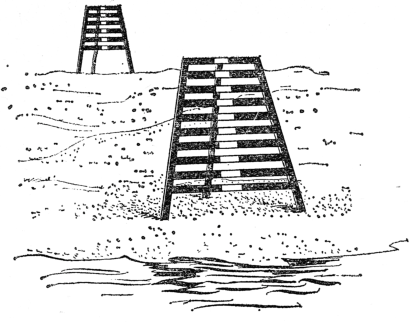
\includegraphics[scale=1.2]{0054P}
  \caption{Створные знаки}
  \label{fig:54}
\end{figure}

\section{Ограждение морских опасностей}

Для того чтобы обеспечить безопасность мореплавания, необходимо гогблюдать по крайней мере два условия: с достаточной точностью нанести на навигационную карту все известные морские опасности и оградить эти опасности в море определенными, хорошо видимыми знаками или другими искусственными предметами, по которым мореплаватель мог бы легко ориентироваться и заблаговременно уклониться от встречи с опасностью. Кроме того, каждый мореплаватель нуждается в различных береговых и морских ориентирах для определения своего места в море, опознания побережья, подходов к портам и якорным стоянкам.

Совокупность всех средств и устройств, которые обеспечивают безопасность мореплавания в определенном районе или море, обозначают надводную или подводную опасность, дают возможность опознать открывающийся берег и определить место судна при плавании вблизи берегов, называся навигационным оборудованием данного района или моря в целом. По месту установки средства навигационного оборудования могут быть береговыми и плавучими.

Основное назначение навигационного оборудования-ограждение морских опасностей. Плавучее ограждение устанавливают на воде \--- это буи, баканы, вехи и плавучие маяки, которые служат для непосредственного предостережения штурмана о существующей в данном месте опасности (рис.~\ris{55}). Береговое ограждение \--- морские и береговые маяки, береговые знаки и башни, створные знаки \--- устанавливают на прибрежной полосе материков и островов. В некоторых случаях роль берегового ограждения выполняют нанесенные на карту различные приметные места и предметы \--- отдельные высоты, триангуляционные вышки, приметные здания (церкви, башни и т.д.). 

\begin{figure}[htb]
  \centering{}
  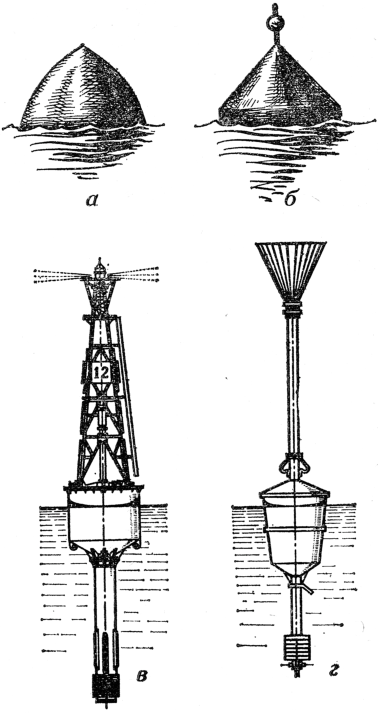
\includegraphics[scale=1.2]{0055P}
  \caption{Плавучее ограждение}
  \label{fig:55}
  \small
  \centering{}
  \textit{а, б} \--- Бакен; \textit{в} \--- буй; \textit{г} \--- веха
\end{figure}

По принятой в СССР единой системе ограждения, постоянные морские опасности делят на следующие группы:
\begin{enumerate}
\item Навигационные опасности 
  \begin{itemize}
  \item Естественные опасности (банки, мели, рифы, скалы и т.д.). 
  \item Кромки искусственных каналов и естественных фарватеров. 
  \item Затонувшие судна. 
  \item Районы свалки грунта. 
  \end{itemize}
\item Опасности ненавигационного характера: 
  \begin{itemize}
  \item Опасные из-за мин районы и фарватеры в них; 
  \item Запретные для плавания районы и полигоны. 
  \item Районы рыбной ловли. 
  \end{itemize}
\item Прочие ограждаемые районы: 
  \begin{itemize}
  \item Кабели и мерные линии. 
  \item Карантинные и якорные места. 
  \end{itemize}
\end{enumerate}

Существует две системы плавучего ограждения перечисленных опасностей: латеральная и кардинальная.

\textbf{Латеральная система} основана на принципе расположения предостерегательных знаков \--- буев, баканов, вех \--- справа или слева относительно сторон фарватера. Эта система применяется в основном при ограждении фарватеров, морских каналов, протраленных фарватеров в районах с минной опасностью, а также при ограждении судовых ходов на реках. Разновидностью латеральной системы можно считать ограждение широких фарватеров и рекомендованных курсов предостерегательными знаками вдоль осевой линии, дающее направление судну не <<между знаками>>, а <<от знака к знаку>>. Правая и левая стороны фарватера, обставленного по латеральной системе, определяются при следовании с моря (для морских и озерных фарватеров).

\textbf{Кардинальная система} \-- ее принцип основан на ограждении опасностей знаками, расставленными относительно сторон горизонта и указывающими мореплавателю, к какому из главных румбов (N, S, O или W) следует оставить буй или веху, чтобы миновать опасность. Эта система применяется при ограждении естественных навигационных опасностей, а также затонувших судов, запретных для плавания районов, районов свалки грунта, рыбной ловли и районов с минной опасностью. Все буи, как освещаемые, так и неосвещаемые, могут иметь и звуковые сигнальные устройства \--- колокола, ревуны, гудки. Эти устройства работают при волнении и служат для опознания буев в тумане. 

В водах Северо\-/Западной Европы с 1981~г. действует унифицированная система плавучих средств навигационного ограждения опасностей, которая в дальнейшем должна будет распространена на все районы Мирового океана. Эта система уже принята во всех государствах бассейна Северного моря, проливов Ла\-/Манш и Па\-/де\-/Кале, в Великобритании, Ирландии и на Атлантическом побережье Франции. Основана она на следующих принципах: 

\begin{itemize}
\item Возможность раздельного и совместного использования латеральной и кардинальной систем ограждения. 
\item Минимум числа плавучих знаков ограждения, их легкое и надежное опознание по цвету и характеру огня, без применения секундомера. 
\item На латеральных знаках огни зеленые и красные, на кардинальных \--- белые, с резко отличающимися характеристиками. 
\item Затонувшие суда ограждаются, как и все другие навигационные опасности, кардинальными или латеральными знаками. 
\item Новые опасности ограждаются по этим же правилам. Внешний вид унифицированных знаков показан в приложении \ref{app:2}, \textit{д}. 
\end{itemize}

В унифицированной системе наименование кардинального знака, как в большинстве стран мира, означает сторону, с которой судно должно пройти его. В водах СССР переход на новую систему ограждения намечено осуществить в течение пяти лет: в 1981~г. \--- на Балтийском море, в 1982-1983~гг. \--- на Азовском и Черном морях, в 1984~г. \--- в морях Дальнего Востока и в 1985~г. \--- в морях Северного Ледовитого океана.

Область применения плавучих маяков намного меньше, чем других плавучих предостерегательных знаков. Как правило, плавмаяки устанавливают в районах морских опасностей, значительно удаленных от берега при входе в проливы, каналы или теры (например, плавмаяк <<Рижский>> в Рижском заливе), часто качестве приемных маяков больших портов. Каждый плавучий маяк окрашивается приметным и отличным от краски других судов образом. Надводные борта плавмаяков обычнго окрашиваются в красный цвет. Вдоль обоих бортов большими буквами пишется название маяка. Плавучий маяк, находящийся на своем штатном месте, должен нести на топе мачты решетчатый шар, а ниже него \--- маячный флаг желтого цвета с прямым синим крестом. Сорванный со своего штатного места плавмаяк считается неработающим и вместо шара и маячного флага должен нести: днем \--- по одному черному шару в носу и корме (или по одному красному флагу) ночью \--- по одному красному огню на тех же местах. Плавмаяки могут так же подавать туманные и другие сигналы. В последнее время плавмаяки выходят из употребления и заменяются башенными морскими маяками.

Плавучее ограждение называется \textbf{штатным}, если оно нанесено на карты, Дополнительное ограждение, выставляемое для каких-либо специальных целей в летнее время, называется \textbf{летним}. \textbf{Зимнее} ограждение выставляется после ледостава в замерзающих портах для обозначения входа и выхода из портов, а также участков и рейдов для безопасного движения ледоколов и проводимых ими караванов. О выставлении летнего или зимнего ограждения сообщается в <<Извещениях мореплавателям>>.

\begin{figure}[htb]
  \centering{}
  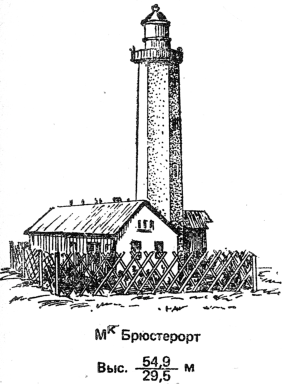
\includegraphics[scale=1.2]{0056P}
  \caption{Береговой маяк}
  \label{fig:56}
\end{figure}

\begin{figure}[htb]
  \centering{}
  \includegraphics[scale=1.2]{0057P}
  \caption{Морской маяк}
  \label{fig:57}
\end{figure}


\begin{figure}[htb]
  \centering{}
  \includegraphics[scale=1.2]{0058P}
  \caption{Береговой знак}
  \label{fig:58}
\end{figure}


Средства \textbf{берегового ограждения} \--- маяки, освещаемые и неосвещаемые знаки, створы и т.\=,д. \--- устанавливают для того, чтобы облегчить мореплавателям ориентировку в море относительно морских опасностей, лучше опознать берег и вход в порт или на рейд, определить место судна при плавании в видимости берегов Основным береговым ориентиром является маяк. Оснащенный мощным источником света, маяк в хорошую погоду ночью имеет дальность видимости до 15\otdo 20 миль и более. Мореплаватели относятся к сигналам маяков с самой высокой степенью доверия, так как местоположение их неизменно. 

В отличие от других навигационных знаков маяк обслуживает мореплавателей круглые сутки и в любую погоду. В зависимости от места установки береговые маяки делят на собственно береговые и на морские. 

\textbf{Береговые маяки} возводят обычно на высоких, выдающихся в море мысах материка или больших островов (рис.~\ris{56}), \textbf{морские} \--- на расположенных вдали от берега естественных или искусственных островках или просто на подводной скале (рис.~\ris{57}). По своему назначению береговые маяки могут быть опознавательными (указательными) и створными. Первые, как видно из названия, обычно служат приемными знаками при входе в какой-либо порт или канал (например, Дообский маяк при подходе к Новороссийску), поворотными знаками в том месте, где проходящие суда обычно меняют свой курс (например, Поворотный в Японском море), предостерегательными знаками, указывающими на определенную навигационную опасность (например, Родшер в Финском заливе). Створные маяки ставят для облегчения прохода судов в узкостях или входа на рейд, в гавань или в порт (например, Таллинские створные маяки).

Во избежание путаницы все маяки отличаются друг от друга не только внешним видом, но и характеристикой огня и туманного сигнала. Практически установлено, что маяки с одинаковой характеристикой не должны располагаться ближе чем в 80 милях друг от друга.

Главные требования к маякам сводятся к следующему: 

\begin{itemize}
\item Местонахождение каждого маяка должно быть точно нанесено на карту. 
\item Он должен быть хорошо виден и днем и ночью. 
\item Огонь маяка не должен приниматься за любой случайный огонь на берегу. 
\item Маяк должен иметь надежную туманную сигнализацию. 
\end{itemize}

Кроме маяков на берегу устанавливают освещаемые и неосвещаемые знаки. Освещаемые знаки отличаются от маяков меньшей величиной и тем, что на них ставят автоматические источники света, менее мощные и не требующие постоянного обслуживания. Неосвещаемые знаки служат ориентирами только в дневное время (рис.~\ris{58}). 

\section{Сигнальные и другие станции}

Кроме знаков плавучего и берегового ограждения безопасность мореплавания обеспечивает ряд специальных сигнальных станций, задача которых \--- передача на суда, находящиеся в море, сведений, имеющих значение для безопасного плавания. Они могут находиться при маяках или работать самостоятельно. К таким станциям относятся прежде всего радиостанции, которые в зависимости от своего назначения передают метеорологические сводки, радионавигационные извещения, сигналы времени и медицинские советы. Эти передачи ведутся по установленной программе, по запросу или в определенное время суток. 

\textbf{Телефонные станции} при маяках позволяют связать их с ближайшим портом или населенным пунктом.
Метеосводки и радионавигационные извещения (сокращенно МЕТЕО и НАВИМ) информируют мореплавателей об ожидаемой погоде и изменениях в навигационной обстановке. Их передают все береговые станции Министерства морского флота открытым текстом. Эти извещения могут быть очередными и срочными. Последние передаются немедленно по поступлении на радиостанцию, а очередные \--- по расписанию передач. Сигналы времени по радио даются в соответстви с программой, установленной данной станции, подробности о которой указываются в лоциях и в специальном издании <<Радиосигналы времени>>.

Кроме радиосвязи для передачи на суда нужной информации используются также звуковые, флажные (фигурные) и световые средства сигнализации. Для подачи таких сигналов на хорошо видном с моря месте устанавливают сигнальные посты, оборудованные мачтой, на которой поднимаю определенные сочетания флагов или фигур, обозначающих необходимы сигналы. В темное время суток эти сигналы передаются азбукой Морзе помощью клотикового фонаря или сочетаниями красного, зеленого и белого огней. С сигнальных постов обычно подаются следующие сигналы:
\begin{description}
\item [<<Предупреждение об опасности>>] \--- подается плавучими маяками, на мачте которых для судов, чей курс ведет к опасности, поднимается двухфлажный сигнал по Международному своду сигналов \--- <<Вы идете к опасности>> с одновременным пуском ракет (ночью сигнал дается только ракетами). Сигнал подается до тех пор, пока судно не увидит его и не изменит своего курса.
\item [<<Лоцманские сигналы>>] \--- они регулируют движение судов по каналу или фарватеру, сообщают о глубинах на фарватерах, о приливах и отлива в порту, о течениях и о высоте воды и т. п.
\end{description}

\textbf{<<Штормовые сигналы>>} \--- для предупреждения мореплавателей и населения портовых городов о надвигающихся штормах и сильных ветрах. Эти сигналы имеют значение для ограниченного района и служат в основной предупреждением для выходящих в море судов (см. приложение~\ref{app:2}, \textit{е}).

Туманные сигналы, имеющие весьма серьезное значение для безопасности плавания вблизи берегов, подают возушными и подводными средствами звуковой сигнализации при снижении видимости (туман, снежный заряд, морозь и т.\=,п.). В советских водах оздушные туманные сигналы подаются береговыми маяками при помощи следующих устройств: 

\begin{description}
\item [наутофон] \-- мембранный излучатель со звуком, напоминающим звук горна. Дальность слышимости достигает 3\otdo 4 миль; 
\item [сирена] \--- паровая или пневматическая с неподвижным или вращающимся рупором. Издает сильный воющий звук и имеет среднюю дальность слышимости 6\otdo 8 миль; 
\item [диафон] \--- издает сильный прерывистый звук, слышимый на расстоянии 6\otdo 8 миль;
\item [туманный горн] \--- имеет однотонный звук с небольшой дальностью слышимости (до 2 миль). Применяется в основном на плавучих маяках;
\item [свисток (или ревун)] \--- применяется на морских буях. Работает автоматически при волнении определенной силы;
\item [пушка] \--- выстрелы производятся с промежутком 10~мин. При ветре с моря выстрелы даются чаще;
\item [взрывы] \--- сильный звук от взрыва специального патрона на большой высоте; распространяется во все стороны и считается надежнее пушки;
\item [колокол] \--- в настоящее время применяется только на морских буях в качестве дублирующего средства на маяках.
\end{description} 

Береговые маяки подают двухударный звон с промежутком до 3 мин; плавучие маяки \--- трехударный звон с промежутком до 2 мин.

Отдельно могут быть выделены \textbf{радиопеленгаторные станции и радиомаяки}, которые, передавая определенные сигналы, служат для определения места судна в море при помощи радиопеленгов.

\textbf{Лоцманские станции} обеспечивают лоцманскую проводку судов в порт и из порта, а \textbf{спасательные станции} оказывают помощь судам, терпящим бедствие.

Все сведения о маяках, сигнальных станциях и передаваемых ими сигналах даются в <<Лоциях>> и отдельных изданиях <<Огни и знаки>> по каждому морю. В этих же изданиях имеются данные о лоцманских и спасательных станциях. Пункты, где имеются такие станции, обозначают на картах.

\section{Морские карты}\label{sec:maps}

\textbf{Морские карты} \--- основное пособие каждого штурмана. По своему назначению карты делятся на две основные группы: навигационные, непосредственно используемые в судовождении, и справочные \--- сборные листы, карты ветров, течений, часовых поясов, радиомаяков и т. д. К навигационным относятся следующие карты: 

\begin{description}
\item [генеральные (общие) карты,] которые имеют масштаб от 1\=,:\=,500\=,000 до 1\=,:\=,5\=,000\=,000 и служат для общего изучения изображаемых на них морей, океанов и их частей и для нанесения предварительной прокладки. На генеральных картах показывают только главные маяки и огни. Освещаемые буи и дневное плавучее ограждение наносят только у внешних опасностей и на подходах к портам. Изобаты нанесены по глубинам 20, 50, 100 и 200~м; 
\item[путевые карты,] масштаб которых от 1\=,:\=,100\=,000 до 1\=,:\=,500\=,000, служат для ведения навигационной прокладки и определения места судна с достаточной для мореплавания точностью. Внешние средства навигационного обеспечения наносят на этих картах полностью, а внутри рейдов и портов с большой разрядкой. Изобаты нанесены по глубинам 5, 10, 20, 50 и 100~м; 
\item[частные карты,] которыми пользуются для прокладки при плавании в непосредственной близости от берегов, в шхерах и узкостях и при подходе к берегу. Они имеют масштабы от 1\=,:\=,25\=,000 до 1\=,:\=,75\=,000. Изобаты нанесены по глубинам 2, 5, 10, 20, 50~м и все навигационные опасности с их береговым и плавучим ограждением; 
\item[планы] дают подробные изображения портов, бухт, гаваней, якорных стоянок и других ограниченных акваторий. Масштаб планов от 1\=,:\=,500 до 1\=,:\=,25\=,000. Все навигационные ограждения на планах наносят полностью. 
\end{description}

Для того чтобы правильно пользоваться картой, надо уметь читать ее, т.\=,е. понимать все нанесенные на карту условные обозначения и правильно разбираться в них. Чтение карты следует начинать с заголовка, в котором указывается ее название (район плавания), числовой масштаб с указанием главной параллели, к которой он отнесен, меры, в которых даны глубины и высоты прибрежных гор, а также год, к которому приведено магнитное склонение. После заголовка прочитывают расположенные под нижней рамкой отметки о датах последней (большой и малой) корректуры данной карты и год ее издания.
 
Все примечания, предупреждения (печатающиеся красным цветом), рисунки маяков и планы портов помещаются на карте таким образом, чтобы не закрывать береговой черты и водной поверхности. Адмиралтейский номер карты проставляется во всех четырех углах. С 1968~г. номера советских морских карт состоят из пяти цифр. Первая из них обозначает район Мирового океана, вторая \--- масштаб карты, третья \--- район океана или море, последние две цифры \--- порядковый номер карты данного района океана или моря. 

После предварительного знакомства с картой подробно просматривают район, в котором предстоит плавать, чтобы во всех подробностях изучить навигационную обстановку \--- глубины, опасности и систему их ограждения, береговую черту, расположение маяков и знаков. 

Для изображения на карте состояния и особенностей поверхности моря его дна и побережья применяется система условных обозначений, приведенная в приложении~\ref{app:2}, \textit{а}. 

\textbf{Глубины} на современных картах показываются в метрах и дециметрах. Точки с одинаковыми глубинами соединяются линиями равных глубин \--- изобатами. Изобата отделяющая прибрежное мелководье либо отдельную мель или банку, называется \textbf{линией опасности}, или \textbf{предостерегательной изобатой}. Для малых судов линией опасности считается 10-метровая изобата. 

Грунты обозначаются условными сокращениями, например: \textit{П} \--- песок, \textit{И} \--- ил, \textit{Кор} \--- кораллы и т.\=,д. Сложные грунты указывают сочетаниями сокращений составляющих грунтов: \textit{ИП} \--- илистый песок, \textit{ГрП} \--- гравий с песком, \textit{СрГл, МК} \--- серая глина, мелкий камень. Буквами обозначаются также цвет и характеристика грунта: \textit{жлП} \--- желтый песок, \textit{срмПГл} \--- серый мелкий песок с глиной. Если составляющие грунта располагаются слоями, то первым пишется верхний слой \textit{мППл} \--- мелкий песок на плите. 

\textbf{Естественные навигационные опасности} \--- банки, мели, рифы дают на картах контуром из точек с обязательным указанием наименьшей глубины над ними. Все остальные морские опасности обозначаются различными условными знаками. Если положение или существование показанной на карте опасности вызывает сомнения, то рядом с обозначением такой опасности или внутри нее ставятся пометки: \textit{ПС} \--- <<положение сомнительно>> или \textit{СС} \--- <<существование сомнительно>>. 

Места якорных стоянок обозначаются рисунком якоря. Изображение якоря без штока означает стоянку для малых судов, а якоря со штоком \--- для больших судов. Район с плохим грунтом обводят пунктиром с надписью: \textit{плх} (плохой грунт). 

Величина магнитного склонения указывается либо в заголовке карты, если она одинакова для всей карты, либо в центре картушки, расположенной на водной поверхности карты; центр картушки совмещается с точкой, где было определено склонение. В этой же картушке указывается годовое изменение склонения. Иногда величины склонений дают и без картушек. Так как картушки склонений имеют истинные направления, ими можно пользоваться вместо транспортира. Районы магнитных аномалий обводят сплошной толстой линией. 

Почти все средства навигационного оборудования имеют свои условные знаки. То, что не имеет своего знака, обозначается кружком с точкой в центре. Эта точка на карте соответствует точному местоположению знака на местности. Освещаемые знаки и маяки имеют на карте цветные изображения огней и их характеристики. Расцветка маячных огней показывается цветными окружностями с центром в точке нахождения маяка или частями окружности в пределах угла освещения. Характеристика огня дается рядом с маяком в одну строчку, например: \textbf{ГрПр(3)(25с)10М(н)}, что означает \--- группопроблесковый огонь с тремя проблесками и периодом 25~с, Дальность видимости 10~миль, туманный сигнал \--- наутофон. 

Направления, обозначающие граниты углов освещения маяков, на картах читаются от маяка в море. 

Створы обозначают на картах \textbf{сплошными линиями} (ходовая часть) и \textbf{пунктиром} (неходовая часть, а также поворотные и секущие створы на мерных линиях).

\textbf{Морские течения}, которые необходимо учитывать при прокладке, наносят на карты в виде стрелок: показывающие направление постоянного течения \--- с оперением, переменное \--- волнистой линией. Скорость течения с точностью до 1/4~уз пишется сверху стрелки. Приливные течения обозначают стрелкой с оперением сверху, отливные \--- без оперения (см. рис.~\ris{125}). 

Различные \textbf{приметные строения и предметы на берегу}, чье место определено, \--- церкви, башни, отдельные высоты, \--- также показывают условными знаками. Точное место показанного на карте предмета относится к середине основания или к центру условного знака. 

Представляющие для мореплавателя серьезную опасность \textbf{затонувшие суда} обозначаются пятью различными знаками: для затонувших судов с частями корпуса, возвышающимися над водой и представляющими явную опасность; с мачтами над водой; для судов, глубина над которыми меньше 18~м и больше 18~м; осыхающих. 

При подборе карт для плавания необходимо иметь в виду, что для прокладки следует использовать только карты самого крупного масштаба и откорректированные по день выхода в море. Корректура карт \--- это нанесение на нее тех изменений в морской и навигационной обстановке, которые произошли со дня ее издания: вновь обнаруженные опасности, упразднение одних знаков навигационной обстановки и открытие других, результаты новых промеров и т.\=,д., о которых должен знать мореплаватель. 

Большая корректура нужна при появлении новых гидрографических данных или накоплении большого числа малых корректур, которые существенно изменяют оригинал карты. Поэтому большая корректура проводится только картографическим производством \--- издаются новые исправленные карты. 

Малая корректура обычно предусматривает незначительные изменения. Ее выполняют от руки красными чернилами или тушью. Малая корректура карт, находящихся на складе гидрографии, производится работниками гидрографии, а карт, имеющихся на судах, \--- штурманами на основании <<Извещений мореплавателям>> (в плавании \--- по радиоизвещениям НАВИМ). Дата последней корректуры на получаемых из гидрографии картах должна быть указана под нижней рамкой карты со ссылкой на номера использованных <<Извещений мореплавателям>>. 

\section{Навигационные пособия}

Кроме морских карт в практике судовождения используют различные навигационные пособия, и в первую очередь <<Лоции>>, которые дополняют и уточняют сведения, данные на картах, облегчая тем самым решение навигационных задач. Кроме <<Лоций>> ГУНиО МО СССР издает и другие, вспомогательные, пособия: <<Каталог карт и книг>>, книги <<Огни и знаки>>, справочники <<Радиомаяки>>, различные таблицы и бланковые издания, в том числе и книгу <<Условные знаки морских карт и карт внутренних водных путей>>. 

\textbf{<<Лоции>>} издают отдельно для каждого моря или части океана. В общем случае каждая книга <<Лоции>> состоит из четырех основных разделов: 

\begin{enumerate}
\item \textbf{общий обзор}, в котором содержатся сведения о границах описываемого района, навигационно\-/географические и гидрометеорологические данные, сведения о портах и якорных стоянках, а также правила плавания в иностранных водах; 
\item \textbf{навигационное описание}, которое для удобства разделено по районам, и содержащее последовательно отдельные участки побережья, заливы, проливы, порты, фарватеры, приметные места, морские опасности, а также дающее наставления для плавания в различных местах, имеющих какие-либо особенности;
\item \textbf{справочный отдел}, где имеются таблицы расстояний между портами, словарь местных и иностранных слов и терминов, встречающихся в <<Лоции>> и на картах, и другие сведения; 
\item \textbf{алфавитный указатель}, содержащий географические названия всех портов, мысов, проливов, заливов, якорных стоянок и т.\=,п. Если <<Лоция>> охватывает иностранные воды, алфавитный указатель состоит из двух частей, в которых названия даются в русской и латинской транскрипции. 
\end{enumerate}

Кроме письменного материала <<Лоция>> содержит фотографии и рисунки приметных береговых мест и сборный лист карт данного района или моря. 

Так как срок службы <<Лоции>> около 10 лет, в течение этого времени периодически выпускаются дополнения и изменения, содержащие корректурный материал. Обязательным документом для корректуры <<Лоций>> являются также <<Извещения мореплавателям>>. Учет корректуры ведется на специальном листе, вклеенном в самом начале книги. 

<<Огни и знаки>> издаются чаще <<Лоций>> (через каждые 3\otdo 5~лет) и служат постоянным дополнением к ним. Их выпускают для каждого моря отдельно. Здесь есть все нужные штурману данные о маяках, освещаемых знаках, огнях и буях. Для получения этих данных надо найти в алфавитном указателе по названию маяка его номер, по которому и отыскивают сам маяк. О каждом маяке книга <<Огни и знаки>> сообщает следующие сведения: номер; название; положение (где находится маяк); широту и долготу с точностью до одной минуты; число, цвет, характер огня; дальность видимости огня (огней) в ясную погоду (в милях); высоту огня от уровня моря и от основания маяка (в метрах); описание маяка, его вид и окраску, высоту сооружения от его основания (в метрах); дополнительные сведения. 

Как и <<Лоции>>, книги <<Огни и знаки>> нуждаются в своевременной корректуре, основанием для которой служат <<Извещения мореплавателям>>. Кроме того, по мере накопления материала периодически издаются <<Дополнения к книгам ,,Огни и знаки''>>. 

<<Извещения мореплавателям>> \--- основные документы для корректуры карт и пособий \--- издают для всех морей Советского Союза и тех иностранных вод, которые охвачены советскими картами и пособиями, а также отдельно для районов плавания в советских водах, обслуживаемых Гидрографической службой флотов. Каждое <<Извещение мореплавателям>> имеет свой порядковый номер и ссылку на документ, по которому оно объявляется. 

Вспомогательным пособием для штурмана является <<Каталог карт и книг>>, который содержит подробные сведения о картах и навигационных пособиях и служит для подбора карт и пособий к предстоящему плаванию. Для того чтобы подобрать карту или <<Лоцию>>, пользуются сборными листами, помещенными в каталоге. 

<<Радиотехнические средства навигационного оборудования>> содержат сведения о морских радиомаяках и радионавигационных системах, о радиостанциях, передающих МЕТЕО и НАВИМ. 

Кроме этих пособий ГУНиО МО СССР издает также <<Мореходные таблицы>> (МТ) и <<Морские астрономические ежегодники>> (МАЕ), служащие для решения навигационных и астрономических задач.

\chapter{Практическая навигация}

Слово <<навигация>> произошло от латинского <<navigatio>> \--- судоходство. Судовождение является предметом штурманской специальности. От знаний и опыта штурмана зависит безаварийное плавание судна.

Штурманское дело на яхтах имеет ряд особенностей, осложняющих работу штурмана. К этим особенностям относятся: 
\begin{enumerate}
\item небольшая высота глаза над уровнем моря, что уменьшает видимость и усиливает влияние рефракции, искажающей формы предметов; 
\item ограниченный обзор, снижающий возможности наблюдения и пеленгования; 
\item значительные дрейф и рыскливость яхты на волнении и постоянный крен, которые вносят ошибки как в счисление, так и в обсервации; 
\item обычно слабая оснащённость техническими средствами судовождения. 
\end{enumerate}

\section{Форма и размеры Земли. Географические координаты} 

\begin{figure}[htb]
  \centering{}
  \includegraphics{N001}
  \caption{Эллипсоид вращения}
  \label{fig:N1}
\end{figure}

\begin{figure}[htb]
  \centering{}
  \includegraphics{N002}
  \caption{Географические координаты}
  \label{fig:N2}
\end{figure}

\begin{figure*}[htb]
  \centering{}
  \includegraphics{N003}
  \caption{Разность широт и разность долгот}
  \label{fig:N3}
\end{figure*}

В результате исследований установлено, что действительной формой Земли является геоид \--- неправильное геометрическое тело, близкое по форме к эллипсоиду вращения (сфероиду). Эллипсоид вращения образуется при вращении эллипса $P_NQP_SQ'$ вокруг его малой оси $P_NP_S$ (рис.~\ris{N1}). Разность между длинами большой и малой полуосей земного сфероида составляет только 21\=,382~м, т.\=,е. всего 0,3\,\% длины большой полуоси. Поэтому при решении большинства навигационных задач допустимо для упрощения всех расчетов принимать Землю за шар с радиусом 6\=,371,1~км., имеющий поверхность и объем почти одинаковые с земным эллипсоидом. 

Положение различных объектов на поверхности Земли может быть определено с помощью географических координат. Для отсчета координат на земной шар условно нанесена система точек и кругов (рис.~\ris{N2}). 

Введем ряд определений. Воображаемая прямая, вокруг которой происходит суточное вращение Земли, называется \textbf{земной осью}.

Точки пересечения ее с поверхностью Земли называются \textbf{географическими} или \textbf{истинными полюсами}: северным $P_N$ и южным $P_S$.

При сечении шара плоскостью получается круг, а на поверхности шара образуется окружность. Если секущая плоскость проходит через центр шара, то круг имеет наибольшие размеры и называется \textbf{большим}. Круги, образующиеся от сечения шара плоскостями, не проходящими через его центр, называются \textbf{малыми}. 

Окружность большого круга $QQ'$, плоскость которого перпендикулярна земной оси, называется \textbf{экватором}. Он делит земной шар на северное и южное полушария. 

Окружности малых кругов, плоскости которых параллельны плоскости экватора, называются \textbf{параллелями} ($pp'$). 

Окружности больших кругов, плоскости которых проходят через ось Земли, называются \textbf{географическими} или \textbf{истинными меридианами}. Половину окружности меридиана $P_NMP_S$, заключенную между полюсами и проходящую через данную точку $М$, называют \textbf{меридианом места}.

 Меридиан $P_NGP_S$, проходящий через астрономическую обсерваторию в Гринвиче (Англия), носит название \textbf{гринвичского} (начального) меридиана. Гринвичский меридиан вместе с противоположным ему меридианом $P_NG'P_S$ делит земной шар на \textbf{восточное} и \textbf{западное} полушария. 

В систему географических координат входят две сферические координаты: \textbf{широта} и \textbf{долгота}.

\textbf{Географической широтой} какой-либо точки называется угол при центре Земли, составленный отвесной линией (земным радиусом), проведенной через данную точку, и плоскостью экватора (угол $MOL$, см. рис.~\ris{N2}). Широта измеряется дугой меридиана от экватора до параллели данной точки. Она отсчитывается к северу или югу от экватора от 0 до 90\gr. Если точка находится в северном полушарии, ее широте приписывается наименование $N$ (северная), если в южном \--- $S$ (южная). Широту обозначают греческой буквой <<$\varphi$>>. 

\textbf{Географической долготой} какой-либо точки называется двугранный угол между плоскостью гринвичского меридиана и плоскостью меридиана данной точки (угол $GOL$, см. рис.~\ris{N2}). Долгота измеряется меньшей из дуг экватора между гринвичским меридианом и меридианом точки и отсчитывается от гринвичского меридиана к востоку или западу от 0 до 180\gr. Если точка находится в восточном полушарии, то долготе приписывают наименование $E$ (восточная), если в западном \--- $W$ (западная). Долготу обозначают греческой буквой <<$\lambda$>>.

\textbf{Разность широт} и \textbf{разность долгот}. Географические координаты судна в результате сделанного перехода изменяются. Изменения широты и долготы судна называются разностями широт и долгот. \textbf{Разность широт} (\textit{РШ}) двух точек на земной поверхности измеряется дугой меридиана, заключенной между параллелями этих точек. Наибольшее значение \textit{РШ} может составить 180\gr, что соответствовало бы перемещению судна из одного полюса в другой. Если судно перемещалось по какой-либо одной параллели, то \textit{РШ} равна 0\gr. Вычисленной \textit{РШ} приписывается наименование к $N$ или к $S$ в зависимости от того, в каком направлении перемещалось судно. Разность долгот (\textit{РД}) двух точек на земной поверхности измеряется меньшей из дуг экватора, заключенных между меридианами этих точек. Так как за разность долгот принимается всегда меньшая из дуг экватора, то ее значение не может превышать 180\gr. Если при сложении разноименных долгот получено значение, большее 180\gr, то за \textit{РД} принимается дополнение до 360\gr. Такой случай может возникнуть при пересечении судном меридиана 180\gr. Вычисленному значению \textit{РД} приписывается наименование к $E$ или $W$ в зависимости от того, в каком направлении перемещалось судно. Если северной широте и восточной долготе условно приписать знак <<плюс>> ($+$), а южной широте знак <<минус>> ($-$), то значение \textit{РШ} и \textit{РД} можно вычислить по алгебраическим формулам: 

\begin{gather}
  \text{\textit{РШ}} = \varphi_2 - \varphi_1\, ; \\
  \text{\textit{РД}} = \lambda_2 - \lambda_1\, ,
\end{gather}

где $\varphi_2$ и $\lambda_2$ \--- координаты конечной, а $\varphi_1$ и $\lambda_1$ \--- начальной точек плавания. 

Знак результата, полученного при вычислении по формулам, покажет наименования \textit{РШ} и \textit{РД}. Если при вычислении \textit{РД} берется дополнение до 360\gr, то наименование \textit{РД} меняется. Чтобы не ошибиться в значении и наименовании вычисляемых \textit{РШ} и \textit{РД}, следует хорошо представлять взаимное расположение меридианов и параллелей на земном шаре (см. рис.~\ris{N3}). На практике бывает нужно найти координаты точки, в которую пришло судно, если заданы координаты пункта отхода, а также \textit{РШ} и \textit{РД}, характеризующие положение точки прихода. Вычисления можно произвести по алгебраическим формулам:

\begin{gather}
  \varphi_2 =  \varphi_1 + \text{\textit{РШ}}\, ; \\
  \lambda_2 =  \lambda_1 + \text{\textit{РД}}\, ,
\end{gather}

где $\varphi_2$ и $\lambda_2$ \--- координаты конечной, а $\varphi_1$ и $\lambda_1$ \--- начальной точек плавания. 

\section{Единицы длины и скорости в судовождении}

За основную единицу длины, служащую для измерения расстояний в море, в судовождении принята морская миля. \textbf{Морской милей} называется линейное значение $1'$ дуги земного меридиана. Принято округленное значение средней величины морской мили, равное 1852~м. Кабельтов \--- единица длины для измерения небольших расстояний. Он равен одной десятой части мили. Округлённо кабельтов считается равным 185~м.
 
Глубины моря и высоты предметов на большинстве навигационных карт измеряются в метрах. На старых английских картах для указания высот предметов применялись футы (0,3048~м), а для указания глубин \--- футы и морские сажени (6~футов, или 1,83~м). Скорость судна при плавании в море измеряют узлами. 

Узел \--- это единица скорости, равная 1 морской миле в час, т.\=,е. 1,852~км/ч. 

\section{Основные линии и плоскости наблюдателя. Видимый горизонт наблюдателя и его дальность. Дальность видимости предметов и огней}

Для ориентирования в море принята система условных линий и плоскостей наблюдателя.

На рис.~\ris{N4} изображен земной шар, на поверхности которого в точке $M$ располагается наблюдатель. 

Его глаз находится в точке $A$. Буквой $e$ обозначена высота глаза наблюдателя над уровнем моря. 

\begin{figure}[htb]
  \centering{}
  \includegraphics{N004}
  \caption{Основные линии и плоскости наблюдателя}
  \label{fig:N4}
\end{figure}

Линия $ZMn$, проведенная через место наблюдателя и центр земного шара, называется отвесной или вертикальной линией. Все плоскости, проведенные через эту линию, называются вертикальными, а перпендикулярные ей \--- горизонтальными. 

Горизонтальная плоскость $HH'$, проходящая через глаз наблюдателя, называется плоскостью истинного горизонта наблюдателя. 

Вертикальная плоскость $VV'$, проходящая через место наблюдателя $M$ и земную ось, называется плоскостью истинного меридиана. 

В пересечении этой плоскости с поверхностью Земли образуется большой круг $P_NQP_SQ'$, называемый истинным меридианом наблюдателя. 

Прямая, полученная от пересечения плоскости истинного горизонта с плоскостью истинного меридиана, называется линией истинного меридиана или полуденной линией $N-S$. Этой линией определяется направление на северную и южную точки горизонта. 

Вертикальная плоскость $FF'$, перпендикулярная плоскости истинного меридиана, называется плоскостью первого вертикала. В пересечении с плоскостью истинного горизонта она образует линию $E-W$, перпендикулярную линии $N-S$ и определяющую направления на восточную и западную точки горизонта. 

Линии $N-S$ и $E-W$ делят плоскость истинного горизонта на четверти: $NE$, $SE$, $SW$ и $NW$. 

Плоскость истинного горизонта наблюдателя $HH'$ может быть представлена только в воображении. 

\begin{figure}[htb]
  \centering{}
  \includegraphics{N005}
  \caption{Видимый горизонт наблюдателя}
  \label{fig:N5}
\end{figure}

В открытом море наблюдатель видит вокруг судна водную поверхность, ограниченную малым кругом $CC_1$ (рис.~\ris{N5}). Этот круг называется видимым горизонтом наблюдателя. 

Расстояние $D_e$ от места судна $M$ до линии видимого горизонта $CC_1$ называется дальностью видимого горизонта. 

Теоретическая дальность видимого горизонта $D_T$ (отрезок $AB$) всегда меньше его действительной дальности $D_e$. Это объясняется тем, что из-за различной плотности слоев атмосферы по высоте луч света распространяется в ней не прямолинейно, а по кривой $AC$. В результате наблюдатель может видеть дополнительно некоторую часть водной поверхности, расположенную за линией теоретического видимого горизонта и ограниченную малым кругом $CC_1$. Этот круг и является линией видимого горизонта наблюдателя. 

Явление преломления световых лучей в атмосфере называется земной рефракцией. Рефракция зависит от атмосферного давления, температуры и влажности воздуха. В одном и том же месте Земли рефракция может меняться даже на протяжении одних суток. Поэтому при расчетах берут среднее значение рефракции. Формула для определения дальности видимого горизонта:

\begin{equation}
  D_e = 2,08 \sqrt{e} \, ,
\end{equation}

где $D_e$ в морских милях; $e$ \--- высота глаза наблюдателя над уровнем моря \--- в метрах.

В результате рефракции наблюдатель видит линию горизонта в направлении $AC'$ (см. рис.~\ris{N5}), касательном к дуге $AC$. Эта линия приподнята на угол $r$ над прямым лучом $AB$. Угол $r$ также называется земной рефракцией. Угол $d$ между плоскостью истинного горизонта $HH'$ и направлением на видимый горизонт называется \textbf{наклонением видимого горизонта}.  

Дальность видимого горизонта позволяет судить о видимости предметов, находящихся на уровне воды. Если предмет имеет определенную высоту $h$ над уровнем моря, то наблюдатель может обнаружить его на расстоянии: 

\begin{equation}
  D_N = D_h + D_e = 2,08 \sqrt{e} + 2,08 \sqrt{h} \, , 
\end{equation}

где: $D_N$ в морских милях, $e$ \--- высота глаза наблюдателя над уровнем моря \--- в метрах, $h$ \--- высота предмета над уровнем моря \--- в метрах. 

\begin{figure*}[htb]
  \centering{}
  \includegraphics{N006}
  \caption{Дальность видимости предмета}
  \label{fig:N6}
\end{figure*}

На морских картах и в навигационных пособиях приводится заранее вычисленная дальность видимости огней маяков $D_K$ с высоты глаза наблюдателя 5~м. С такой высоты $D_e$ равна 4,7 мили. При $e$, отличной от 5~м, следует вносить поправку. Её величина равна:

\begin{equation}
  \Delta D_K = 2,08 \sqrt{e} - 4,7 
\end{equation}

Тогда дальность видимости маяка $D_n$ равна: 

\begin{equation}
  D_n = D_K +  \Delta D_K 
\end{equation}

где: $D_n$, $D_K$ и $D_K$ в морских милях, $e$ \--- высота глаза наблюдателя над уровнем моря \--- в метрах.
 
Дальность видимости предметов, расчитанная по данной формуле, называется геометрической, или географической. Вычисленные результаты соответствуют некоторому среднему состоянию атмосферы в дневное время суток. При мгле, дожде, снегопаде или туманной погоде видимость предметов, естественно, сокращается. Наоборот, при определенном состоянии атмосферы рефракция может быть очень большой, вследствие чего дальность видимости предметов оказывается значительно больше рассчитанной. 

\section{Системы деления горизонта}

\begin{figure}[htb]
  \centering{}
  \includegraphics{N007}
  \caption{Системы деления горизонта}
  \label{fig:N7}
  \small
  \centering{}
  внутренний круг \--- румбовая; средний \--- четвертная; наружный \--- круговая
\end{figure}

Направления на поверхности Земли наиболее удобно определять путем измерения горизонтальных углов между плоскостью истинного меридиана наблюдателя и вертикальной плоскостью, проведенной, например, через тот или иной ориентир или совпадающей с диаметральной плоскостью судна. 

В эпоху парусного флота направления в море указывались в румбах (направлениях). По этой системе весь горизонт делится на 32 румба, из которых четыре отнесены к главным ($N$, $E$, $S$ и $W$), четыре \--- к четвертным ($NE$, $SE$, $SW$ и $NW$), восемь, расположенных между главными и четвертными румбами \--- к трехбуквенным ($NNE$, $ENE$, $ESE$ и т.\=,д.) и еще шестнадцать \--- к промежуточным румбам (рис.~\ris{N7}). Название трёхбуквенных румбов складывается из названий главных и четвертных, между которыми они находятся. Название промежуточных румбов состоит из названия ближайшего главного или четвертного румба, приставки <<тэн>> (ten), которая означает предлог <<к>>, и названия главного румба, в сторону которого уклонен данный промежуточный румб. Угол в 11\gr 1/4 между двумя смежными румбами также называется румбом. В каждой четверти горизонта румбы имеют порядковые номера от 1 до 8, причем нумерация румбов ведется от $N$ или $S$ в обе стороны: к $E$ и $W$. 

С появлением судов с механическими двигателями и повышением точности судовождения истинный горизонт стали делить на 360\gr, а счет направлений в румбах применять лишь для указания направления ветров, волнения и течения. Первоначально была введена четвертная система деления горизонта на градусы. За начало отсчета в ней принимаются два направления \--- $N$ и $S$, от которых счет ведется к $E$ или $W$ от О до 90\gr. В настоящее время в навигации принято отсчитывать направления только от $N$-й части истинного меридиана по часовой стрелке от 0 до 360\gr. Такая система деления истинного горизонта носит название круговой (см. рис.~\ris{N7}). 

\section{Истинные курсы и пеленги. Курсовой угол} 

\textbf{Путевым углом} называют двугранный угол между нордовой частью плоскости истинного меридиана и вертикальной плоскостью, совпадающей с линией перемещения судна. 

\begin{figure}[htb]
  \centering{}
  \includegraphics{N008}
  \caption{Изображение истинного курса, истинного пеленга и курсового угла}
  \label{fig:N8}
\end{figure}

Если на судно не влияет ветер, вызывающий дрейф и течение, линия перемещения судна совпадает с направлением его диаметральной плоскости. В этом случае направление движения судна определяется истинным курсом. \textbf{Истинным курсом} (\IK) называется двугранный угол между нордовой частью плоскости истинного меридиана и носовой частью диаметральной плоскости судна. 

Направление на ориентир определяется двугранным углом между нордовой частью плоскости истинного меридиана и вертикальной плоскостью, проходящей через место наблюдателя и ориентир. Этот угол называется \textbf{истинным пеленгом} (\IP). Оба угла отсчитываются от нордовой части истинного меридиана по часовой стрелке от 0 до 360\gr. Угол, отличающийся от \IP на 180\gr, называется \textbf{обратным истинным пеленгом} (\OIP): 

\begin{gather}
  \IP = \IK + \KU \\
  \IK = \IP - \KU \\
  \KU = \IP - \IK
\end{gather}

Если \KU задан по полукруговому счету, то \IP и \IK вычисляют по формулам: 

\begin{gather}
  \IP = \IK + \Kpb \text{\ или\ } \IP = \IK - \Klb \\
  \IK = \IP - \Kpb \text{\ или\ } \IK = \IP + \Klb 
\end{gather}

Когда \KU предмета равен 90\gr правого или левого борта, то говорят, что предмет находится на траверзе, указывая при этом наименование борта. 

\section{Земной магнетизм. Магнитное склонение. Магнитные курсы и пеленги} 

\begin{figure}[htb]
  \centering{}
  \includegraphics{N009}
  \caption{Магнитное поле Земли}
  \label{fig:N9}
\end{figure}

\begin{figure}[htb]
  \centering{}
  \includegraphics{N010}
  \caption{Магнитное склонение}
  \label{fig:N10}
  \small
  \centering{}
  $d_E$ \--- восточное; $d_W$ \--- западное
\end{figure}

\begin{figure*}[htb]
  \centering{}
  \includegraphics{N011}
  \caption{Зависимость между истинными и магнитными направлениями}
  \label{fig:N11}
\end{figure*}

В магнитном отношении Земля представляет собой огромный по величине магнит, магнитное поле которого окружает земной шар. Магнитные полюсы Земли располагаются сравнительно недалеко от географических, но с ними не совпадают. Кроме того, они постепенно изменяют свое положение. 

Силовые линии магнитного полюса Земли выходят из южного магнитного полюса $P_S$ и замыкаются в северном $P_N$ (рис.~\ris{N9}). 

Вертикальная плоскость, проходящая через ось свободно подвешенной магнитной стрелки, называется плоскостью магнитного меридиана, а след от пересечения этой плоскости с плоскостью истинного горизонта \--- магнитным меридианом $N_M - S_M$ (рис.~\ris{N10}). 

Горизонтальный угол, на который в данной точке Земли плоскость магнитного меридиана отклоняется от плоскости истинного меридиана, называется магнитным склонением $d$. Оно отсчитывается от северной части истинного меридиана $N_M$ к $E$ или к $W$ от 0 до 180\gr. Если северная часть магнитного меридиана $N_M$ отклонена от $N_M$ к востоку, то склонение имеет наименование $E$ (восточное) и ему приписывается знак плюс ($+$), если к западу, то $W$ (западное) со знаком минус ($-$). 

В отдельных точках Земли магнитное склонение отличается как по значению, так и по наименованию. В большей части судоходных районов склонение не превышает 25\gr $E$ или $W$. Исключением являются высокие широты, где склонение может достигнуть десятков градусов, а между одноименными магнитными и географическими полюсами даже 180\gr.

Чтобы правильно использовать магнитный компас, необходимо знать значение магнитного склонения в районе плавания. С этой целью на навигационные карты наносят значение и наименование склонения. Однако наблюдениями установлено, что значение склонения не остается постоянным даже в одном и том же месте. В отдельных районах за год склонение может изменяться до 0,2\otdo 0,3\gr. Поэтому на навигационных картах указывают также год, к которому отнесено склонение, и значение его годового изменения. Эти сведения наносят различными способами. Обычно надписи о значении склонения помещают в центре картушек, размещенных на водной поверхности. Иногда такие же надписи наносят на карту без изображения картушек, например <<Магн. скл. 1,2\gr $W$>>. Если значение склонения одинаково для всего района, охватываемого картой, то данные о нем помещают в заголовке карты. Значение годового изменения склонения обычно указывают в заголовке карты, однако, если оно неодинаково в разных районах карты, его показывают рядом со сведениями о значении склонения.  

Магнитное склонение, учитываемое при расчете поправки компаса, необходимо приводить к году плавания. Для этого к нанесенному на карте склонению прибавляют или вычитают из него годовое изменение склонения, умноженное на разность лет между годом фактического плавания и годом, к которому относится склонение на карте. Приведенные склонения при подготовке карт к предстоящему плаванию записывают простым карандашом рядом со старыми, которые зачеркивают. Если место судна находится в районе, расположенном между двумя обозначениями склонения, то нужное склонение определяют путем интерполяции. 

В наиболее изученных морях магнитное склонение известно с точностью до $\pm 0,5\gr$. В океанах, менее изученных в магнитном отношении, ошибки в выбранных значениях склонения могут достигать $\pm 1\motdo 2\gr$. В некоторых пунктах земной поверхности склонение резко отличается от его среднего значения для данного района моря или океана. Такое явление носит название магнитной аномалии. \textbf{Магнитные аномалии} возникают в местах, где под поверхностью Земли имеется скопление магнитных пород, создающих добавочное магнитное поле. Границы аномалий очерчены на морских картах кривыми чёрными линиями с указанием крайних пределов изменения магнитного склонения. При плавании в таких районах показания магнитного компаса ненадежны. Протекающие на Солнце явления могут вызывать внезапные и резкие изменения склонения и других элементов земного магнетизма. Продолжительность таких изменений составляет от нескольких часов до нескольких суток, их называют магнитными бурями. Во время магнитных бурь показания магнитных компасов ненадежны. 

Магнитным курсом называется угол в плоскости истинного горизонта, отсчитываемый от нордовой части магнитного меридиана по часовой стрелке до носовой части диаметральной плоскости судна; магнитным пеленгом называется угол в плоскости истинного горизонта, отсчитываемый от нордовой части магнитного меридиана по часовой стрелке до направления на ориентир (рис.~\ris{11}). Угол, отличающийся от \MP на 180\gr, называется обратным магнитным пеленгом (\OMP): $\OMP = \MP \pm 180\gr$ или $\MP = \OMP \pm 180\gr$. Магнитные курсы и пеленги могут лежать в пределах от 0 до 360\gr. Зная магнитное склонение в данном месте Земли, можно по известным магнитным направлениям получить истинные, а также решить обратную задачу. Зависимость между магнитными и истинными направлениями выражается формулами: 

\begin{gather}
  \IK = \MK + d \\
  \IP = \MP + d \\
  \OIP = \OMP + d 
\end{gather}

\begin{gather}
  \MK = \IK - d \\
  \MP = \IP - d \\
  \OMP = \OIP - d 
\end{gather}

Формулы алгебраические. Представляемое в них берется со знаком плюс ($+$) $E$ или минус ($-$) $W$. 

\section{Девиация магнитного компаса. Компасные курсы и пеленги} 

Находящиеся в магнитном поле Земли детали набора и другие стальные и железные части судна постепенно намагничиваются и приобретают свойства магнита. В результате этого в окружающем судно пространстве возникает собственное магнитное поле, действие которого складывается с магнитным полем Земли. Магнитная стрелка судового компаса устанавливается по равнодействующей сил обоих полей, вследствие чего отклоняется от направления магнитного меридиана. Горизонтальный угол, на который плоскость компасного меридиана отклоняется от плоскости магнитного меридиана, называется девиацией магнитного компаса <<$\delta$>> (рис.~\ris{12}). Девиация отсчитывается от северной части магнитного меридиана $N_K$ к $E$ (соответственно, со знаком $+$) или $W$ (со знаком $-$) от 0 до 180\gr. 

\begin{figure}[htb]
  \centering{}
  \includegraphics{N012}
  \caption{Девиация компаса}
  \label{fig:N12}
  \small
  \centering{}
  $\delta_E$ \--- восточная; $\delta_W$ \--- западная
\end{figure}

\begin{figure*}[htb]
  \centering{}
  \includegraphics{N013}
  \caption{Зависимость между магнитными и компасными направлениями}
  \label{fig:N13}
\end{figure*}

На каждом курсе девиация у судовых компасов различна. Это объясняется тем, что при изменении курса меняется положение судового железа относительно магнитных стрелок компаса. Кроме того, после поворота судна судовое железо частично перемагничивается, что также приводит к изменению магнитного поля судна. Девиация судовых компасов изменяется на одном и том же курсе при перемене широты места, что связано с изменением напряженности магнитного поля Земли и, следовательно, изменением намагниченности судового железа, а также при каждой погрузке или выгрузке грузов, обладающих магнитными свойствами, при длительной стоянке судна в ремонте, при проведении электросварочных работ вблизи компасов, при сильном сотрясении металлического корпуса судна. 

Девиацию судового компаса периодически определяют для различных курсов и заносят в специальную таблицу, откуда ее выбирают при расчетах курсов и пеленгов. Зная значение девиации, можно по замеченным компасным направлениям рассчитывать направления относительно магнитного меридиана. Компасным курсом (\KK) называется угол в плоскости истинного горизонта, отсчитываемый от нордовой части компасного меридиана по часовой стрелке до носовой части диаметральной плоскости судна; компасным пеленгом (\KP) называется угол в плоскости истинного горизонта, отсчитываемый от нордовой части компасного меридиана по часовой стрелке до направления на ориентир. Угол, отличающийся от \KP на 180\gr, называется обратным компасным пеленгом \OKP: 

\begin{gather}
  \OKP = \KP \pm 180\gr \text{\ или} \\
  \KP = \OKP \pm 180\gr
\end{gather} 

Компасные курсы и пеленги могут быть в пределах от 0 до 360\gr. Зависимость между компасными и магнитными направлениями: 

\begin{gather}
  \MK = \KK + \delta \\ \MP = \KP + \delta \\ \OMP = \OKP + \delta \\  
  \KK = \MK - \delta \\ \KP = \MP - \delta \\ \OKP = \OMP - \delta  
\end{gather}

Данные формулы алгебраические. Подставляемая в них девиация $\delta$ берется со знаком плюс ($+$) $E$ или минус ($-$) $W$.

Пользуясь этими формулами, можно рассчитать $\delta$ со своим знаком:

\begin{gather}
  \delta = \MK - \KK \\ \delta = \MP - \KP \\ \delta = \OMP - \OKP
\end{gather}

Между \KK, \KP и \KU ориентиров при круговом счете сохраняется следующая зависимость:

\begin{gather}
  \KP = \KK + \KU \\ \KK = \KP - \KU \\ \KU = \KP - \KK 
\end{gather}

\section{Определение остаточной девиации магнитного компаса. Таблица девиации} 

\begin{figure}[htb]
  \centering{}
  \includegraphics{N014}
  \caption{Определение девиации по створу}
  \label{fig:N14}
\end{figure}

Чтобы обеспечить надежную работу компасов, производят уничтожение их девиации при помощи магнитов девиационного механизма в нактоузе каждого компаса. Работа по уничтожению девиации проводится специалистами\-/девиаторами на оборудованных створами девиационных полигонах. Уничтожить девиацию полностью невозможно. Поэтому после проведения работ по уничтожению девиации девиатор приступает к определению остаточной девиации. Наблюдения проводят на створах, магнитное направление которых (\MP) известно, на восьми равноотстоящих курсах \--- главных и четвертных. В момент пересечения створа на каждом из восьми курсов берут по главному компасу \KP створных знаков (см. рис.~\ris{14}). Пользуясь соотношением $\delta = \MP - \KP$ девиатор вычисляет девиацию для восьми курсов, а затем рассчитывать таблицу остаточной девиации компаса с точностью до 0,1\gr обычно с интервалом в 10\gr или 15\gr. Полученные данные сводят в таблицу девиации. Аргументом для входа в таблицу (табл.~\ref{tab:N1}) служит \KK судна. 

\begin{table}[htb]
  \centering{}
  \begin{tabular}{r|r||r|r}
    \toprule
    $\delta \gr$ & \KK\gr & \KK\gr & $\delta \gr$ \\
    \midrule
    $+1,7$ & 360 &  0 & $+1,7$ \\
    $+1,7$ & 350 & 10 & $+1,7$ \\
    $+1,7$ & 340 & 20 & $+1,7$ \\
    $+1,6$ & 330 & 30 & $+1,8$ \\
    $+1,3$ & 320 & 40 & $+2,0$ \\
    $+1,0$ & 310 & 50 & $+2,1$ \\
    $+0,6$ & 300 & 60 & $+2,3$ \\
    0,0  & 290 & 70 & $+2,5$ \\
    $-0,5$ & 280 & 80 & $+2,6$ \\
    $-1,3$ & 270 & 90 & $+2,7$ \\
    $-2,0$ & 260 & 100 & $+2,6$ \\
    $-2,1$ & 250 & 110 & $+2,4$ \\
    $-2,3$ & 240 & 120 & $+2,0$ \\
    $-2,8$ & 230 & 130 & $+1,5$ \\
    $-2,9$ & 220 & 140 & $+0,8$ \\ 
    $-2,8$ & 210 & 150 & $+1,0$ \\
    $-2,4$ & 200 & 160 & $-0,7$ \\
    $-2,3$ & 190 & 170 & $-1,6$ \\
    $-2,0$ & 180 & 180 & $-2,0$ \\
    \bottomrule
  \end{tabular}
  \caption{Таблица девиации}
  \label{tab:N1}
\end{table}

\section{Поправка магнитного компаса. Исправление и перевод курсов и пеленгов}

Алгебраическая сумма девиации и магнитного склонения, на величину которой компасные направления отличаются от истинных, называется поправкой магнитного компаса: 

\begin{equation}
  \Delta \MK = \delta + d 
\end{equation}

Девиацию и склонение берут со своими знаками. 

\begin{figure*}[htb]
  \centering{}
  \includegraphics{N015}
  \caption{Зависимость между направлениями}
  \label{fig:N15}
  \small
  \centering{}
  \textit{а} \--- истинным и компасным; \textit{б} \--- истинным и гирокомпасным
\end{figure*}

Задачи, связанные с переходом от компасных курсов и пеленгов к истинным, называются исправлением румбов, а задачи, связанные с переходом от снятых с карты истинных кусов и пеленгов к компасным \--- переводом румбов. Формулы исправления румбов: 

\begin{gather}
  \IK = \KK + \Delta \MK \\
  \IP = \KP + \Delta \MK \\
  \OIP = \OKP + \Delta \MK 
\end{gather}

Формулы перевода румбов: 

\begin{gather}
  \KK = \IK - \Delta \MK \\
  \KP = \IP - \Delta \MK \\
  \OKP = \OIP - \Delta \MK
\end{gather}

\begin{figure}[htb]
  \centering{}
  \includegraphics{N016}
  \caption{Исправление курса}
  \label{fig:N16}
\end{figure}

Для контроля правильности решений навигационных задач бывает полезно сделать чертёж, чтобы представить себе все соотношения (рис.~\ris{N16}). 

\section{Общие сведения о картографических проекциях}

Если судно, совершая плавание между двумя пунктами, идет постоянным курсом, то оно пересекает все меридианы под одним и тем же углом. Линия, пересекающая все меридианы под постоянным углом, называется \textbf{локсодромией} (в переводе с греческого \--- <<кривой бег>>). На поверхности земного шара локсодромия изображается в виде спирали, стремящейся к полюсу, но никогда его не достигающей (рис.~\ris{N25}). 

\begin{figure}[htb]
  \centering{}
  \includegraphics{N025}
  \caption{Изображение локсодромии и ортодромии на поверхности Земли}
  \label{fig:N25}
\end{figure}

В частных случаях при плавании курсами 0 и 180\gr локсодромия совпадает с меридианом, а при плавании курсами 90\gr и 270\gr \--- с параллелью. 

Плавание по локсодромии, т.\=,е. постоянным курсом, удобно. Это упрощает работу судоводителя. Недостатком плавания по локсодромии является то, что она не является кратчайшим расстоянием между точками на земной поверхности. Кратчайшим расстоянием между данными пунктами на земной поверхности является меньшая дуга большого круга, проходящая через эти точки или \textbf{ортодромия} (в переводе с греческого \--- <<прямой бег>>). При небольших переходах разность в длине между локсодромией и ортодромией незначительна, ею пренебрегают и совершают плавание по локсодромии. 

Морские навигационные карты применяют для графического учета движения судна во время его плавания. Для этого на карте прокладывают локсодромические курсы судна и пеленги на различные ориентиры. 

Основные требования, предъявляемые к морской навигационной карте: 

\begin{enumerate}
\item линия курса и пеленгов должны изображаться прямыми линиями. Поэтому все меридианы на карте должны быть взаимно параллельны, чтобы прямая линия, изображающая линию курса судна, пересекала бы их под одним и тем же углом; 
\item карта должна быть равноугольной. Это значит, что углы и направления, измеренные на местности, должны соответствовать углам и направлениям на морской навигационной карте. 
\end{enumerate}

Из всех видов картографических проекций в судовождении находят наибольшее применение \textbf{меркаторская} и \textbf{гномоническая} (центральная). 

\begin{figure*}[htb]
  \centering{}
  \includegraphics{N028}
  \caption{Постороение меркаторской проекции}
  \label{fig:N28}
  \small
  \centering{}
  \textit{а} \--- сетка меридианов и параллелей; \textit{б} \--- меркаторская проекция
\end{figure*}

\textbf{Масштаб} карты определяется как отношение длины прямой между двумя точками на карте к действительному горизонтальному расстоянию между этими же точками на местности. Различают два вида масштаба: числовой (численный) и линейный.
 
\textbf{Числовой масштаб} \--- дробь, числитель которой единица, а знаменатель \--- число, показывающее, скольким единицам длины на местности равна одна единица на карте. 

\textbf{Линейный масштаб} может быть выражен числовым соответствием единиц длины (например, <<3 мили в 1 см>>) или графически. На морских картах линейный масштаб наносят на вертикальные рамки карты. 

При развертывании сфероидической поверхности Земли на плоскость возникают искажения, вследствие чего степень уменьшения изображения в разных частях карты различна. Другими словами, масштаб карты меняется при переходе от точки к точке. 

Масштаб, присущий данной точке карты, называется \textbf{частным}. В заголовках карт указывается числовой масштаб, близкий к среднему значению частных масштабов карт данного моря или района. Такой масштаб называется \textbf{главным}. Минута широты, т.\=,е. линейная величина 1 минуты дуги меридиана, представляет собой морскую милю. Морские мили будут изображаться на меркаторской карте разными по длине участками меридианов, увеличивающимися по мере удаления от экватора.

 Графическое изображение 1-й морской мили на меркаторской карте на данной широте называется \textbf{меркаторской милей}. Измерять расстояние на карте следует меркаторскими милями на соответствующей им широте. 

\section{Классификация морских карт по назначению. Содержание морских навигационных карт}

\begin{description} 
\item [Планы] (масштаб 1\=,:\=,500 \--- 1\=,:\=,25\=,000) предназначены для ориентировки при заходах судов на рейды, в порты, бухты и т.\=,д. 
\item [Частные карты] (масштаб 1\=,:\=,25\=,000 \--- 1\=,:\-,50\=,000) предназначены для плавания в районах, сложных в навигационном отношении: при проходе узкостей, в шхерах и непосредственно у берегов. 
\item [Путевые карты] (масштаб 1\=,:\=,100\=,000 \--- 1\=,:\=,500\=,000) используют для обеспечения плавания судна в значительном удалении от берегов, иногда вне видимости береговых ориентиров. Карты этого типа наиболее распространены. Как правило, на путевых картах ведется прокладка пути судна. 
\item [Генеральные карты] (масштаб 1\=,:\=,1\=,000\=,000 \--- 1\=,:\=,5\=,000\=,000) используют для ведения прокладки при плавании в открытом море в большом удалении от берегов, для общего изучения условий перехода и для предварительной прокладки. 
\end{description}

Побережья морей <<покрываются>> рядом морских карт, каждая из которых охватывает свой географический район. Для связи с соседними картами и сохранения непрерывности графического счисления пути судна соседние карты имеют <<находы>>, т.\=,е. взаимные перекрытия. 

Карты печатают на стандартных листах размером $75 \times 100$~см. Кроме того, они могут быть изданы на половине или четверти стандартного листа размерами соответственно $75 \times 50$ и $38 \times 50$~см. Если какая-то часть побережья не размещается в заданном масштабе на стандартном листе, дополнительно к оттиску карты может быть напечатан клапан на нестандартном листе. Клапан подклеивают к основному листу карты. Иногда клапан печатают на свободном месте непосредственно на карте. 

Морским картам присваивают пятизначные адмиралтейские номера. Каждая из цифр номера карты условно обозначает название океана или его части, тип карты в зависимости от ее масштаба, район океана или моря и порядковый номер карты в данном районе. Особые буквенные или цифровые обозначения вводят для справочных карт и карт специального назначения. 

Картографическая сетка морской карты заполняется в соответствии со своим назначением географическими и навигационными элементами содержания, надписями и элементами дополнительной характеристики. К географическим элементам содержания карты относятся изображения берегов океанов, морей, заливов, рельефа морского дна и суши, государственных границ, населенных пунктов. К навигационным элементам отнесены порты, средства навигационного оборудования, фарватеры, морские каналы, навигационные опасности, навигационные ориентиры, данные магнитного склонения и другие элементы карты, имеющие навигационный характер. Надписи \--- это заголовок карты, географические названия, различные пояснения и предупреждения, а также данные об издании и корректуре карты. К элементам дополнительной характеристики относятся врезки, т.\=,е. небольшие крупномасштабные планы или карты важных в навигационном отношении участков побережья, помещенные на свободных местах листа, таблицы со сведениями о приливах и течениях, рисунки маяков, знаков и т.\=,д.
 
Элементы содержания карт передаются условными знаками, символами изображения или схематическими рисунками объектов. Различного рода надписи на картах, относящиеся к цвету и характеру огней, наименованию грунтов и т.\=,д., дают в виде сокращений. Местоположение объектов, не выражаемых в масштабе карты, показывается условными обозначениями. Действительное место объекта при этом принимается в геометрическом центре знака, если он имеет правильную геометрическую форму, или в середине основания, если объект изображается несимметричным рисунком или знаком с широким основанием. 

Глубины приводятся к нулю глубин и даются в метрах и дециметрах, причем глубины от 0 до 5~м округляют с точностью до 0,1~м; от 5 до 20 м \--- до 0,2~м; 20 и более \--- до 1~м. Кроме нанесения отметок глубин, на картах проводят линии равных глубин \--- изобаты. Изобата 10~м считается предостерегательной для малых судов, а 20~м \--- для крупнотоннажных. 

Береговую линию в морях с приливами наносят на карту двумя линиями. Одна из них (основная) соответствует следу полной воды в сизигию, а другая \--- наинизшему уровню моря. Заключенная между этими линиями зона называется осушкой. В морях, где приливы не превышают 0,5~м, за береговую линию принимают урез воды при среднем уровне моря. 

Высоты маяков и знаков в морях, не имеющих приливов, даются над средним уровнем моря, а в морях со значительным приливом \--- над уровнем средней полной сизигийной воды. 

Средства навигационного оборудования (СНО) \--- маяки, светящие и несветящие знаки, знаки створов, радиомаяки, плавучие маяки, буи, вехи \--- показывают на картах внемасштабными условными знаками. Рядом с изображением светящих СНО с помощью сокращений надписывают их характер, количество проблесков или затмений, период дальность видимости огня, сведения о радиотехнических станциях, туманных сигналах, секторах освещения. Направления и сектора маяков дают истинные, считая с берега от 0 до 360\gr по часовой стрелке. Рядом с изображением несветящих знаков в виде дроби показывают их высоту от уровня моря (числитель) и от основания знака (знаменатель). Рядом с изображением буев указывают их окраску, звуковые сигналы, порядковые номера, данные о радиолокационном отражателе, а у светящих буев \--- также и характер огня. Через центры изображений створных знаков проводят створные линии, ходовую часть которых изображают сплошной линией, неходовую \--- пунктиром. 

Так как степень подробности изображения местности зависит oт масштаба карты, то из всех карт, имеющихся на данный район, всегда следует пользоваться картой самого крупного масштаба. Чтение карты начинают с ее заголовка, в котором указывают название изображаемого района моря, масштаб карты, сведения о нуле глубин, принятые единицы для указания глубин и высот предметов, данные о магнитном склонении. Затем должны быть прочитаны напечатанные на карте предупреждения и примечания, установлены даты издания, а также большой и малой корректур. Для получения возможно полного представления об изображенной на карте местности изучают все показанные на ней географические и навигационные элементы изображения. 

При плавании в сложных в навигационном отношении районах рекомендуется сделать подъем карты, т.\=,е. увеличить ее наглядность выделением наиболее важных элементов карты. Для этого, в частности, карандашом наносят дуги, соответствующие дальности видимости маяков, заштриховывают опасные сектора огней, проводят линии опасных пеленгов. Перед пользованием картой нужно оценить ее с точки зрения достоверности и полноты нанесенного на нее изображения. Чем позднее составлена карта, тем больше ей можно доверять. Об уровне современности карты судят также по датам ее нового издания, большой и малой корректур. Для оценки достоверности изображения рельефа дна устанавливают степень подробности промера. Хорошо обследованным районам моря соответствует на карте большая частота и равномерность нанесения глубин. Редко и неравномерно показанные глубины, белые пятна между ними являются признаком недостаточной изученности района. 

\section{Графические задачи, решаемые на морских картах}

Все построения в процессе графического счисления выполняют при помощи прокладочного инструмента: навигационного транспортира, параллельной линейки, циркуля\-/измерителя, чертежного циркуля с карандашом. Линии наносят простым карандашом и убирают мягкой резинкой. 

\textbf{Снять с карты координаты заданной точки.} Наиболее точно эту задачу можно выполнить с помощью циркуля\-/измерителя. Для снятия широты одну ножку циркуля ставят в заданную точку, а другую так подводят к ближайшей параллели, чтобы описанная циркулем дуга ее касалась. Не изменяя угла раствора ножек циркуля, подносят его к вертикальной рамке карты и ставят одну ножку на параллель, до которой измерялось расстояние. Другую ножку ставят на внутреннюю половину вертикальной рамки в сторону заданной точки и снимают отсчет широты с точностью до 0,1 наименьшего деления рамки. Долготу заданной точки определяют таким же образом, только расстояние измеряют до ближайшего меридиана, а отсчет долготы снимают по верхней или нижней рамке карты. 

\textbf{Нанести точку по заданным координатам.} Работу выполняют обычно с помощью параллельной линейки и циркуля\-/измерителя. Линейку прикладывают к ближайшей параллели и отодвигают одну ее половину до заданной широты. Затем раствором циркуля берут расстояние от ближайшего меридиана до заданной долготы по верхней или нижней рамке карты. Одну ножку циркуля ставят у среза линейки на тот же меридиан, а другой ножкой делают слабый укол также у среза линейки в сторону заданной долготы. Место укола и будет являться заданной точкой.

\textbf{Измерить расстояние между двумя точками на карте или отложить известное расстояние от заданной точки.} Если расстояние между точками небольшое и может быть измерено одним раствором циркуля, то ножки циркуля ставят в одну и другую точки, не меняя его раствора, приставляют к боковой рамке карты в той же примерно широте, в которой лежит измеряемое расстояние. Большое расстояние при измерении разбивают на части. Каждую часть расстояния измеряют милями в широте данного участка. Можно также раствором циркуля взять с боковой рамки карты <<круглое>> число миль (10, 20 и т.\=,д.) и сосчитать, сколько раз уложить это число по всей измеряемой линии. При этом мили снимают с боковой рамки карты примерно против середины измеряемой линии. Остаток расстояния измеряют обычным способом. Если нужно отложить от заданной точки небольшое расстояние, то его снимают циркулем с боковой рамки карты и откладывают на проложенной линии. Расстояние берут с рамки примерно в широте заданной точки с учетом его направления. Если откладываемое расстояние большое, то берут с рамки карты примерно против середины заданного расстояния 10, 20 миль, и т.\=,д. и откладывают нужное число раз. От последней точки отмеряют остаток расстояния.
 
\textbf{Измерить направление проложенной на карте линии истинного курса или пеленга.} Параллельную линейку прикладывают к линии на карте и приставляют к срезу линейки транспортир. Транспортир перемещают вдоль линейки до тех пор, пока его центральный штрих не совпадет с каким-либо меридианом. Деление на транспортире, через которое проходит тот же меридиан, соответствует направлению курса или пеленга. Так как на транспортире нанесены два отсчета, то при измерении направления проложенной линии следует учитывать четверть горизонта, в которой лежит заданное направление. 

\textbf{Проложить от заданной точки линию истинного курса или пеленга.} При выполнении этой задачи используют транспортир и параллельную линейку. Транспортир накладывают на карту так, чтобы его центральный штрих совпал с каким-либо меридианом. Затем транспортир поворачивают в ту и другую сторону до тех пор, пока с тем же меридианом не совпадет штрих дуги, соответствующей отсчету заданного курса или пеленга. К нижнему срезу линейки транспортира прикладывают параллельную линейку, и, убрав транспортир, раздвигают ее, подводя к заданной точке. По срезу линейки в нужную сторону проводят линию. Перенести точку с одной карты на другую. С карты снимают направление и расстояние до заданной точки от какого-либо маяка или другого ориентира, нанесенного на обе карты. На другой карте, проложив от этого ориентира нужное направление и отложив по нему расстояние, получают заданную точку. Эта задача является комбинированной.

\section{Графическое счисление пути судна}

Для того чтобы судить о безопасности плавания, ориентироваться в окружающей обстановке и правильно выбирать курсы для дальнейшего перемещения, судоводитель должен в любой момент знать положение своего судна. Для этого он ведет \textbf{навигационную прокладку}. 

Перед выходом судна в рейс под руководством капитана по картам и навигационным пособиям изучают условия плавания на всем предстоящем переходе. На основании этих данных выполняют \textbf{предварительную прокладку}. Однако она дает только общее представление об условиях перехода. С момента выхода в рейс окончательный выбор курсов и все принимаемые к учету факторы определяются конкретной обстановкой плавания. Поэтому в рейсе осуществляют \textbf{исполнительную прокладку}. Она включает в себя счисление пути, расчеты и построение на карте, расчеты маневрирования для расхождения с другими судами. 

\textbf{Счислением} называется непрерывный учет элементов движения судна (скорости и направления) и воздействий внешних сил с целью определения координат судна (счислимого места) без наблюдений береговых ориентиров и небесных светил (обсерваций). Этот учет осуществляют на основании значений курса, скорости и вектора сноса судна. Исходную точку для счисления на карте определяет капитан. За такую точку могут быть приняты точное место судна, полученное сразу же после выхода за пределы акватории порта, плавучий маяк, приемный буй и т.д. Ее координаты записывают в судовой журнал. К моменту начала исполнительной прокладки следует включить лаг, определить поправку компаса по створам или другим способом. 

\section{Ведение счисления при плавании без дрейфа и течения}

При плавании без дрейфа и течения линия пути судна на карте совпадает с линией \IK, поэтому учет перемещения судна на карте производится по линиям \IK, по которым откладывают расстояния, пройденные судном по лагу с учетом его коэффициента \cidx{K}{Л}. От исходной точки на карте прокладывают линию первого курса. Снятый с карты \IK переводят в \KK, на который ложатся по магнитному компасу. На карте над линией \IK надписывают курс по компасу и его поправку. Пройденное по курсу расстояние \cidx{S}{Л} определяют по лагу: 

\begin{equation}
  \cidx{S}{Л} = \cidx{K}{Л} \cdot (\mcyr{ОЛ}_2 - \mcyr{ОЛ}_1) \label{eq:SL}
\end{equation}

где $\mcyr{ОЛ}_2$ \--- отсчёт лага в точке нахождения судна, $\mcyr{ОЛ}_1$ \--- отсчёт лага в исходной точке, \cidx{K}{Л} \--- коэффициент лага.
 
На линии \IK в указанных ниже случаях наносят счислимое мести судна, т.\=,е. место, рассчитанное по курсу и плаванию. Если плавание совершают вблизи берегов, счислимые точки отмечают каждый час, в открытом море \--- в конце вахты. Кроме того, счислимое место наносят в точках начала и конца поворотов, при изменении скорости, при получении обсерваций. Рядом с местом судна в виде дроби записывают момент по судовым часам с точностью до 1 мин ($T$) и отсчет лага с точностью до 0,1 мили (\mcyr{ОЛ}). (См.рис~\ris{N31}). 

\begin{figure}[htb]
  \centering{}
  \includegraphics{N031}
  \caption{Расчёт счислимого места при прокладке}
  \label{fig:N31}
\end{figure}

В реальных условиях морского плавания возможны три основных варианта, определяющих соответствующие практические приемы счисления пути яхты: 

\begin{enumerate}
\item плавание в условиях устойчивого полного ветра; 
\item плавание в условиях устойчивого противного ветра; 
\item плавание при неустойчивом по силе и направлению ветре. 
\end{enumerate}

В первом случае яхту ведут обычно по линии пути, проложенного при предварительной прокладке. Условия счисления здесь благоприятные. Во втором случае выполняют лавировку относительно генерального курса, при этом прокладываемый фактический путь на каждом галсе не совпадает с предварительной прокладкой. Если лавировочный галс не слишком крутой, то рулевой точно выдерживает заданный курс, что упрощает счисление и повышает его точность. В таких условиях продолжительность галсов зависит от угла лавировки (угол между генеральным курсом и путем яхты). При равенстве углов правого и левого галсов их продолжительность одинакова, а лавировка может быть симметричной. Если нет \--- счисление и прокладку пути выполняют на каждом частном лавировочном галсе по данным приборов. Если лага нет, скорость рекомендуется оценивать на каждом галсе.
 
При лавировке может случиться, что рулевой по указанию капитана яхты, выбираясь на ветер, не обращает внимания на компас. Здесь через небольшие, но равные промежутки времени (15\otdo 30~мин.) определяют и записывают средний \KK и соответствующий ему \IK, по которому откладывают данные, полученные по лагу или скорости. При неустойчивом ветре курс рулевому не задают, а ставят задачу править по парусу в поисках ветра, придерживаясь по возможности ближе к генеральному курсу. Иногда в такой ситуации в зависимости от местных признаков и прогноза погоды бывает выгодно уклониться от генерального курса, чтобы скорее получить полный устойчивый ветер (например, бриз под берегом). Во всех этих случаях в интересах счисления пути на яхте фиксируют все повороты и на каждом галсе (в начале и конце галса обязательно) с определенной периодичностью (1\otdo 2 раза в час, в зависимости от условий) записывают данные о движении судна (время, курс, скорость, отсчет лага). Эти записи обрабатывают, усредняя курс и скорость каждого галса, а затем прокладывают на карте. 

Практика показывает, что точность счисления в таких условиях повышается с увеличением дискретности наблюдений. Ошибки апроксимации криволинейных участков плавания прямолинейными будут незначительны по сравнению с другими ошибками. 

\section{Дрейф судна}

В навигации дрейфом ($\alpha$) называют снос судна с линии курса под совместным действием ветра и вызванного им волнения. При дрейфе судно перемещается относительно воды под совместным действием судовых машин и ветра. Линия его фактического перемещения ($OB$), называемая линией пути судна при дрейфе, не совпадает с курсом судна ($OA$). (См.рис~\ris{N33}). При смещении линии пути вправо от \textit{ДП} судна (ветер дует в левый борт) a приписывают знак плюс ($+$), а при смещении влево (ветер дует в правый борт) \--- знак минус ($-$). 

\begin{figure}[htb]
  \centering{}
  \includegraphics{N033}
  \caption{Дрейф судна}
  \label{fig:N33}
\end{figure}

Зависимость между путевым углом с учётом дрейфа ($\mcyr{ПУ}_\alpha$), \IK и $\alpha$:

\begin{gather} 
  \mcyr{ПУ}_\alpha = \IK + \alpha ; \\
  \IK = \mcyr{ПУ}_\alpha - \alpha ; \\
  \alpha = \mcyr{ПУ}_\alpha - \IK 
\end{gather}

Угол дрейфа может быть определен путем сравнения действительного пути судна, полученного по обсервациям, с \IK.

При следовании в виду берегов проводят ряд надежных навигационных наблюдений. Соединив обсервованные точки, получают линию действительного перемещения судна, т.\=,е. линию пути при дрейфе $\mcyr{ПУ}_\alpha$ (рис.~\ris{N34}). Угол между линией пути и проложенной на карте линией \IK соответствует углу дрейфа. Найденный угол дрейфа с его знаком учитывают при дальнейшем счислении. Если в районе плавания имеется течение, то полученный угол сноса будет результатом воздействия на судно не только ветра, но и течения. 

\begin{figure}[htb]
  \centering{}
  \includegraphics{N034}
  \caption{Определение угла дрейфа}
  \label{fig:N34}
\end{figure}

\section{Учет дрейфа при счислении}

Если судно испытывает дрейф, то при ведении прокладки на карту наносят линию пути судна при дрейфе. 

На ней надписывают \KK, поправку компаса и принятый к учету угол дрейфа $\alpha$ со своим знаком. По линии пути откладывают пройденные по лагу расстояния \cidx{S}{Л}. Считается, что при $\alpha$ < 8\otdo 10\gr все системы лагов учитывают измерение скорости, вызываемое ветром. Поэтому плавание судна по лагу рассчитывают, как обычно (форм.~\ref{eq:SL})

Если судоводитель не уверен в точности угла дрейфа, то для контроля безопасности плавания, кроме линии пути при дрейфе, на карту рекомендуется наносить линию \IK. Обе эти линии должны проходить чисто относительно подводных препятствий. Счисление ведется только по линии пути, по которой и происходит перемещение судна. 

\section{Морские течения}

Морскими течениями называют горизонтальные перемещения больших масс воды. Течение характеризуется его элементами: направлением и скоростью. 

\textbf{Направление течения} \cidx{K}{Т} указывают в градусах по круговому счету или румбах и задают по той точке горизонта, к которой течение направлено. 

\textbf{Скорость течения} $V_T$ измеряют в узлах, а небольшие его скорости \--- в милях в сутки. 

По характеру течения классифицируют на \textbf{постоянные}, элементы которых из года в год почти не изменяются, \textbf{периодические}, элементы которых меняются по определенному закону, и \textbf{временные (случайные)}, элементы которых могут резко меняться. 

На практике судоводителю чаще всего приходится иметь дело с постоянными и периодическими (\textbf{приливо\-/отливными}) течениями. Сведения об элементах постоянных и приливо\-/отливных течений помещают в лоциях, атласах течений и на картах. При этом указывают средние значения элементов течений, которые могут значительно отличаться от действительных. Перемещение судна относительно грунта при плавании на течении определяют следующими факторами (рис.~\ris{N36}).

\begin{figure}[htb]
  \centering{}
  \includegraphics{N036}
  \caption{Плавание на течении}
  \label{fig:N36}
\end{figure}

Под действием судовых машин судно перемещается относительно воды по направлению его \textit{ДП}, т.\=,е. линии истинного курса $OA$. Скорость судна относительно воды является скоростью \cidx{V}{Л} показываемой лагом. Одновременно вместе со всей массой воды судно сносится относительно грунта по направлению течения \textit{ОД} со скоростью течения $V_T$. В результате относительно грунта судно перемещается по равнодействующей $OB$ со скоростью, называемой истинной скоростью судна $V$. При этом \textit{ДП} судна остается параллельной линии \IK. Линия $OB$, по которой перемещается судно под совместным действием судовых машин и течения, называется линией пути судна на течении. Положение линии пути относительно истинного меридиана определяется углом $NOB$, который называется путевым углом на течении \PUb. Угол $\beta$, заключенный между линией истинного курса судна $OA$ и линией пути $OB$, называется углом сноса течением. При сносе судна вправо от его \textit{ДП} (течение направлено в левый борт)  приписывают знак ($+$), а при сносе влево \--- знак ($-$). Зависимость между \PUb, \IK и $\beta$:

\begin{gather} 
  \PUb = \IK + \beta \\ \IK = \PUb - \beta \\ \beta = \PUb - \IK 
\end{gather}

\section{Счисление при плавании на течении}

\begin{figure}[htb]
  \centering{}
  \includegraphics{N037}
  \caption{Нвхождение пути судна при плавании на течении}
  \label{fig:N37}
\end{figure}

При плавании на постоянном течении на карту наносят линию пути судна, по которой оно фактически перемещается относительно грунта. Над линией пути надписывают \KK, поправку компаса и угол сноса $\beta$ со своим знаком. Для вспомогательных расчетов тонкой линией наносят также линию \IK, по которой откладывают расстояния \cidx{S}{Л}, проходимые судном относительно воды по показаниям лага. Точки, полученные на линии \IK, переносят по направлению течения на линию пути (рис.~\ris{N37}). У счислимых точек на линии пути делают отметку времени и отсчета лага, а у соответствующих точек на линии курса \--- только отсчета лага. Точки траверза, открытия и скрытия ориентиров наносят на линию пути (рис.~\ris{N38}). 

\begin{figure}[htb]
  \centering{}
  \includegraphics{N038}
  \caption{Счислимое место при плавании на течении}
  \label{fig:N38}
\end{figure}

\section{Счисление при совместном учете дрейфа и течения}

Рассмотрим случай, когда судно перемещается относительно грунта под совместным действием судовых машин, ветра и течения. Для ведения счисления на карте прокладывают линию пути судна при дрейфе и течении и надписывают \KK, поправку компаса и суммарный угол сноса 

\begin{equation}
  c = a + \beta
\end{equation}

Кроме того, для вспомогательных расчетов на карте прокладывают также линию пути при дрейфе, по которой откладывают плавание судна по лагу \cidx{S}{Л}. Каждой точке на линии пути при дрейфе соответствует точка на линии действительного перемещения судна. Эти точки связаны между собой вектором течения. Графически задачи, связанные с нахождением на карте линии пути при дрейфе и течении, истинной скорости $V$ и суммарного угла сноса $c$ по заданным \KK, \cidx{V}{Л}, $a$, и элементам течения, нанесением счислимого места, предвычислением времени и ол на момент прихода в заданную точку, нахождением траверза ориентира, решают так же, как и при плавании на течении, но все вспомогательные построения делают на линии пути при дрейфе, заменяющей линию \IK. 

\section{Оценки точности счисления}

В результате воздействия неучтенных погрешностей действительный путь судна и пройденное им расстояние (плавание) не будут соответствовать тем, которые учитывались при счислении на карте, а фактическое место судна \--- счислимому. Для ориентировочного суждения о погрешностях в счислении можно пользоваться следующими данными, которые отражают накопленный обобщённый опыт судовождения и проведенные исследования. Продолжительности плавания (часы) соответствует радиальная средняя квадратическая ошибка счисления, \% от $S$: До 3\thr \--- 10\,\%; 3\otdo 6\thr \--- 9\,\%; 6\otdo 10\thr \--- 8\,\%; 10\otdo 14\thr \--- 7\,\%; 14\otdo 18\thr \--- 6\,\%; 18\otdo 23\thr \--- 5\,\%; 23\otdo 25\thr \--- 4\,\%; более 35\thr \--- 3\,\%.

При прокладке пути судна на карте в том или ином расстоянии от навигационных опасностей необходимо учитывать возможность отклонения судна от линии пути, причем значение отклонения будет возрастать с увеличением пройденного расстояния, в особенности при плавании с дрейфом и течением. Недостаточная точность счисления вызывает необходимость дополнительного контроля за местонахождением судна, т.\=,е. определения его места не только путем счисления, но и по обсервациям: навигационным, астрономическим либо при помощи GPS.  

\section{Определение места судна в море визуальными методами}

Учет перемещения судна путем ведения графического счисления не является достаточно точным методом. Для уточнения своего положения судоводитель должен систематически определять место судна по наблюдениям различных ориентиров, положение которых известно. 

Место, полученное путем обработки результатов таких наблюдений, называется \textbf{обсервованным}. Если обсервованная точка признается надежной, дальнейшая прокладка ведется от этой точки. Несовпадение обсервованной и счислимой точек называют \textbf{невязкой}. Значение и направление невязки рассчитывают при каждой обсервации, так как анализ вызвавших ее причин дает возможность установить, какие именно ошибки могли быть допущены в принятых к учету элементах счисления. 

Все величины, которые измеряют с целью определить обсервованное место судна (пеленги, расстояния, горизонтальные и вертикальные углы), называют \textbf{навигационными параметрами}. По измеренным навигационным параметрам рассчитывают и прокладывают на карте изолинии или заменяющие их линии положения. \textbf{Навигационной изолинией} называют линию равных значений навигационного параметра (рис.~\ris{N40}). Точка пересечения двух таких изолиний и будет местом судна. На практике всю изолинию не строят, тем более, что на меркаторских картах она часто имеет вид сложной кривой, а заменяют её \textbf{линией положения} \--- отрезком прямой, касательной к изолинии вблизи счислимого места. 

\begin{figure*}[htb]
  \centering{}
  \includegraphics{N040}
  \caption{Изолинии}
  \label{fig:N40}
  \small
  \centering{}
  \textit{а} \--- при визуальном пеленговании; \textit{б} \--- при измерении горизонтального угла
\end{figure*}

При визуальных способах определения места судна для наблюдений используют нанесенные на карту хорошо видимые и опознанные береговые и плавучие маяки, огни, неосвещаемые знаки, башни, церкви, а также различные естественные ориентиры: мысы, вершины гор, скалы и т.\=,д. Не следует использовать для обсерваций буи, вехи и другие знаки плавучего ограждения, так как они могут быть снесены со своих штатных мест. Для указания на карте места судна, полученного по обсервациям, применяют условные обозначения (см. табл.~\ref{tab:signs}).

\begin{table*}[htb]
  \centering{}
  \begin{tabular}[c]{l|c||l|c}
    \toprule
    Общие обозначения & \includegraphics[scale=0.6]{obshie_oboznacheniya.eps} & 
    Счислимо-обсервованное & \includegraphics[scale=0.6]{schislimo.eps} \\
    \midrule
    По небесным светилам & \includegraphics[scale=0.6]{po_nebesnym_svetilam.eps} & 
    Опознанное по глубинам & \includegraphics[scale=0.6]{po_glubinam.eps} \\
    \midrule
    С помощтю РЛС & \includegraphics[scale=0.6]{RLS.eps} & 
    Взятое под сомнение & \includegraphics[scale=0.6]{vzyatoe_pod_somnenie.eps} \\
    \midrule
    С помощью радиомаяков & \includegraphics[scale=0.6]{radiomayak.eps} & 
    С помощию РНС & \includegraphics[scale=0.6]{RNS.eps} \\
    \midrule
    Вероятное (осредненное) & \includegraphics[scale=0.6]{veroyatnoe.eps} & 
    Комбинированное & \includegraphics[scale=0.6]{kombinirovannoe.eps}\\
    \midrule
    С помощью навигационных & \\
    спутниковых системм (НСС) & \includegraphics[scale=0.6]{NSS.eps} \\
    \bottomrule
  \end{tabular}
  \caption{Условные обозначения мест, полученных при обсервации}
  \label{tab:signs}
\end{table*}

\section{Определение места судна по пеленгам двух ориентиров}

\begin{figure}[htb]
  \centering{}
  \includegraphics{N041}
  \caption{Определение места по двум пеленгам}
  \label{fig:N41}
\end{figure}

На берегу выбирают два хорошо видимых и опознанных ориентира $A$ и $B$ (рис.~\ris{N41}) с таким расчетом, чтобы угол между направлениями на них был по возможности близким к 90\gr, но, во всяком случае, не меньше 30\gr и не больше 150\gr. 

Берут по компасу пеленги ориентиров. Время и \textit{ОЛ} замечают в момент \textit{Т} вторых наблюдений. Компасные пеленги исправляют поправкой компаса в истинные и прокладывают на карте. При незначительных случайных ошибках наблюдений и уверенности в правильности учитываемой поправки компаса точность определения места судна по двум пеленгам вполне удовлетворительная. Если угол между направлениями на ориентиры меньше 30\gr или больше 150\gr, то к полученному обсервованному месту следует относиться с осторожностью. 

\section{Определение места судна по пеленгам трех ориентиров}

\begin{figure}[htb]
  \centering{}
  \includegraphics{N042}
  \caption{Треугольник погрешностей}
  \label{fig:N42}
\end{figure}

Три линии положения, проложенные на карте, пересекаются в одной точке в том случае, если наблюдения, вычисления и прокладка не содержали никаких ошибок. На практике линии пеленгов часто образуют треугольник, называемый треугольником погрешностей ($abc$ на рис.~\ris{N42}). Причинами его появления могут быть: 

\begin{enumerate}
\item промахи при опознании ориентиров или при взятии отсчетов по картушке компаса; 
\item случайные ошибки пеленгования. При нормальных условиях наблюдений они невелики и не приводят к появлению большого треугольника погрешности; 
\item ошибки от неодновременного взятия пеленгов. Эти ошибки проявляют себя при скорости судна, большей 15\otdo 18~уз, и небольших (2\otdo 3~мили) расстояниях до ориентиров. 
\end{enumerate}

Для установления причин появления треугольника погрешностей проводят анализ обсервации. Промахи в наблюдениях сразу же обнаруживаются из-за появления значительного треугольника погрешностей. Чтобы убедиться, что причиной этого не является промах, измерения пеленгов повторяют. Если после повторных наблюдений треугольник не уменьшился, причиной его появления следует считать значительную ошибку в поправке компаса. Следует изменить ее на 2/otdo 4\gr в ту или другую сторону. Проложив пеленги, исправленные новой поправкой, получают на карте второй треугольник погрешности ($a'b'c'$ на рис.~\ris{N42}). Если измененное значение поправки компаса оказалось ближе к ее истинному значению, то второй треугольник уменьшится по сравнению с первым и наоборот. Соединив сходные вершины этих треугольников отрезками прямых, получают в их пересечении точку $M$ (см. рис.~\ris{N42}), которая является обсервованным местом судна, свободным от влияния систематической ошибки в $\Delta \MK$. Пользоваться описанным приемом для нахождения верного места судна следует только в том случае, если значение сторон треугольника погрешности 0,5 мили и более. Если его стороны меньше указанного значения, то вероятное место судна принимают в центре треугольника, относя причину его возникновения к случайным ошибкам. 

\textbf{Практическое выполнение.} Заблаговременно выбирают на берегу три ориентира с расчетом, чтобы углы между их пеленгами были от 60 до 120\gr. В быстрой последовательности измеряют пеленги каждого ориентира. При взятии третьего пеленга замечают время и ол. Исправляют пеленги поправкой компаса и прокладывают на карте, принимая место судна в точке их пересечения. При получении треугольника погрешности находят верное место судна, как указывалось выше. Снимают с карты координаты обсервованного места, а также направление и невязку. Эти данные записывают в судовой журнал. Способ определения места судна по трем пеленгам является одним из наиболее точных в судовождении. 

\section{Определение места судна по двум горизонтальным углам}

\begin{figure*}[htb]
  \centering{}
  \includegraphics{N043}
  \caption{Определение места по двум горизонтальным углам}
  \label{fig:N43}
\end{figure*}

\begin{figure}[htb]
  \centering{}
  \includegraphics{N044}
  \caption{Использование кальки}
  \label{fig:N44}
\end{figure}

\begin{figure}[htb]
  \centering{}
  \includegraphics{N045}
  \caption{Случай неопределенности}
  \label{fig:N45}
\end{figure}

Если на берегу имеются три ориентира $A$, $B$ и $C$ (см. рис.~\ris{N43}), то с судна могут быть одновременно измерены два горизонтальных угла: $\alpha$ \--- между ориентирами $A$ и $B$ и $\beta$ \--- между $B$ и $C$. 

В результате будут получены две окружности \--- изолинии, в одной из точек пересечения которых (точка $M$) находится судно. 

На практике окружности на карту не наносят, а для нахождения места судна используют кальку (рис.~\ris{N44}). Место судна получают, делая в точке $M$ нажим карандашом или укол циркулем. 

\textbf{Случай неопределенности.} Определение места судна по двум горизонтальным углам оказывается невозможным, если в момент измерения углов судно будет находиться на окружности, проходящей через все три ориентира $A$, $B$, $C$ (рис.~\ris{N45}). Случая неопределенности не будет, если средний ориентир расположен ближе к судну, чем крайний; все три ориентира расположены на одной прямой; все три ориентира находятся на одинаковом расстоянии от судна. 

\textbf{Практическое выполнение.} Углы между ориентирами, как правило, измеряют секстаном. Углы между ориентирами можно определить и при помощи компаса. Для этого в быстрой последовательности берут пеленги трех ориентиров, а затем вычисляют разности между отсчетами смежных компасных пеленгов: левого и среднего, среднего и правого ориентиров. Этим приемом пользуются, в частности, если поправка компаса ненадежна. 

Определение места судна по двум горизонтальным углам относится к числу наиболее точных визуальных способов. 

\section{Определение места судна по пеленгу и горизонтальному углу}

Этот прием является разновидностью способа определения места судна по двум пеленгам. Его применяют, когда один из двух ориентиров почему-либо не виден наблюдателю, расположенному у компаса, например, закрыт надстройкой. В этом случае измерения обычно проводят два наблюдателя. Первый располагается так, чтобы видеть оба ориентира, второй находится у компаса. Первый наблюдатель секстаном измеряет горизонтальный угол между ориентирами, а второй по команде, подаваемой в момент измерения угла, берет пеленг. Одновременно замечают время и \textit{ОЛ}. Отсчет компасного пеленга исправляют $\Delta \MK$. Для получения истинного пеленга на второй ориентир к первому пеленгу прибавляют измеренный угол. Угол берется со знаком плюс ($+$), если он был измерен вправо от линии измеренного пеленга, и со знаком минус ($-$), если влево. Место судна получают в пересечении линий двух истинных пеленгов. Точность обсервации может быть принята равной точности определения места по двум пеленгам. 

\section{Определение места судна по крюйс-пеленгу}


\begin{figure}[htb]
  \centering{}
  \includegraphics{N046}
  \caption{Определение места по крюйс-пеленгу}
  \label{fig:N46}
\end{figure}

Если с движущегося судна виден только один ориентир, расстояние до которого не может быть измерено, то для определения места применяют способ крюйс\-/пеленга. При этом ориентир пеленгуют 2 раза в различные моменты времени, место судна получают на момент вторых наблюдений. На карте счислимо\-/обсервованное место обозначают треугольником. 

Наблюдения, вычисления и прокладку при определении места судна по крюйс\-/пеленгу выполняют в следующем порядке. 

Берут первый компасный пеленг ориентира, замечая время и \textit{ОЛ}. Когда направление на ориентир изменится на 30\otdo 40\gr, берут второй пеленг и вновь замечают время и \textit{ОЛ}. Компасные пеленги исправляют поправкой компаса и рассчитывают пройденное судном расстояние между измеренными пеленгами. Линии истинных пеленгов прокладывают на карте (см. рис.~\ris{N46}). От точки пересечения первого пеленга с линией \IK. откладывают по курсу отрезок \cidx{S}{Л}, через конец которого проводят линию, параллельную первому пеленгу. В точке пересечения этой линии со вторым пеленгом получают счислимо\-/обсервованное место судна на момент вторых наблюдений. Если счисление переносят в полученную точку, то снимают ее координаты, величину и направление невязки, которые записывают в судовой журнал. Если при счислении учитывали дрейф, то \cidx{S}{Л} откладывают не по линии \IK, а по линии пути судна при дрейфе (см. рис.~\ris{N47}), а при течении откладывают \cidx{S}{Л} по линии пути при течении. 

\begin{figure}[htb]
  \centering{}
  \includegraphics{N047}
  \caption{Крюйс-пеленг на течении}
  \label{fig:N47}
\end{figure}

Точность счислимо\-/обсервованного места зависит от случайных ошибок пеленгования, соответствия принятой поправки компаса ее действительному значению и от ошибок счисления за время между моментами взятия пеленгов. Причиной появления ошибок счисления являются погрешности в показаниях компаса и лага, а также неточный учет дрейфа и течения. 

Для повышения точности стараются взять второй пеленг как можно быстрее после первого, однако не ранее того момента, когда он не изменится на 30\otdo 40\gr. При этом пеленгование ведут с таким расчетом, чтобы второй пеленг ориентира был взят вблизи его траверза. 

\section{Определение места судна по пеленгу и расстоянию}

\begin{figure}[htb]
  \centering{}
  \includegraphics{N048}
  \caption{Определение расстояния до ориентира}
  \label{fig:N48}
\end{figure}

\textbf{Определение расстояния до ориентира.} Расстояние до ориентира в настоящее время, как правило, определяют с помощью РЛС. В качестве резервного может быть рассмотрен способ определения расстояния по вертикальному углу, измеренному секстаном. Определить расстояние по вертикальному углу можно, если известна высота ориентира над уровнем моря или его высота над основанием. Предположим, что, находясь в точке $M$, наблюдатель видит ориентир, высота которого $h$ над уровнем моря известна (см. рис.~\ris{N48}). Измерив вертикальный угол $\alpha$, можно рассчитать расстояние $D$ до ориентира. При этом высотой глаза наблюдателя $e$ можно пренебречь. Тогда из прямоугольного треугольника $M'OA$ получаем: 

\begin{equation}
  D = h \ctg \alpha 
\end{equation}

Выражая $h$ в метрах и $D$ в милях, получим: 

\begin{equation}
  D = \frac{h}{1852} \ctg \alpha 
\end{equation}

Перед измерением вертикального угла подготавливают секстан к наблюдениям, определяют поправку индекса. Из навигационного пособия выбирают высоту ориентира над уровнем моря или от основания. Измеренный угол исправляют поправкой индекса и инструментальной поправкой ($t + s$). Точность измерения расстояния рассматриваемым способом невелика. Возможные ошибки связаны с колебаниями уровня моря и значительное удаление ориентира от береговой черты. 

\begin{figure}[htb]
  \centering{}
  \includegraphics[scale=1.2]{0082P}
  \caption{Определение расстояния по высоте предмета с помощью линейки}
  \label{fig:N48-1}
\end{figure}

Существует также проверенный практикой способ определения расстояния с помощю школьной линейки (см. рис.~\ris{N48-1}).

Если известны высота ориентира $Н$ (м), длина вытянутой руки $l$ (см) и видимая высота ориентира \cidx{h}{В} (см), наблюдаемая на шкале линейки на вытянутой руке, то расстояние от судна до ориентира $D$ (мили) будет равно: 

\begin{equation}
  D = \frac{ H \cdot l}{1852 \cdot \cidx{h}{В}} 
\end{equation}

\textbf{Определение места судна по пеленгу и расстоянию.} Этот способ применяют, если с судна виден только один ориентир $A$, расстояние до которого может быть определено по измеренному вертикальному углу либо при помощи РЛС. Изолиниями, в пересечении которых принимается обсервованное место, являются проложенная на карте линия истинного пеленга ориентира $AP$ и дуга окружности (засечка), проведенная радиусом, равным измеренному расстоянию $d$ (рис.~\ris{N49}). 

Для уменьшения ошибки от перемещения судна первым измеряют вертикальный угол, а затем пеленг на момент времени $T$. Для повышения точности обсервации следует выбирать ориентир, расположенный ближе к судну. При уверенности в принятой поправке компаса обсервованное место судна можно считать достаточно надежным. 

\begin{figure}[htb]
  \centering{}
  \includegraphics{N049}
  \caption{Определение места по пеленгу и расстоянию}
  \label{fig:N49}
\end{figure}

\textbf{Определение места судна по двум расстояниям.} Аналогично определяется место по двум расстояниям (см. рис.~\ris{N50}). При помощи РЛС, либо измеряя секстаном вертикальные углы, измеряют расстояние до двух ориентиров, причём момент времени засекается при измерении расстояния к ориентиру, который расположен под меньшим углом к \textit{ДП} судна, и откладывают засечки дуг окружностей на карте, находя их пересечение, соответствующее месту судна.

\begin{figure}[htb]
  \centering{}
  \includegraphics{N050}
  \caption{Определение места по двум расстояниям}
  \label{fig:N50}
\end{figure} 

\section{Опознание места судна по пеленгу в момент открытия ориентира, по пеленгу и глубине}

Опознанное место в отличие от обсервованного является ориентировочным. Судоводитель не должен полагаться на него в своих расчетах, однако его необходимо принимать во внимание, особенно если оно находится ближе к опасности, чем счислимая точка. 

Опознание места по пеленгу в момент открытия ориентира применяют при подходе к берегу, когда на судне продолжительное время не имели обсерваций. Заблаговременно рассчитывают дальность видимости ориентира и ведут наблюдение в направлении, по которому он должен открыться. В момент обнаружения ориентира берут его компасный пеленг, замечают время и \textit{ОЛ}. Исправленный пеленг прокладывают на карте. Место судна получают на линии пеленга, отложив по нему рассчитанное расстояние. Точность опознанного места во многом зависит от состояния атмосферы. 

\begin{figure}[htb]
  \centering{}
  \includegraphics{N051}
  \caption{Опознание места по пеленгу и глубине}
  \label{fig:N51}
\end{figure} 

Опознание места судна по пеленгу и глубине применяют, если с судна виден только один ориентир, а глубины в районе плавания изменяются равномерно. Берут компасный пеленг ориентира и одновременно измеряют глубину эхолотом. Место судна получают на пересечении линии исправленного пеленга с отрезком изобаты, соответствующей измеренной глубине. Изобату наносят, ориентируясь на отметки глубин на карте. Точность опознанного места будет тем выше, чем равномернее и ближе одна к другой изобаты.

\section{Проработка перехода. Подбор карт, руководств и пособий для плавания}

Проработка перехода является важнейшей частью штурманской подготовки к рейсу. Ее выполняют заблаговременно в порту получения рейсового задания. Проработка перехода включает в себя подбор карт, руководств и пособий для плавания, их корректуру, изучение района плавания, в том числе навигационной, гидрометеорологической и минной обстановки, выбор пути и выполнение предварительной прокладки. 

\textbf{Подбор карт} на переход делает капитан или штурман по разделу <<Карты>> откорректированного Каталога карт и книг. Со сборного листа выбирают сборный лист, охватывающий весь район плавания, включая порты отхода и прихода. Намечают карандашом маршрут перехода от порта отхода до порта прихода и выписывают номера карт, через рамки которых проходит маршрут. Со сборного листа генеральных карт подбирают генеральную карту перехода. Кроме навигационных карт, из Каталога выбирают номера вспомогательных справочных и специальных карт. Для захода судна в порты, на рейды и якорные места подбирают планы. По выписанным номерам отбирают карты из судовой коллекции. 

\textbf{Подбор необходимых на переход Руководств и пособий для плавания} осуществляется по сборным листам этих изданий, помещенным в Каталоге карт и книг в разделе <<Книги>>. Если каких-либо карт или пособий, нужных в данном рейсе, в судовой коллекции не имеется, их следует получить в БЭРНК (базовые электрорадионавигационные камеры) морского пароходства. Все подобранные на переход карты и пособия корректируют на день выхода в море с учетом последних выпусков ИМ ГУНиО МО (Извещение Мореплавателям Главное Управление навигации и океанографии министерства обороны), которые дополучают в БЭРНК или инспекции портового надзора вместе с прогнозом погоды. Отобранные навигационные карты укладывают в верхние ящики штурманского стола лицевой стороной вверх в том порядке, в каком ими будут пользоваться в рейсе. Первым сверху укладывают план порта отхода, затем генеральную карту на район перехода, путевые карты и, наконец, план порта прихода. Лоции и дополнения к ним, книги <<Огни и знаки>>, РТСНО, наставления для плавания, таблицы и другие издания, которые могут понадобиться в рейсе, хранят на полке у штурманского стола. 

\section{Изучение района плавания, выбор пути и предварительная прокладка}

Изучение района плавания необходимо для выбора безопасного и выгодного пути судна. При этом нужно получить ясное представление об условиях плавания в районе перехода. Для этого по откорректированным картам и Руководствам выбирают сведения о таких навигационно\-/географических особенностях, как рельеф морского дна, характер изменения глубин, навигационные опасности и их ограждение, узкости, порты\-/убежища и т.\=,д. По лоции, атласам и специальным картам изучают гидрометеорологический режим во время перехода: преобладающие ветры, вероятность туманов, возможность встречи со льдами, характер течений. При этом учитывают прогноз погоды по району плавания. Изучают также объявления об опасных от мин районах и фарватерах для плавания в них, о режимных районах, рекомендованных путях и системах разделения движения судов, публикуемые в выпуске \No\=,1 ИМ. Устанавливают порядок и режим работы радиостанций, передающих гидрометеорологические сообщения, НАВАРЕА, ПРИП и НАВИП. 

В результате тщательного изучения района плавания судоводитель получает необходимые данные для выбора наивыгоднейшего пути на переходе. Его намечают с учетом рекомендаций для плавания по оптимальным путям и прокладывают по генеральной карте. По проложенному маршруту выделяют зоны вероятного понижения видимости, штормов, появления льда и намечают меры по преодолению этих явлений. Рассчитывают протяженность плавания по линии пути и продолжительность рейса.
 
Следующим этапом проработки перехода является предварительная прокладка, выполняемая на путевых и частных картах и планах, на которых будет вестись в рейсе исполнительная прокладка. Курсы судна должны быть проложены из расчета обеспечения плавания не менее чем в течение двух суток. В дальнейшем предварительную прокладку продолжают на переходе. В процессе предварительной прокладки рекомендуется произвести подъем путевых и частных карт и планов. Подъем карты заключается в выделении на ней опасностей, проведении ограждающей изобаты, нанесении на карту границ секторов огней маяков, их дальности видимости с учетом своей высоты глаза и т.\=,д. Магнитное склонение по всему пути судна приводят к году плавания и надписывают карандашом его значение у меридианов под верхней горизонтальной рамкой. При плавании вблизи берегов точки поворота на новые курсы следует выбирать по пеленгам ориентиров. Для районов с приливо\-/отливными явлениями рекомендуется заранее рассчитывать время наступления полной и малой вод, смены направлений течений, а также поправки глубин для портов и якорных стоянок. На каждом участке подбирают ориентиры, обеспечивающие наиболее надежное определение места судна.
 
Особое внимание уделяют выполнению предварительной прокладки для плавания в стесненных районах и на подходах к портам. В частности, при прокладке курсов учитывают требования местных правил, лоций, установленные системы разделения движения, принимают во внимание поправки на течение. Линии курсов прокладывают на безопасном расстоянии от препятствий, на них отмечают точки начала и конца поворотов; проводят линии поворотных пеленгов на выбранные ориентиры. Там, где линии курсов проходят близко от опасностей, на карты наносят ограждающие изолинии: дуги опасных расстояний и углов, линии опасных пеленгов. На линии курсов надписывают их истинные значения. Измеряют плавание по каждому курсу и по путевой скорости определяют время следования по ним. С материалами проработки перехода знакомится весь штурманский состав судна. 

\section{Плавание при ограниченной видимости и в стеснённых условиях}

\begin{figure*}[htb]
  \centering{}
  \includegraphics{0086P}
  \caption{Ограждающие (опасные) изолинии}
  \label{fig:N86}
  \small
  \centering{}
  ИП \--- опасный пеленг; $\beta$ \--- горизонтальный угол опасности; $D$ \--- опасное расстояние; $\alpha$ \--- вертикальный угол опасности
\end{figure*}

Малая видимость может возникнуть из-за осадков, пурги, тумана и составлять от нескольких кабельтовых до 20\otdo 40~м. В тумане становятся невидимы огни маяков, знаков, судов и другие средства навигационного обеспечения. Повышается вероятность столкновения с другими судами. При плавании в мелководном районе возникает опасность посадки яхты на мель.
 
При первых признаках снижения видимости и появления тумана капитан яхты должен надежно определить свое место и при необходимости изменить курс, чтобы обеспечить безопасное плавание в тумане или стать на якорь в районе, удаленном от рекомендованных курсов судов. Счисление пути в тумане должно вестись особенно тщательно, с учетом поправок приборов, а при необходимости дрейфа и течения. Участие в этом и контроль капитана яхты обязательны. В отсутствие лага периодически (ежечасно) измеряют скорость хода, чтобы учитывать ее при счислении. Необходимо постоянно контролировать свое место по GPS и как дополнительный контроль использовать эхолот, сверяя глубину с таковой на карте. Если есть радиолокатор \--- держать его включенным, контролируя пространство вокруг яхты.
 
Кроме того, при плавании в условиях малой видимости включают ходовые огни, держат у рулевого наготове мощный фонарь, ракетницу с белой звездой и фальшфейеры, поднимают радиолокационный отражатель, готовят к отдаче якорь и дают туманные сигналы согласно ППСС. Одновременно выставляют вперёдсмотрящего для наблюдения и прослушивания туманных сигналов судов и средств ограждения. На яхте соблюдается тишина. Если капитан яхты не уверен в безопасности плавания, то необходимо, когда возможно, отдать якорь и отстояться до уточнения обстановки.
 
К стеснённым условиям относят участки плавания вблизи берегов, островов, навигационных опасностей. Это могут быть проливы, шхеры, каналы и другие узкости. При плавании в стеснённых районах пользуются картами крупных масштабов. Предварительно тщательно изучают район предстоящего плавания, навигационную обстановку в нем, систему ограждения (берегового и плавучего), подбирают ведущие и секущие поворотные створы и места возможных якорных стоянок. Следует помнить, что в узкостях повышается опасность столкновения, особенно на створах и фарватерах с активным движением судов и кораблей. При наличии двигателя такие участки проходят под мотором. 

При проходе стесненных районов местность постоянно сличают с картой. Яхту ведут по рассчитанному \KK, определяя место как пеленгованием, так и на глаз при проходе в непосредственной близости от опознанного плавучего знака. Опознавая имеющиеся на карте ориентиры \--- острова, мысы, знаки ограждения, замечают время (при наличии \--- и лаг), делают карандашом пометки на карте и в блокноте, одновременно выбирают с карты ориентиры, которые должны открыться, и ищут их в соответствующем направлении. Время и место всех поворотов отмечают карандашом на карте и записывают в блокнот, анализируя расхождение расчетных и фактических данных. Если есть лаг, сравнивают проходимые между знаками расстояния по лагу и по карте. По мере необходимости нужно проверять глубину лотом или эхолотом. 

Надо помнить, что слепо полагаться на положение плавучих знаков нельзя, нужно подстраховывать их контрольными пеленгами, например, при каждом повороте. Для обеспечения безопасности плавания в узкостях нередко применяют метод ограничительных (опасных) изолиний. Чаще применяют ограничительный пеленг. Для этого от хорошо видимого ориентира проводят на карте линию пеленга, ограничивающую опасность (рис.~\ris{N86}). При проходе мимо этой опасности следят, чтобы пеленги на этот ориентир были больше (меньше) ограждающего пеленга. 

\section{Судовой журнал и его ведение}

\textbf{Судовой журнал} \--- единственный официальный документ на яхте в плавании. В нем отражают все навигационные и метеорологические элементы плавания, внешней обстановки и режима. В походах ведут его непрерывно с момента прибытия экипажа на яхту перед выходом и до окончания плавания. В случае гибели судна капитан должен принять меры к сохранению журнала.
 
На титульном листе журнала (см. рис.~\ris{j-title}) пишут название яхты, яхт-клуб, порт приписки и даты начала и окончания ведения журнала. Следующие несколько листов содержат бланки различных навигационных таблиц и графиков. Среди них: таблицы и график девиации, таблица определения скорости по базе или способом <<голландского лага>>, поправки лага, таблица значений углов дрейфа.

\begin{figure}[htb]
  \centering{}
  \fbox{\includegraphics[scale=0.3]{j_title}}
  \caption{Образец титульной страницы судового журнала}
  \label{fig:j-title}
\end{figure} 

\begin{figure}[htb]
  \begin{minipage}{0.49\textwidth}
    \centering{}
    \fbox{\includegraphics[scale=0.3]{j_pages_1}}
    \caption{Вторая страница судового журнала с описание правил ведения}
    \label{fig:j-page-1}
  \end{minipage}
  \hfill\hfill
  \begin{minipage}{0.49\textwidth}
    \centering{}
    \fbox{\includegraphics[scale=0.3]{j_pages_2}}
    \caption{Третья страница судового журнала с описание правил ведения}
    \label{fig:j-page-2}
  \end{minipage}
\end{figure} 

\begin{figure}[htb]
  \begin{minipage}{0.49\textwidth}
    \centering{}
    \fbox{\includegraphics[scale=0.3]{j_pages_3}}
    \caption{Левая страница судового журнала}
    \label{fig:j-page-3}
  \end{minipage}
  \hfill\hfill
  \begin{minipage}{0.49\textwidth}
    \centering{}
    \fbox{\includegraphics[scale=0.3]{j_pages_4}}
    \caption{Правая страницв судового журнала}
    \label{fig:j-page-4}
  \end{minipage}
\end{figure} 

Записи в судовом журнале делает вахтенный начальник \--- он ставит в нем свои подписи при приеме и сдаче вахты. Капитан яхты несет ответственность за своевременное и исчерпывающее заполнение всех граф журнала.
 
С началом плавания на первой странице в верхней строке пишут название пункта отхода, дату и месяц. Затем время снятия с якоря и швартов, цель и маршрут плавания состав экипажа с указанием должностей, данные о ветре, волнении, видимости и поставленных парусах либо о включении двигателя и эволюциях яхты при выходе из гавани. Далее на той же правой странице (см. рис.~\ris{j-page-4}) должны идти записи о прохождении фарватеров и траверзов, вех, буев, знаков с указанием их названий, расстояний и борта прохождения знаков (правый, левый), а также следующие сведения:

\begin{itemize}
\item курсы относительно ветра и компасного меридиана и их изменение; 
\item прохождение створов с указанием \KP створа и $\Delta \MK$; 
\item способы обсервации с указанием объектов наблюдений, значение измеренных навигационных параметров и поправок приборов, величина и направление невязки, суждение о ней и решение о принятии в расчет полученной обсервации; 
\item значение отдельных измеренных навигационных параметров на ориентиры и их название; 
\item работа с парусами (смена, рифление, уборка и т.\=,п.);
\item изменение направления и силы ветра, волнения, видимости; 
\item моменты начала и окончания учета дрейфа с указанием знака и величины угла $\alpha$; 
\item моменты начала и окончания учета сноса от течения с указанием направления и величины вектора течения, а также знака и величины угла $\beta$; 
\item результаты измерения скорости хода с указанием способа измерения; 
\item время вхождения в полосу тумана и принятые меры; 
\item подача туманных сигналов; 
\item включение ходовых огней; 
\item судовые работы; 
\item время и место досмотра яхты кораблями погранвойск; 
\item случаи несоответствия навигационного ограждения в районе плавания данным карт и пособий; 
\item касание грунта, посадка на мель и снятие с нее; 
\item аварии, поломки рангоута, частей корпуса, приборов, случаи разрыва парусов, такелажа и утраты имущества; 
\item случаи перехода на другую карту с указанием координат точки перехода; 
\item вход в стесненный район, гавань, канал; 
\item спуск на воду рабочего тузика и подъем его; 
\item постановка на якорь, глубина и грунт в районе отдачи якоря, длина вытравленного якорного каната, компасные пеленги на береговые ориентиры и т.\=,д. 
\end{itemize}

Все записи на правой странице журнала привязывают ко времени, а если есть лаг, записи навигационных элементов содержат также отсчеты лага.

Левая страница журнала (см. рис.~\ris{j-page-3}) заполняется в соответствии с ее графами при каждом изменении курса и смене вахты. При плавании в узкостях в условиях, требующих непрерывного или частого изменения курса, в графе <<Курс>> пишут <<пер>> (переменный). При наличии лага его отсчет пишут в графе <<Лаг>>; если лага нет, пишут скорость в узлах. 

Правая и левая страницы связаны между собой по времени, и если одна из них заполнена полностью, то на оставшемся свободном месте другой страницы проставляют <<Z>> и следующие записи продолжают на новых страницах.

Во время вахты записи часто ведут в черновом блокноте, а затем к сдаче вахты переносят их в судовой журнал. По окончании каждого перехода капитан яхты (штурман) записывает на левой странице пройденное за время перехода расстояние по генеральному курсу и фактическое число ходовых часов (с учетом лавировки), среднюю скорость по генеральному курсу и по прокладке.

Все записи в судовом журнале делают аккуратно простым карандашом. Стирать ошибочные записи запрещается. Ошибки в записях зачеркивают тонкой линией, заключают в скобки, делают сноску <<зачеркнуто>>, и ведущий журнал ставит свою подпись.

\section{Если яхта на переходе лишилась приборов}

На сегодняшний день, системы GPS стали доступнее и дешевле секстанов, не говоря уже об удобстве пользования ими. Подкупает точность прибора, обилие выдаваемых данных и готовность к работе в любое время суток при любых метеоусловиях. При этом, штурманская работа обычно сводится к планированию перехода и, в процессе его, графическому нанесению определённых прибором точек на карту, для визуального контроля истинного положения судна относительно линии генерального курса. Такая практика принята даже на больших коммерческих судах, не говоря уже о яхтах. При этом на яхтах обычно не утруждают себя определением девиации \--- ведь при ведении яхты на дисплее GPS всегда отразится абсолютное значение расхождения курса яхты и путевого угла, и это значение сразу компенсируется соответствующей командой рулевому. 

Однако, чем сложнее система, тем выше вероятность того, что сбои в ее работе окажутся незамеченными. Существенное дестабилизирующее влияние на работу электронной навигационной аппаратуры оказывают многие факторы: колебания питающих напряжений, повышенная влажность, грозы, полярные сияния, магнитные бури, сбои в приеме сигналов из-за повреждения антенны. В исключительных случаях все приборы, включая компас, просто могут выйти из строя. И вот к такому повороту событий судоводитель частенько оказывается психологически не готов. 

Итак, в результате уникального сочетания природных катаклизмов и человеческих ошибок (далее <<ЧП>> \--- чрезвычайного происшествия), яхта лишилась части (или даже всех) приборов. Что делать? 

Основное правило \--- не теряйте спокойствия. Катастрофы не произошло, всего\-/навсего у вас несколько поубавилось средств ориентации. Но оставшихся вполне достаточно для безаварийного окончания перехода!

Прежде всего, проанализируйте все данные, которыми вы располагаете, а именно: 

\begin{itemize}
\item исправность курсоуказателя; 
\item текущее местоположение и точность его определения; 
\item расстояние до пункта прибытия и сложность навигационной обстановки по ходу. 
\end{itemize}

\textbf{Курсоуказатель.} По принятым на данный момент нормам снабжения яхты на борту должно находиться 2 компаса и крайне маловероятно, чтобы сразу оба вышли из строя. Однако возможность такого события не исключена. Надо лечь на любой курс, выдерживая его по колдунчикам или другим удобным для рулевого указателям, и пронаблюдайте за показаниями компасов (компаса). В результате визуальной проверки вы можете установить одно из трёх: 

\begin{itemize}
\item компасы целы и, судя по идентичности показаний, исправны; 
\item работает (судя по стабильности показаний и уверенного отслеживания манёвров яхты) один компас, но точность его показаний под сомнением; 
\item компасы не работают (размагничены, разбиты, утеряны и т.\=,п.). 
\end{itemize}

\textbf{Текущее местоположение.} Нанесите на карту последнее определённое по GPS, либо другим надёжным способом, место. Сделайте графическую прокладку от неё до точки вашего нахождения на данный момент. Оцените радиус возможной погрешности и прочертите этим радиусом круг вашего местоположения. 

По карте определите компасный курс и расстояние от вашего местоположения до пункта назначения. Оцените, насколько опасен в навигационном отношении путь \--- мели, рифы, затонувшие корабли и т.\=,п. Посмотрите на карте и по лоции расположение в вашем районе больших портов и оживлённых морских путей (проходящие суда \--- это замечательные ориентиры, если знать откуда и куда они направляются). 

\textbf{Организуйте приемлемый для вас метод измерения скорости.} Это может быть самодельный лаг, по типу традиционного секторного, или же измерения способом <<по базе>> (или же <<голландский лаг>>, т.\=,е. за базу принимается длина яхты и засекается секундомером прохождение щепки от носа до кормы, результат пересчитывается в узлы). Если принимается решение сделать ручной лаг (его точность гораздо выше, чем у <<голландского>>), то удобно задать расстояние между двумя мерными марками (т.\=,е. <<базу>> лага) равное 30,88~м. Тогда прохождению <<базы>> за 60 секунд будет соответствовать скорость в 1 узел, 30 секунд \--- 2 узла и т.д. (см. таблицу):

\begin{longtable}{c|c||c|c}
  \toprule
  Время, с & Скорость, уз & Время, с & Скорость, уз \\
  \midrule
  60 & 1,0 & 12 & 5,0 \\
  40 & 1,5 & 11 & 5,5 \\
  30 & 2,0 & 10 & 6,0 \\
  25 & 2,5 & 9  & 6,5 \\
  20 & 3,0 & 8  & 7,5 \\
  17 & 3,5 & 7  & 8,5 \\
  15 & 4,0 & 6  & 9,5 \\
  \bottomrule
\end{longtable}

Теперь трезво оцените все собранные данные с точки зрения безопасности продолжения перехода по прежнему маршруту. 

Если компас у вас вне подозрений, на вашем пути нет особых опасностей, а пункт вашего прихода является оживлённым портом \--- можете смело продолжать переход по прежнему плану, производя графическую прокладку на карте. 

Если подход к берегу требует точности (обилие навигационных опасностей, незнакомый пустынный берег и т.\=,д.) и/или компас под подозрением, то надо продумать шаги для уточнения своего местоположения по ходу. К примеру, если неподалёку от вашего генерального курса есть чёткие ориентиры (выступающие в море мысы, освещённые буровые вышки, маяки и т.\=,д.), вероятно, стоит отклониться от курса во имя возможности визуальных обсерваций. Возможно, стоит проложить курс не на конечную цель перехода, а на ближний к ней хорошо опознаваемый ориентир (порт, мыс, маяк и т.\=,д.), и уже после надёжного его опознавания идти вдоль берега в конечный пункт, контролируя место визуальными определениями. В каждом случае производится скрупулезный учёт всех параметров движения и делается графическая прокладка, с учётом возможного накопления ошибок счисления. 

Но если ваш путь изобилует навигационными опасностями, а на яхте нет даже компаса, то, возможно, есть смысл проложить путь на ближайший порт с безопасным подходом, а там отремонтировать компас, или же идти в пункт назначения в каботажном режиме, производя обсервации по береговым ориентирам.

Средства ориентирования при следовании без компаса: 

\begin{itemize}
\item по небесным светилам \--- солнце, полярная звёзда; 
\item по проходящим судам \--- если достоверно известно направление их движения, исходя из близости крупных портов, стратегических проливов, устьев судоходных рек; 
\item по направлению на известные широковещательные радиостанции \--- если точно известно их местонахождение. При этом пользуются обыкновенным транзисторным приемником. Его ферритовая антенна обладает направленной диаграммой приема. Максимум приема находится по перпендикуляру к оси антенны, минимум \--- по оси. Пеленгуют на диапазонах СВ или ДВ, после опознания станции <<ловят>> направление на неё \textbf{по минимуму слышимости}.
\end{itemize} 

Используйте все эти и любые другие представившиеся возможности для уточнения курса. И, при этом, сразу <<привязывайте>> нужный вам курс к направлению ветра и волны. Хороший рулевой может выдерживать курс по колдунчиках (или по передней шкаторине стакселя) длительное время и с достаточной точностью, не хуже чем по компасу, особенно на острых курсах. А стабильность направления ветра контролируйте по волне, которая инерционна по определению, и внезапно изменить направление своего движения не может (исключая подход принципиально другой волновой системы, сформированной в другом районе моря, но это всегда видно).

Если предстоит чистая лавировка (длительность галсов примерно равна), то идите по передней шкаторине галсами, которые численно равны по времени.

В любом случае, спланируйте ваш путь таким образом, чтобы оказаться в районе повышенного внимания (подход к неосвещённому низкому берегу, район навигационных опасностей и т.\=,д.) по возможности \textbf{в светлое время суток.} 

\textbf{Переход.} В любом избранном вами варианте, в простых или сложных условиях, с компасом или без него, постоянно анализируйте изменения в окружающей обстановке с целью получить дополнительную информацию. Вот примеры:

\begin{itemize} 
\item \textbf{Изменение цвета и прозрачности воды.} Чаще всего это означает близость устья крупных рек, вода которой отличается от морской по цвету и прозрачности. Такой же эффект может наблюдаться после шторма вблизи берега с илистым дном. На карте выделите возможный район распространение воды реки с учётом местных течений, примите во внимание сводки погоды и \--- делайте выводы. 
\item \textbf{Появление плавающих предметов, травы, водорослей, плавника} также служит одним из признаков близости берега. Обилие промышленного мусора частенько свидетельствует о близости порта, в частности, с оживлённым движением. И хотя плавающие водоросли и различные обломки могут встречаться и в значительном удалении от берега (учтите течения!), в условиях ограниченной видимости следует считать их признаками непосредственной близости берега. 
\item \textbf{Изменение характера волнения моря при сохранении общего направления и силы ветра.} Во-первых, с уменьшением глубины волна становится более крутой и беспорядочной по внешнему виду, поскольку уменьшается длина волны, а высота ее растет. Во-вторых, если ветер с берега, то при приближении яхты к нему волна, лишаясь разгона, будет уменьшатся. В-третьих, усиление волнения вблизи берегов служит признаком того, что с наветренной стороны судна имеется значительный разрыв береговой черты \--- залив, лиман, устье крупной реки. В-четвёртых, если волна, идущая с моря встречается с течением, то крутизна её ощутимо возрастает \--- обычное явление неподалёку от устья реки. 
\item \textbf{Местные изменения направления ветра}, сопровождающиеся его усилением, могут наблюдаться при прохождении судна в непосредственной близости от глубоких лощин, ущелий, заливов, при входах в узости, около низких перешейков высоких скалистых мысов и т.\=,п. Вблизи высокого ровного берега, ветер практически всегда ослабнет. Об этом необходимо помнить в туман и ночью! 
\item \textbf{Появление в значительном количестве морских птиц и зверя.} В хорошую погоду птицы залетают далеко в море, но при штормовой погоде они держатся ближе к берегу. 
\item \textbf{Шум прибоя} при штилевой погоде может быть слышен на значительном расстоянии, особенно при мертвой зыби. При штормовой погоде шум прибоя в большинстве случаев также может быть услышан на расстоянии, достаточном для принятия решения. Сама полоса прибоя у берегов, выделяясь своей белизной, видна даже в очень тёмную ночь. Иногда она может быть замечена судоводителем значительно раньше, чем берег, в частности, когда последний низок и окрашен в тусклые тона. 
\end{itemize}

\section{Штурманское снабжение крейсерских яхт}

Современные крейсерские яхты должны быть снабжены штурманскими приборами и инструментом, необходимым для навигационного обеспечения дальних морских плаваний в различных метеорологических условиях. В комплект штурманского имущества входят: 

\begin{itemize}
\item компасы и пеленгаторы; 
\item приборы для измерения скорости в пройденного расстояния; 
\item часы; 
\item секундомеры; 
\item приборы и инструменты для измерения глубины под килем; 
\item секстаны; 
\item приборы спутниковой навигации (GPS); 
\item транзисторный приемник для приема сводок погоды и сигналов точного времени; 
\item бинокль; 
\item прокладочный инструмент; 
\item гидрометеоприборы; 
\item пиротехника; 
\item туманный горн. 
\end{itemize}

\section{Магнитный компас, его устройство и установка на яхте}

Магнитные компасы по своему назначению делят на \textbf{главные} и \textbf{путевые}. 

\textbf{Главный компас} является основным прибором, служащим для непрерывного указания курса и пеленгования в целях определения своего места в море. Его устанавливают в диаметральной плоскости яхты, в наиболее открытой части палубы, обеспечивающей хороший круговой обзор и удобство работы. 

\textbf{Путевой компас} устанавливают перед рулевым, который ведет яхту по заданному курсу. 

Основными деталями стандартных 127 и 100 мм магнитных компасов являются котелок с картушкой, пеленгатор, нактоуз и девиационный прибор, служащий для компенсации влияния судового железа на его показания. На яхтах, как правило, компасы устанавливают без нактоузов и девиационных приборов на пружинных подвесах, закрепленных в латунной шейке компаса или на кронштейне. 

\begin{figure}[htb]
  \centering{}
  \includegraphics[scale=1.2]{0068P}
  \caption{Разрез котелка магнитного компаса}
  \label{fig:N68}
  \small
  \centering{}
  1 \--- корпус; 2 \--- картушка; 3 \--- поплавок; 4 \--- стрелки; 5 \--- топка; 6 \--- шпилька; 7 \--- курсовые нити; 8 \--- диафрагма; 9 \--- пробка
\end{figure} 

Главной частью котелка (рис.~\ris{68}) является картушка (2), магнитная система которой состоит из шести магнитных стрелок (4), находящихся в латунных пеналах, припаянных к донной части пустотелого поплавка (3) и расположенных симметрично линии 0\otdo 180\gr картушки. К поплавку крепится латунный ободок, к которому прикреплен диск из слюды с наклеенным на него бумажным диском, разделенным на 360\gr. В центре поплавка находится сапфировая или агатовая чашечка \--- топка (5), опирающаяся на острие шпильки (6), укрепленной в корпусе котелка. Латунный корпус котелка разделен на две камеры \--- основную (верхнюю) и дополнительную (нижнюю). Дном дополнительной камеры является латунная диафрагма (8), в которую вставлена центральная втулка с герметически завинчивающейся пробкой (9). Через втулку с помощью специальной отвертки можно заменить шпильку. 

Котелок залит раствором спирта, в котором благодаря поплавку, уменьшающему вес картушки до $4 \pm 0,5$~грамма, трение о шпильку значительно уменьшается. У внутренних стенок корпуса котелка укреплены носовая и кормовая курсовые нити (7).

Вертикальная плоскость, проходящая через курсовые нити, является продольной плоскостью котелка. Эта плоскость должна совпадать с диаметральной плоскостью яхты. Кроме того, носовая нить является индексом для отсчета курса яхты. 

К корпусу котелка снизу крепится чашка со свинцовым грузом. В чашке имеется гнездо для патрона с электрической лампочкой, служащей для подсветки картушки компаса. Центр тяжести картушки со стрелками расположен ниже точки опоры, поэтому стрелки всегда находятся в горизонтальном положении, испытывая полное влияние силы земного магнетизма. 

Сверху котелок герметически закрывается толстым стеклом, которое прижимается к нему азимутальным кольцом для отсчета курсовых углов, имеющим деления от 0 до 360\gr. На любом курсе яхты стрелки и линия $N-S$ картушки остаются в плоскости компасного меридиана. Котелок находится в кардановом устройстве, обеспечивающем его равновесное положение, и устанавливается в подвесе так, чтобы 0\gr азимутального кольца был обращен к носу, а 180\gr \--- к корме. 

По окончании навигации котелки магнитных компасов вынимают на зимнее хранение, контрольную проверку и (в случае необходимости) на ремонт. При появлении в верхней камере котелка воздушного пузырька котелок вынимают из пружинного подвеса, переворачивают вверх дном и плавно покачивают, чтобы пузырек перешел в дополнительную камеру. Если таким образом воздушный пузырек удалить не удается, в котелок доливают компасную жидкость. При обнаружении застоя картушки необходимо заменить шпильку. Для этого котелок вынимают из подвеса, ставят вверх дном, снимают чашку с грузом и вывинчивают пробку диафрагмы. Затем специальной отверткой из комплекта компаса вращением против часовой стрелки вывинчивают шпильку. Если после замены шпильки застой картушки сохранится, котелок нужно сдать в ремонт. 

На сегодняшний день на яхтах получили распространение компактные компасы без карданового подвеса. Внутри герметичного прозрачного корпуса, который посредством фланца крепится к палубе или переборке, в компасной жидкости плавает подвижная система с картушкой. Подвижная система отрабатывает крен яхты, заменяя таким образом кардан, а картушка с магнитными стрелками отслеживает направление магнитного меридиана. Часто в корпус встроена подсветка. Такие компасы обеспечивают меньшую устойчивость при качке и разброс показаний при этом достигает 5 градусов. Но такой же величины достигает на волне рыскание яхты, поэтому в большей стабильности компаса особого смысла нет, зато компактность и простота установки с лихвой компенсируют этот недостаток. Корпус компаса неразборный и в случае разгерметизации восстановлению не подлежит. 

Используются также электронные компасы, которые конструктивно состоят из блока датчиков, соединённого кабелем с репитером. К основным преимуществам таких компасов относится удобство считывания информации рулевым, возможность установки вспомогательного репитера над штурманским столом и возможность расположения датчиков компаса максимально далеко от судового железа, минимизируя таким образом девиацию. 

\section{Пеленгаторы}

Используются для определения пеленгов и курсовых углов. Существуют как насадки на главный компас и ручные оптические либо электронные. 

\begin{figure}[htb]
  \centering{}
  \includegraphics{N0PELENGATOR}
  \caption{Пеленгатор обыкновенный}
  \label{fig:NPELENGATOR}
\end{figure} 

На основании пеленгатора, \textbf{насадки на компас}, установлены глазная и предметная мишени, а в центре \--- съемная чашка для дефлектора (прибора для проведения работ по уничтожению девиации). Вертикальная плоскость, проходящая через прорезь глазной и нить предметной мишени и центра пеленгатора, называется визирной плоскостью. При определении направлений на ориентиры следует помнить, что снимаемый пеленгатором отсчет является обратным компасным пеленгом. При определении курсового угла с использованием пеленгатора отсчет снимают с азимутального кольца котелка компаса против индекса пеленгатора, находящегося слева от глазной мишени. Азимутальное кольцо и пеленгатор периодически протирают и смазывают вазелином. 

\textbf{Ручные оптические пеленгаторы} представляют собой небольшой компас, совмещённый с визирным устройством и ручкой. Держа прибор за ручку, наводят визир на ориентир и считывают показания компаса. Такие пеленгаторы чуть менее точны, чем пеленгаторы\-/насадки, но ими можно пользоваться при любом крене и в любой точке яхты, таким образом, для них нет <<мёртвых секторов пеленгования>>.

\textbf{Электронные пеленгаторы} являются по сути усовершенствованными вариантами ручных оптических. Обычно они имеют память пеленгов, что позволяет максимально упростить пеленгование: достаточно лишь навести визир на ориентир и нажать на кнопку. На индикаторе высветится значение пеленга. Часто пеленгаторы имеют электронную память на несколько пеленгов, позволяя таким образом в считанные секунды взять пеленги для обсервации по трём ориентирам.  

\section{Измерение скорости и пройденного расстояния}

Для того чтобы систематически контролировать положение судна и определять его скорость, на яхтах используют вертушечные электронно\-/механические и индукционные лаги. 

Датчиком лага первого типа служит вращающаяся в набегающем потоке воды крыльчатка (вертушка), на оси которой закреплен постоянный магнит, вызывающий периодическое замыкание электрического контакта с частотой, равной частоте вращения крыльчатки. Шаг крыльчатки рассчитан таким образом, чтобы она делала заданное число оборотов за одну милю пройденного расстояния. 

Как и всякие приборы, все лаги имеют некоторые погрешности. Поэтому для получения действительного расстояния, пройденного судном, необходимо расстояние, измеренное лагом, исправить соответствующей поправкой. Поправку лага выражают через коэффициент лага \cidx{K}{Л}, который вычисляется с точностью до 0,01 по формуле: 

\begin{equation}
  \cidx{K}{Л} = \frac{S}{\mcyr{ОЛ}_2 - \mcyr{ОЛ}_1}
\end{equation}

где: $S$ \--- действительное расстояние пройденное яхтой, $\mcyr{ОЛ}_2 - \mcyr{ОЛ}_1$ \--- разница отсчётов лага на этом расстоянии. 

\begin{figure}[htb]
  \centering{}
  \includegraphics[scale=1.2]{0069P}
  \caption{Секторный лаг}
  \label{fig:N069}
\end{figure} 

При отсутствии на яхте лага определить ее скорость можно, одновременно измеряя время и расстояние (базу). Для этого нужно изготовить прибор в виде секторного лага (рис.~\ris{N69}), но вместо узлов на лаглине вплести только одну цветную марку на расстоянии 20 м от сектора. Для того чтобы измерить скорость, сектор опускают за борт и при прохождении кормового среза пускают секундомер. Останавливают секундомер, когда через этот же срез пройдет цветная марка. Скорость яхты на галсе вычисляется по формуле: 

\begin{equation}
  v = \frac{S}{t}\, ,\  \text{м/с}
\end{equation}

$S$ \--- длина базы в метрах, $t$ \--- время прохождения базы в секундах. Если $S = 20$\tmin, тогда приближённо: $v = 40 / t$, узлы.

По этой формуле на каждой яхте должна быть рассчитана таблица или номограмма для определения скорости судна по известной базе. 

Аргументом для входа в таблицу (номограмму) является время $t$ прохождения базы в секундах. Вместо такого прибора можно использовать заполненную до половины бутылку с лаглинем, закрепленным на горлышке. 

Иногда измеряют скорость с помощью так называемого \textbf{голландского лага}. В этом случае базой является длина яхты, а для измерения времени $t$ секундомер запускают и останавливают при прохождении форштевня и кормы мимо сброшенного на воду небольшого предмета (чурки и т.\=,п.). В целях уменьшения случайных ошибок измерение обычно повторяют несколько раз (не менее трех). Вычисление производят аналогично по формуле, предварительно измерив длину яхты и рассчитав проходимую за время $t$ базу $S$. 

При плавании в видимости береговых ориентиров скорость яхты измеряют по навигационным обсервациям и вычисляют по формуле. При недостатке ориентиров для обсерваций с достаточной точностью оценивают скорость яхты при плавании на одном курсе между траверзами двух ориентиров, нанесенных на карту. 

\section{Приборы для измерения глубины}

Работа эхолота основана на пьезоэлектрическом эффекте. Эхолот имеет вибратор\-/излучатель и вибратор\-/приемник. Первый излучает под водой механические колебания в виде коротких ультразвуковых импульсов, которые доходят до дна, отражаются от него и принимаются вибратором\-/приемником. По известному промежутку времени между посылкой и приемом отраженного от дна импульса и скорости распространения звука в воде автоматически вычисляется и указывается на шкале эхолота глубина под килем. Многие эхолоты имеют самописцы, ведущие запись глубины во времени. 

Ручной лот применяют для измерения малых глубин при скорости хода до 5 узлов или при стоянке на якоре для определения дрейфа. Он позволяет определить характер грунта. Ручной лот (см. рис.~\ris{N70}) состоит из свинцовой или чугунной гири (3\otdo 4~кг) и пенькового бельного линя (диаметром 1~мм) кабельной работы \--- лотлиня, на котором гиря опускается в воду. Гиря в виде конуса или пирамиды (высотой 15\otdo 20~см и диаметром у основания 5\otdo 7~см) имеет вверху проушину, в которую продевается обшитая кожей стропка из стального троса. В нее ввязывается огон лотлиня. В основании гири имеется лунка с поперечным сечением в виде ласточкина хвоста, куда вмазывается смесь сала с толченым мелом, к которой пристают частицы грунта. Длина лотлиня \--- 25~м. 

\begin{figure}[htb]
  \centering{}
  \includegraphics[scale=1.2]{0070P}
  \caption{Ручной лот}
  \label{fig:N070}
\end{figure} 

При плавании в районах с глубинами менее 4 м для определения глубины на яхтах часто пользуются \textbf{футштоком}. 

\section{Спутниковые системы навигации (GPS)}

Спутниковые навигационные системы включают три элемента: космический (навигационные ИСЗ), наземный (комплекс управления спутниками) и оборудование пользователей. Технической основой СРНС и источником навигационной информации являются 24 ИСЗ, вращающиеся на высоте 20000 км с периодом обращения 12 час и равномерно <<покрывающие>> всю земную поверхность. Спутники GPS способны, передвигаясь заполнять бреши в системе (если один из них вышел из строя). 

\textbf{Принцип действия.} Сигналы спутника содержат два вида информации: <<навигационные сообщения>> и <<псевдослучайный код>>. Код представляет собой последовательность единиц и нулей, на первый взгляд случайную, но изменяющуюся по сложному закону, индивидуальному для каждого спутника (рис.\ris{S1}). 

\begin{figure*}[htb]
  \centering{}
  \includegraphics{S001}
  \caption{Псевдослучайный код (двоичный, состоящий из 0 и 1)}
  \label{fig:S1}
\end{figure*}

Генерация <<псевдослучайного кода>> привязана к шкале времени ИСЗ, точность которой обеспечена высокоточными атомными часами (рубидиевые и цезиевые, по четыре на каждом спутнике). <<Навигационные сообщения>> \--- это данные об исправности спутника и параметры его орбиты (эфемериды) \--- коэффициенты, которые регулярно уточняются в результате взаимодействия с наземным комплексом управления спутниками. 

Приёмник GPS также содержит генератор, который может повторить <<псевдослучайный код>> любого из спутников. Работа генератора привязана к кварцевым часам приёмника. 

Итак, на приёмник поступают сигналы со спутника. Дешифровывая эти сигналы, приёмник идентифицирует его номер и по эфемеридам вычисляет текущее и будущее положение данного спутника, используя математическую Кеплеровскую модель. В это же время в приёмнике запускается генератор кода, точно повторяющего код спутника. При сопоставлении своего кода с кодом, принимаемым от спутника, определяется суммарный временной сдвиг, состоящий из двух слагаемых: задержки времени, пропорциональной дальности до спутника и набегающей погрешности хода кварцевых часов приемника.
 
Приемник GPS имеет программу, которая производит вычисления основываясь на трех линиях положения (т.\=,е. по данным, полученным от трёх спутников). Математически это решение трех уравнений для трех неизвестных: долготы, широты и ошибки часов.
 
В итоге, для определения двухмерных координат приёмнику необходимы как минимум три спутника, для трехмерных \-- четыре. 

\textbf{Точность.} GPS приёмник при нормальных условиях эксплуатации обеспечивает точность порядка 15 метров. Скорость индицируется с точностью не хуже 0,12 узла\footnote{примечание: минимальная скорость, при которой прибор индицирует её значение - 2 узла}. 

\textbf{ВНИМАНИЕ!} Министерство Обороны США, в чьём подчинении находится отдел технического обслуживания спутников системы GPS, может ввести в действие режим селективного доступа к данным, при этом точность определения для обычных пользователей падает до 100 метров и более. 

Следует также иметь в виду, что приведённую выше точность прибор обеспечит лишь в том случае, когда между его антенной и спутниками нет источников помех и поблизости нет источников отражённых сигналов. На яхте такими источниками обычно являются троса стоячего такелажа. Чтобы избежать помех необходимо антенну приёмника вынести на топ мачты, либо на стойку, укреплённую на релинге. 

По этим же причинам не стоит размещать антенну прибора непосредственно около металлических предметов и наклеивать на неё наклейки. Если на яхте используется ручной прибор, и нет возможности вынести его антенну, то при определении места следует учитывать возможность ошибки порядка 150 метров. 

Ещё одно требование: расстояние антенны GPS от антенны морского передатчика мощностью 25 Ватт должно быть не меньше 1 метра. 

\textbf{Координатные системы карт (Map Datum).} По историческим причинам геодезические департаменты разных стран используют различные модели земного шара. Карты, составленые по разным моделям, дают разные координаты одного и то-же места. Эта разница может достигать 500 метров. 

В память приёмника GPS обычно занесено несколько координатных системах (Map Datum). По умолчанию установлена WGS84 (ещё есть WGS72, OSGB36, NAD27 и другие). Если одна из этих систем соответствует координатной системе Вашей навигационной карты, то следует её активировать. 

Если координатная система Вашей карты неизвестна, то лучше пользоваться WGS84. При каждом удобном случае сравнивайте координаты надёжного ориентира, отмеченного на карте с координатами, определёнными в этой же точке приёмником GPS. Направление и величина невязки записываются в вахтенный журнал и учитываются при работе с GPS. 

\textbf{Первичная инициализация.} Для определения координат прибор нуждается в знании текущей даты, времени и примерного местоположения на Земном шаре с точностью до 300~км. Поэтому при первом включении, либо после длительного хранения без батарей, прибор нужно инициализировать (см. инструкцию). 

\textbf{Работа прибора.} После включения GPS находит своё местоположение и начинает периодически его сканировать, отслеживая изменение координат, вычисляя при этом скорость $V$ и курс яхты \IK (или \MK, см. инструкцию). 

В каждом современном приёмнике GPS есть функция запоминания координат. При этом позиция записывается под выбранным пользователем именем в библиотеку путевых точек (в разных моделях GPS обозначаемых как <<WPT>> или <<LMK>>). Записать можно как текущие координаты, так и любые введённые по данным с навигационной карты. Если после этого инициировать функцию достижения предварительно введённой путевой точки, то прибор начнёт непрерывно индицировать дополнительные данные относительно неё, а именно: 

\begin{itemize}
\item истинный или магнитный пеленг на путевую точку \IP (\MP); 
\item оставшееся до точки расстояние $D$; 
\item расчётное время достижения точки (при условии неизменности скорости) TTG.
\end{itemize} 

Ещё больше информации выдаст прибор при активации маршрута. Каждый приёмник GPS имеет память на как минимум один маршрут, который штурман заранее вводит в память, путём указания запрограммированных путевых точек в последовательности соответствующей предварительной прокладке предполагаемого пути. При активации выполнения маршрута прибор, сравнивая текущее место яхты с заданной линией пути по предварительной прокладке, кроме всего вышеперечисленного выдаёт также текущее расстояние яхты от заданной линии пути XTE и направление и величину коррекции курса для выхода на эту линию пути. 

\section{Задачи, решаемые при помощи GPS}

\begin{figure*}[htb]
  \centering{}
  \includegraphics{S002}
  \caption{Коррекция курса яхты с использованием GPS}
  \label{fig:S2}
\end{figure*}

\begin{figure*}[htb]
  \centering{}
  \includegraphics{S003}
  \caption{Контроль счисления пути с использованием GPS}
  \label{fig:S3}
\end{figure*}
 
\begin{figure*}[htb]
  \centering{}
  \includegraphics{S004}
  \caption{Контроль перехода в заданную точку с использованием GPS}
  \label{fig:S4}
\end{figure*}

\begin{figure*}[htb]
  \centering{}
  \includegraphics{S005}
  \caption{Предварительная прокладка с использованием GPS}
  \label{fig:S5}
\end{figure*}

\textbf{Коррекция курса яхты.} Во время следования по линии генерального курса в точку назначения, периодически определяют местоположение при помощи GPS и наносят на карту. Если полученная таким образом линия пути отличается от линии истинного курса на какой-то угол, то этот угол вычитают из компасного курса. Продолжают путь по откорректированному значению \KK, продолжая периодически контролировать местоположение (см. рис.~\ris{S2}): 

\textbf{Контроль счисления пути.} Штурман яхты, проложив на карте линию пути с учетом склонения, дрейфа и течения, имеет возможность в любое время снять координаты с дисплея GPS и нанести их на карту. Если полученная точка совпадает со счислимой, или расходится с ней незначительно, \--- счисление пути судна ведется правильно. Если нет \--- в счисление вносят поправку (аналогично предыдущему пункту). 

\textbf{Пример.} В момент $T_0$ начато счисление пути яхты для следования путевым углом $\PU = 108,5\gr$ при склонении 1,5\gr\,Е на курсе $\KK = 110\gr$ без учета сноса (см. рис.~\ris{S3}). В ходе плавания счисление контролировалось по GPS, координаты точек, снятые с дисплея в $T_1$, $T_2$, $T_3$ нанесены на карту. Последнюю обсервацию приняли для дальнейшего счисления. Выявлено, что фактический путевой угол яхты на 25\gr больше расчетного, для сохранения заданного путевого угла изменили курс на 25\gr влево. Продолжили счисление с учетом суммарного сноса, продолжая периодический контроль. 

\textbf{Контроль перехода в заданную точку по GPS.} С карты снимают координаты точки назначения и заносят в память GPS (LMK1). На карте выбирают также <<коридор безопасности>> \--- величина допустимого отклонения яхты в обе стороны от оси движения без риска входа в зону опасности (с учётом погрешности от разности в Map Datum). Прибор индицирует такое отклонение как параметр XTE (см. рис.~\ris{S4}). 

В начале перехода активируется функция (обычно функция "GO TO") достижении точки LMK1. Яхту ведут по компасу, регулярно контролируя величину XTE. Если она имеет постоянную тенденцию к увеличению, то в \KK вносят компенсирующую поправку.

\textbf{Предварительная прокладка.} Возможность программирования маршрута предстоящего перехода путём введения в память прибора путевых точек (LMK) и очерёдности их достижения очень упрощает работу штурмана на маршруте и снижает риск возможных ошибок при счислении и прокладке пути в дискомфортных условиях и в состоянии усталости, которые столь характерны при длительном бурном переходе на яхте. 

На карту наносят точки выхода и прихода. Отмечают все имеющиеся по пути следования опасности (<<поднимают карту>>). 
Затем выбирается <<коридор безопасности>> маршрута (предельный XTE). При этом руководствуются такими данными: 

\begin{itemize}
\item наличие узких проходов между опасностями; 
\item <<степень доверия>> к карте (год выпуска с учётом коррекций, масштаб) и величину возможной невязки по разности Map Datum; 
\item вероятность лавировки. 
\end{itemize}

Возможно, на разных галсах маршрута имеет смысл назначить разную величину XTE. 

После этого на карту наносят промежуточные точки маршрута (точки поворота) с учётом выбранного XTE и дополнительного запаса (расстояние от опасности до ближайшей границы <<коридора безопасности>>). Определяют \KK для каждого галса. 

Далее все точки маршрута заносят в память GPS-приёмника. 

\textbf{Движение по маршруту.} В начале перехода активируется выполнение маршрута. На каждом галсе маршрута правят по компасу (\KK для данного галса), регулярно контролируя величину XTE. Если она имеет постоянную тенденцию к увеличению, то в \KK вносят компенсирующую поправку. 

В точках поворота прибор сам переключится на отслеживание очередного галса маршрута. 

На лавировке рулевой ведёт яхту по вымпельному ветру, контролируя изменение величины XTE. При достижении выбранного предельного значения делают поворот оверштаг и вновь идут отслеживая XTE. 

Таким образом, на переходе штурман может быть уверен, что если яхта отклоняется от оси маршрута не более чем на величину XTE, то она гарантировано находится вне опасности. 

\textbf{Раскладка галсов на лавировке.} Если яхте предстоит лавировка в открытом море при периодически изменяющемся по направлению ветре, то активируют функцию достижения заданной путевой точки и закладывают галсы исходя из разницы истинного курса и истинного пеленга на точку прихода. Яхту ведут круто к ветру по передней шкаторине стакселя. Если при этом на галсе индицируемая на приёмнике GPS разница $\IP - \IK < 45\gr$, то этот галс выгоден, если же нет, то выгоднее его сменить.

Ещё проще использовать в такой ситуации значение функции VMG (абсолютная скорость продвижения по генеральному курсу), идя тем галсом, на котором этот показатель больше (данная функция реализована не во всех моделях GPS). 

В заключение хочется привести цитату из <<Руководства по эксплуатации>>:

\begin{quote}
\it Все навигационное оборудование производится и продается лишь как средство помощи в навигации. Пользователь сам ответственен за совершенствование своего навигационного мастерства, независимо от любого, приобретенного им оборудования.
\end{quote}

\chapter{Морская астронавигация}

Астрономические средства и методы навигации применяют в открытом море, а также в прибрежных плаваниях, когда береговые ориентиры не видны или не опознаны.

Морская астронавигация решает три основные задачи ориентирования: определение времени, управление движением судна относительно направления на небесное светило при плавании без компаса или определение поправки компаса по наблюдению светила, определение географических координат места судна по наблюдениям направлений на светила для контроля счисления его пути.

Штурманскую квалификацию яхтенного капитана лучше всего характеризует качество его астронавигационных обсерваций. Для решения астронавигационных задач в полном объеме и с высокой точностью, обеспечивающей плавание в открытом море, на яхте необходимо иметь: транзисторный радиоприемник для приема радиосигналов времени, навигационный секстан, хорошие влагозащищенные часы (лучше всего электронные или кварцевые, со стрелочной индикацией), микрокалькулятор типа <<Электроника>> или таблицы <<Высоты и азимуты светил (ВАС-58)>>, изданные ГУНиО, Морской Астрономический Ежегодник (МАЕ) или другое пособие для вычисления координат светил.

Если какой-либо из упомянутых инструментов или пособий на яхте отсутствует, снижается точность и частота обсерваций астронавигационного ориентирования.

\section{Небесные ориентиры, их координаты и видимые движения}\label{sec:7-1}

Ориентирами в астронавигации являются небесные светила: звезды, Солнце, Луна и наиболее яркие планеты (Венера, Марс, Юпитер, Сатурн).

\textbf{Навигационные звезды.} Навигационными называют наиболее яркие звезды, которые наблюдают для ориентирования (основные перечислены в приложении~\ref{app:4},~\textit{а}). Звезды опознают по их расположению в созвездии \--- в характерной фигуре, образованной группой соседних звезд на небосводе, а также по их видимому блеску.

Блеск звезд сравнивают с помощью условных чисел \--- звездных величин, шкала которых имеет вид:

\begin{table}[h]
  \centering{}
  \begin{tabular}[c]{ccccccccccccc}
    \ldots & $-5$ & $-4$ & $-3$ & $-2$ & $-1$ & 0 & $+1$ & $+2$ & $+3$ & $+4$ & $+5$ & \ldots \\
    \multicolumn{6}{c}{$\longleftarrow$ Блеск сильнее} & & \multicolumn{6}{c}{Блеск слабее $\longrightarrow$} 
  \end{tabular}
\end{table}

\begin{figure*}[htb]
  \centering{}
  \includegraphics[scale=1]{0087P}
  \caption{Ориентирование по направлению на север, во времени и по широте места яхты по наблюдению за созвездиями северного неба}
  \label{fig:87}
\end{figure*}

Блеск $m = 0$ присвоен самой яркой звезде летнего неба Веге ($\upalpha$~Лиры). Почти такой же яркости звезда Арктур ($\upalpha$~Волопаса). Звезда Альтаир ($\upalpha$~Орла) имеет $m = 1$, и она считается в 2,5 раза слабее по блеску чем Вега; звезда Дубхе ($\upalpha$~Большой Медведицы) имеет блеск $m = 2,0$, и она видна слабее Веги в $2,5 \cdot 2,5 = 6$ раз. Буквой $\upalpha$ обычно обозначается самая яркая звезда того созвездия, название которого указано. Приступая к самостоятельному изучению звездного неба, определяют по компасу направление на точку севера $N$ (рис.~\ris{87}). Над точкой $N$ в угловом расстоянии $h$, равном географической широте места наблюдений $\varphi_N$, расположена звезда Полярная ($\upalpha$~Малой Медведицы). Приближенно можно полагать, что с Полярной совпадает точка $P_N$ \--- Северный полюс мира. Угол между плоскостью горизонта и направлением на наблюдаемое светило называется \textbf{высотой светила}. Высота Полярной приближенно равна географической широте места яхты.

Земная атмосфера наблюдается нами в форме приплюснутого над головой <<небесного свода>>. Это искажает глазомерно измеряемые высоты: наблюдаемая невооруженным глазом высота светила обычно представляется на 15\otdo 20\gr больше истинной высоты.

Направление на наблюдаемое светило определяет его истинный пеленг \IP; в астронавигации эту координату часто называют \textbf{круговым азимутом} и обозначают $A_K$. При вычислениях удобно измерять азимут <<вполкруга>>: в северной широте \--- от точки севера $N$ по горизонту, в направлении точек востока или запада, в пределах 0\otdo 180\gr. \textbf{Полукруговой азимут} обозначают \AP и записывают в форме, например, $\AP = N68\gr\Ost$ . Если компас не имеет пеленгатора, то \IP светила можно найти, заметив в один и тот же момент курсовой угол светила и курс яхты: $\IP = \IK \pm \KU$ (знак ставится в зависимости от наименования борта: ($-$) соответствует левому борту). \IP Полярной близок к 0\gr, поэтому \IK приближенно равен \KU Полярной. На рис.~\ris{87} звезда Кастор ($\upalpha$~Близнецов) видна по направлению $\IP^* = 68\gr$ на высоте $h^* = 25\gr$, если наблюдения ведутся на широте $\varphi \approx 44\gr N$ (Севастополь, Владивосток).

Высота и азимут (горизонтальные координаты) вполне определяют положение видимого места светила, поскольку их отсчитывают от горизонта (высота), либо измеряют по горизонту (азимут). Высоту можно измерить с помощью секстана или астролябии, круговой азимут \--- с помощью компаса и пеленгатора.

Опознав Полярную, легко найти созвездие Большой Медведицы (Большой Ковш) и <<девичью грудь>> Кассиопеи \--- оба эти созвездия расположены на небосводе в угловом удалении 30\otdo 40\gr по обе стороны от Полярной; при наблюдениях на наших морях они всегда расположены над горизонтом. Большую Медведицу легко запомнить и быстро отыскать на небе, относительно нее просто опознать другие созвездия и навигационные звезды:

\begin{itemize}
\item по направлению от $\upbeta$ на $\upalpha$~Большой Медведицы (и в удалении, равном пяти расстояниям $\upbeta - \upalpha$) находится Полярная и <<Малый Ковш>> созвездия Малой Медведицы; 
\item по направлению $\upgamma$ Б.М. \--- Полярная и на таком же расстоянии от Полярной находится Кассиопея; 
\item по направлению $\upgamma$ \--- $\upvarphi$ Б.М. видны созвездия Лиры и Лебедя, входящие вместе с созвездием Орла в <<летний треугольник>>; 
\item по направлению $\updelta$ \--- $\upalpha$ Б.М. виден Возничий. 
\end{itemize}

Для изучения других созвездий служит карта звездного неба, прилагаемая к МАЕ.

На рис.~\ris{88} изображен земной шар и показано географическое место яхты $М$, имеющее координаты $\varphi_N$ и $\lambda_\Ost$. Затем произвольным радиусом из центра Земли описана вспомогательная небесная сфера, и на ней показано \textbf{видимое место светила}  $\sigma'$ как точка пересечения поверхности сферы и пришедшего от очень удаленного светила луча света; аналогичная точка на поверхности Земли называется \textbf{географическим местом светила} $\sigma$ (или ГМС).

\begin{figure}[htb]
  \centering{}
  \includegraphics[scale=1.2]{0088P}
  \caption{Географические и экваториальные координаты, определяющие положение географических и видимых мест светил}
  \label{fig:88}
\end{figure}

Если через географическое место светила а провести меридиан $P_N \sigma P_S$, a через видимое место светила провести аналогичный небесный меридиан $P_N \sigma' P_S$, то нетрудно определить положение географического и видимого места светила в географической системе координат:

\begin{itemize}
\item широте ГМС $\varphi^*$ на сфере соответствует дуга меридиана $\delta$, в астронавигации ее называют \textbf{склонением светила}; склонение измеряют так же, как и географическую широту; при плавании в северном полушарии северное склонение считается положительной величиной, а южное \--- отрицательной;
\item долготе ГМС $\lambda^*$ на сфере соответствует дуга экватора $\cidx{E}{ГР} E^* = \cidx{t}{ГР}$, в астронавигации ее называют \textbf{гринвичским часовым углом светила} и измеряют аналогично географической долготе или же в круговом счете \--- от небесного гринвичского меридиана по экватору всегда в сторону запада от 0 до 360\gr.
\end{itemize}

Положение меридиана видимого места светила на небесной сфере можно определить не только от гринвичского меридиана. Из рис.~\ris{88} видно, что дуга экватора от местного небесного меридиана до меридиана видимого места светила измеряет \textbf{местный часовой угол} $t_M$ (его отсчитывают аналогично гринвичскому, но за начало отсчета принята точка $E$ экватора на полуденной части  местного меридиана). Местный часовой угол отличается от гринвичского на величину долготы места яхты:

\begin{equation}
  t_M^W = \cidx{t}{ГР}^W \pm \lambda_W^\Ost
\end{equation}

где восточная долгота прибавляется к $\cidx{t}{ГР}^W$ кругового счета, а западная \--- вычитается.

Часовой угол светила можно также отсчитать круговым счетом от той точки экватора, в которой Солнце расположено на небосводе в день наступления весны \--- 21 марта. Эта точка называется \textbf{точкой весны (точкой Овна)} и обозначается \Aries. Отсчитанный от точки Овна часовой угол называется звездным углом (в МАЕ он назван звездным дополнением) и обозначается $\uptau^*$.
Величина $360\gr - \uptau^* = \alpha$ называется прямым восхождением и отсчитывается противоположно звездному углу. Прямые восхождения получают из МАЕ для указания видимых мест планет, Луны и Солнца.

Координаты $\delta$, $t_M$, \cidx{t}{ГР}, $\uptau^*$, $\alpha$ вполне определяют положение на небесной сфере и на звездной карте небесной параллели светила (склонение) и небесного меридиана светила (одна из величин: $t_M$, \cidx{t}{ГР}, $\uptau^*$ или $\alpha$). Эти координаты называют экваториальными, на яхте их вычисляют по МАЕ или другому пособию на момент наблюдений светила.

Из рис. 88 видно, что в любой момент:

\begin{equation}
  t_M = \tauAries + \uptau^* 
\end{equation}

Часовой угол точки Овна \tauAries называют звездным временем. На звездной карте очень близко к меридиану точки Овна расположена звезда Кафф ($\upbeta$~Кассиопеи), а на противолежащем меридиане расположена звезда Фекда ($\upgamma$~Большой Медведицы). Значит, по часовому углу звезды Кафф непосредственно из наблюдений можно узнать звездное время, а часовой угол звезды Фекда отличается от звездного времени на 180\gr (тогда $\tauAries = t_M^* - 180\gr$). Для оценки на небосводе часовых углов этих звезд полезно помнить, что угловое расстояние на реальном небосводе между звездами $\upbeta$ \--- $\upvarepsilon$~Кассиопеи приближенно равно $15\gr = 1\thr$, а между звездами $\upalpha$ \--- $\upeta$~Большой Медведицы оно равно $25\gr = 1,7\thr$. На рис. 87: $\tauAries = 30\gr$.

Если небесный экватор разделить на 24 части, то каждая часть будет равна 15\gr. Ее называют часом; поделив час на 60 частей, получают минуту (4\tmin = 1\gr и 1\tmin = 15 дуговых минут), поделив минуту на 60 частей, получают секунду (4\tsec = $1'$ и 1\tsec = $0,25'$). В часовой мере измеряют время и, когда это удобно для практики, часовые углы.

Применительно к рис.~\ris{88} географические и экваториальные координаты записывают так:
\begin{itemize}
\item Место яхты: $\varphi = 44\gr N$, $\lambda = 65\gr \Ost$.
\item Географическое место светила: $\varphi^* = 50\gr N, \lambda^* = 35\gr W$.
\item Видимое место светила: $\delta = 50\gr N$, $\cidx{t}{ГР} = 35\gr W$ или $t_M = \cidx{t}{ГР}+ \lambda^\Ost = 35\gr + 65\gr = 100\gr W$;
\item Звездное время: $\tauAries = 28\gr$ или \hhmm{1}{52};
\item Звездный угол (звездное дополнение): $\uptau^* = 72\gr$;
\item Прямое восхождение: $\alpha = 288\gr$.
\end{itemize}

На рис.~\ris{87} $\tauAries = 30\gr = 2\thr$, так как $\upbeta$~Кассиопеи наблюдается западнее полуденной части местного небесного меридиана, a $\upgamma$~Большой Медведицы \--- восточнее полуночной части местного меридиана. Звезда $\upalpha$~Лиры имеет $t_M = 110\gr W$, a звезда $\upalpha$~Близнецов имеет часовой угол $t_M = 85\gr$.

Экваториальные координаты навигационных звезд, наблюдения которых чаще всего встречаются в астронавигационных задачах, даны в приложении~\ref{app:4}, \textit{а}, воспроизводящем с небольшими дополнениями сведения из МАЕ на високосный, 1980~г. Звездная карта МАЕ также основана на экваториальных координатах; в условиях яхтенного плавания она заменяет звездный глобус. В левой верхней части карты дана северная полярная часть звездного неба, а в правой верхней части \--- его южная полярная часть. В обоих случаях даны звезды со склонениями от 30 до 90\gr, меридианы имеют величины звездных углов $\uptau^*$  через 30\gr. Экваториальная область между параллелями $\pm 23,5\gr$ дана внизу; здесь по верхней рамке отсчитывают прямые восхождения и звездное время, а по нижней \-- звездные углы (звездные дополнения) $\uptau^*$. Правая стрелка показывает направление видимого суточного движения светил; слева внизу указаны широты, при которых данная параллель касается горизонта в точке юга.

\textbf{Пользование звездной картой.} Для опознания звезд карту необходимо сориентировать по широте места, направлению местного меридиана наблюдателя и времени наблюдений.

Наметив по часам момент \cidx{T}{С} начала предстоящих наблюдений звезд (о системе счета времени на яхте см. раздел~\ref{sec:7-2} и рис.~\ris{90}) по схеме, данной в примере~1, прежде всего заблаговременно вычисляют звездное время в момент \cidx{T}{С}. Точность вычислений с погрешностью до получаса достаточна для работы с картой.

\textbf{Пример 1.} Намечены наблюдения звездного неба в Ленинграде (широта места $\varphi = 60\gr N$) 12 февраля около $\cidx{T}{С} = 20~\text{ч}~20~\text{м}$.
Вычислить звездное время на начало наблюдений для работы с картой звездного неба (все последующие примеры даны по такой же схеме).

\begin{longtable}{p{0.4\textwidth}|c|c}
\toprule
Величина, действие & Усл. обозначения & Решение \\
\midrule
1.~Cтандартное время срока наблюдений & \cidx{T}{С} & 12 февраля 20,5\thr \\
\midrule
2.~Разница между стандартным и теоретическим поясным временем по рис.~\ris{90} & $\Delta \cidx{T}{С}$ & $-1\thr$ \\
\midrule
3.~Поясное время (приближенное меридианное время) & $\cidx{T}{П} \approx \cidx{T}{M}$ & 12 февраля 19,5\thr \\
\midrule
4.~Вспомогательная величина из прилож.\ref{app:4}, \textit{в} на 12 февраля & R & $-14,5\thr$ \\
\midrule
5.~Звездное время на местном меридиане & \tauAries & 5\thr \\
\bottomrule
\end{longtable}

\textbf{Пояснения:}

\begin{enumerate}
\item Если при выполнении пп. 1-3 получается отрицательная величина, то надо увеличить \cidx{T}{С} на 24\thr; после вычитания  \cidx{T}{С} получится \cidx{T}{П} на предыдущую календарную дату.
\item В нашей стране: с 1 октября по 1 апреля $\Delta \cidx{T}{С}$ равна \--- 1\thr, а с 1 апреля по 1 октября $\Delta \cidx{T}{С} = -2\thr$. В других случаях $\Delta \cidx{T}{С}$ есть разница между стандартным и поясным временем (рис.~\ris{90}).
\item Разница между меридианным $T_M$ и поясным \cidx{T}{П} не превышает 30\tmin.
\item Вспомогательная величина $R$ выбирается по заданной дате наблюдений из прилож.~\ref{app:4}, \textit{в} с округлением до получаса.
\item Получается всегда действием вычитания: $\text{п}.~5 = \text{п}.~3 - \text{п}.~4$; при необходимости увеличить \cidx{T}{П} на 24\thr.
\end{enumerate}

Для работы на карте звездное время \tauAries переводят в градусную меру по табл. приложения~\ref{app:4}, \textit{б} либо в уме умножением на 15\gr: $\tauAries = 5 \cdot 15\gr = 75\gr$.

Далее на карте по шкале прямых восхождений следует найти меридиан и точку его пересечения с экватором $E$ \--- она называется полуденной точкой. По широте места $\varphi = 60\gr N$ находят ту параллель, которая касается горизонта в точке юга \--- при этом пользуются шкалой слева внизу карты. Звезды, расположенные южнее этой параллели, в данной северной широте никогда не видны.

Выйдя на наблюдения, прежде всего находят основные направления (ориентируясь по Полярной или по компасу): на север $N$, на восток $\Ost$, на юг $S$, и на запад $W$. Затем определяют положение небесного местного меридиана: он проходит от $N$ через Северный полюс мира $P_N$, далее через точку над головой наблюдателя $Z$ (зенит) и через точку $S$. Карту размещают так чтобы полуденная точка $E$ была над точкой юга $S$ и вычисленный меридиан 75\gr совпал с направлением местного меридиана; при этом высота точки $E$ должна быть равна $90\gr - \varphi = 30\gr S$.

Вблизи местного меридиана, несколько восточнее точки юга, на высоте от 20 до 40\gr (по условию примера 1) опознают созвездие Ориона; на продолжении трехзвездной дуги <<пояса Ориона>> вправо и вверх располагаем Альдебаран ($\upalpha$~Тельца). Продолжив эту же дугу влево и вниз, найдем самую яркую звезду зимнего неба Сириус ($\upalpha$~Большого Пса). Непосредственно над головой наблюдателя проходят те светила, у которых склонение равно широте места наблюдений; близко к зениту разместилось созвездие Возничего.

На карте звездного неба северная полусфера дана с оцифровкой меридианов величинами $\uptau^*$. Вычислив звездный угол точки $E$ ($\uptau^E = 360\gr - t^v = 360\gr - 75\gr = 285\gr$), найдем меридиан, проходящий через Полярную и зенит. Теперь над точкой севера опознаем звезды созвездия Геркулеса. На высоте 60\gr располагается Полярная, Кассиопея видна левее и выше Полярной (часовой угол звезды Кафф равен $t_M = 75\gr = 5~\text{ч} \Ost$. Большая Медведица видна правее и ниже Полярной, часовой угол звезды Фекда $t_M = 255\gr W = 105\gr Ost$.

В результате вращения Земли вокруг своей оси наблюдается видимое вращение небосвода с востока на запад: если смотреть на север, то видимое движение светил происходит вокруг Полярной против хода часовой стрелки (см. рис.~\ris{87}). Если же смотреть на юг, то видимое движение светил происходит по ходу часовой стрелки. В нашем примере созвездие Ориона перемещается слева направо \--- в сторону запада. Скорость видимого суточного движения светил составляет около 15\gr/час, поэтому экваториальное созвездие Ориона зайдет примерно спустя 6\thr после его прохождения через меридиан места наблюдений (после кульминации). Это произойдет в $\cidx{T}{С} = 20~\text{ч} + 6~\text{ч} = 26~\text{ч} - 24~\text{ч} = 2~\text{ч}$ 13 февраля.

Перед плаванием полезно потренироваться в опознании звезд на местности или с помощью карты звездного неба.

\textbf{Видимые движения светил Солнечной системы.} Кроме видимого суточного движения, в котором участвуют все светила, существует собственное перемещение по небесной сфере светил Солнечной системы (Солнца, планет, Луны) с разными периодами. В результате этого перемещения они по-разному видны на небосводе в различные календарные даты и периодически появляются в различных участках звездного неба.

В течение года Земля совершает один оборот по орбите вокруг Солнца поэтому Солнце имеет собственное годовое движение на фоне созвездий. Путь Солнца среди звезд, показанный пунктиром на карте звездного неба, называется эклиптикой: Солнце перемещается среди созвездий зодиакального пояса (<<круга животных>>), проходя последовательно с марта по февраль созвездия Рыбы (\Pisces), Овна (\Aries), Тельца (\Taurus), Близнецов (\Gemini), Рак (\Cancer), Льва (\Leo), Девы (\Virgo), Весов (\Libra), Скорпиона (\Scorpio), Стрельца (\Sagittarius), Козерога (\Capricorn), Водолея (\Aquarius). Скорость этого перемещения составляет около 1\gr за сутки или 30\gr \--- 2\thr за месяц, поэтому картина звездного неба в данном месте и в данный час суток спустя месяц будет наблюдаться на 2 часа раньше, спустя 15 суток \--- на 1 час раньше и т.\=,п. В полночь на юге располагаются созвездия, отстоящие от Солнца по экватору на 180\gr \--- 12\thr. Например, 22 июня прямое восхождение Солнца $\alpha = 90\gr = 6\thr$ и в местную полночь на юге будут видны созвездия Змееносца и Лиры (см. приложение~\ref{app:4}, \textit{б}).

Из девяти планет Солнечной системы для целей навигации наблюдают только Венеру (\Venus), Марс (\Mars), Юпитер (\Jupiter) и Сатурн (\Saturn). Блеск планет бывает очень большим (иногда Венера видна днем невооруженным глазом), но изменяется в зависимости от взаимного расположения планеты, Земли (\Earth) и Солнца (\Sun) (конфигурации), смена которых происходит с периодом от 1 до 2 лет. Планеты всегда наблюдаются в пределах зодиакального пояса, недалеко от эклиптики. Сведения об их положении на небосводе на каждый день и характеристику их видимости можно получить из МАЕ или из Астрономического календаря, который ежегодно выпускает издательство <<Наука>>.

Появление планеты может значительно исказить вид созвездия и затруднить его опознание, планета может быть перепутана с навигационной звездой. Поэтому необходимо нанести видимые места планет на звездную карту для намеченного срока плавания (по указанным в МАЕ или Астрономическом календаре величинам $\alpha$ и $\delta$).

\begin{figure*}[htb]
  \centering{}
  \includegraphics[scale=1.3]{0089P}
  \caption{Условия наблюдений Луны и лунная освещенность зависят от возраста Луны и широты места яхты}
  \label{fig:89}
\end{figure*}

Венеру следует наносить не реже чем каждую неделю, Марс \--- через две недели, Юпитер и Сатурн \--- через месяц.

Луна (\Moon) также перемещается среди созвездий зодиакального пояса и имеет собственное движение с запада на восток примерно на величину своего видимого диска за каждый час. За сутки это смещение составляет около 13\gr = 50\tmin. Вид Луны на небе называется фазой, которая зависит от ее возраста.

Возраст Луны выражается в сутках и указывает количество суток, прошедших после того дня, когда Луна и Солнце были на одном небесном меридиане (рис.~\ris{89}). При соединении Луны и Солнца возраст \mcyr{В} = 0, Луна обращена к нам неосвещенной стороной и не наблюдается на небе: эта фаза называется новолунием. В новолуние Луна проходит над точкой юга одновременно с Солнцем, возраст Луны на любую дату подсчитывают по формуле: 

\begin{equation}
  \mcyr{В} = \mcyr{Д} + \mcyr{М} + \mcyr{Л} \ ,
\end{equation}

где: \mcyr{Д} \--- календарная дата; \mcyr{М} \--- номер месяца в году; \mcyr{Л} \--- лунное число (в 1982~г. оно равно 2 и затем каждый год увеличивается на 11).

Например, 8 мая 1984 г.: $\mcyr{Л} = 2 + 11 + 11 = 24$; $\mcyr{Д} = 8$; $\mcyr{М} = 5$. $\mcyr{В} = 37 - 30 = 7$~д.

Период смены фаз равен 29,5~д = 30~д поэтому его величину после расчета при необходимости отбрасывают.

При $\mcyr{В} = 7$~д Луна расположена к востоку от Солнца и видна в первой четверти (молодая Луна); она восходит около полудня, во вторую половину дня видна вместе с Солнцем над горизонтом, вечером освещает юго-западную сторону горизонта и заходит около полуночи.

При $\mcyr{В} = 15$~д Луна и Солнце расположены на противоположных меридианах (в противостоянии, сизигии) наблюдается полнолуние. Луна восходит вечером и до утра освещает ночной горизонт; здесь лунная освещенность максимальна.

При $\mcyr{В} = 22$~д Луна расположена западу от Солнца и видна в последней четверти (старая Луна), она восходит около полуночи, в первую половину дня вместе с Солнцем видна над горизонтом и заходит около полудня. Спустя неделю начнется новый период смены фаз Луны.

В плавании Луну наблюдают и днем, и ночью. Ее место на звездной карте отмечают непосредственно на намеченный срок наблюдений (по $\alpha$ и $\delta$, указанным в Астрономическом календаре или МАЕ, при этом в МАЕ приходится находить $\alpha^{\text{\Moon}} = \cidx{t}{ГР}^{\text{\Aries}} - \cidx{t}{ГР}^{\text{\Moon}}$). Лунная освещенность в значительной степени зависит от фазы Луны и ее высоты над горизонтом; последняя же в течение месяца изменяется вследствие быстрого и большого изменения склонения Луны.

Описанная картина верна для наблюдений в  $\varphi > 23,5\gr N$.

\section{Ориентирование во времени}

Время на яхте необходимо знать с различной точностью. Если для ведения навигационной прокладки требуется знать время с погрешностью не более минуты, то для астронавигационного определения долготы места яхты нужно знать его с погрешностью до 1 секунды, так как здесь ошибка во времени равна ошибке в найденной долготе ($4\tmin = 1\gr$, $1\tmin = 15'$, $4\tsec = 1'$ и т.\=,д.).

Часы на яхте в автономном плавании могут быть установлены по разнообразным системам счета времени. Решение об этом принимает капитан \--- он должен позаботиться о том, чтобы время на яхте измерялось непрерывно и достаточно точно. Кроме того, при заходе в порты счет времени должен быть согласован со счетом времени, принятым в пункте захода. Потеря информации о времени при плавании в открытом море считается чрезвычайным происшествием, чреватым угрозой безопасности плавания.

\begin{figure*}[htb]
  \centering{}
  \includegraphics{0090P}
  \caption{Зимнее стандартное время на територии СССР. Знаки у номеров часовых поясов даны для перехода ко всемирному времени}
  \label{fig:90}
\end{figure*}

\textbf{Системы измерения времени.} Принятые в различных странах системы измерения времени можно узнать по карте часовых поясов (карта \No 90080, издания ГУНиО МО СССР; такого же назначения карты публикуются в географических и морских атласах). Часть карты часовых поясов для европейских государств, а также для европейских и дальневосточных районов Советского Союза приведена на рис.~\ris{90}. Здесь показано стандартное время, система счета которого определена постановлением (декретом) правительства данной страны и является обязательной на всей ее территории. В большинстве стран в основе стандартного времени (обозначается \TSun) лежит система счета по часовым поясам.

Повседневная жизнь организована по движению Солнца, и наши часы показывают солнечное время, следят за видимым суточным движением Солнца (рис.~\ris{91}). \textbf{Солнечное время} измеряют от полуночи \--- с момента прохождения Солнцем полуночной части местного меридиана $P_NNQP_S$ наблюдателя $M$; оно называется \textbf{меридианным}, или \textbf{местным}, солнечным временем (обозначается $\TSun_M$). 
 
\begin{figure}[htb]
  \centering{}
  \includegraphics{0091P}
  \caption{Солнечное время по наблюденному часовому углу Солнца}
  \label{fig:91}
\end{figure}

Часовые углы Солнца измеряют от полуденной точки $E$ экватора, поэтому до полудня местное солнечное время равно $\TSun_M = 12\thr - \tSun_\Ost$ и после полудня $\TSun_M = 12\thr + \tSun_W$. Если с помощью компаса определить положение полуденной линии $S-N$ на местности, затем глазомерно оценить положение точки $E$ на небесном меридиане (по величине угла $90\gr - \varphi$) и положение небесного экватора ($\Ost EW$), а после этого \--- величину наблюдаемого восточного или западного часового угла Солнца, то по показанным формулам получим приближенную ориентировку во времени текущих суток.

\textbf{Сутки} \--- это длительность одного оборота Земли вокруг своей оси, измеренная относительно направления на Солнце. Они являются основной единицей измерения времени. Как уже было сказано в~\ref{sec:7-1}, сутки делят на часы, минуты и секунды.


\begin{figure}[htb]
  \begin{minipage}[b]{0.49\textwidth}
    \centering
    \includegraphics[scale=1.2]{0092-1P}
  \end{minipage}
  \hfil\hfil
  \begin{minipage}[b]{0.49\textwidth}
    \centering
    \includegraphics[scale=1.2]{0092-2P}
  \end{minipage}
    \caption{Солнечные часы}
    \label{fig:113}
    \small
    \centering{}
    \textit{а} \--- экваториальные; \textit{б} \--- горизонтальные
\end{figure}


Ход местного солнечного времени воспроизводят солнечные часы, устройство которых показано на рис.~\ris{92}. Эти часы можно изготовить самостоятельно. \textbf{Экваториальные солнечные часы} устанавливают отметкой 12\thr на точку севера $N$ и линию 24\thr \--- 12\thr с возможно большей точностью совмещают с направлением полуденной линии $S-N$. Их циферблат имеет равномерную шкалу ($15\gr = 1\thr$) и располагается под углом $90\gr - \varphi$ к плоскости горизонта. Измеряемый момент времени отмечает на циферблате тень от штока, установленного в центре циферблата и перпендикулярно к нему. Точность такого измерения зависит от качества изготовления часов, масштаба делений циферблата (ошибка в отсчете момента по циферблату на 1\gr даст ошибку во времени на 4\tmin, точности установки основания часов в плоскости горизонта и относительно полуденной линии $S-N$. 

Циферблат \textbf{горизонтальных солнечных часов} устанавливается в плоскости горизонта, и его линия 24\thr \--- 12\thr совмещается с полуденной линией $S-N$. Шкала циферблата этих часов неравномерна, ее вычисляют по формуле (\ref{eq:59}) с помощью микрокалькулятора или по таблицам натуральных величин тригонометрических функций: 

\begin{equation}
  \tg x = \sin \varphi \tg t \label{eq:59}
\end{equation}

где $\varphi$ \--- широта места, $t$ \--- интервал времени от полудня, $x$ \--- угол между полуденной линией и отметкой часа, соответствующего $t$.

Теневая пластина устанавливается в плоскости местного меридиана, и ее верхний срез должен быть направлен на Северный полюс мира под углом $\varphi$ к горизонту. Кроме отмеченных причин погрешность измерения времени по горизонтальным часам зависит от широты места и времени суток, она больше вблизи полудня и в малых широтах. 

В морских условиях применению солнечных часов мешает качка, их надо устанавливать на азимутальном круге котелка магнитного компаса. Солнечные часы применяются в различных упрощенных ориентаторах для определения долготы места и момента наступления полудня. В момент полудня тень от вертикально установленного штока имеет наименьшую длину и располагается по линии от $S$ к $N$ (если $\varphi > 23,5\gr N$).

Измерив время по солнечным часам и сравнив его с показанием времени по механическим или электронным часам, обнаружим значительную разницу \--- иногда до 2\thr и даже более. Причина \--- в особенности конструкции наших обычных часов и принятого стандартного времени для их установки.

Глядя на рис.~\ris{91}, спроектируйте со стороны $P_N$ изображенное на нем северное полушарие небесной сферы на плоскость экватора: в этой проекции полюс $P_N$ будет в центре экватора, а всe меридианы изобразятся прямыми линиями и их движение будет происходить с востока на запад, по часовой стрелке. Циферблат наших часов есть проекция северного полушария сферы на плоскость экватора, часовая стрелка есть меридиан Солнца, а ее движение воспроизводит вращение Земли, точнее говоря \--- суточное вращение неба. Остается пояснить, что чаще всего циферблаты часов ради удобства от счета делят не на 24\thr, а на 12\thr и скорость вращения часовой стрелки увеличивают в два раза. Поэтому во второй половине суток для определения времени по такому циферблату приходится мысленно увеличивать отсчеты на 12\thr. Кроме того, стрелка часов движется всегда равномерно, а истинное Солнце изменяет свое положение на небосводе в течение года не вполне равномерно. Поэтому воспроизводимое обычными часами равномерное время (его называют \textbf{средним временем} и обозначают $T$) на несколько минут отличается от солнечного времени $\TSun_M$ по солнечным часам.

Время, измеренное от полуночной части местного меридиана в средних единицах (т.е. средней за год длительностью суток, часа, минуты, секунды), называется \textbf{меридианным}, или \textbf{местным}, средним временем и обозначается $T_M$. Можно сказать, что наши часы воспроизводят движение условного равномерно идущего <<среднего Солнца>>.

Угол $\eta$, который в данный день образуется между меридианами среднего Солнца и истинного Солнца, называется \textbf{уравнением времени}. Чтобы от показания времени $\TSun_M$ по солнечным часам перейти к показанию среднего времени $T_M$, надо величине $\TSun_M$ придать уравнение времени. Например, 24 июля по приложению $\eta = +6,4\tmin$, и если по солнечным часам в полдень всегда $T_M = 12\thr\ 00\tmin$, то по нашим <<средним>> часам 24 июля время наступления полудня будет $T_M = 12\thr\ 06,4\tmin$ меридианного времени.

При поясном счете среднего времени (см. рис.~\ris{90}) весь земной шар делят на часовые пояса, теоретически имеющие протяженность $15\gr = 1\thr$ по долготе. Эти пояса показаны на карте возле ее верхней и нижней рамок: они имеют буквенные и цифровые обозначения. В пределах часового пояса во всех его местах часы устанавливают по одному и тому же времени \--- по меридианному среднему времени центрального (осевого) меридиана данного пояса. Например, в поясе Z (0) \--- по времени Гринвичского меридиана ($\lambda = 0\gr$), в поясе А (-1) \--- по времени меридиана $\lambda = 15\gr \Ost$, в поясе В (-2) \--- по времени меридиана $\lambda = 30\gr \Ost$, в поясе С (-3) \--- по времени меридиана $\lambda = 45\gr \Ost$ и т.\=,д. При переходе из пояса в пояс часы надо будет переставлять ровно на 1ч. При перемещении к востоку время <<старше>>. Поясное время обозначается \TNo и вычисляется по формуле: 

\begin{equation}
  \TNo = \cidx{T}{ГР} \pm N_W^\Ost \label{eq:60}
\end{equation}

где \No \--- номер часового пояса, \cidx{T}{ГР} \--- время нулевого часового пояса, которое называется всемирным, или гринвичским. Знаки у номеров часовых поясов, указанные на карте, служат для решения обратной задачи: расчета всемирного времени по известному показанию часов \TNo и номеру того пояса \No, по которому они фактически были установлены: 

\begin{equation}
  \cidx{T}{ГР} = \TNo \pm N_W^\Ost \label{eq:61}
\end{equation}

В некоторых странах (например, в Швеции, ГДР, Финляндии) в качестве стандартного пользуются поясным временем. При этом фактические границы часовых поясов отклоняются от теоретических долготных границ, следуя государственным или административным границам. При пользовании поясным временем отклонения меридианного времени от показаний часов в пределе не превышают получаса.

В ряде государств по экономическим соображениям (для того чтобы сместить рабочее время на светлую часть суток и сэкономить электроэнергию) решением правительства поясное время увеличивают на один час (например, в Великобритании, Франции Испании). В СССР такое время называется декретным и обозначается \cidx{T}{Д}. Вводится оно с 1 октября по 1 апреля. Соответствующие декретному времени номера часовых поясов на карте показаны в пределах соответствующих поясов непосредственно на территории страны. Например, Ленинград и Севастополь в зимний период живут по третьему часовому поясу ($\text{\No} = 3 \Ost$), хотя географически расположены во втором часовом поясе.

На летний период в СССР и в ряде других стран (например, в Италии, Турции) часы переставляют на час вперед. В СССР это <<летнее время>> \cidx{T}{Л} действует с 1 апреля по 1 октября, при этом стандартное время (\cidx{T}{С} = \cidx{T}{Л}) отличается на $+2\thr$ от поясного. Например, летом Ленинград, Мурманск, Севастополь живут по времени четвертого восточного пояса ($\text{\No} = 4 \Ost$), а Владивосток \--- по времени одиннадцатого восточного пояса.

В повседневном обиходе (особенно часто в прессе) стандартное время именуют <<местным>>. Этот термин не следует путать с рассмотренным теоретическим меридианным местным временем, которое показывают только солнечные часы.

Уходя в море, нужно точно знать, по времени какого часового пояса идут судовые часы, как надо изменить их показания, чтобы узнать всемирное время. Для стандартного времени Советского Союза: 

\begin{gather}
  \label{eq:62-1}
  \text{зимой \---} \cidx{T}{ГР} = \cidx{T}{Д} - (\text{\No} + 1\thr)\ , \\
  \label{eq:62-2}
  \text{летом \---} \cidx{T}{ГР} = \cidx{T}{Л} - (\text{\No} + 2\thr)
\end{gather}

где \No \--- номер теоретического часового пояса с учетом административных границ; зимнее и летнее время действуют в указанные сроки.

В некоторых астрономических пособиях всемирное время обозначают \cidx{T}{ВС}.

Со стандартным, местным и поясным временем мы уже встречались в примере 1. Как мы уже говорили, показания наших часов могут значительно расходиться с показаниями часов солнечных.

\textbf{Пример 2.} 3 октября по солнечным часам наблюдали $\TSun_M = 14\thr\ 24\tmin$ в долготе $\lambda = 30\gr 15' \Ost$ (Ленинград). Определить показание обычных часов по стандартному времени в этот же момент. 

\begin{longtable}{p{0.4\textwidth}|c|c}
  \toprule
  Величина, действие & Усл. обозначения & Решение \\
  \midrule
  1. Меридианное солнечное время & $\TSun_M$ & 3 октября \hhmm{14}{24} \\
  \midrule
  2. Уравнение времени & $\eta$ & -11\tmin \\
  \midrule
  3. Меридианное среднее время & $T_M$ & 3 октября \hhmm{14}{13} \\
  \midrule
  4. Долгота места наблюдений в часовой мере & $\lambda$ & \hhmm{2}{01} \Ost \\
  \midrule
  5. Всемирное время & \cidx{T}{ГР} & 3 октября \hhmm{12}{12} \\
  \midrule
  6. Стандартный часовой пояс & $\text{\No}_C$ & +3 \\
  \midrule
  7. Стандартное время & $T_C$ & 3 октября \hhmm{15}{12} \\
  \bottomrule
\end{longtable}

\textbf{Пояснения:}

\begin{enumerate} 
\item Погрешность отсчета солнечного времени обычно не менее 1\tmin, поэтому все величины округляют до 1\tmin.
\item Обратить внимание на правильный учет знака $\eta$.
\item Вычислить ($\text{п.}3 = \text{п.}1 \pm \text{п.}2$), придав к $T_M$ уравнение времени $\eta$.
\item Обратить долготу места в часовую меру.
\item Вычислить ($\text{п.}5 = \text{п.}3 \pm \text{п.}4$), восточную долготу отнять, западную долготу прибавить. Если при вычитании получилась отрицательная величина, следует увеличить $T_M$ на 24\thr и уменьшить гринвичскую дату на единицу. Если при сложении получилась величина более 24\thr, надо отбросить 24\thr и гринвичскую дату увеличить на 1~д.
\item Номер часового пояса для стандартного времени заданного населенного пункта определяют по карте (см. рис.~\ris{90}) с учетом календарной даты. В Ленинграде после 1 октября: $\text{\No}_C = 3 \Ost$. Восточный часовой пояс прибавляют, а западный \--- вычитают из \cidx{T}{ГР}.
\item Вычислить ($\text{п.}7 = \text{п.}5 \pm \text{п.}6$). Проверить календарную дату; если \cidx{T}{С} получилось отрицательным, наша дата на сутки меньше гринвичской \--- надо увеличить $\cidx{T}{ГР}$ на 24\thr и в итоге уменьшить дату 1~д; если же $T_C$ получилось более 24\thr, наша дата на сутки больше гринвичской \--- надо в итоге отбросить 24\thr и дату иметь больше на 1~д.
\end{enumerate}

\textbf{При всех астронавигационных вычислениях необходимо тщательно проверить арифметические действия!} 

Лучший способ проверки \--- обратное решение задачи от полученного результата к заданному условию.

Право решить вопрос, какое стандартное время использовать в качестве судового, в автономном плавании принадлежит капитану яхты. Слишком большое расхождение между меридианным местным временем и судовым временем на яхте (оно тоже обозначается $T_C$) неудобно для жизни и дезориентирует в сроках и обстановке астронавигационных наблюдений.

Судовым временем является поясное время того часового пояса, по которому фактически установлены часы на яхте. По судовому времени ведут навигационную прокладку и организуют повседневный распорядок жизни. Перед заходом в порт во избежание возможных недоразумений проверяют соответствие своего судового времени стандартному времени в пункте захода (лучше эти вопросы решить при подготовке к походу, пользуясь пособиями последних изданий \--- в некоторых странах иногда изменяют принятую систему счета стандартного времени).

\textbf{Пример 3.} Часы на яхте установлены по летнему московскому времени $\mathNo_C = 4 \Ost$. Определить стандартное время в порту Росток, если заход в порт намечен на \hhmm{09}{00} по судовому времени 22 июня. 

\begin{longtable}{p{0.4\textwidth}|c|c}
  \toprule
  1. Судовое время на яхте. & $\cidx{T}{С} = \cidx{T}{Л}$ & 22 июня 09\thr \\
  \midrule
  2. Часовой пояс, по которому установлены часы на яхте.& $\pm N^W_{C_\Ost}$ & $4 \Ost$ \\
  \midrule
  3. Всемирное время. & \cidx{T}{ГР} & 22 июня 05\thr \\
  \midrule
  4. Часовой пояс, по которому в пункте захода установлено стандартное время (см. рис.~\ris{90}, для ГДР) & $\pm N^\Ost_{C_W}$ & $+1 \Ost$ \\
  \midrule
  5. Стандартное время в пункте захода. & $T_C$ & 22 июня 06\thr \\
  \bottomrule
\end{longtable}

\textbf{Пояснения.} Правила знаков при $N$ и $N_C$ были пояснены в формулах (\ref{eq:60} \--- \ref{eq:62-2}); правила счета календарных дат \--- в предыдущем примере. Обратить внимание на неудобство выбранного времени захода в порт для гостеприимных хозяев.

\textbf{Служба времени на яхте.} Службой времени называется система мероприятий и действий с измерителями времени в море, позволяющая в любой момент знать с достаточной точностью время для решения навигационных и других задач. Она включает завод измерителей времени, проверку их по радиосигналам времени, хранение информации о точном времени вплоть до следующего приема радиосигналов, определение точного времени в момент выполнения каких-либо навигационных измерений.

\textbf{При ведении навигационной прокладки и при астрономическом определении поправки компаса погрешность измерения времени не должна превышать 1\tmin.} Такую точность измерения времени обеспечивают обычные наручные механические часы, если их проверять два\-/три раза в сутки. Электронные часы идут значительно точнее, их достаточно проверять один раз в сутки и по мере необходимости ставить верное время. Необходимым условием надежной работы часов, является их своевременный завод (его делают утром каждого дня, если часы механические). Лучше иметь на яхте двое часов: одни часы электронные, а другие механические. Часы следует оберегать от влаги и резких изменений температуры воздуха.

При определении широты места яхты по наблюдениям Полярной или полуденной высоты Солнца измерение времени с точностью до 1\tmin также достаточно.\textbf{ Но при полном определении места яхты по светилам (широты и долготы совместно) требуется знать время с точностью до секунды}, так как ошибка в регистрации момента наблюдений равна ошибке в долготе обсервованного места.

Для измерения времени с точностью до 1\tsec необходимо прежде всего решительно покончить с привычкой переставлять минутную стрелку часов <<на верное время>> (этого достаточно в случае измерения времени с точностью до 1\tmin.

\textbf{Определить точное время} \--- это значит определить по радиосигналам времени поправку часов, а затем исправлять ею все замеченные при наблюдения светил моменты по мере необходимости.

Поправкой часов называется разность между эталонным временем подачи радиосигнала времени и замеченным показанием времени по часам в тот же момент. Радиосигналы времени для проверки часов передают многие широковещательные радиостанции (например, <<Маяк>>), и их можно принять несколько раз в сутки. Обычно эти сигналы имеют вид шести точек, стандартное время в момент подачи шестой точки объявляет диктор радиостанции.

Готовясь заблаговременно к определению поправки часов, прежде всего согласуют их минутную стрелку с показанием секундной стрелки (для точного измерения времени следует применять такие часы, которые имеют центральную секундную стрелку длиной не менее 1~см и четкие минутные деления на циферблате). Для этого при показании секунд, равном 60\tsec (0\tsec), минутную стрелку ставят на целое минутное деление циферблата. Если часы имеют цифровую индикацию показаний, надо также добиться согласованности в указании минут и секунд. Для навигационных целей предпочтительнее часы со стрелочной индикацией показаний.

В момент подачи шестой точки радиосигнала времени тщательно регистрируют и записывают показания часов \cidx{T}{Ч} (вначале пишут количество секунд). Запись времени всегда делают от 0\thr до 24\thr. Поправка часов вычисляется по формуле:

\begin{equation}
  \label{eq:63}
  U_C = \cidx{T}{Э} - \cidx{T}{Ч}
\end{equation}

где \cidx{T}{Э} \--- эталонное стандартное время подачи радиосигнала, $U_C$ \--- поправка часов относительно стандартного времени.

Если наше стандартное или судовое время отличается от стандартного времени подачи радиосигнала, объявленного диктором, то в формулу (\ref{eq:63}) надо вместо \cidx{T}{Э} подставить свое точное стандартное время (см. пример~4). В астронавигационных пособиях принято давать координаты светил по всемирному времени \cidx{T}{ГР}, поэтому при решении астронавигационных задач удобнее определять поправку часов относительно всемирного времени. Для этого вначале по приближенно известному судовому времени $T_C$ и номеру своего часового пояса $\mathNo_C$ выясняют, какому всемирному времени соответствует переданный по радио эталонный сигнал, а после его приема и регистрации \cidx{T}{Ч} вычисляют искомую поправку:

\begin{equation}
  \label{eq:64}
  u = \cidx{T}{ГР} - \cidx{T}{Ч}
\end{equation}

Поправка часов имеет знак <<минус>> если в момент подачи эталонного сигнала часы впереди верного времени или же знак <<плюс>>, если часы позади верного времени (не путать эти термины с понятиями <<спешат>> и <<отстают>>).

Теперь в любой не слишком отдаленный от приема радиосигналов момент \cidx{T}{Ч}, по нашим часам можно узнать точное время:

\begin{gather} 
  \label{eq:65-1}
  \text{стандартное (судовое):\ } T_C = \cidx{T}{Ч} \pm U_C \ , \\
  \label{eq:65-2}
  \text{всемирное:\ } \cidx{T}{ГР} = \cidx{T}{Ч} \pm u
\end{gather}

Формулы (\ref{eq:63} \--- \ref{eq:65-2}) называют формулами определения точного времени.

Нетрудно заметить, что величины $U_C$ и $u$ отличаются на значение номера часового пояса $\mathNo_C$, принятого при первоначальной установке и пуске часов.

С течением времени полученная поправка устаревает, так как любые часы не могут полностью воспроизвести равномерный ход среднего солнечного времени. Поэтому возникает задача хранения времени на яхте в интервале между приемом радиосигналов. Этот интервал может оказаться слишком большим из-за обстоятельств плавания.

\textbf{Пример 4.} 30 июня около $T_C = 10\thr$ (часы на яхте установлены по второму восточному поясу) приняли сигналы времени радиостанции <<Маяк>> (Москва) и заметили по шестой точке показания часов:

\No 1: $\cidx{T}{Ч} = \hhmmss{10}{00}{12}$; \No 2: $\cidx{T}{Ч} = \hhmmss{9}{59}{37}$

Определить поправки часов относительно судового времени и относительно всемирного времени. 

\begin{longtable}{p{0.4\textwidth}|c|c|c}
  \toprule
  Судовые часы & & Часы \No 1 & Часы \No 2 \\
  \midrule
  1. Летнее московское время подачи сигнала & \cidx{T}{Э} & \multicolumn{2}{|c}{30 июня \hhmmss{12}{00}{00}} \\
  \midrule
  2. Московский номер пояса по стандартному времени & \cidx{\mathNo}{Э} & \multicolumn{2}{|c}{4\Ost} \\
  \midrule
  3. Всемирное время ($\text{п.}3 = \text{п.}1 \pm \text{п.}2$) & \cidx{T}{ГР} & \multicolumn{2}{|c}{30 июня \hhmmss{08}{00}{00}} \\
  \midrule
  4. Номер пояса на яхте & $\mathNo_C$ & \multicolumn{2}{|c}{$+2\Ost$} \\
  \midrule
  5. Точное судовое время ($\text{п.}5 = \text{п.}3 \pm \text{п.}4$) & $T_C$ & 30 июня \hhmmss{10}{00}{00} & \multirow{2}{*}{30 июня \hhmmss{09}{59}{37}} \\
  \cmidrule{1-3}
  6. Показание времени по часам & \cidx{T}{ч} & 30 июня \hhmmss{10}{00}{12} \\
  \midrule
  7. Поправка часов относительно $T_C$ ($\text{п.}7 = \text{п.}5 - \text{п.}6$) & $U_C$ & -12\tsec & +23\tsec \\
  \midrule
  8. Поправка часов относительно \cidx{T}{ГР} ($\text{п.}8 = \text{п.}3 - \text{п.}6$) & u & \hhmmss{-2}{00}{12} & \hhmmss{-1}{59}{37} \\
  \bottomrule
\end{longtable} 

Пояснения о правилах знаков при расчетах $T_C$ и \cidx{T}{ГР} были даны в формулах (\ref{eq:60} \--- \ref{eq:63}).

Скорость изменения поправки часов называется ходом часов; величина изменения поправки часов за сутки называется суточным ходом. Для определения суточного хода в течение недели при подготовке к плаванию проведите серию определений поправки часов по радиосигналам; определите систематическое изменение поправки часов $\Delta u$ за срок наблюдений серии $\Delta T$ и вычислите суточный ход $\omega$ (в размерности с/сутки) по формуле (\ref{eq:66}). Приближенно суточный ход можно найти как отношение разности последней $y_n$ и первой из полученных поправок $u_1$ к интервалу времени ($T_n - T_1$) между ними, при условии, что $\Delta T \geq 7\text{~д}$ и внешняя обстановка работы часов не изменялись. 

\begin{equation}
  \label{eq:66}
  \omega = \frac{\Delta u^C}{\Delta T^{\text{д}}} \approx \frac{u_n - u_1^C}{T_n - T_1^{\text{д}}}
\end{equation}

Приближенной формулой обычно пользуются в море.

Если суточный ход имеет знак <<плюс>>, то часы отстают \--- идут медленнее равномерно текущего среднего времени, уменьшая отрицательную поправку или увеличивая положительную. Если суточный ход имеет знак <<минус>>, то часы спешат \--- идут быстрее равномерно текущего среднего времени, увеличивая отрицательную поправку и уменьшая положительную.

Знание суточного хода решает проблему хранения времени: в любой необходимый момент за последним моментом $T_P$ приема радиосигналов времени и определения по ним поправки часов $u_P$:

\begin{equation}
  \label{eq:67}
  u = u_P \pm \omega (T - T_P)^{\text{д}}\ ,\ \text{д}
\end{equation}

где $T$ \--- момент, на который требуется найти поправку часов. Формулу (\ref{eq:67}) называют формулой хранения времени, ее применение показано в примеpax~5 и~6.

Применение секундомера при астронавигационных наблюдениях. Хорошо отрегулированные перед плаванием секундомеры дают за полчаса работы погрешность показаний не более 1\otdo 2\tsec поэтому ими можно пользоваться при астронавигационных обсервация. Секундомер, пущенный в ход непосредственно по радиосигналу времени, соответствующему какому-то моменту \cidx{T}{0ГР}, позволяет по замеченному его показанию \cidx{T}{сек} найти всемирное время наблюдений: 

\begin{equation}
  \label{eq:68}
  \cidx{T}{ГР} = \cidx{T}{ГР}^0 + \cidx{T}{СЕК}
\end{equation}

Если же секундомер пущен в ход на каком-то начальном показании часов \cidx{T}{0ГР}, то всемирное время наблюдена будет (см. пример 7): 

\begin{equation}
  \label{eq:69}
  \cidx{T}{ГР} = \cidx{T}{ч}^0 + \cidx{T}{СЕК} \pm u
\end{equation}

\textbf{Пример 5.} 7 июля около $T_C = 10\thr$ по радиосигналам определили поправки часов \No 1 и \No 2 относительно всемирного времени: $u_1 = \hhmmss{-2}{00}{34}, u_2 = \hhmmss{-1}{59}{19,5}$. Определить суточный ход часов после 30 июня (см. пример 4).

\begin{longtable}{p{0.4\textwidth}|c|c|c}
  \toprule
  Судовые часы & & Часы \No 1 & Часы \No 2 \\
  \midrule
  \endfirsthead
  \toprule
  Судовые часы & & Часы \No 1 & Часы \No 2 \\
  \midrule
  \endhead
  1. Последний срок приема радиосигналов времени & \cidx{T}{П} & \multicolumn{2}{|c}{7 июля $\Tgr = 8\thr$} \\
  \midrule
  2. Предыдущий срок & $T_1$ & \multicolumn{2}{|c}{30 июня $\Tgr = 8\thr$} \\
  \midrule
  3. Интервал (в сутках и их десятых долях) ($\ppp 3=\ppp 1-\ppp 2$) & $\Delta T$ & 7 & 0 \\
  \midrule
  4. Последняя поправка часов по радиосигналам & \cidx{u}{П} & \hhmmss{-2}{00}{34} & \hhmmss{-1}{59}{19,5} \\
  \midrule
  5. Предыдущая поправка часов по радиосигналам & $u_1$ & \hhmmss{-2}{00}{12} & \hhmmss{-1}{59}{37} \\
  \midrule
  6. Изменение поправки ($\ppp 6=\ppp 4 - \ppp 5$) & $\Delta u$ & $-22\tsec$ & $+17,5\tsec$ \\
  \midrule
  7. Суточный ход с/сутки ($\ppp 7=\ppp 6 : \ppp 3$) & $\omega$ & $-3,1\tsec$ & $+2,5\tsec$ \\
  \bottomrule
\end{longtable}

\textbf{Пример 6.} 10 июля около $T_C = \hhmm{02}{30}$ ($\mathNo_C = 2\Ost$) по команде <<Ноль!>> наблюдателя (в один и тот же физический момент) замечены показания часов \No 1 и \No 2: $T_1 = \hhmmss{2}{20}{19}$, $T_2 = \hhmmss{2}{18}{50}$

Определить всемирное время в момент команды <<Ноль!>> (по исходным данным примера~5). 

\begin{longtable}{p{0.4\textwidth}|c|c|c}
  \toprule
  Судовые часы & & Часы \No 1 & Часы \No 2 \\
  \midrule
  \endfirsthead
  \toprule
  Судовые часы & & Часы \No 1 & Часы \No 2 \\
  \midrule
  \endhead
  1. Судовое время приближенно & $T_C$ & \multicolumn{2}{|c}{10 июля \hhmmss{02}{30}} \\
  \midrule
  2. Номер пояса на яхте & $N_C$ & \multicolumn{2}{|c}{2\Ost} \\
  \midrule
  3. Всемирное время ($\ppp 3= \ppp 1 \pm \ppp 2$) & \Tgr &  \multicolumn{2}{|c}{10 июля \hhmm{00}{30} = \hhmm{24}{30}} \\
  \midrule
  4. Последний прием радиосигналов времени & $T_P$ &  \multicolumn{2}{|c}{7 июля 8\thr по \Tgr} \\
  \midrule
  5. Интервал времени ($\ppp 5= \ppp 3 - \ppp 4$) & $T - T_P$ & \multicolumn{2}{|c}{$2\text{~д} + (16,5\thr / 24) = 2,7\text{~д}$} \\
  \midrule
  6. Суточный ход часов & $\omega$ & $-3,1$ & $+2,5$ \\
  \midrule
  7. Изменение поправки часов ($\ppp 7=\ppp 6 \cdot \ppp 5$) & $\Delta u$ & $-8,5\tsec$ & $-7\tsec$ \\
  \midrule
  8. Последняя поправка часов по радиосигналам& $U_P$ & \hhmmss{-2}{00}{34} & \hhmmss{-1}{59}{19,5} \\
  \midrule
  9. Новая поправка ($\ppp 9 = \ppp 8 + \ppp 7$) & u & \hhmmss{-2}{00}{42,5} & \hhmmss{-1}{59}{12,5} \\
  \midrule
  10. Момент наблюдений по часам & $T$ & \hhmmss{2}{20}{19} & \hhmmss{2}{18}{50} \\
  \midrule
  11. Всемирное время наблюдений в момент команды <<Ноль!>> с точностью до 1\tsec ($\ppp 11 = \ppp 9+ \ppp 10$) & \Tgr & 10 июля \hhmmss{0}{19}{36,5} & 10 июля \hhmmss{0}{19}{37,5} \\
  \bottomrule
\end{longtable}

\begin{table}
  \sffamily
  \begin{tabular}[h]{|r|r|c|r|}
    \hline
    12 & 108,25665 & \tiny{\fbox{Ф} \fbox{sin} \fbox{Ф} \fbox{1/x} \fbox{Ф} \fbox{ЗАП}} & 1,0530051 \\ \hline
    13 & 8,92667 & \tiny{\fbox{Ф} \fbox{cos} \fbox{$\times$} \fbox{Ф} \fbox{ИП} \fbox{=} \fbox{Ф} \fbox{ЗАП}} & 1,0402511 \\ \hline
    14 & 52,10667 & \tiny{\fbox{Ф} \fbox{sin} \fbox{$\times$} \fbox{Ф} \fbox{ИП} \fbox{=} \fbox{Ф} \fbox{arc} \fbox{cos}} & \\ \hline
    15 & 34,82297 & \tiny{\fbox{-} 34 \fbox{=} \fbox{$\times$} 60 \fbox{=}} & 49,3783 $\approx$ 49,4 \\ \hline 
  \end{tabular}
\end{table}

\chapter{Гидрометеорология на яхте}

Успех морского плавания, особенно на парусном судне, в значительной степени зависит от погоды, т.е. от состояния атмосферы у земной поверхности в данный момент и на данном месте. Явления природы, создающие погоду на море, рассматривают две смежные науки: метеорология, изучающая земную атмосферу и происходящие в ней физические явления и процессы, и океанология, исследующая, в частности, физические свойства водной среды (гидросферы).

К основным метеорологическим элементам атмосферы, определяющим ее физическое состояние и процессы, происходящие в ней, относятся: атмосферное давление, температура и влажность воздуха, облачность, осадки, видимость и ветер. В океанологии элементами, так или иначе влияющими на состояние погоды, считаются такие гидрологические явления, как волнение, морские течения (в том числе и приливно\-/отливные), температура, соленость и плотность воды.

В отличие от общей гидрометеорологии, которая занимается изучением перечисленных элементов и их взаимодействия, навигационная гидрометеорология носит более узкий характер. Ее задача \--- помочь мореплавателю разбираться в гидрометеорологической обстановке, уметь ее анализировать, правильно, по инструментальным и визуальным наблюдениям оценивать состояние погоды на ближайшее время и, используя официальные прогнозы по радио, уметь определять ожидаемую погоду по местным признакам.

\section{Атмосферное давление}

Основным элементом при прогнозировании погоды в море можно считать атмосферное давление. Старинная морская поговорка довольно длительно говорит об этом:

\begin{quote}
Если барометра стрелки падение \\
Требует в море вниманья и бдения, \\
То штурман тогда лишь спокойно заснет, \\
Когда он высоко и кверху идет. \\
\end{quote}

Физическая сущность атмосферного давления \--- это вес столба воздуха от верхней границы атмосферы до земной (водной) поверхности. Плотность воздуха постоянно меняется от колебаний температуры и влажности и от давления верхних слоев атмосферы на нижние. Вместе с изменением плотности воздуха меняется его вес и атмосферное давление.

Нормальным атмосферным давлением принято считать массу ртутного столба высотой 760 мм на площади 1~см$^2$, находящейся на уровне Мирового океана (уровне моря), при температуре 0\grC и на широте места 45\gr.

В практике метеорологических наблюдений атмосферное давление измеряется миллиметрами ртутного столба, или миллибарами (мбар). Специальные таблицы для перевода единиц атмосферного давления имеются в <<Мореходных таблицах>> (МТ-75).

Для измерения давления в судовых условиях применяют два прибора \--- барометр\-/анероид и барограф.

Шкала \textbf{анероида} (рис.~\ris{109}) градуирована в миллиметрах ртутного столба, а в последние годы \--- в гектопаскалях (гПа) (по международной системе единиц (СИ) стандартное атмосферное давление составляет 1013,247~гПа = 1013,247~мбар = 760~мм~рт.~ст.). На яхте анероид должен храниться в горизонтальном положении.

Показания анероида снимают, не вынимая его из футляра, и исправляют их тремя поправками, которые находят в паспорте прибора:

\begin{enumerate}
\item Поправка шкалы \--- по величине давления. 
\item Поправка на температуру прибора получается при умножении температурного коэффициента <<$c$>> на температуру прибора <<$t$>> по формуле $d = c \cdot t$. 
\item Добавочная поправка \--- на механическое состояние пружины анероида и барокоробки. Эта поправка должна иметь дату определения в паспорте. 
\end{enumerate}

\begin{figure}[htb]
  \centering{}
  \includegraphics[scale=1.2]{0109P}
  \caption{Барометр-анероид}
  \label{fig:109}
  \small
  \centering{}
  1 \--- пружина; 2 \--- анероидная коробка; 3 \--- термометр\-/атташе; 4 \--- отсчет 778,5~мм. 
\end{figure}

Для удобства определения поправки на температуру прибора в анероид включен полукруглый <<термометр\-/атташе>>. Так как поправки анероида могут время от времени изменяться, то перед выходом в плавание его необходимо проверить.

\textbf{Барограф} \--- прибор, ведущий непрерывную запись атмосферного давления на специальной бумажной ленте \--- \textbf{барограмме} (рис.~\ris{110}). Он удобен тем, что позволяет судить oб изменении атмосферного давления во времени, или, как говорят, о \textbf{барометрической} (барической) \textbf{тенденции}. Барабан, на который надевается барограмма, имеет часовой механизм с заводом, при котором лента совершает полный оборот в течение недели. Барограмма имеет сетку, на которой нанесены по горизонтали временные интервалы \--- часы и сутки, а по вертикали \--- давление в миллибарах.

Меняют ленту раз в неделю. При этом на обороте новой барограммы необходимо записывать дату, время начала записи (с точностью до минуты) и координаты яхты. Начало записи должно точно соответствовать моменту записи по судовым часам. В это же время заводят часовой механизм барографа. Держать барограф можно на отдельной полочке или прямо на штурманском столе. В обоих случаях прибор нужно страховать от падения при крене или на волнении. Ставить барограф следует на амортизирующую прокладку (поролон или губчатую резину).

Барометрическую тенденцию (рис.\ris{111}) определяют по характеру кривой на барограмме, как правило, за последние три часа.

\begin{figure*}[htb]
  \centering{}
  \includegraphics[scale=1.3]{0110P}
  \caption{Барограф \No 4}
  \label{fig:110}
\end{figure*}

\begin{figure*}[htb]
  \centering{}
  \includegraphics[scale=1.3]{0111P}
  \caption{Примеры барических тенденций}
  \label{fig:111}
  \small
  \centering{}
  Кривая выпуклостью вверх: при падении давления \--- значительное ухудшение погоды (1), при повышении \--- к улучшению погоды (4). Кривая выпуклостью вниз: при падении давления \--- ослабление ветра, некоторое улучшение погоды (3); при повышении \--- может усилиться ветер (2)
\end{figure*}

В суточном ходе атмосферного давления имеется два максимума \--- около 10 и 22 часов и два минимума \--- около 4 и 16 часов.

Показания барометра обычно записывают в судовой журнал при смене вахт, а при неустойчивой погоде \--- не реже чем через 2 часа. В последнем случае давление надо наблюдать чаще и при резком изменении его падения запись делается сразу же.

На справочных или синоптических картах точки с одинаковым атмосферным давлением соединены сплошными линиями \--- изобарами. Все нанесенные на карту изобары составляют барическое поле данного района. Отдельные участки барического поля, отличающиеся своей конфигурацией и типичной разностью давлений, называют барическими системами \--- областями с замкнутыми или незамкнутыми изобарами, с повышенным или пониженным атмосферным давлением.

Различают две замкнутые (основные) барические системы:

\begin{description}
\item[циклон] (барический минимум) \--- область, ограниченная концентрически замкнутыми изобарами, давление в которой понижается от периферии к центру, где наблюдается самое низкое давление (в умеренных широтах \--- 990\otdo 1005~мбар); 
\item[антициклон] (барический максимум) \--- область, также ограниченная изобарами, но отличающаяся от циклона тем, что высокое атмосферное давление в центре антициклона уменьшается к его периферии. 
\end{description}

Незамкнутые изобары складываются в три барические системы:

\begin{description}
\item[ложбина] \--- область низкого давления, отходящая от циклона; 
\item[гребень] \--- область высокого давления, отходящая от антициклона; 
\item[седловина] \--- барическая система, расположенная крестообразно между соседними двумя циклонами и двумя антициклонами.
\end{description}

\section{Температура воздуха}

Температура воздуха в нижних слоях атмосферы складывается в основном из температуры подстилающей поверхности - земли или воды, получающей основную часть тепловой энергии солнца. Тепло приземных слоев воздуха верхним передается двумя путями:

\begin{itemize}
\item непосредственным вертикальным смешиванием теплых нижних слоев с верхними в результате \textbf{конвекции}, т.\=,е. когда теплый воздух поднимается вверх, а более холодный воздух верхних или соседних слоев заменяет его. Над морем конвекция всегда усиливается ночью, при незначительном изменении температуры воды и более сильном охлаждении верхних слоев воздуха; 
\item вихреобразным, т.\=,е. \textbf{турбулентным}, беспорядочным движением воздушных масс, переносящих тепло в самых различных направлениях. 
\end{itemize}

Температура воздуха зависит и от состояния погоды. При сплошной облачности перепады температуры значительно меньше, чем при ясном небе. Во время дождя и после него температура может понижаться.

Наконец, зависит температура воздуха и от широты местности: в тропиках теплее, чем в умеренных или высоких широтах.

При наблюдении за температурой различают ее суточный и годовой ход.

В спортивном мореплавании практическое значение имеет суточный ход т.\=,е. изменение температуры в течение суток в определенном районе. Обычно суточный ход температуры воздуха над морем достигает минимума через 2\otdo 3 часа после восхода солнца, а максимума \--- к 15\otdo 16 часам. Такой суточный ход характерен лишь для устойчивой хорошей погоды. Нарушается он при теплообменных процессах в атмосфере, например при смене теплых воздушных масс холодными. В таких случаях ночная температура может оказаться выше дневной.

\textbf{Суточная амплитуда температуры воздуха} \--- разность между самой высокой и самой низкой температурой за сутки зависит также от облачности, при которой она уменьшается, и от времени года. В открытых морях и океанах суточная амплитуда составляет около 1,0\otdo 1,5\grC, а в закрытых морях может достигать 10\otdo 15\grC. Все это необходимо учитывать, так как характер суточного хода имеет прямое отношение к погоде. Так, нарушение правильного суточного хода температуры предвещает ухудшение погоды, а при резком понижении дневной температуры после ненастья можно ждать улучшения погоды. Ухудшение погоды может наступить и при повышении температуры к вечеру.

\section{Влажность воздуха, облачность, осадки}

Источником влаги в воздухе является вода, испаряющаяся с подстилающей поверхности океанов, морей, озер, рек, водохранилищ. Эта влага находится в атмосфере в трех состояниях: газообразном \--- в виде пара, жидком \--- в виде разной величины капель и твердом \--- в виде снега, града и других ледяных образований. Поскольку водяной пар \--- составная часть атмосферы, он существенно влияет на все атмосферные процессы.

Влажность воздуха определяется наличием в нем водяного пара, и зависит она от количества его массы, в метеорологии учитывают два вида влажности: абсолютную, выраженную массой водяного пара, содержащегося в единице объема воздуха (кг/м$^3$), и относительную, выраженную отношением абсолютной влажности к ее максимальному значению при данной температуре. При 100\,\% относительной влажности в воздухе может произойти конденсация водяных паров с выпадением воды. Температура, при которой это случается, называется точкой росы.

Наглядный пример жидкого и твердого состояния влаги в атмосфере \--- облака, состоящие из мельчайших капелек воды, кристалликов льда или их смеси. Необходимое условие образования облаков \--- насыщение водяных паров до состояния \textbf{конденсации} (превращение пара в воду) или \textbf{сублимации} (превращение пара в ледяные кристаллы, минуя жидкую фазу) и понижение температуры воздуха до критической. Кроме того, в воздухе должны находиться так называемые \textbf{ядра конденсации} (или сублимации). Основная масса ядер конденсации состоит из частиц соли, попавших в атмосферу из испаряющихся водной пыли и брызг во время штормов. Взвешенные в воздухе частицы соли переносятся воздушными потоками до встречи с водяными капельками. Ядрами конденсации могут быть и микроскопические частицы пыли и дымообразующих веществ. Переохлажденные капельки с ядер конденсации, замерзающие при низких температурах, могут сублимироваться и образовывать ледяные кристаллики.

В основу классификации облачных структур взяты латинские слова, характеризующие их внешний вид: страдус (\textit{stratus}) - слой, кумулюс (\textit{cumulus}) - куча, циррус (\textit{cirrus}) - перо, альтус (\textit{altus}) - высокий, опакус (\textit{opakus}) - плотный, нимбус (\textit{nimbus})- дождь, транслюцидус (\textit{translucidus}) - просвечивающий, фрактус (\textit{fractus}) - разорванный, хумилис (\textit{humilis}) - низкий. 

\begin{figure}
  \begin{minipage}[b]{0.49\textwidth}
    \centering
    \includegraphics[scale=1.2]{0112P}
    \caption{Кучевые облака хорошей погоды}
    \label{fig:112}
  \end{minipage}
  \hfil\hfil
  \begin{minipage}[b]{0.49\textwidth}
    \centering
    \includegraphics[scale=1.2]{0113P}
    \caption{Кучево-дождевое облако (<<наковальня>>)}
    \label{fig:113}
  \end{minipage}
  \par
  \smallskip
  \begin{minipage}[b]{0.49\textwidth}
    \centering
    \includegraphics[scale=1.2]{0114P}
    \caption{Высококучевые облака (<<барашки>>)}
    \label{fig:114}
  \end{minipage}
  \hfil\hfil
  \begin{minipage}[b]{0.49\textwidth}
    \centering
    \includegraphics[scale=1.2]{0115P}
    \caption{Перистые облака}
    \label{fig:115}
  \end{minipage}
\end{figure}


Классификация выглядит следующим образом:

\begin{enumerate}[I.]
\item Облака нижнего яруса.
  \begin{enumerate}[1)]
  \item Слоистые облака (стратус \--- \textit{St}) \--- высота 0,05\otdo 0,5~км. Сплошной, однородный, серый, низконависающий покров. Обычно дают моросящие осадки. В отдельных случаях могут простираться до видимого горизонта.
  \item Слоисто\-/кучевые (стратокумулюс \--- \textit{Sc}) \--- высота нижнего края 0,3\otdo 1,5~км. Сплошной волнистообразный серый покров, перемежающийся волнами и более светлыми промежутками между ними (\textit{Sc opacus}). Выше 0,6~км образуются слоисто\-/кучевые просвечивающие облака (\textit{Sc translucidus}) серого цвета с просветами. Могут давать морось.
  \item Слоисто\-/дождевые (нимбостратус \--- \textit{Ns}) \--- высота 0,1\otdo 1,0~км. Похожи на слоистые, но имеют более темный цвет. Сопровождаются обложными осадками.
  \item Разорванно\-/слоистые (фрактостратус \--- \textit{Fs}) \--- сильно изорванные слоистые с просветами.
  \end{enumerate}
\itemОблака вертикального развития.
  \begin{enumerate}[1)]
  \item Кучевые облака (кумулюс \--- \textit{Сu}) \--- высота от 0,3 до 1,5~км. Белые кучи с серым плоским основанием и белыми кучеобразными вершинами. К ним относятся кучевые облака хорошей погоды (кумулехумилис \--- \textit{Сu hum}), разорванно\-/кучевые (фрактокумулюс \--- \textit{Fa сu}) и мощные кучевые (кумулюс конгестус \--- \textit{Сu cong}). Эти облака осадков не дают (рис.~\ris{112}).
  \item Кучево\-/дождевые (кумуленимбус \--- \textit{Сb}) \--- вершинами достигают высоты перистых облаков (6\otdo 10~км), походят на горы или высокие башни. Темное основание лежит на высоте около 0,5~км. Вершины ярко\-/белые, состоят из ледяных кристаликов. Верхняя часть облака обычно размыта в стороны, имеет вид наковальни. Эти облака несут сильные ливневые осадки, грозы, град, сопровождаются шквалами (рис.~\ris{113}).
  \end{enumerate}
\item Облака среднего яруса.
  \begin{enumerate}[1)]
  \item Высококучевые (альтокумулюс \--- \textit{Ас}) \--- образуются на высоте 2\otdo 6~км, имеют вид светлых слоисто\-/кучевых просвечивающих облаков в сочетании с параллельными полосами пластинообразных и хлопьевых образований, параллельных гряд, осадков не дают (рис.~\ris{114}).
  \item Высокослоистые (альтостратус \--- \textit{As}) \--- образуются на высоте 3\otdo 5 км в виде пелены светло\-/серого или синеватого цвета. Могут быть просвечивающимися и плотные, создающие пасмурность.
  \end{enumerate}
  Все облака среднего яруса имеют смешанную структуру из смеси капелек с ледяными кристаллами. Осадки, выпадающие из них летом, поверхности земли не достигают.
\item Облака верхнего яруса. 
  \begin{enumerate}[1)]
  \item Перистые (циррус \--- \textit{Ci}) \--- легкие, волокнисто\-/нитевидной формы в виде белых отдельных волокон, иногда <<коготков>> (рис.~\ris{115}).
  \item  Перисто\-/кучевые (циррокумулюс \--- \textit{Сс}) - мелкие <<барашки>>, иногда похожие на рыбью чешую. Могут наблюдаться вместе с перистыми облаками.
    \item Перисто\-/слоистые (цирростратус \--- \textit{Cs}) \--- тонкая белесая прозрачная пелена, на фоне которой вокруг солнца или луны может образоваться ореол из цветных колец, так называемые круги гало. Эти и похожие явления \--- эффект преломления и отражения света в ледяных кристалликах, из которых и состоят перистые облака.
    \end{enumerate}
    Облака верхнего яруса находятся на высоте 6\otdo 10~км.
\end{enumerate}

Конденсат атмосферного водяного пара, выпадающий из облаков или образующийся на поверхности земля и наземных предметах, называется атмосферными осадками, которые могут быть жидкими (дождь, морось; на земле \--- роса) и твердыми (снег, снежная крупа, град; на земле \--- иней, изморозь, гололед).

По своему характеру выпадающие осадки могут быть:

\begin{description}
\item[ливневыми] \--- внезапными и быстротечными выпадениями дождя, снега, крупы или града из кучево\-/дождевых облаков обычно весной и летом;
\item[обложными] \--- продолжительный и равномерный дождь или снег, выпадающий из высокослоистых или слоисто\-/дождевых облаков при пасмурной погоде и на большой площади; в умеренных широтах преобладают осенью и зимой;
\item[моросящими] (морось) \--- мельчайшие капельки воды, не оставляющие следа на воде; выпадают из низких слоистых облаков или из густого тумана; чаще всего бывают осенью. 
\end{description}

Скопление микроскопических капелек воды в нижних слоях атмосферы, при которых горизонтальная видимость составляет менее полумили, называют \textbf{туманом}. Образуются туманы при высокой относительной (около 100\,\%) влажности и в присутствии в воздухе ядер конденсации. По причинам, их вызывающим, туманы делятся на:

\begin{description}
\item[радиационные] \--- возникающие над сушей в предутренние часы из-за потери тепла подстилающей поверхностью.

С повышением дневной температуры быстро рассеиваются. Для мореплавателя такие туманы, лежащие низко над землей (поземные), опасны тем, что, появляясь на побережье, могут закрывать плавучие и береговые знаки навигационного ограждения. При этом могут быть видимы высоко расположенные верхние части зданий, маяков, других береговых предметов. Над морем радиационные туманы появляются только в высоких широтах при большой относительной влажности воздуха; 
\item[адвентивные] (адвекция (лат.) \--- перенос), образующиеся на воде при перемещении теплого влажного воздуха над охлажденной поверхностью моря. Плотны и устойчивы к ветрам до 10~м/с. Перемещаясь с ветром, они заволакивают большие районы. Видимость в адвективных туманах охлаждения может быть от нескольких десятков до нескольких метров. Имея большую высоту над уровнем моря, такой туман усложняет плавание, закрывая не только встречные суда, но и огни маяков; 
\item[адвентивные туманы парения] \--- невысокие, до нескольких метров, клубящиеся туманы, возникающие при перемещении холодного воздуха над теплой поверхностью моря. Встречаются при вторжении холодных масс арктического воздуха на незамерзающие моря в холодное время года.
\end{description}

Разновидностью тумана является туманная дымка, видимость при которой 0,5-5 миль. 

Кроме осадков и туманов на ухудшение видимости может влиять \textbf{сухая мгла} \--- механическое помутнение атмосферы, которое встречается в море вблизи берегов при прохождении мимо больших промышленных городов. Мгла состоит из дыма фабричных труб, концентрации в воздухе различных неулавливаемых частиц пыли, выхлопов двигателей автотранспорта, дыма лесных пожаров и т.\=,д. Другой вид мглы образуется в результате сноса ветром с берега (с сухих песчаных равнин и пустынь) в море пыли и мелкого песка. Смесь тумана и мглы называют \textbf{смогом}.

В сухую жаркую погоду в море можно наблюдать явление оптической мутности атмосферы, когда сильные конвективные токи воздуха различной плотности перемешивают его. При этом в неоднородной воздушной среде при разных температуре и давлении резко меняются условия отражения, рассеивания и преломления световых лучей: предметы теряют свою четкость, становятся расплывчатыми искаженными, снижая тем условия видимости.

В отличие от навигационной метеорологическая видимость определяется предельным расстоянием видимости наблюдаемого предмета в условиях данной погоды. Для определения дневной дальности метеорологической видимости существует десятибалльная шкала (табл.~\ref{tab:5}).

\begin{longtable}[c]{l|p{0.2\textwidth}|p{0.3\textwidth}|c}
  \toprule
  Дальность видимости & Характеристика видимости & Условия видимости & Баллы \\
  \midrule
  \endfirsthead
  \toprule
  Дальность видимости & Характеристика видимости & Условия видимости & Баллы \\
  \midrule
  \endhead
  До 1/4 каб. & \multirow{3}{*}{Очень плохая} & Очень сильный туман & 0 \\
  До 1 каб.   & & Сильный туман & 1 \\
  До 2\otdo 3 каб. & & Умеренный туман & 2 \\
  \midrule
  Около 0,5 мили & \multirow{2}{*}{Плохая} & Слабый туман & 3 \\
  От 0,5 до 1 мили & & Очень сильный дождь, умеренная дымка или мгла & 4 \\
  \midrule
  1\otdo 2 мили & \multirow{2}{*}{Средняя} & Сильный дождь, слабая дымка или мгла & 5 \\
  1\otdo 5 миль & & Умеренный дождь & 6 \\
  \midrule
  5\otdo 11 миль & Хорошая & Слабый дождь & 7 \\ 
  \midrule
  11\otdo 27 миль & Очень хорошая & Без осадков & 8 \\ 
  \midrule
  выше 27 миль & Отличная & Совершенно чистый воздух & 9 \\
  \bottomrule
  \caption{Шкала метеорологической видимости (для летнего плавания)}
  \label{tab:5}
\end{longtable}

\section{Ветер. Общая циркуляция атмосферы}

Перемещение масс воздуха из области высокого атмосферного давления в область с низким давлением называется \textbf{ветром}. Скорость ветра определяется величиной барического градиента, т.\=,е. разностью атмосферного давления на установленную единицу расстояния, равную 60 милям (1\gr широты), в сторону падения давления. Поэтому скорость ветра тем больше, чем больше барический градиент. Величину и направление барического градиента на карте изобар показывают в виде вектора перпендикулярного изобаре большего давления, направленного в сторону меньшего давления. Вследствие вращения Земли (под влиянием силы Кориолиса) направление ветра не совпадает с вектором барического градиента, а отклоняется в северном полушарии вправо, в южном \--- влево. В средних широтах это отклонение достигает 60\gr.

\begin{figure}[htb]
  \centering{}
  \includegraphics[scale=1.2]{0116P}
  \caption{Ручной анемометр}
  \label{fig:116}
  \small
  \centering{}
  \textit{1} \--- полушария крестовины; \textit{2} \--- отсчет 6175; \textit{3} \--- стопор (арретир)
\end{figure}

На отклонение ветра влияет также кривизна самих изобар, вызывающая криволинейное движение воздуха под действием центробежной силы, направленной по радиусу кривизны. В циклоне центробежная сила направлена против силы градиента, а в антициклоне совпадает с ней. Поэтому при одинаковом градиенте скорость ветра в циклоне всегда меньше, чем в антициклоне.

По традиции направление ветра считается из той точки горизонта, откуда он дует. Иначе говоря, ветер дует в компас, направление обозначается в румбах\footnote{в настоящее время синоним направления} (иногда в градусах). Также в компас принято определять направление зыби, а из компаса, в направлении на горизонт, морские течения.

Единицами измерения скорости ветра являются <<метр в секунду>>, <<километр в час>>, <<узел>>. Практически же скорость ветра с помощью анемометра измеряется в м/с или приближенно оценивается <<сила ветра>> по шкале Бофорта (табл.~\ref{tab:6}).

Для измерения скорости ветра в судовых условиях применяется ручной анемометр (рис.~\ris{116}). Ветер, вращая крестовину с четырьмя полыми полушариями, приводит в движение счетчик прибора, который через три стрелки дает показания на циферблат. Точное значение скорости ветра надо узнать из таблицы поправок в аттестате анемометра.

При порывистом ветре определяют его среднюю скорость \--- по нескольким сделанным подряд измерениям и находят среднее арифметическое значение. Другой способ: проводят наблюдение в течение нескольких минут, а затем делят полученную разность отсчетов на соответствующее число секунд.

Ветер по своей структуре не однороден. Он может быть струйным (ламинарным), когда слои воздуха движутся не перемешиваясь, их частицы не переходят из слоя в сдой. Такое движение воздуха обычно бывает при слабых ветрах. Если же скорость ветра превышает 4~м/с, то частицы воздуха начинают двигаться беспорядочно, его слои перемешиваются и приобретают турбулентный характер. Чем выше скорость ветра, тем больше турбулентность, тем больше скачки скорости в отдельных точках воздушного потока и тем более порывистым становится ветер. Табл.~\ref{tab:7} показывает, как меняется ветер в зависимости от его скорости и направления.

\small
\begin{longtable}{c|c|c|p{0.2\textwidth}|p{0.2\textwidth}|c}
  \toprule
  \multirow{6}{*}{\begin{sideways}\shortstack{Баллы\\Бофорта}\end{sideways}} &
  \multirow{6}{*}{\begin{sideways}\shortstack{Характеристика\\ветра}\end{sideways}} &
  \multirow{6}{*}{\begin{sideways}\shortstack{Скорость ветра\\м/с (интервал)}\end{sideways}} &
  \multicolumn{2}{c|}{Действие ветра} &
  \multirow{6}{*}{\begin{sideways}\shortstack{Давление\\$H/\text{м}^2$}\end{sideways}} \\
  \cmidrule{4-5}
  &\ &\ & \centering{} \multirow{3}{*}{\shortstack{на судне}} & \centering{} \multirow{3}{*}{\shortstack{на море}} & \\
  &\ &\ &\ &\ & \\
  &\ &\ &\ &\ & \\
  &\ &\ &\ &\ & \\
  &\ &\ &\ &\ & \\
  \midrule
  1 & 2 & 3 & \centering{} 4 & \centering{} 5 & 6 \\
  \midrule
  \endfirsthead
  \toprule
  1 & 2 & 3 & \centering{} 4 & \centering{} 5 & 6 \\
  \midrule
  \endhead
  \shortstack{0\\(0)} & Штиль & 0\otdo 0,2 & Дым поднимается вертикально. Вымпел неподвижен & Зеркально-гладкая поверхность & 0 \\
  \midrule
  \shortstack{1\\(1)} & Тихий	& \shortstack{1\\(0,3\otdo 0,5)} & По дыму можно определить направление ветра & Рябь. Пены на гребнях нет & 0,1 \\
  \midrule
  \shortstack{2\\(2)} & Легкий & \shortstack{3\\(1,6\otdo 3,3)} & Легкий поток воздуха. Слегка колеблются флаги и вымпелы & Короткие волны. Гребни кажутся стекловидными & 0,5 \\
  \midrule
  \shortstack{3\\(3)} & Слабый & \shortstack{5\\(3,4\otdo 5,4)} & Дым вытягивается по ветру и развевает флаги и вымпелы & Короткие волны. Гребни образуют стекловидную пену. Изредка образуются маленькие белые барашки & 0,2 \\
  \midrule
  \shortstack{4\\(4)} & Умеренный & \shortstack{7\\(5,5\otdo 7,9)} & Вытягиваются вымпелы, заполаскивают флаги & Удлиненные волны. Белые барашки видны во многих местах & 4 \\
  \midrule
  \shortstack{5\\(4)} & Свежий & \shortstack{9\\(8,0\otdo 10,7)} & Вытягиваются и полощут большие флаги & Развитые в длину, но не крупные волны. Повсюду видны барашки. Отдельные брызги & 6 \\
  \midrule
  \shortstack{6\\(5)} & Сильный & \shortstack{12\\(10,8\otdo 13,8)} & Начинают гудеть провода и снасти & Образуются крупные волны. Белые пенистые гребни занимают большие площади. Ветер начинает срывать брызги & 11 \\
  \midrule
  \shortstack{7\\(6)} & Крепкий & \shortstack{15\\(13,9\otdo 17,1)} & Свист ветра около снастей и надстроек. Становится трудно ходить против ветра & Волны громоздятся, гребни срываются, пена ложится полосами по ветру & 17 \\
  \midrule
  \shortstack{8\\(7)} & \shortstack{Очень\\крепкий} & \shortstack{19\\(17,2\otdo 20,7)} & Движение против ветра заметно затрудняется & Умеренно длинные волны. На гребнях начинают взлетать брызги. Полосы пены ложатся рядами по направлению ветра & 25 \\
  \midrule
  \shortstack{9\\(8)} & Шторм & \shortstack{23\\(20,8\otdo 24,4)} & Возможны небольшие повреждения в надстройках. Могут сорваться неукрепленные предметы & Высокие волны с широкими плотными полосами пены. Гребни опрокидываются, рассыпаясь в брызги, которые ухудшают видимость & 35 \\
  \midrule
  \shortstack{10\\(8)} & \shortstack{Сильный\\шторм} & \shortstack{27\\(24,5\otdo 28,4)} & Возможны более значительные повреждения в оснастке и надстройках & Очень высокие волны с длинными, загибающимися гребнями. Ветер срывает пену большими хлопьями. Поверхность моря белая от пены. Грохот волн, похожий на удары. Видимость плохая & 46 \\
  \midrule
  \shortstack{11\\(9)} &  \shortstack{Жестокий\\шторм} & \shortstack{31\\(28,5\otdo 32,6)} & Возможны разрушения а надстройках, палубе и такелаже & Исключительно высокие волны. Небольшие и средние суда временами скрываются из виду. Море покрыто длинными белыми хлопьями пены, срывающимися с гребней. Видимость плохая & 64 \\
  \midrule
  \shortstack{12\\(9)} & Ураган & \shortstack{32,7\\и более} & Опустошительные разрушения & Воздух наполнен пеной и брызгами. Море покрыто полосами пены. Видимость очень плохая & $>74$ \\
  \bottomrule
  \caption{Шкала для визуальной оценки силы ветра (уточненная Всемирной метеорологической ассоциацией в 1963 г.)}
  \label{tab:6}
\end{longtable}
\normalsize{}

{\small \textbf{Примечание.} Так как по настоящей таблице можно определять и состояние моря, в графе <<баллы Бофорта>> в скобках указаны также баллы волнения.\smallskip}

Шквалистый ветер характерен не только частыми и резкими колебаниями скорости, но и сильнейшими отдельными порывами продолжительностью до нескольких минут. Ветер, который резко увеличивает свою скорость в течение очень короткого промежутка времени на фоне слабого ветра или штиля, называют шквалом. Чаще всего шквалы налетают при прохождении мощных кучево\-/дождевых облаков и нередко сопровождаются грозой и ливнями. Скорость шквального ветра достигает 20~м/с и более, а в отдельных порывах \--- 30\otdo 40~м/с. При этом наблюдаются неожиданные повороты ветра до нескольких румбов. Основной причиной шквала является взаимодействие восходящего потока теплого воздуха в передней части кучево-дождевого облака и нисходящего воздуха, охлажденного ливневым дождем, в тыловой его части.В результате возникает характерный клубящийся вал с вихрем под ним, усиленным вихрями соседних воздушных слоев (см. рис.~\ris{136}).

Вертикальные вихри в грозовом облаке могут образовать смерчи. Когда скорость такого вихря достигает около 100~м/с, нижняя часть облака в виде воронки опускается к воде, навстречу поднимающемуся вверх водяному столбу. Встреча со смерчем опасна: обладая большой разрушительной силой и вращаясь по спирали, он может поднять вверх все, что окажется на его пути. Высота смерча достигает более 1000~м, горизонтальная скорость \-- 30\otdo 40~км/ч. Поэтому при виде смерча нужно определить направление его перемещения и немедленно уходить в сторону.

Иногда смерч может образоваться и без грозовых облаков. В этом случае он зарождается не из тучи, а на поверхности моря, нередко при безоблачном небе. Это смерчи <<хорошей погоды>>. Они быстро разрушаются и практически безопасны.

\begin{table*}
  \centering{}
  \begin{tabular}{l|c|c|c}
    \toprule
    \multirow{2}{*}{\shortstack{Характеристика\\ветра}} & \multirow{2}{*}{\shortstack{Время\\наблюдения\\(мин.)}} & \multicolumn{2}{c}{Пределы отклонений} \\
    \cmidrule{3-4}
    & & \shortstack{по\\направлению} & \shortstack{по\\скорости} \\
    & & & \\
    \midrule
    \textbf{По направлению:} & & & \\
    постоянный & 2\otdo 5 & 1 румб & - \\
    меняющийся & >> & \shortstack{Более 1 румба} & - \\
    \midrule
    \textbf{По скорости:} & & & \\
    ровный & 2\otdo 5 & - & Не более 4 м/с \\
    порывистый & >> & - & Более 4 м/с \\
    шквалистый & >> & - & Более 10 м/с \\
    \bottomrule
  \end{tabular}
  \caption{Характеристики изменения ветра}
  \label{tab:7}
\end{table*}

\begin{figure*}[htb]
  \centering{}
  \includegraphics[scale=1.3]{0117P}
  \caption{Схема общей циркуляции атмосферы}
  \label{fig:117}
\end{figure*}

Как мы уже говорили, движение воздушных масс величина переменная и по скорости, и по направлению. Однако в масштабах глобальных это движение имеет четко выраженную закономерность, которая определяется общей циркуляцией атмосферы, зависящей от распределения атмосферного давления в обширных районах земного шара \--- от тропиков до Полярных зон. На схеме циркуляции воздуха между земной поверхностью и верхними слоями атмосферы (рис.~\ris{117}) видно, как вертикальные и горизонтальные потоки воздушных масс превращаются в ветры, имеющие постоянный сезонный характер.

В экваториальной зоне теплый воздух тропиков поднимается вверх, на границе тропосферы образуя ветер антипассат, растекающийся к северу и к югу.

Охлажденные воздушные массы \textbf{антипассата} оседают на поверхность земли, создавая в субтропиках повышенное давление и ветер, называемый уже \textbf{пассатом}, который устремляется в экваториальную зону.

Под действием силы Кориолиса пассаты северного полушария получают северо\-/восточное направление, а южного полушария (кроме северной части Индийского океана, где дуют сезонные муссонные ветры) \--- юго\-/восточное. Скорость пассатных ветров также постоянна и достигает 5\otdo 10~м/с.

В экваториальной зоне пассаты ослабевают и поворачивают на восток. Поэтому между пассатами обоих полушарий возникает штилевая зона (в Атлантике \--- <<конские широты>>), характерная пониженным давлением, грозами, ливнями и штилями.

В широтах 40\otdo 60\gr обоих полушарий преобладают ветры западной четверти. Они менее устойчивы (от $NW$ до $SW$), но значительно сильнее (10\otdo 15~м/с или 6\otdo 7 баллов). В южном полушарии, где западные ветры огибают весь Мировой океан, лежали основные пути парусных судов для плавания из Европы в Австралию и обратно в Европу вокруг мыса Доброй Надежды и мыса Горн. За свою силу и частые штормы (повторяемость до 50\,\%) эти ветры получили прозвище <<бравые весты>>, а широты \--- <<гремящие сороковые>> и <<ревущие шестидесятые>>.

В приполярных районах обоих полушарий, где оседают холодные массы воздуха верхних слоев тропосферы (при вертикальном температурном градиенте, падающем на 0,6\grC на каждые 110~м высоты.), образуя так называемые полярные максимумы, преобладают юго\-/восточные и восточные ветры.

Пассаты \--- первые в категории \textbf{господствующих ветров}, т.\=,е. постоянно дующих в определенных районах течение определенного промежутка времени. Скорость и направление господствующих ветров определяется многолетним наблюдениям для каждого моря или морского района.

Другая категория ветров \--- \textbf{местные}, дующие только в данном месте или нескольких местах земного шара возникают они при изменении тепловых условий в течение некоторое времени или под влиянием рельефа местности (характера подстилающей поверхности).

\begin{figure}[htb]
  \centering{}
  \includegraphics[scale=1.2]{0118P}
  \caption{Бризы}
  \label{fig:118}
\end{figure}

К первому типу относятся следующие ветры:
\begin{description}
\item [Бриз] \--- ветер, возникающий из неравномерного нагревания воды суши в прибрежной полосе моря (около 30\otdo 40~км). Морской бриз дует днем с моря на сушу и начинает около 10 часов утра, а береговой \--- суши на море и начинается после захода солнца. Ветер вертикально развития и на высоте нескольких с метров дует в обратном направлении (рис.~\ris{118}). Интенсивность бриза зависит от погоды. В жаркие летние дни морской бриз имеет умеренную силу до 4 баллов (4\otdo 7~м/с). Береговой бриз значительно слабее;
\item[Фен] \--- горячий сухой ветер, который возникает при обтекании влажно воздуха ветром горных вершин и нагревании его теплой подветренной подстилающей поверхностью горного склона. На Черном море наблюдает у побережья Крыма и Кавказа преимущественно весной.
\end{description}

Представителем второго типа местных ветров надо назвать прежде всего бору:
\begin{description}
\item[Бора] \--- очень сильный, порывистый и холодный ветер, направленный вниз по горному склону в местностях, где горный хребет граничит с теплым морем. Холодный воздух с большой скоростью устремляется вниз, к морю, достигая иногда силы урагана. В зимнее время, при низких температурах, вызывает обледенение. Наблюдается в районе Новороссийска, у берегов Далмации (Адриатическое море) и на Новой Земле;
\item[Бакинский норд] \--- холодный северный ветер в зоне Баку, дующий летом и зимой. Достигает штормовой, а нередко и ураганной силы (от 20 до 40~м/с). Приносит с берега тучи песка и пыли;
\item[Сирокко] \--- очень теплый и влажный ветер, зарождающийся в Африке и дующий в Центральной части Средиземного моря. Сопровождается облачностью и осадками.
\end{description}

Все сведения о господствующих и местных ветрах для данного моря (или морского района) даются в Лоциях.

\begin{figure}[htb]
  \centering{}
  \includegraphics[scale=1.2]{0119P}
  \caption{Муссоны}
  \label{fig:119}
\end{figure}

Существуют также сезонные ветры, называемые муссонами, которые носят континентальный характер и возникают вследствие разницы в атмосферном давлении при неравномерном нагревании суши и моря в летнее и зимнее время.

Как и другие ветры, муссоны имеют барический градиент, направленный в сторону низкого давления \--- летом на сушу, зимой на море (рис.~\ris{119}). Под влиянием силы Кориолиса в северном полушарии летние муссоны Тихого океана у восточного побережья Азии отклоняются к юго\-/востоку, а в Индийском океане \--- к юго\-/западу. Эти муссоны приносят с океана на Дальний Восток пасмурную, с дождями, моросью и туманами погоду, а на южное побережье Азии несут затяжные и обильные дожди, частые наводнения.

Зимние муссоны меняют направление на противоположное (120\gr\otdo 180\gr), и в Тихом океане они дуют уже с северо\-/запада, а в Индийском \--- с северо\-/востока в сторону океана. Скорость ветра в муссонах неравномерна. Зимние северо\-/восточные муссоны совпадают с пассатами северного полушария, и их скорость не превышает 5\otdo 10~м/с. Летние же муссоны Индийского океана достигают штормов силы. Смена муссонов происходит в апреле\--мае и октябре\--ноябре.

\begin{figure}[htb]
  \centering{}
  \includegraphics[scale=1.2]{0120P}
  \caption{Роза ветров}
  \label{fig:120}
\end{figure}

Ветер \--- основной движитель парусного судна. Поэтому с его направлением и силой приходится считаться в первую очередь. При выборе наиболее благоприятного маршрута для длительного крейсерского плавания полезно воспользоваться картой ветров, на которой поверхность моря или океана разбита на квадраты. В центре квадрата, внутри кружка, цифрами указывается повторяемость штилей. От центра кружка расходятся лучи по главным и четвертным румбам. Длина лучей пропорциональна повторяемости ветров этого направления, а на их концах наносится оперение, показывающее среднюю силу ветра. Если повторяемость ветра более 12\,\%, то на луче пишется величина повторяемости, если меньше 5\,\% \--- лучей не делают. Этот графический способ нанесения на карту ветровой обстановки на определенное время года, исчисленной на основании многолетних наблюдений, называется \textbf{розой ветров} (рис.~\ris{120}).

Изучая розы ветров, лежащие на пути яхты, капитан может оценить ветровую обстановку при проработке маршрута плавания.

\section{Погода}

Погодой называется физическое состояние атмосферы в данном месте, в данное время или в ограниченном промежутке времени (сутки, месяц, год).

Непрерывные изменения погоды зависят прежде всего от суточного и годового хода всех составляющих ее метеорологических элементов. Называют их \textbf{периодическими}, потому что они связаны с периодичностью движения Земли вокруг своей оси (суточное) и вокруг Солнца (годовое). Процессы же, происходящие при перемещении воздушных масс, вызывают \textbf{непериодические} изменения погоды. Изучение этих изменений и исследование процессов в границах общей циркуляции атмосферы с целью прогнозирования погоды \--- основная задача синоптической метеорологии. Воздушные массы, атмосферные фронты, циклоны и антициклоны, их возникновение, развитие, перемещение и взаимодействие \--- вот объекты наблюдений синоптиков.

\textbf{Воздушные массы.} Значительное количество в тропосфере воздуха, имеющего однородные физические свойства и простирающегося в горизонтальном направлении на тысячи километров и на 10\otdo 15 км по вертикали, называется воздушной массой.

Очаги формирования воздушной массы, где она приобретает определенные физические свойства, обычно находятся в области малоподвижных циклонов или антициклонов, над однообразной подстилающей поверхностью с однородным тепловым балансом \--- океанами, пустынями, степью, тундрой, Ледовитым океаном и т.\=,д.

Воздушные массы классифицируются по двум признакам: географическому \--- по положению очага формирования и термодинамическому \--- по температуре, полученной в очаге формирования.

\textbf{Географическая классификация воздушных масс.}

\begin{enumerate}
\item \begin{description}
  \item[Арктический (антарктический) воздух (АВ)] \--- формируется за северным и южным полярными кругами. Малозапыленная, очень устойчивая и прозрачная воздушная масса, с низкими температурами и большой относительной влажностью, создающей туманы и дымки. Может быть морским и континентальным.
  \item[Морской АВ (маВ)] \--- формируется в северном полушарии, в частности в Атлантическом океане, между Гренландией, Шпицбергеном и Кольским полуостровом. Увлажняясь над океаном, приносит в Европу холодную и пасмурную со снегом погоду зимой и похолодание с ливнями летом.
  \item[Континентальный АВ (каВ)] \--- формируется в северном полушарии в границах Европы, над Центральной Арктикой и приносит ясную и морозную погоду зимой, резкое похолодание \--- летом.
  \end{description}
\item \textbf{Полярный (ПВ) или умеренный (УВ) воздух} \--- формируется в умеренных широтах. Устойчивость его зависит от очага формирования и направления движения. Также может быть морским (мПВ) и континентальным (кПВ).
\item \textbf{Тропический воздух (ТВ)} \--- формируется в зоне субтропических антициклонов, сильно прогревается в очаге формирования. Морской тропический воздух (мТВ) характерен большой абсолютной влажностью и неустойчивостью, континентальный ТВ - большой неустойчивостью, жарой.
\item \textbf{Экваториальный воздух (ЭВ)} \--- рождается в экваториальной зоне, характерен резко выраженными свойствами тропического воздуха.
\end{enumerate}

\textbf{Термодинамическая классификация воздушных масс.}
\begin{enumerate}
\item \textbf{Холодная воздушная масса (ХМ)} перемещается из холодного в более теплый район. Процессы в такой массе, прогреваемой снизу, большей частью неустойчивы. Воздух характеризуется сильной конвективностью, турбулентностью и порывистыми ветрами. Холодным массам, особенно морского арктического или морского полярного воздуха, сопутствуют кучевые и кучево-дождевые облака, несущие ливневые осадки, грозы, шквалы. Над морем характерна в зимнее время.
\item \textbf{Теплая воздушная масса (ТМ)} двигается из теплого района в более холодный. Охлаждаясь снизу, она несет с собой моросящие осадки и адвективные туманы. Атмосферные процессы в ней обычно устойчивы. Над морем наблюдается летом.
\item \textbf{Местная воздушная масса (ММ)} длительное время находится в одной географической зоне, поэтому ее основные свойства изменяются мало, а температурный режим и устойчивость зависят от соседства с воздушной массой другого типа.
\end{enumerate}

\textbf{Атмосферные фронты.} При движении воздушные массы разных типов неизбежно соприкасаются друг с другом. Это сопровождается резким изменением погоды. Переходная зона между двумя массами называется поверхностью раздела, или фронтальной поверхностью, а линия пересечения этой поверхности с земной - атмосферным фронтом.

Если фронт образовался между основными географическими типами воздушных масс \--- АВ и ПВ, ПВ и ТВ, ТВ и ЭВ, он называется главным в отличие от вторичных (приземных) фронтов, образующихся между географическими однородными воздушными массами.

\begin{figure*}[htb]
  \centering{}
  \includegraphics[scale=1.3]{0121P}
  \caption{Теплый фронт}
  \label{fig:121}
\end{figure*}

\textbf{Теплый фронт} возникает при наползании теплой воздушной массы на холодную (рис.~\ris{121}). Теплые массы, поднимаясь наклонно вверх, адиабатически (адиабатически \--- без притока тепла извне или отдачи его в окружающую среду) охлаждаются \--- возникает широкая пелена облаков слоистых форм с зоной обложных осадков впереди фронта. Давление перед фронтом падает. Предшественниками теплого фронта являются перистые облака в виде <<коготков>>. Судно, пересекая зону теплого фронта, попадает в широкую полосу обложного дождя или снега с пониженной видимостью. Перед теплым фронтом наблюдаются так называемые предфронтальные туманы.

\begin{figure*}[htb]
  \centering{}
  \includegraphics[scale=1.3]{0122P}
  \caption{Холодный фронт}
  \label{fig:122}
\end{figure*}

\textbf{Холодный фронт второго рода} движется быстро и возникает при энергичном <<подклинивании>> холодных масс под теплые, которые выжимаются вверх. В результате адиабатического охлаждения в них образуются кучево\-/дождевые облака, сопровождаемые ливнями и грозами. Холодный фронт с ливневыми облаками наступает <<стеной>>. Впереди, в качестве предвестников фронта, быстро движутся перисто\-/кучевые облака; ниже, в среднем ярусе, продвигаются <<обточенные>> ветром высококучевые чечевицеобразные.

Давление непосредственно перед фронтом сильно и неравномерно падает, судно попадает в зону ливней, гроз, шквалов и сильного волнения.

\textbf{Холодный фронт первого} рода движется медленнее по сравнению с холодным фронтом второго рода.

Клин холодного воздуха как бы подсекает теплые массы, вынуждая их подниматься вверх, что приводит к образованию облачной системы. Все процессы выражены не так бурно, как у холодного фронта второго рода. За линией фронта имеется пелена слоисто\-/дождевых и высокослоистых облаков, из которых выпадают обложные осадки (рис.~\ris{122}).

В результате слияния теплого и холодного фронтов возникает сложный фронт \--- фронт окклюзии. Скорость перемещения холодного фронта больше, чем теплого. Поэтому при слиянии фронтов теплый воздух вытесняется вверх, образуя верхний фронт.

В зависимости от соотношения температур характер фронта окклюзии может быть:
\begin{description}
\item[нейтрального типа] \--- вытесненные теплые массы и облачные системы фронтов располагаются по фронтальным поверхностям, а температуры холодных масс, догоняющей и уходящей, одинаковы. При этом осадки постепенно ослабевают и прекращаются; 
\item[теплого типа] \--- температура массы наступающего холодного фронта выше температуры лежащей впереди массы. Поэтому более теплая наступающая масса начинает "скользить" вперед и вверх по поверхности раздела теплого фронта; 
\item[холодного типа] \--- температура наступающего холодного фронта более низкая. Холодные массы начинают как бы подсекать более теплые и заставляют их восходить вдоль поверхности раздела холодного фронта. 
\end{description}

\begin{figure}[htb]
  \centering{}
  \includegraphics[scale=1.2]{0123P}
  \caption{Схема окклюдированного циклона}
  \label{fig:123}
\end{figure}

Погода окклюдированного фронта теплого типа сходна с погодой главных тепловых фронтов, а холодного типа \--- с погодой холодных фронтов.

\textbf{Циклоны и антициклоны.} Циклон и антициклон мы рассматривали как барические области низкого и высокого давления. Эти же области несут также и одну из форм циркуляции атмосферы \--- вихреобразные воздушные возмущения. В циклонах северного полушария эти вихри движутся по спирали против часовой стрелки, в южном \--- по часовой, но всегда направлены к центру циклона. Скорость ветра при этом всегда высокая. Так, в циклонах умеренных широт она достигает 20\otdo 30~м/с, т.\=,е. штормовой и ураганной силы, а в тропических циклонах нередко превышает 60\otdo 70~м/с.

Погода в циклонах, особенно на линии теплого фронта, всегда пасмурная, облачная и прохладная, летом \--- дождливая, а зимой \--- снежная с оттепелями. В теплом секторе молодого циклона облачности и осадков нет, но над морем может быть и пасмурно.

Развитие циклона проходит несколько стадий: волны, молодого циклона, окклюдированного циклона и заполненного циклона. На рис.~\ris{123} показана схема окклюдированного циклона северного полушария.

В отличие от циклонов в антициклонах спиральные вихревые возмущения направлены от центра антициклона. Ветровые потоки в северном полушарии дуют по часовой стрелке, в южном \--- против часовой стрелки.

Погода в антициклоне обусловлена оседанием воздушных масс, их адиабатическим сжатием и как следствие повышением температуры воздуха. Поэтому летом она спокойная, характерна штилями и слабыми ветрами, малооблачностью и безоблачностью, с резким суточным ходом метеоэлементов. Зимой погода ясная и морозная.

\textbf{Карты погоды} (синоптические карты) составляют по наблюдениям метеоэлементов на метеорологических станциях в установленное (стандартное) время.

Для основных (приземных) синоптических карт результаты наблюдений снимают в 0, 6, 8 и 18 часов по Гринвичу. Раскодированную радиоинформацию, полученную от береговых или судовых метеостанций, по определенной схеме условными знаками наносят на специальную карту. Для яхтенного капитана, обычно не имеющего избытка информации о погоде, очень важно уметь определять ожидаемую погоду по местным признакам.

\section{Прогноз погоды по местным признакам}

\begin{enumerate}
\item Ухудшение погоды (приближение циклона с теплым фронтом: приближение ненастной погоды, влажной, с осадками, свежим ветром через 6\otdo 12~ч):
  \begin{itemize}
  \item Атмосферное давление постепенно понижается при отсутствии суточного хода.
  \item Нарушается суточный ход температуры воздуха, влажности и ветра.
  \item Появляются быстро движущиеся от горизонта к зениту перистые когтевидные облака, которые постепенно сменяются перисто\-/слоистыми, переходящими в более плотный слой высокослоистых облаков.
  \item Перистые и перисто\-/слоистые облака движутся вправо от направления наземного ветра.
  \item Повышенная видимость, увеличение рефракции \--- появление предметов из-за горизонта.
  \item Усиление волнения, зыбь и волна начинают идти не по ветру.
  \item Повышенная слышимость в воздухе.
  \item Появление <<гало>> и венцов малых размеров.
  \item Сильное мерцание звезд ночью.
  \item Утренняя заря ярко\-/красной окраски.
  \item Ночью и утром нет росы.
  \item Движение облаков нижнего и верхнего ярусов в разных направлениях.
  \item Появляются ложные солнца, миражи и т.\=,п.
  \item Вечером солнце заходит в сгущающиеся плотные облака.
  \end{itemize}
\item Ухудшение погоды (приближение холодного фронта, грозы и шторма за 1\otdo 2~ч до его начала).
  \begin{itemize}
  \item Резкое падение атмосферного давления.
  \item Появление перисто\-/кучевых облаков.
  \item Появление плотных разорванных перистых облаков.
  \item Появление высококучевых, башеннообразных и чечевицеобразных облаков.
  \item Неустойчивость ветра.
  \item Появление сильных помех в радиоприеме.
  \item Появление в море характерного шума со стороны приближения грозы или шквала.
  \item Резкое развитие кучево\-/дождевой облачности.
  \end{itemize}
\item Сохраняется плохая погода (пасмурная с осадками, сильным ветром, плохой видимостью) на ближайшие 6 или более часов.
  \begin{itemize}
  \item Низкое или понижающееся атмосферное давление не имеет суточного хода.
  \item Характер облачности (слоисто\-/дождевые, кучево\-/дождевые облака) не меняется.
  \item Температура воздуха летом пониженная, зимой повышенная, не имеет суточного хода.
  \item Ветер свежий, не меняет своей силы, характера и мало меняет направление.
  \end{itemize}
\item Улучшение погоды (после прохождения теплого фронта или фронта окклюзии можно ожидать прекращения осадков и ослабления ветра в ближайшие 4~ч).
  \begin{itemize}
  \item Падение давления прекращается, барометрическая тенденция становится положительной.
  \item Появление просветов в облаках. Высота облаков увеличивается. Слоисто\-/дождевые облака сменяются слоисто\-/кучевыми и слоистыми.
  \item Ветер поворачивает вправо и ослабевает.
  \item Волнение моря начинает успокаиваться.
  \item Местами на море появляется туман (при температуре воды ниже температуры воздуха).
  \end{itemize}
\item Улучшение погоды (после прохождения холодного фронта второго рода можно ожидать прекращения осадков, изменения направления ветра и прояснения через 2\otdo 4~ч).
  \begin{itemize}
  \item Резкий рост атмосферного давления.
  \item Резкий поворот ветра вправо.
  \item Резкое изменение характера облачности, увеличение просветов.
  \item Резкое увеличение видимости.
  \item Понижение температуры.
  \item Ослабление помех в радиоприеме.
  \end{itemize}
\item Сохраняется хорошая антициклоническая погода (с тихим ветром или штилем, ясным небом или небольшой облачностью и хорошей видимостью) в течение ближайших 12~ч:
  \begin{itemize}
  \item Высокое атмосферное давление имеет суточный ход.
  \item Температура воздуха с утра низкая, к 15~ч повышается, а к ночи понижается.
  \item Ветер к ночи или к рассвету затихает, к 14~ч усиливается; до полудня поворачивает по солнцу, после полудня \--- против солнца.
  \item В прибрежной полосе наблюдаются правильно сменяющиеся утренние и вечерние бризы.
  \item Появление по утрам отдельных перистых облаков, исчезающих к полудню.
  \item Ночью и утром роса на палубе и других предметах.
  \item Золотистые и розовые оттенки зари, серебристое сияние на небе.
  \item Сухая мгла у горизонта.
  \item Образование наземного тумана по ночам и утрам и исчезновение после восхода солнца.
  \item Солнце опускается на чистый горизонт.
  \end{itemize}
\item Характер погоды сохраняется на ближайшее время.
  \begin{itemize}
  \item Повторение в сроки наблюдений метеоэлементов прошедшего дня.
  \item Вид облачности, видимость, характер осадков, цвет неба, окраска зари, слышимость радиоприема, состояние моря, тип и характер волнения, оптические явления в атмосфере похожи на такие же признаки прошедшего дня.
  \end{itemize}
\end{enumerate}

В заключение уместно вспомнить некоторые мнемонические морские поговорки, которые облегчали морякам борьбу с морской стихией в давние времена, когда каждый капитан <<был сам себе бюро погоды>>.

\begin{multicols}{2}

\small

\begin{quote}
Ходят чайки по песку \\*
Моряку сулят тоску. \\*
И пока не сядут в воду, \\*
Штормовую жди погоду.
\end{quote}

\begin{quote}
Барашки по небу бегут, \\*
Иль небо метлами метут, \\*
Когда рангоут твой высок, \\*
Оставь лишь марсели да фок!
\end{quote}

\begin{quote}
Лезет стрелка вверх упорно, \\*
Не желая отдохнуть, \\*
Можешь ждать тогда бесспорно, \\*
Что от ОСТа будет дуть!\footnote{Для северного полушария}
\end{quote}

\begin{quote}
При низком барометре \--- первый подъем, \\*
Шквалов здоровых, бесспорно, мы ждем.
\end{quote}

\begin{quote}
Если стрелка вдруг упала. \\*
Жди грозы, дождя иль шквала; \\*
Если ж стрелка поднимается, \\*
То погода улучшается.
\end{quote}

\begin{quote}
Скачет стрелка вверх и вниз \\*
То погоды лишь каприз \\*
Если ж медленно движенье \--- \\*
Жди надолго измененья.
\end{quote}

\begin{quote}
Если тучи громоздятся \\*
В виде башен или скал, \\*
Скоро ливнем разразятся, \\*
Налетит жестокий шквал.
\end{quote}

\begin{quote}
Если сгрудятся тучи и быстро летят, \\*
Скоро все снасти твои затрещат. \\*
Если на клочья начнут они рваться \--- \\*
Ставь брамселя: их не стоит бояться!
\end{quote}

\begin{quote}
Вечером небо коль полно огня, \\*
Утром же зорю туман застилает \\*
Верные признаки ясного дня, \\*
Старый моряк парусов прибавляет.
\end{quote}

\begin{quote}
Птицы коль к берегу держат свой путь \--- \\*
Ветер здоровый, поверь, будет дуть!
\end{quote}

\begin{quote}
Дождик раньше, ветер вслед \--- \\*
Жди от шквала всяких бед! \\*
После ветра дождь придет \--- \\*
Значит, скоро шквал пройдет.
\end{quote}

\begin{quote}
Если солнце село в воду \--- \\*
Жди хорошую погоду, \\*
А когда садится в тучу \--- \\*
Берегись, получишь бучу!
\end{quote}

\normalsize

\end{multicols}

Разумеется, местные признаки погоды помогают яхтенному капитану, если он хорошо изучил природу и физическую сущность атмосферных явлений и процессов.

\section{Элементы океанологии}

В спортивном мореплавании на больший интерес представляет динамика моря \--- его волнение, морские течения, приливы и отливы.

\textbf{Волнение.} Морские волны вызываются колебательными движениями частичек воды под действием какой\-/либо внешней силы \--- ветра, прилива, подводного землетрясения (цунами), изменения атмосферного давления (барические волны, или сейши), движения судна. Чаще всего плавающее судно испытывает действие ветрового волнения и в приливных зонах \--- приливной и отливной волны.

\begin{figure}[htb]
  \centering{}
  \includegraphics[scale=1.2]{0124P}
  \caption{Элементы волны и форма ветровой волны}
  \label{fig:124}
\end{figure}

Любая волна имеет следующие элементы (рис.~\ris{124}):
\begin{description}
\item[гребень] \--- часть волны, расположенная выше спокойного уровня;
\item[вершина] \--- наивысшая точка гребня;
\item[ложбина] \--- часть волны, расположенная ниже спокойного уровня;
\item[подошва] \--- наивысшая точка ложбины волны.
\end{description}

Кроме того, каждую конкретную волну характеризуют элементы, имеющие численное выражение:
\begin{description}
\item[высота (h)] \--- расстояние по вертикали от подошвы до вершины волны;
\item[длина ($\lambda$)] \--- горизонтальное расстояние между вершинами двух смежных гребней;
\item[крутизна] \--- отношение высоты волны к ее длине ($k = h / \lambda$);
\item[период ($\tau$)] \--- промежуток времени, за который волна проходит свою длину;
\item[скорость распространения ($c$)] \--- расстояние, проходимое вершиной волны в единицу времени;
\item[направление распространения ($N\gr$)] \--- угол, отсчитываемый по картушке компаса от $N$ (или истинный румб, откуда движутся волны).
\end{description}

Линия, проходящая вдоль гребня данной волны, называется \textbf{фронтом}, а линия, перпендикулярная фронту \--- \textbf{волновым лучом}.

Ветровое волнение \--- результат непосредственного действия ветра на воду в данном месте в данный момент. Ветер изменяет форму волны, которая отличается тем, что подветренная ее сторона значительно круче наветренной (см. рис.~\ris{124}). Под действием ветра начинается поверхностное движение воды под ветер, гребень волны опережает нижележащие частицы воды и рассыпается, образуя пенистые барашки.

Крутизна волны зависит от глубины места: чем меньше глубина, тем круче волны, тем быстрее они разрушаются, образуя прибои (у берега) и буруны (на мелководье или на рифах), предупреждая тем самым об опасности.

Высота волны зависит от силы ветра: океанская штормовая волна достигает 8~м, а ураганная \--- 15\otdo 20~м при длине до 400~м (на внутренних морях \--- 5 м при длине 20\otdo 40~м). Однако в силу вязкости воды высота волны имеет предел, после которого она не увеличивается, какой бы силы ни дул ветер.

На водохранилищах при сильных ветрах волны имеют большую крутизну при высоте 2~м и более.

Волнение успокаивается, если на поверхности воды находятся водоросли, битый лед или <<сало>>, а также при сильном дожде.

Направления волнения и ветра обычно совпадают, но в некоторых случаях они могут и разниться до четырех румбов.

Волнение, которое по инерции возникает после прекращения ветра, называется зыбью. В этом случае волны приобретают правильную симметричную форму и отличаются большой длиной с очень малой крутизной. Зыбь в штилевую погоду называется мертвой зыбью. Обычно она может служить признаком надвигающегося шторма или сильного ветра, проходящего стороной.

При встрече волн разных направлений (например, зыби и волны от ветра другого направления) или отражении волн от стен гидротехнических сооружений (волноломов, пирсов и т.\=,д.) возникает толчея \--- беспорядочные стоячие волны. На толчее в сильный ветер малыми судами, особенно тихоходными, управлять плохо, и это надо иметь в виду при подходе к стенке.

Влияние волнения, особенно штормового, однозначно: оно не только нарушает нормальный ритм жизни и работы, но в ряде случаев представляет прямую опасность. Штормовая качка приводит к перенапряжению всех связей корпуса, особенно деревянного, рангоута и такелажа. Яхта, попавшая в шторм на мелководье, рискует на большой волне потерять фальшкиль. Поэтому никакие меры безопасности в штормовых условиях никогда не будут чрезмерными.

\begin{figure}[htb]
  \centering{}
  \includegraphics[scale=1.2]{0125P}
  \caption{Условные знаки течения на карте}
  \label{fig:125}
\end{figure}

\textbf{Морские течения.} Морское течение \--- поступательное перемещение больших масс воды \--- представляет практическое значение в мореплавании. Обладая направлением и скоростью, оно оказывает прямое воздействие на направление движения и скорость судна. В этом смысле важную роль играют ветровые (дрейфовые), поверхностные и приливо-отливные течения.

Ветровые течения могут быть постоянными в районах господствующих ветров, чьи скорость и направление меняются мало, и временными (непериодическими), возникающими при кратковременном действии ветра. Скорость ветрового течения зависит от силы ветра: 0,5\otdo 0,7 (ветер около 5\otdo 6~баллов) \--- 1,0~уз (в шторм).

\textbf{Поверхностные (навигационные) течения} наблюдаются на глубинах до 15~м от уровня моря, но могут распространяться и глубже. Они также бывают постоянными (в океанах \--- Гольфстрим, Куросиво) и временными. Скорости постоянных течений различны. Они указываются на навигационных картах и в Лоциях (рис.~\ris{125}).

В плавании все течения учитываются навигационными способами.

\begin{figure}[htb]
  \centering{}
  \includegraphics[scale=1.2]{0126P}
  \caption{Уровни и величина прилива}
  \label{fig:126}
\end{figure}

\textbf{Приливы и отливы} \--- периодические колебания водных масс \--- заключаются в постепенном повышении уровня воды до наивысшего и затем постепенным их понижением до самого низкого (рис.~\ris{126}). Максимальный уровень воды называется \textbf{полной водой}, минимальный, после отлива, \--- \textbf{малой водой}. Разность между этими уровнями в одном периоде называют \textbf{величиной прилива}.

Это явление возникает под влиянием приливообразующих сил, чья природа лежит во взаимном притяжении Земли, Луны и Солнца. Они влияют на подвижную водную оболочку нашей планеты. В значительной степени на приливы влияет притяжение Луны, расположенной намного ближе к Земле, чем Солнце. Поэтому сила лунных приливов больше чем в 2 раза силы солнечных. И хотя эти приливы независимы друг от друга, но, складываясь, они образуют единый лунно\-/солнечный прилив.

\begin{figure}[htb]
  \centering{}
  \includegraphics[scale=1.2]{0127P}
  \caption{Фазовое неравенство приливов}
  \label{fig:127}
\end{figure}

При вращении вокруг Земли Луна в течение лунного месяца последовательно проходит через четыре фазы (рис.~\ris{127}). На рисунке видно, что при полнолунии и новолунии приливообразующие силы совпадают и вызывают максимальные (сизигийные) приливы. Когда же Луна находится в первой или последней четверти, приливообразующие силы делятся и возникают минимальные (квадратурные) приливы. Такое неравенство приливов называют фазовым, или полумесячным. Период изменений приливов равен 14,6~суток.

Различают три формы приливов: суточные, имеющие в период лунных суток (\hhmm{24}{50}) одну полную воду и одну малую; полусуточные, у которых за это же время сменяются две полные воды и две малые; смешанные \--- с переменой в течение половины лунного месяца периодов с полусуточных на суточный, и наоборот.

Наибольшие величины приливов наблюдаются в Атлантическом океане \--- 18~м (о.~Фанди), 11\otdo 12~м (у побережья Англии). В Тихом океане они меньше \--- 7\otdo 8~м (у Аляски) и 13~м (в Охотском море).

Основным пособием по приливам для мореплавателя являются <<Таблицы приливов>>. Они бывают постоянные и ежегодные. Постоянные <<Таблицы>> состоят из трех книг: <<Воды Европейской части СССР и прилегающих к ним зарубежных районов>>, <<Воды Азиатской части СССР>> и <<Зарубежные воды>>. В ежегодных <<Таблицах>> зарубежные воды представлены двумя книгами: <<Атлантический, Индийский и Северный Ледовитый океан>> и <<Тихий океан>>.

С помощью этих <<Таблиц>> можно вычислить:
\begin{itemize}
\item высоты и моменты полных и малых вод в основных портах на заданные сутки; 
\item высоты уровня моря в основном порту на любой заданный момент между полной и малой водой; 
\item время, когда прилив достигает заданной величины. 
\end{itemize}

При пользовании <<Таблицами приливов>> следует внимательно ознакомиться с оглавлением книги и пояснениями к ней.
Приливам всегда сопутствуют приливо\-/отливные течения \--- периодические поступательно\-/возвратные движения водных масс, которые зависят в основном от характера прилива.

Скорости приливо\-/отливных течений в разных бассейнах не одинаковы и могут быть от 1\otdo 5 (в Белом море) до 0,1\otdo 8~уз и более (в Тихом океане). Кроме того, приливы активно участвуют в изменении уровня воды. Это явление сложное и вызывается также сгонно\-/нагонными ветровыми течениями (классический пример \--- подобные течения в Финском заливе) и силами гравитации, стремящимися привести частицы воды в состояние покоя. При плавании крейсерских яхт с большой осадкой необходимо учитывать эти колебания.

\chapter{Морская практика в дальнем плавании}

Яхтенный капитан должен твердо знать, что море ошибок не прощает, обязан постоянно совершенствовать свое мастерство, с каждым плаванием обогащать личный опыт моряка\-/спортсмена. Руководствуясь правилами <<хорошей морской практики>>, яхтенному капитану следует не только тщательно и всесторонне готовить свое судно и экипаж к предстоящему плаванию, но и во всех сомнительных случаях, будь то метеоусловия или навигационная обстановка, всегда считать себя <<ближе к опасности>>. Такой разумный и учитывающий все обстоятельства подход обеспечит безопасность плавания.

\section{Управление крейсерско\-/гоночными яхтами в штормовую погоду}

\begin{figure*}[htb]
  \centering{}
  \includegraphics[scale=1.3]{0128P}
  \caption{Плавание против встречного волнения}
  \label{fig:128}
\end{figure*}

Капитан яхты, застигнутый в море штормом, прежде всего должен решить вопрос о целесообразности продолжения плавания. Если район плавания изобилует навигационными опасностями, то необходимо укрыться в ближайшем порту\-/убежище, гавани на закрытом рейде, особенно при плохой видимости. Но если опасностей по курсу нет, плавание лучше продолжать, так как риск захода в порт больше, особенно если он незнаком.

В шторм курс яхты следует прокладывать дальше от берега, чтобы не попасть на прибойную волну и иметь под ветром место для вынужденного дрейфа в случае аварии или при смене парусов. Во время сильного шторма не следует без особой необходимости делать повороты как через фордевинд, так и оверштаг. При неумелых или неудачных поворотах в первом случае можно порвать парус, сломать гик и мачту, а во втором \--- порвать задние шкаторины парусов. Если же есть необходимость в повороте через фордевинд, то следует разогнать яхту на курсе бакштаг на подветренном склоне волны, быстро добрать гика\-/шкот в тугую и повернуть на вершине пологой волны, выждав момент ослабления ветра. Во время поворота не рекомендуется отдавать наветренный бакштаг, пока не будет заложен подветренный. Иначе его не удастся <<набить>> после поворота.

Поворот оверштаг в шторм нужно делать очень быстро на вершине пологой волны, не имеющей гребня. Перед поворотом и после него необходимо немного валиться с целью быстрее набрать ход. В свежий ветер при поворотах оверштаг гика шкотом не работают.

Если шторм застаёт яхту в гонке, то достаточно опытный экипаж может допустить форсирование парусами. На курсе галфвинд необходимо добрать оттяжку гика, а при особо сильных порывах немного потравить гика\-/шкот, чтобы ослабить нагрузку на руль. На курсах бакштаг и фордевинд грот должен быть плоским, поэтому втугую набивают оттяжку гика. На курсе бейдевинд следует брать рифы и заменять передние паруса, не допуская крена яхты более более 30\gr.
 
\textbf{Техника плавания на волне.} Для яхт не так опасен ветер, как высокие и крутые волны, которые могут опрокинуть ее вверх килем, сорвать люки, сломать мачты, разбить корпус. Поэтому для управления яхтой на волне нужна специальная техника.

При лавировке на большой волне, чтобы не терять ход, надо идти несколько полнее, потравив немного шкоты. Когда длина волны становится равной примерно длине корпуса, яхту начинает бить о волну, сбивать ход и <<вытряхивать>> ветер из парусов. Чтобы изменить период продольной качки, приходится уваливаться. При длине волны, равной двум корпусам судна, продольная качка становится более спокойной, но затрудняется управление яхтой. Орбитальным течением волн ее то приводит, то уваливает.

При длине волны, равной трем\-/четырем корпусам, можно идти быстрее и круче, если править не по компасу, по вымпельному ветру так, чтобы курсовой угол вымпельного ветра был постоянным. В ложбине между волнами рулевой должен немного изменять курс под ветер, а на гребнях волн \--- на ветер (рис.~\ris{128}). При управлении по вымпельному ветру фактический путь яхты ближе к прямому, чем если бы она шла по компасу. Для того чтобы избежать замедления хода, сильного удара и заливания яхты на гребнях особо крупных волн, следует перед ними уваливаться до угла 50\otdo 60\gr к направлению бега волны, а затем снова приводиться на постоянный курс. Иногда крутые волны лучше встречать носом, почти перпендикулярно к гребню (в частности, на яхтах с полными носовыми обводами), а после его прохождения уваливаться.

На полных курсах волны обгоняют тяжелые яхты. Чтобы использовать энергию попутных волн для ускорения хода, следует меньше времени идти на наветренной стороне гребня и больше на подветренной. Для этого сразу после прохождения гребня нужно приводиться до бакштага и разгонять яхту, а перед крутым склоном набегающей волны уваливаться на фордевинд и идти сколько можно в режиме серфинга (рис.~\ris{129}).

При плавании в шторм особо опасны банки и отличительные глубины в море и надо обходить их стороной. На глубинах менее половины длины волны увеличивается высота волны и образуются опасные буруны.

\begin{figure*}[htb]
  \centering{}
  \includegraphics[scale=1.3]{0129P}
  \caption{Плавание с попутным волнением}
  \label{fig:129}
\end{figure*}

{\small 28 сентября 1975 г. двухмачтовая яхта <<Кедровник>> (типа <<Опал>>) в районе острова Гельголанд в Северном море попала в зону набирающего силу урагана. В 4~ч 47~мин на яхту обрушилось несколько необычно высоких волн, которые перевернули ее, сломав обе мачты, выбив иллюминаторы и залив наполовину. Экипаж не пострадал, в момент аварии на палубе был один рулевой, привязанный страховочным поясом. При перевороте с палубы сорвало спасательный плот, который раскрылся и был унесен ветром. Потеря плота подхлестнула энергию яхтсменов. Они подняли на борт сломанный рангоут, откачали воду, поставили вместо мачты спинакер\-/гик и под апселем ушли под прикрытые острова Гельголанд. Как считают, яхта попала в район с резкой сменой глубин, где в шторм образовался бурун, опрокинувший яхту.}

\textbf{Плавание под штормовыми парусами.} В зависимости от силы ветра, курса, мореходности и водоизмещения яхты, квалификации экипажа и условий плавания в шторм на гроте берут рифы и меняют большие передние паруса на меньшие. Техника взятия рифов традиционным способом, с помощью сезней, в настоящее время настолько усовершенствовалась, что на всю операцию тратится не более 30~сек. На вертлюге гика крепится гак или штырь с головкой, на которую, осадив грот, надевается передний люверс нужного ряда рифов (см. рис.~\ris{45}). Риф\-/шкентель, заранее заведенный в кренгельс на задней шкаторины, выбирается втугую талями или лебедкой и закладывается на гребенке на гике. При этом, разумеется, работают еще с грота\-/фалом, топенантом и гика шкотом. Свободную мякоть паруса не очень туго скатывают и шнуруют через люверсы, пробные на гроте примерно через 75\otdo 90~см. 

\begin{figure}[htb]
  \centering{}
  \includegraphics[scale=1.2]{0130P}
  \caption{Штормовые паруса на яхте класса Л-6}
  \label{fig:130}
  \small
  \centering{}
  \textbf{а} \--- трисель с высоким шкотовым углом; \textbf{б} \--- трисель с низким шкотовым углом
\end{figure}

\begin{figure*}[htb]
  \centering{}
  \includegraphics[scale=1.3]{0131P}
  \caption{Различные способы постановки яхты в дрейф}
  \label{fig:131}
\end{figure*}

Этот способ взятия рифов применим только для прочных дакроновых парусов. Схема примерного расположения рифов на гроте яхты типа Л-6 показана на рис.~\ris{130}. Согласно принятой международной практике, последний ряд рифов на гроте должен уменьшать площадь паруса на 50\,\%. 

При ветре силой 10 баллов и более на яхтах ставят трисели и штормовые стаксели. Для малых яхт и на лавировке этот момент может наступить раньше, чем для больших яхт и на полных курсах. 

Трисели могут различаться по форме (с низким или высоким шкотовым углом) и по способу крепления шкотового угла (на гике или на корме). Трисели с низким шкотовым углом и креплением шкотов на корме лучше использовать при сильном волнении, когда яхта часто оказывается между гребнями высоких волн. Правда, такой парус плохо стоит на курсе фордевинд. Трисели с высоким углом и креплением шкотового угла на гике позволяют идти круче к ветру на сравнительно гладкой воде (см. рис.~\ris{128}) и лучше стоят на полных курсах. В этом случае во избежание поломки гика точка крепления шкотового угла должна совпадать с точкой крепления гика\-/шкота.

Лежание в дрейфе и на плавучем якоре. Когда с усилением ветра идти становится тяжело, а шторм не попутный и под ветром есть достаточно места, то ложатся в дрейф под парусами либо встают на плавучий якорь. Если же под ветром опасно, можно удерживаться на месте, лавируя под триселем.

Наиболее устойчиво лежат в дрейфе одномачтовые и двухмачтовые яхты под двумя парусами: выбранными втугую триселем и штормовым стакселем, вынесенным на ветер (рис.~\ris{131}, \textit{а}, \textit{б}). Руль крепят либо в \textit{ДП}, либо немного перекладывают на ветер, в зависимости от свойств яхты. В этом положении яхта стоит под углом 50\otdo 60\gr к ветру, дрейфуя под ветер со скоростью 1,5\otdo 2~узла. 

На иолах и кэчах иногда дрейфуют под глухо зарифленной и выбранной в \textit{ДП} бизанью и штормовым стакселем, вынесенным на ветер, но в этом случае дрейф менее устойчив (рис.~\ris{131}, \textit{в}). Можно дрейфовать под одним штормовым стакселем. Для этого стаксель\-/шкот выбирают втугую с полветра, а руль кладут на ветер и крепят. В этом случае яхта будет дрейфовать по принципу <<падающего листа>>, то набирая ход и приводясь, то теряя его и уваливаясь (рис.~\ris{131}, \textit{г}). Суммарная скорость дрейфа тогда составит 3~уз и более. Яхта может дрейфовать и под одним рангоутом с рулем, положенным на борт (рис.~\ris{131}, \textit{г}), однако скорость дрейфа в таком случае окажется значительно больше 3~узлов.

По схемам, показанным на рис.~\ris{131} (\textit{а}, \textit{б}, \textit{е}, \textit{ж}), можно ложиться в дрейф не только в шторм, но и при нормальной погоде под полными парусами (гротом и генуей), когда хотят быстро остановить яхту, не становясь на якорь, и есть место для дрейфа. На рис.~\ris{131}, \textit{е} и \textit{ж} (шлюп и кэт) грот растравлен до вант.

Если из-за высоких гребней волн, опрокидывающихся на яхту, дрейфовать становится небезопасно, то отдают с носа плавучий якорь, который разворачивает судно носом против ветра и волны. Скорость дрейфа на плавучем якоре 2\otdo 3~уз (в зависимости от условий). Чем сильнее волнение, тем на большую длину следует вытравливать якорный канат (дректов). При уборке якоря выбирают предназначенный для этой цели вытяжной трос, который во время отстаивания на плавучем якоре вытравливают на большую длину, чем якорный канат. Следует иметь в виду, что орбитальным движением воды вытяжной трос может закрутиться вокруг якорного каната, тогда невозможно будет его использовать. 

Убегание от шторма \--- это уход от ветра и волны полным курсом с наибольшей скоростью. Если сила ветра позволяет, то это делают под триселем и штормовым стакселем. В таких условиях трисель шкоты обязательно крепить на корме яхты, а не на гике, так как при большом крене гик обязательно заденет за волну и сломается. Чтобы избежать случайного разворота яхты лагом к волне при разыскивании, с кормы полезно вытравить несколько тросов длиной около 40\otdo 50~м каждый или небольшой плавучий якорь. Если шторм переходит в ураган, то оставляют один штормовой стаксель или уходят под одним рангоутом. При скорости ветра 33~м/с, например, удельное давление ветра достигает 90\kgmsq. 

При убегании от шторма на фордевинд ни в коем случае нельзя допускать непроизвольных перебрасываний стакселя с борта на борт, иначе от стакселя отрываются карабины, рвутся фалы и шкоты, разбалтываются крепления штага. Чтобы этого избежать, достаточно немного изменить курс с фордевинда на полный бакштаг.

Штормовать в море или зайти в укрытие - решает капитан яхты, исходя из следующих предпосылок: 
\begin{itemize}
\item общий маршрут, место судна и его курс, близость берега, наличие укрытий и характер подходов к ним, глубины, фактический ветер и волнение, прогноз погоды, местные признаки; 
\item состояние корпуса, рангоута, такелажа, парусов и снабжения; 
\item квалификация и физическое состояние команды. 
\end{itemize}

Большинство аварий происходит при заходе яхт в гавань или выходе из них во время шторма, так как помимо прибойной волны образуется береговое течение, которое сильно сносит яхту с курса и может сделать ее неуправляемой. Два примера иллюстрируют это.

{\small Осенью 1975 г. яхта "Комар" в 11-балльный шторм входила в польский порт Дармово на южном побережье Балтийского моря. У входа в порт были высокие, крутые волны. Яхта попыталась уйти обратно в море, но прибойной волной ее перевернуло, сломало мачту и выбросило на волнолом.

В 1976 г. яхта "Центаур", возвращаясь из Варнемюнде в Гдыню, попала в 8-балльный шторм. Решили укрыться в порту Владыслово, куда входили под парусами на фордевинд. Яхта сильно рыскала на курсе и раскачивалась с борта на борт. Прибойная волна и прибрежное течение бросили судно на звездообразные блоки мола.}

Общая рекомендация по управлению небольшими парусниками в шторм такова: если курс судна проходит вблизи берега, а надвигающийся шторм ожидается с моря, парусным судам рекомендуется заблаговременно изменить курс с расчетом отойти от берега в сторону моря. Это необходимо, чтобы вовремя уйти с мелководья, от прибойной волны, и иметь запас чистой воды с подветра для маневрирования на случай аварийных ситуаций и т.\=,п. 

В шторм видимость, как правило, ухудшается и снижается точность обсерваций. Поэтому наименьшее расстояние, на которое судно может приблизиться к берегу в шторм, это сумма допустимой по навигационным условиям дистанции сближения с берегом и наибольшей возможной ошибки счисления в сторону опасности. 

Только хорошо изученные и известные пункты с хорошими подходами могут быть надежными убежищами в шторм. Для того чтобы изучать такие пункты, в учебных плаваниях и при хорошей погоде нужно как можно чаще заходить в них. Однако в учебные плавания с неопытными экипажами не следует выходить в море при падающем давлении и других признаках надвигающегося шторма, характерных для данного района. Маршрут таких плаваний следует планировать вблизи укрытий, до которых можно дойти за 4\otdo 6~часов; не следует выходить на ночь, если по прогнозу ожидается туман, а маршрут проходит вблизи навигационных опасностей. 

При организации и проведении учебных плаваний малых яхт с малоопытными экипажами надо иметь в виду, что после дня лавировки в шторм обычно необходимы два-три дня стоянки для ремонта, просушки парусов, имущества и отдыха команды. 

Техника безопасности в штормовых условиях. Капитан яхты лично ответствен за инструктаж экипажа яхты по технике безопасности работ, выполняемых на палубе и на мачте, при маневрах с парусами, по авральным и аварийным расписаниям, тревоге <<Человек за бортом!>> и т.\=,д., а также за периодическое проведение учебных тревог. 

Наиболее сложные и потенциально опасные работы (оказание помощи терпящему бедствие судну, работы на мачте, завоз якоря) должны выполнять самые квалифицированные матросы под личным контролем капитана яхты или вахтенного начальника.

При первых признаках приближающегося шторма необходимо задраить люки, вентиляционные горловины, иллюминаторы, приготовить внутри яхты принадлежности для взятия рифов, трисель и штормовой стаксель, а если надо, то взять заранее рифы и сменить стаксель на меньший. Все яхтсмены, выходящие на палубу во время шторма, должны быть одеты в непромокаемые костюмы, спасательные жилеты и страховочные пояса, причем при работе на палубе они должны быть пристегнуты карабином к специальным рамам, реслингам или страховочным леерам. Страховочный леер протягивают от носа до кормы с обоих бортов вдоль фальшборта или комингса рубки. Он удобен тем, что, заложив за него карабин, яхтсмен может свободно передвигаться по всей длине яхты. Страховочный леер заводят со слабиной и поддерживают в натянутом состоянии с помощью резинового стропа, так как туго натянутый леер легко может порваться даже при небольшой нагрузке.

Хождение по подветренной стороне палубы во время шторма должно быть запрещено за исключением случаев, связанных с выполнением конкретных работ. При взятии рифов, перед работами на гике проверяют, хорошо ли заложен топенант и гика\-/шкот. При сильном ветре для взятия рифов грот убирают на палубу, после чего ставят снова.

Если при смене стакселей бак сильно заливает водой, а места кругом достаточно, \--- необходимо увалиться. 

В дополнение к правилам и нормам обеспечения безопасности морская практика требует соблюдения следующих условий:
\begin{itemize}
\item на морских яхтах не должны применяться задвижные щитки люков, выпадающие при переворачивании яхты; 
\item якоря, аккумуляторные батареи, огнетушители и другие тяжелые предметы должны быть закреплены во избежание смещения с места или падения при перевороте яхты; 
\item на дверцах и щитках люков не должно быть жалюзей; должны быть аварийные закрытия всех отверстий в палубе и рубке; 
\item на яхте должен иметься плавучий якорь; 
\item мачта в пяртнерсе должна быть расклинена. 
\end{itemize}

Практика показывает, что даже отсутствие таких прозаических деталей в оборудовании яхты, как мойка на камбузе и гальюн, может привести к падению людей за борт.

\section{Особые случаи в плавании}

\textbf{Плавание в узкостях.} К узкостям относятся проливы, шхеры, фарватеры и каналы, расположенные в непосредственной близости от навигационных опасностей.

В особо сложных районах следует уменьшить скорость яхты до пределов, обеспечивающих только выполнение необходимых маневров.

При плавании в узкостях фалы должны быть разобраны, якорь готов к отдаче, команда яхты должна находиться в готовности на верхней палубе. Следует избегать ситуаций, ведущих прямо к аварии: когда яхта идет курсом крутой бейдевинд впритирку к наветренной бровке фарватера; когда у идущей курсом круто бейдевинд яхты с наветра в непосредственной близости оказывается судно с механическим двигателем, а с подветра, тоже вблизи, бровка фарватера.

В первом случае при внезапном заходе ветра яхта ложится в дрейф и садится на камни, во втором \--- заход ветра ведет к столкновению с судном либо к посадке на мель.

\textbf{Подход к незнакомому месту стоянки.} При подходе к незнакомому пункту с нехарактерными приметами, следует сначала выйти на ближайший к нему приметный ориентир (маяк, мыс, остров, гора), определить место яхты и затем по прокладке идти в нужное место. При этом необходимо следить за показаниями эхолота и не заходить за безопасную изобату от полутора до двух осадок яхты.

При подходе к неизвестному берегу или незнакомому месту с подводными опасностями, например к отдельным камням, следует вытравить якорь на цепи на гарантированную глубину и уменьшить ход. При плавании на мелководье в незнакомом месте нужно уменьшить крен, убрав лишние паруса или взяв рифы, так как яхту, севшую на мель на ровном киле, снять с нее значительно проще и быстрее. Если судно лавирует в районе с глубинами меньше 1,5 его осадки, то повороты оверштаг делают резко, чтобы в случае задевания фальшкилем за грунт яхта не остановилась, а по инерции закончила поворот и легла на другой галс.

\textbf{Плавание в тумане.} При первых признаках ухудшения видимости необходимо срочно уточнить свое место. В тумане возможны два вида плавания: вдоль береговой черты или в открытом море.

Берег \--- лучший ориентир. Если позволяет глубина и плотность тумана, то можно идти вдоль берега. Когда туман станет густым, следует стать на якорь (желательно в закрытой бухте или гавани) либо уйти в море. Если яхта идет в тумане вдоль берега, не видя его, необходимо так располагать свой курс, чтобы путь (\PU) уводил ее от берега. В тумане желательно уйти из района оживленного судоходства. В случае сомнения в своем счислимом месте нужно немедленно встать на якорь, лечь в дрейф или уйти в сторону заведомо чистой воды. 

В тумане яхта, согласно требованиям МППСС-72, должна идти безопасной скоростью, подавать туманные сигналы, поднять пассивный радиолокационный отражатель (если его не несут постоянно) и вести наблюдение за чужими сигналами. Безопасная скорость для яхты в тумане \--- нормальный ход, под которым она имеет наибольшую маневренность и управляемость. 

Следует иметь в виду, что звук яхтенного туманного горна не слышен на большом судне из-за шума машин. Поэтому, если пеленг на сигналы приближающегося судна не меняется, полезно обратить его внимание звуковой ракетой и если на яхте есть двигатель \--- запустить его. Когда в тумане начнет вырастать силуэт приближающегося судна, не рекомендуется делать никакого маневра до тех пор, пока не выяснится его курс, после чего следует действовать быстро и хладнокровно, отворачивая в сторону от курса этого судна.

\section{Посадка на мель и техника снятия с мели в различных условиях}

Посадка на мель может случиться по вине экипажа либо быть результатом стечения непредвиденных обстоятельств. Работы по снятию яхты с мели должны вестись грамотно и энергично, не дожидаясь посторонней мощи. При первом же ударе фальшкилем о грунт необходимо действо таким образом. Если известно, с какой стороны мель, то следует быстро сделать поворот или изменить курс в сторону глубокой воды.

Если расположение мели неизвестно, то с курсов бейдевинд и галфвинд необходимо сразу делать поворот оверштаг и разворачиваться на обратный курс, с полных курсов (фордевинд и бакштаг) выбирать шкоты и приводиться до бейдевинда, а дальше действовать по обстоятельствам. 

Когда сняться с мели с первой попытки ни с помощью парусов, ни с помощью футштоков или двигателя не удается, необходимо растравить шкоты или даже убрать лишние паруса, чтобы яхту не тащило дальше на мель, и измерить глубину вокруг яхты. После промера глубин завозят якорь: для разворота \--- по траверзу с бака, а для стягивания \--- прямо по носу или с кормы. Для облегчения разворота и снятия с мели яхту закренивают, посылая людей к подветренным вантам, на гик или подвешивая под гиком тузик, залитый водой. В дополнение к штатному топенанту для усиления заводят на нок гика какие-нибудь свободные фалы. Нельзя переносить гик с борта на борт, если на нем находятся люди. Куда кренить яхту \--- зависит от многих обстоятельств. Обычно на первом этаже не, когда судно только разворачивают, ее кренят под ветер. На втором этапе, когда яхту стягивают с мели, крен создают в сторону глубокой воды, что препятствует дальнейшему дрейфу на мель.

Если судно снять с мели не удается, а ветер и волнение сильные, надо позаботиться, чтобы судно не разбил волной о грунт. В зависимости от конкретных обстоятельств, яхту можно частично залить водой, чтобы она плотнее села на грунт, либо полностью, если она оказалась на мелком месте, чтобы, когда погода успокоится, можно было снять ее с мели с помощью буксирного судна, предварительно откачав воду.

Существуют два способа снятия с мели с помощью буксира.
\begin{description}
\item[Первый способ] \--- буксирный конец закладывают за основание мачты у палубы. Буксирное судно сперва разворачивает, а затем стягивает уже закрепленную силами команды яхту. При этом надо следить, чтобы буксирный трос не перерезало стоячим такелажем яхты и чтобы он не мог соскользнуть вверх по мачте к краспицам.
\item[Второй способ] \--- буксирный конец закладывают за мачту наверху в районе крепления штагов и бакштагов. Этот способ применяют, когда буксирное судно маломощное или когда на большой яхте малочисленный экипаж не может закрепить ее своими силами. Тогда буксирное судно одновременно кренит яхту и стягивает с мели в направлении, перпендикулярном диаметральной плоскости. Это очень действенный метод, но следует иметь в виду, что при стягивании яхта может получить ход вперед и сесть на мель еще основательнее.
\end{description}

\section{Якорная стоянка}

Якорная стоянка может быть на открытом рейде или в защищенной гавани. Вид стоянки выбирают в зависимости от ее цели и продолжительности, состояния судна и погодных условий. Учитывают также, в какой степени якорная стоянка закрыта от ветра и волнения, насколько безопасен подход к ней, какие глубины и какой грунт, есть ли приливы и течения в данном месте и есть ли возможность сняться с якоря и уйти в море при внезапной перемене направления ветра.

Лучшие грунты для стоянки на якоре \--- глина, суглинок, ил с песком и густой ил. Хуже держат якорь песок, ракушка и мелкий камень. Совсем не держат плита и жидкий ил. Дно в районе якорной стоянки должно быть чистым, ровным или почти ровным. На открытых рейдах следует остерегаться большого волнения с моря. При выборе места длительной стоянки на якоре необходимо учитывать возможность разворачивания яхты под действием ветра и течений, вытравливания якорной цепи на полную длину, а также дрейфа яхты и наличия необходимого пространства для маневрирования в случае неудачной съемки с якоря.

\begin{figure*}[htb]
  \centering{}
  \includegraphics[scale=1.3]{0132P}
  \caption{Схемы подхода к якорной стоянке}
  \label{fig:132}
  \small
  \centering{}
  \textit{1}, \textit{2} и \textit{3} \--- под гротом и стакселем с разных курсов; \textit{4}, \textit{5} \-- под стакселем в свежий ветер на фордевинд и в бакштаг; \textit{6} \--- под рангоутом на фордевинд в шторм; \textit{7} \--- место отдачи якоря; \textit{8} \--- место стоянки на якоря; \textit{9} \--- вариант подхода к пирсу 
\end{figure*}

\textbf{Техника постановки на якорь.} Из множества способов и вариантов постановки яхты на якорь мы рассмотрим несколько основных, наиболее часто применяемых в яхтенной практике (рис.~\ris{132}). 

По команде <<Приготовиться к постановке на якорь!>> отдают с якоря найтовы, вооружают его (если он адмиралтейский) и выкатывают на палубу не менее трех глубин якорного каната. Одновременно разбирают бухты фалов. 

К месту якорной стоянки подходят кратчайшим путем, по возможности носом против ветра и течения, а при их противоположном действии \--- против того, что действует сильнее. Если нет уверенности, что дно в данном месте чистое (а это при использовании якорей типа <<Данфорта>> всегда желательно), к тренту якоря крепят буйреп с томбуем. Длина буйрепа берется немного больше глубины. Когда место якорной стоянки находится в закрытой гавани с оживленным движением, то после отдачи якоря конец буйрепа берут на палубу, чтобы при съемке якорь можно было вырвать, если он за что-нибудь зацепится. Когда решено подходить к месту отдачи якоря против ветра, то, убрав заранее стаксель и не доходя примерно 0,5\otdo 3 корпуса до этого места (в зависимости от силы ветра, волнения и инерции судна), приводят яхту до левентика, травят гика\-/шкот и берут гик на топенант. Когда яхта остановится и получит небольшой ход назад, дают команду <<Отдать якорь!>>

Как только якорный канат коснется дна, докладывают <<Якорь на грунте>>. По команде <<Столько-то метров каната за борт!>> постепенно травят якорный канат. Если делается это слишком быстро, командуют <<Якорный канат задержать!>> или <<Якорный канат травить понемногу!>>. Когда канат туго натянется, а затем плавно провиснет, значит якорь <<забрал>>; тогда докладывают <<Пришли на канат!>> При ползущем или нечисто отданном якоре канат натягивается резкими рывками и быстро ослабевает, а на поверхности воды в районе отданного якоря со дна поднимаются пузырьки воздуха. Если якорь держит хорошо, то якорный канат медленно натягивается и медленно ослабевает. Как только якорь <<забрал>>, канат крепят на носовой утке или стопорят на битенге либо шпиле и убирают паруса. Для того чтобы контролировать возможный дрейф яхты, на берегу замечают приметные створы и с борта яхты от вант отдают лот, а лотлинь со слабиной крепят на палубе. По тому, куда смотрит лотлинь и по его натяжению можно судить о дрейфе яхты.

Если по условиям акватории или из-за сильного течения приходится становиться на якорь по ветру, то заранее убирают грот, почти у самой стоянки убирают стаксель, затемпод одним рангоутом резко приводятся к ветру и как только яхта потеряет или замедлит ход \--- отдают якорь.

Цепной якорный канат в обычных условиях вытравливают на 3 глубины, свежий ветер \--- 5\otdo 6, а в шторм на 10 глубин и больше. Если же якорный канат целиком изготовлен из синтетического троса, то в обычных условиях травят его на 8\otdo 10 глубин, а в свеж ветер \--- на 20 и более. Поскольку такой якорный канат не может обеспечить надежной стоянки, то в него часто вводят цепную вставку длиной от 5 до 15~м (в зависимости от водоизмещения яхты), которая присоединяется непосредственно к рыму якоря.

На глубинах более 20~м длину вытравливаемого якорного каната уменьшают примерно в 1,5 раза по сравнению с обычной, но в любом случае длина вытравленной цепи или каната должна быть такой, чтобы во время 5 самых сильных рывков на волне или при шквале имелся горизонтальный участок цепи (каната), лежащий возле якоря на грунте. Часто на крейсер\-/гоночных яхтах подходят носом к берегу, отдавая якорь с кормы. При ветре с берега, не доходя до него примерно 3 корпусов, отдают с кормы якорь и свободно травят якорный канат, чтобы не задерживать хода яхты, или, наоборот, если яхта подходит к стоянке с большим ходом, то одерживать. При прижимном ветре к месту отдачи якоря подходят под рангоутом. Не доходя 3\-/4 корпусов до берега, резко приводятся, чтобы задержать ход, отдают якорь по мере приближения к берегу начинают плавно обтягивать якорный канат, чтобы якорь <<забрал>> и позволил удержать судно у самого берега. Чем сильнее прижимной ветер, тем дальше от берега отдают якорь.

После подхода яхту можно развернуть на 180\gr, перенеся якорный канат на нос, а швартов на корму. Яхты с глубокими, отдельно от киля установленными рулями ставят обычно носом к берегу из опасения повредить о стенку или береговую отмель рулевое устройство.

В некоторых случаях необходимо развернуть стоящую на якоре яхту под некоторым углом к ветру. Это может понадобиться, когда, например, направления ветра и волны не совпадают и начинается бортовая качка. Тогда яхту ставят на шпринг. Для этого подбираются на якорном канате примерно на один корпус, стопорным узлом крепят за него надежный трос, который обносят снаружи по борту на корму. Затем якорный канат травят, а шпринг выбирают, в результате чего яхта разворачивается под нужным углом к ветру (рис.~\ris{133}, \textit{а}).

\begin{figure*}[htb]
  \centering{}
  \includegraphics[scale=1.3]{0133P}
  \caption{Якорная стоянка на шпринге}
  \label{fig:133}
  \small
  \centering{}
  однокорпусной яхты (\textit{а}) и катамарана при разных направлениях ветра и волнения (\textit{б} и \textit{в})
\end{figure*}

Точно так же ставят на шпринг крейсерские катамараны. Катамараны ставят на якорь и таким образом: за рым одного якоря крепят сразу два каната, идущих на нос каждого корпуса (рис.~\ris{133}, \textit{б}, \textit{в}). 

\textbf{Постановка на два якоря.} К постановке на два якоря прибегают в том случае, когда хотят ограничить перемещения яхты на якорном канате в стесненной акватории при переменных приливо\-/отливных течениях и непостоянных по направлению ветрах; или якорь приходится также отдавать, если яхта стоит кормой к берегу при сильном боковом ветре, на переменном, течении или во время шторма, когда одного якоря недостаточно для удержания судна на месте.

\begin{figure*}[htb]
  \centering{}
  \includegraphics[scale=1.3]{0134P}
  \caption{Стоянка на двух якорях способом <<фертоинг>> при ветрах переменных направлений}
  \label{fig:134}
\end{figure*}

Для ограничения перемещения яхты якоря отдают способом <<фертоинг>>. Если ожидается изменение направления ветра по всему горизонту, то якоря отдают так, чтобы угол между двумя якорными канатами составлял около 70\otdo 80\gr. В этом случае при заходе ветра на 90\gr один из якорей окажется за кормой яхты на расстоянии одного\-/двух корпусов (рис.~\ris{134}). Если же предполагается стоять на приливоотливном течении, то сначала отдают один якорь против течения, стравливают на двойную длину канат и отдают второй якорь. Затем добирают половину каната первого якоря и настолько же травят второй. Отданные якоря при штормовом ветре, перпендикулярном их линии, наверняка <<поползут>>.

Стоянка способом <<фертоинг>> не увеличивает держащую силу якоря во время шторма, так как яхта или все время стоит на одном якоре, или между якорями большой угол. Кроме того, при повороте ветра более чем на 180\gr якорные канаты перекрещиваются, образуя так называемый <<крыж>>.

Для того чтобы яхту не разворачивало при различных заходах ветра, например при стоянках в тесных гаванях или на реке, отдают один якорь с носа, другой с кормы.

Если яхта стоит перпендикулярно берегу на кормовых швартовых, при переменном течении или при сильных боровых ветрах, то отдают с носа два якоря симметрично линии \textit{ДП} или на ветер (против течения).

В шторм, когда держащей силы одного якоря при стравленном до жвака\-/галса якорном канате недостаточно, отдают второй якорь. На крейсерских яхтах это правый якорь увеличенного веса, на крейсерско\-/гоночных \--- верп, второй якорь отдают заблаговременно, то сначала насколько возможно добирают первый якорь, но так, чтобы не вырвать его, затем травят его канат отводят нос яхты в сторону, после чего отдают второй якорь. Затем оба якорных каната травят на нужную длину (рис.~\ris{135}, \textit{а}). Если же первый якорь <<пополз>>, то второй отдают прямо у борта, после чего травят только его канат. Если ожидается заход штормового ветра в известную сторону, то второй якорь завозят в сторону предполагаемого захода, но на меньшее расстояние, чем первый якорь. При заходе ветра, потравливая канат второго якоря, добиваются примерно одинаково его натяжения с первым (рис.~\ris{135}, \textit{б}).

Существуют три способа постановки на два якоря: с ходу, когда оба якоря отдают на малом ходу по линии, примерно перпендикулярной направлению ветра; с маневрированием на отданном якоре (стравливанием или подтягиванием) и с помощью туза. Для того чтобы против сильного ветра и волны завести верп, берут его вместе с канатом в туз, выходят на место, отдают верп и, травя трос, спускаются по ветру обратно к яхте. Более легкий якорь в большинстве случаев завозят на более дальнее расстояние. Для того чтобы против сильного ветра завести становой якорь с якорной цепью, вначале завозят верп (как мы уже говорили), а затем, вытягиваясь на верпе, завозят становой якорь. При этом половину якорь\-/цепи берут в туз. Сначала цепь потравливают с яхты, потом вторую половину травят с туза. Тяжелый верп или становой якорь подвешивают за транцем туза, крепя его коротким концом-<<серьгой>> за среднюю банку.

Для того чтобы выбрать на тузе якорь (яхта при этом стоит на втором якоре или на буйке), заводят туз под якорь\-/цепь кормой к якорю, кладут цепь в вырез на транце туза и со средней банки выбирают ее руками, одновременно потравливая немного якорь\-/цепь с яхты.

\textbf{Якорная стоянка в штормовых условиях.} Якорная стоянка безопасна лишь в том случае, если полностью закрыта от ветров и волнений всех направлений. Поэтому во время шторма не рекомендуется входить в незнакомые гавани или в открытые с моря заливы и бухты, из которых при заходе ветра невозможно выйти. Если же в силу сложившихся обстоятельств приходится штормовать на якоре, то необходимо принять все меры для предотвращения дрейфа якоря и навала на береговую отмель. 

Этими мерами являются: 
\begin{itemize}
\item уменьшение парусности корпуса и вооружения яхты, для чего необходимо опустить ноки гиков с парусами на палубу, плотно обтянуть или вообще убрать раздуваемые чехлы и т.\=,п.; 
\item отдача второго якоря; 
\item стравливание якорных канатов до жвака\-/галса; 
\item работа двигателя (если он есть) на переднем ходу; 
\item увеличение держащей силы якорей. 
\end{itemize}

Насколько осмотрительно и серьезно следует относиться к выбору места якорной стоянки в шторм, показывает следующий пример.

{\small 13 августа 1976~г. польская яхта <<Отаго>> (стальной кэч, 29~тонн, 144\msq) отстаивалась на якорях от шторма в Баренцевом море за островом Медвежий. Резкий заход ветра с усилением не позволил своевременно сняться с якорей. Яхту сорвало с якорей и посадило на скалы. При попытке стащить <<Отаго>> с камней с помощью норвежского рыболовного судна яхта затонула на глубине 9~м.}

\begin{figure*}[htb]
  \centering{}
  \includegraphics[scale=1.3]{0135P}
  \caption{Стоянка на двух якорях в шторм}
  \label{fig:135}
  \small
  \centering{}
  \textit{а} \--- при постоянном направлении ветра; \textit{б} \--- при ожидающемся <<заходе>> ветра
\end{figure*}

\textbf{Повышение надежности стоянки на якоре.} В шторм стоянка на двух якорях не всегда безопаснее, чем на одном якоре. Ветер и волнение сильно водят яхту, якорные канаты то рывком натягиваются, то ослабевают так, что в какие-то моменты практически работает только один якорь.

Для повышения держащей силы одного якоря есть три способа: 
\begin{itemize}
\item постановка на два якоря, укладываемых друг за другом способом <<гусек>>; 
\item использование дополнительного груза, опускаемого на якорном канате; 
\item постановка на якорь с буйком. 
\end{itemize}

При постановке на якорь способом <<гусёк>> к тренту основного адмиралтейского якоря или к рыму якоря Данфорта крепят верп с помощью троса, длина которого примерно равна 1\otdo 1,5 глубины в данном месте. Сначала отдают верп, а затем и основной якорь и травят канат на нужную длину. Это самый надежный из всех способов стоянки на якоре, пригодный для длительного отстаивания на рейдах.

При использовании дополнительного груза на петле или скобе, заведенной вокруг якорного каната, подвешивают какой-либо тяжелый предмет или верп и с помощью линя длиной 1,5\otdo 2 глубины опускают вниз к якорю. В результате увеличивается провес якорного каната и удлиняется его горизонтальная часть, лежащая на грунте. Это увеличивает держащую силу якоря, ослабляет рывки и предохраняет его от вырывания из грунта.

Использование буйка при якорной стоянке существенно смягчает резкие рывки, которые неизбежны на большом волнении. Конец якорной цепи крепят к буйку, а яхта стоит на буйке с помощью <<серьги>>. В случае необходимости можно срочно сняться с якоря и перейти в другое, более безопасное место.

Большую опасность для яхты, отстаивающейся на якоре или на плавучем якоре в шторм, представляют удары гребней высоких волн. Для сглаживания водной поверхности и уничтожения гребней употребляют матерчатый мешок, набитый паклей, залитой маслом (например, машинным или соляровым), и прикрепленный к якорной цепи на расстоянии примерно 1\otdo 2 корпуса от яхты. 

\textbf{Техника снятия с якоря при неблагоприятных обстоятельствах.} На большинстве яхт, в особенности на крейсерско\-/гоночных, якорный канат выбирают вручную. В штормовой ветер у экипажа не хватает сил, чтобы его выбрать. Тогда делают это в такт килевой качке яхты: когда нос сходит с волны вниз \--- якорный канат ослабевает и слабину выбирают, когда нос поднимается на волне \--- якорный канат стопорят и держат до следующего ослабления каната . 

Если место для якорной стоянки недостаточно надежно, а с моря пришел внезапный шторм или шквал и для снятия с якоря уже нет времени, ставят штормовые паруса или даже один стаксель, отдают якорный канат за борт, оставляя якорь на грунте, и уходят в море. Поэтому при стоянке на открытом рейде никогда не следует убирать с палубы паруса (они всегда должны быть готовы к немедленной постановке).

Якорная цепь должна обязательно иметь жвака\-/галс с глаголь\-/гаком, и если для стоянки используется только часть цепи, то остатки ее должны быть подняты из ящика на палубу, чтобы глаголь\-/гак был наверху и его легко можно было отдать. Иногда при стоянке в тесной гавани требуется срочно перейти на другое место, например, для ого, чтобы освободить место для большого судна, а якорь выбрать невозможно, так как над ним стоят позже пришедшие суда. Тогда можно либо заложить якорь\-/цепь на берегу, либо просто отдать ее за борт, если якорь отдан с томбуем, либо, отдавая корь-цепь за борт, прикрепить к ее концу буек на буйрепе. 

В зависимости от характера якорных стоянок \--- на открытом рейде или защищенной гавани организуется различная вахтенная служба. На рейдовой стоянке на борту яхты должна находиться полная ходовая вахта, возглавляемая капитаном либо вахтенным начальником, обеспечивающая безопасность яхты и готовая в любой момент к снятию с якоря и переходу в другое место. На якорной стоянке в гавани, закрытой от волны и ветра, на орту яхты должна находиться стояночная вахта. На стоянке в оборудованных яхт\-/клубах, по договоренности руководством яхт\-/клуба, команда яхты может быть полностью отпущена а берег.

В обязанности вахтенной службы на якорной стоянке входит наблюдение за силой и направлением ветра, волнением, приливами и отливами, течением, а другими судами, за дрейфом яхты из-за <<ползущего>> якоря. При усилении ветра и волнения, а также с подъемом воды вахтенные должны травить больше якорной цепи, зачастую вплоть до жвака\-/галса. Если этого недостаточно, нужно отдать или завести второй якорь, увеличить держащую силу якорей с помощью грузов, запустить двигатель и подрабатывать им на переднем ходу.

Если на рейдовой стоянке, несмотря на принятые меры, якоря не держат, то необходимо сняться и перейти в другое, более защищенное место или уйти в море и штормовать под парусами. Использовать шлюпку для завоза якорей и сообщения с берегом при рейдовой стоянке допускается при следующих условиях: волнение не представляет опасности для шлюпки, соблюдены нормы посадки, шлюпка снабжена спасательными приборами по числу находящихся в ней людей, назначен старший на шлюпке и, как правило, есть возможность визуального наблюдения за движением шлюпки лично вахтенным начальником на всем ее пути. 

\section{Встреча шквала}

Шквал может прийти с любой стороны при любой погоде.

\begin{figure*}[htb]
  \centering{}
  \includegraphics[scale=1.3]{0136P}
  \caption{Структура шквала}
  \label{fig:136}
\end{figure*}

В большинстве случаев его появление связано с прохождением фронтальных кучево\-/грозовых облаков или низких облаков с сильной внутри облачной конвекцией. В передней части такого облака движение восходящее, в центральной и тыловой \--- нисходящее. Они образуют в облаке и под ним горизонтальный вихрь (рис.~\ris{136}). Приближению такого облака с наветра предшествует затишье и кратковременный штиль, затем поворот ветра к облаку и его небольшое усиление (так называемый противоветер). Когда облако достигает зенита, следует первый удар шквала из-под облака. Затем приходит дождь со свежим ветром, после которого больше не засвежеет. С окончанием дождя устанавливается новый ровный ветер, иногда другого направления.

Характерным признаком приближения шквала в других случаях является так называемое шкваловое облако. Кроме того, на поверхности воды со стороны идущего шквала появляется темная полоса, а если идет шквал силой более 6\otdo 7 баллов, то над водой видна быстро бегущая белая полоса бурунов и вихрей. При приближении шквала слышен шум приближающегося ветра и дождя. О силе шквала можно судить по характеру шквалового облака, его размерам и скорости перемещения.

Шквалы могут иметь и другую природу \--- они могут появляться при ясной, безоблачной погоде и даже с подветра. Шквал при ясной погоде называется <<белым шквалом>>. О его приближении можно судить только по бегущей темной или белой полосе воды. Во время шквала возможны резкие изменения направления ветра, что особенно опасно, когда шквал приходится принимать на полном курсе и ветер внезапно заходит с другого борта. Если шквал связан с прохождением холодного фронта, то ветер после него, как правило, поворачивает вправо. 

\textbf{Техника управления яхтой.} Обнаружив приближающийся шквал, следует разобрать бухты фалов, закрыть все люки, надеть спасательные жилеты и страховочные пояса. Дальнейшие действия зависят от силы шквала, типа вооружения яхты, курса относительно ветра, района и характера плавания.

При шквалах небольшой силы яхта продолжает идти своим курсом, экипаж внимательно следит за усилением шквала и его заходами. Шквал необходимо принимать только с наветра. Если он идет с подветра, нужно заранее изменить курс, сделать поворот или даже убрать паруса.

Сильные шквалы встречают по-разному. В обычном плавании их лучше встречать на курсах бакштаг или бейдевинд, взяв рифы на гроте, заменив большие передние паруса на меньшие и обязательно убрать спинакер. Если нет времени на взятие рифов, то следует убрать грот и под одним стакселем встречать шквал на курсе бакштаг.

Когда во время гонки сильный шквал застает яхту на курсе бейдевинд, то надо немного увалиться и потравить гика\-/шкот. Кратковременый порыв можно встретить выйдя на ветер на грань заполаскивания парусов, чтобы только не потерять ход. Если шквал продолжительный, а уваливаться нежелательно, можно, не трогая стаксель шкотов и не меняя курса, потравить гика\-/шкот так, чтобы грот начало отдувать по передней шкаторине, и продолжать путь на задней шкаторине грота. Когда яхта идет курсом галфвинд или крутой бакштаг, то на сильных шквалах следует уваливаться до полного бакштага, а при ослаблении ветра приводиться немного выше основного курса. При сильных шквалах, идущих зарядами один за другим, нужно уменьшить парусность.

\section{<<Человек за бортом!>>}

Основная задача капитана яхты или вахтенного начальника при падении человека за борт в кратчайший срок подойти к упавшему и взять его на борт. В книге невозможно дать рекомендации на все случаи жизни и предусмотреть все ситуации, которые могут возникнуть в конкретном плавании. Однако основные маневры необходимо отработать до автоматизма.

Независимо от того, каким курсом шла яхта к упавшему за борт, она должна подойти курсом бейдевинд, желательно с минимальным количеством поворотов и как можно скорее. На курсе бейдевинд всегда можно отрегулировать скорость яхты с помощью парусов, подбирая или потравливая их по мере надобности, а также сдрейфовать под ветер с растравленными шкотами. Если же подходить к упавшему в левентик, то при внезапных порывах ветра, его заходе или на крутой волне яхта может остановиться раньше времени и придется делать повторный заход. Кроме того, следует иметь в виду, что подъем человека из воды может занять некоторое время, а в положении левейтик судно стоять долго не может \--- через 10\otdo 15 секунд его обязательно увалит на тот или иной галс. На курсе же бейдевинд с растравленными шкотами, помогая рулем, можно яхту удерживать без хода значительно дольше. Поэтому специально планировать подход в левентик никогда не следует.

На большом волнении надо маневрировать так, чтобы не ударить плавающего в воде человека опускающимся с волны штевнем яхты.

\begin{figure*}[htb]
  \centering{}
  \includegraphics[scale=1.3]{0137P}
  \caption{Подход к упавшему за борт на курсе бейдевинд (\textit{а}) и галфвинд или крутой бакштаг (\textit{б}) с поворотом через фордевинд}
  \label{fig:137}
  \small
  \centering{}
  \textit{1} \--- в спокойную погоду; \textit{2} и \textit{3} \--- неправильно; \textit{4} \--- на сильнои волнении нв свежий ветер.
\end{figure*}

На килевых яхтах упавшего поднимают на борт только с подветренного борта в районе вант, на легких швертботах \--- только с наветренного борта или с кормы. Если человек упал за борт на курсе бейдевинд (рис.~\ris{137}, \textit{а}) в спокойную погоду, необходимо немедленно делать поворот фордевинд, так как из-за задержки поворота яхта может подойти к упавшему курсом галфвинд с большой скоростью (2). При падении человека на курсе галфвинд (рис.~\ris{137}, \textit{б}) поворот через фордевинд следует начинать, пройдя расстояние в 2\otdo 3 корпуса от упавшего тем же курсом. Если делать его позже (3), яхта может подойти к упавшему курсом полный бейдевинд с большим ходом, а если раньше (2) \--- просто не дойдет до нужного места.

Если падение за борт произошло на курсе фордевинд или полный бакштаг (рис.~\ris{138}), необходимо, пройдя расстояние в 2\otdo 3 корпуса прежним курсом, привестись и сделать поворот оверштаг. Если поворот сделать раньше (2), то яхта подойдет к упавшему курсом галфвинд, а если позже (3) \--- не дойдет, до него. В свежий ветер или на большой волне для выполнения описанных маневров может понадобиться дополнительное время и место. Тут лучше немного потерять времени, но подойти точно и с первой попытки.

\begin{figure}[htb]
  \centering{}
  \includegraphics[scale=1.3]{0138P}
  \caption{Подход к упавшему за борт на курсе фордевинд или полный бакштаг с поворотом оверштаг}
  \label{fig:138}
  \small
  \centering{}
  \textit{1} \--- в спокойную погоду; \textit{2} и \textit{3} \--- неправильно; \textit{4} \--- на сильном волнении в свежий ветер
\end{figure}

Чтобы подобрать упавшего с курса бакштаг в спокойную погоду, сразу же необходимо либо привестись до галфвинда, либо увалиться на фордевинд (что ближе и удобнее) и затем сделать описанные маневры. Конкретно на сколько длин корпусов отходить от упавшего на разных курсах, когда делать поворот и ложиться на курс, когда травить шкоты при подходе к упавшему, зависит от многих причин, знать и предвидеть которые обязан каждый капитан, основываясь на собственном опыте. 

При плохой погоде в сильный ветер, когда есть риск сломать мачту или порвать паруса при повороте через фордевинд, с любого курса \--- от бакштага до бейдевинда упавшего подбирают с поворотом оверштаг (рис.~\ris{139}). В этом случае от места падения отходят на расстояние 3\otdo 4 корпусов, а иногда и больше, делают поворот оверштаг и сразу же уваливаются, травя гика\-/шкот, чтобы быстрее потерять запас наветренности. Придя на линию, ведущую курсом бейдевинд к упавшему, приводятся и добирают гика\-/шкот. Все маневры, начиная с подачи первой команды <<Человек за бортом!>> и до момента его подъема из воды, должны сопровождаться четкими и ясными командами капитана. Человек, ведущий наблюдение за упавшим, должен постоянно, через небольшие промежутки времени, докладывать капитану по установленной форме, например: <<Упавший справа, 45\otdo 30 метров>>, <<Слева у вант, 2 метра>> и т.\=,п. Встречаются необычные ситуации, в которых могут быть применены другие маневры. Если падение человека за борт произошло на курсе фордевинд или бакштаг и с наветренного борта находится препятствие, например берег или отмель, то подходят к упавшему с двумя поворотами, сначала пройдя расстояние в 2\otdo 3 корпуса, через фордевинд, а затем \--- оверштаг (рис.~\ris{140}).

При падении человека за борт ночью или при плохой видимости немедленно привестись или увалиться до галфвинда, заметить курс по компасу и идти им по громкому отсчету одного из членов экипажа в течение 10\otdo 15~сек., затем сделать поворот и возвращаться противоположным курсом по компасу в течение того же времени. Место упавшего человека определяют по светящемуся буйку, сброшенному в воду в момент падения за борт, звуку свистка или крику человека (рис.~\ris{141}). Ночью при подходе к месту падения и поиске необходимо использовать белые осветительные ракеты. Обнаружив человека, следует заранее (если это нужно) несколько увалиться, чтобы подойти к нему курсом бейдевинд с растравленными шкотами. Когда с первой попытки найти человека не удается, следует ходить в предполагаемом районе падения галсами по времени, перекрывая все большую и большую площадь как на ветер, так и под ветер. При падении человека за борт на курсе фордевинд под спинакером нужно, убрав спинакер, возвращаться к месту падения в лавировку короткими галсами, чтобы все время просматривался генеральный путь яхты к упавшему.

\begin{figure*}[htb]
  \centering{}
  \includegraphics[scale=1.3]{0139P}
  \caption{Подход к упавшему за борт в свежий ветер с поворотом оверштаг}
  \label{fig:139}
  \small
  \centering{}
  на курсах полный бакштаг, бакштаг около 135\gr к ветру и крутой бакштаг (\textit{а}); на курсах бейдевинд и галфвинд (\textit{б})
\end{figure*}

Может оказаться, что на борту яхты было только два человека и один из них оказался за бортом. Если яхта шла курсом бейдевинд, необходимо бросить упавшему круг и положить руль до отказа под ветер, прижав его в этом положении, и, не трогая шкотов, быстро приготовить бросательный конец; в момент перехода грота надругой борт перезаложить бакштаги и перенести стаксель под ветер, выбрав его сразу втугую. После этого остается только ждать, когда упавший человек окажется по носу яхты, и в этот момент положить руль прямо. Как только упавший поравняется со штевнем, следует отдать все шкоты, прихватить чем-либо румпель в ДП и бежать к вантам с бросательным концом. Это самый быстрый и точный способ подхода к упавшему на курсе бейдевинд даже на больших яхтах при ветре силой 3\otdo 4~балла, т.\=,е. когда удается увалить яхту до курса фордевинд, не травя гика шкотов. В подобном же случае можно подойти к упавшему с дрейфом: на курсе бейдевинд следует, бросив круг, сразу уваляться, не трогая шкотов, примерно до галфвинда, пройти расстояние в 3\otdo 4 корпуса и сделать поворот оверштаг, перезаложив при этом только бакштаг. Яхта ляжет в дрейф. Рулем вначале необходимо увалить яхту, чтобы потерять излишнюю наветренность, а затем привестись и ждать, когда она сдрейфует к упавшему (рис.~\ris{142}, \textit{а}). Такой подход не самый быстрый, но, поскольку при этом почти не надо работать со шкотами, он незаменим, если на борту остается только один человек, да к тому же не очень опытный. Подойти к упавшему, таким образом, можно с любого курса (рис.~\ris{142}, \textit{б}). Поворот оверштаг для постановки яхты в дрейф в этих случаях следует делать примерно на расстоянии 1 корпуса наветреннее от упавшего в воду. 

\begin{figure}[htb]
  \centering{}
  \includegraphics[scale=1.3]{0140P}
  \caption{Подход к упавшему за борт с двумя поворотами у препятствия}
  \label{fig:140}
  \small
  \centering{}
  \textit{1} \--- на курсе фордевинд; \textit{2} \--- на курсах галфвинд и бакштаг
\end{figure}

Разные типы яхт дрейфуют по-разному, в зависимости от формы корпуса и типа вооружения. Одни хорошо лежат в дрейфе с туго выбранным гика шкотом, другие \--- с немного потравленным. Если яхта сдрейфует ниже упавшего за борт, то достаточно подобрать гика\-/шкот, если выше, то побольше растравить. При неудачном подходе стаксель переносят под ветер и маневр повторяют. При маневрировании с дрейфом упавший все время находится в поле зрения рулевого яхты, на большой волне яхта подходит к нему не штевнем, а бортом.

\section{Оказание помощи судну, терпящему бедствие}

Согласно ст.~53 КТМ и правилам 58~ППС-77, капитан яхты обязан оказать помощь любому судну или лицу, терпящему бедствие, если он может сделать это без опасности для своей яхты и ее экипажа.Подходя к судну на открытой воде, необходимо в первую очередь подобрать всех людей, оказавшихся в воде, начиная с самого подветренного. Тех, кого не удается подобрать сразу, нужно обеспечить спасательными средствами.

Для снятия людей с аварийной яхты подходят носом против ветра к ее оконечностям, остерегаясь плавающих вокруг обломков рангоута. При большом волнении вплотную к ней подходить не следует, снимать людей нужно с помощью концов.

Для взятия аварийной яхты на буксир рекомендуется проходить на малой скорости на некотором расстоянии вдоль борта, свободного от обломков рангоута, буксирный конец подавать с наветренной яхты. В свежий ветер и на большой волне для облегчения заводки буксирного троса полезно с аварийной яхты заранее стравить под ветер тонкий проводник (с буйком, кругом или пустой канистрой), который сможет подобрать из воды буксирующее судно. В качестве буксирного троса применяются синтетические тросы, обладающие высокой прочностью, эластичностью и упругостью, что очень важно при буксировке на сильной волне. 

\textbf{Буксировка аварийного судна.} В открытом море на большой волне аварийное судно буксируют за кормой на буксирном тросе, длину которого выбирают равной или кратной длине волны по направлению курса, чтобы обе яхты одновременно сходили и поднимались на гребень. Длина буксира не должна быть меньше двух длин корпусов наибольшей яхты. На обоих яхтах буксирный трос крепится за мачту либо за швартовные утки или шпили, если они имеют достаточно мощные подкрепления. Буксирный трос нельзя проводить через полуклюзы, так как на яхтах они слабые и их обязательно вырвет. 

\begin{figure}[htb]
  \centering{}
  \includegraphics[scale=1.3]{0141P}
  \caption{Подход к упавшему за борт ночью или в плохую видимость}
  \label{fig:141}
\end{figure}

Во избежание смятия металлической мачты или перетирания деревянной ее предварительно обматывают парусиной и обкладывают деревянными планками. Если трос на буксирующей яхте крепится за мачту, то в районе кокпита рулевого должна быть сделана оттяжка троса к борту. Чтобы буксирный трос не <<гулял>>, на, корме буксирующей яхты и на носу буксируемой его крепят специальными стропками надежным оковкам или проводят через петлю, заведенную вокруг штевня и кормового подзора. Чтобы трос не перетирался на гакаборте и ватервейсе его в этом месте обматывают парусиной.Если на буксируемом судне трос закладывать не за что, то его крепят с помощью браги, обнесенной вокруг корпуса яхты примерно на половине высоты борта. От сползания вниз она удерживается достаточным количеством стропок, заложенных за обушки и утки на палубе. Буксирный трос крепят буксирным узлом, и на обеих яхтах около него ставят вахтенного матроса, чтобы следить за креплением, беречь трос от перетирания, выбирать слабину и отдавать его по команде капитана.

Когда яхта под парусами берет другую на буксир, то все маневры по буксировке выполняют с потравленными шкотами. Лишь после того как буксирный трос обтянется и буксируемая яхта <<придет на буксир>>, можно плавно подобрать шкоты и лечь на курс. Если яхты имеют одинаковое водоизмещение, буксировка практически удается не круче галфвинда; когда же буксирующая яхта имеет существенно меньшее водоизмещение, то в отсутствие большого волнения можно даже подняться на ветер. Это следует иметь в виду при буксировке аварийной яхты в укрытие.

Буксируемая яхта должна идти в кильватер буксирующей. При поворотах она должна стараться идти по наружной стороне кильватерной струи, чтобы помогать повороту буксирующей яхты. Перед этим выбирается слабина троса, но так, чтобы не мешать повороту буксира. На волне, в очень сильный или в очень слабый ветер поворот оверштаг с буксируемой яхтой за кормой не удается. Лучше сделать поворот фордевинд по очень пологой циркуляции.

\begin{figure*}[htb]
  \centering{}
  \includegraphics[scale=1.3]{0142P}
  \caption{Подход к упавшему за борт с дрейфом}
  \label{fig:142}
  \small
  \centering{}
  на курсе бейдевинд (\textit{а}) и на курсах галфвинд, бакштаг и фордевинд (\textit{б})
\end{figure*}

Буксировка яхты под мотором технически намного проще, чем под парусами. Но следует особо тщательно следить за появлением слабины буксирного троса, которую надо немедленно выбирать, а при натяжении троса плавно его травить. Если этого не делать, трос рано или поздно попадет под корму буксирующей яхты и намотается на винт.Если на большой волне аварийная яхта снимается с якоря с помощью буксирующего судна и под ветром есть чистая вода, необходимо сначала выбрать якорь, увалиться под рангоутом по ветру и затем принять или подать буксир на буксирующее судно, идущее параллельным курсом. Если под ветром в непосредственной близости берег, то следует, не выбирая якоря, завести на буксирующее судно буксирный трос и затем отдать за борт якорный канат (привязав к его концу буек).

Не рекомендуется выбирать якорь при заведенном буксирном тросе, так как это может привести к аварийной ситуации. Так, если якорь выбирать с натянутым буксирным тросом, то яхта может не пройти над ним, и его тогда нельзя будет вырвать. Если же при выборке якоря буксирный трос будет иметь большую слабину, то он может намотаться на винт судна либо запутаться вокруг плавника и пера руля яхты.

При буксировке на буксирном тросе всегда должны работать самые опытные матросы, так как петли троса, образующиеся на слабине, представляют серьезную опасность для человека при внезапном рывке буксира. 

\section{Аварии на яхте, меры их предупреждения и ликвидации}

Обрыв такелажа. Если на ходу лопнул или отдался штаг, то необходимо, потратив гика- и стаксель шкоты, увалиться на фордевинд, после чего сначала завести фальшивый штаг (например, из запасного стаксель фала), а затем заменить (починить) сломанную деталь.

Если лопнула или отдалась наветренная ванта, бакштаг или выскочила наветренная краспица, следует немедленно потравить шкоты и лечь на другой галс (или в дрейф) с поворотом оверштаг, затем заняться ремонтом повреждения. Если наветренная ванта отдалась на курсе фордевинд, то необходимо сделать поворот фордевинд и привестись на острый курс.

Если лопнул ахтерштаг, то следует привестись на острый курс и выбрать гика\-/шкот, после чего завести фальшивый ахтерштаг (например, из топенанта).

Можно заменить поврежденные снасти на ходу, когда есть запасные ванты и бакштаги. Во время этой операции площадь парусов уменьшают до предела и ложатся на курс, при котором поврежденная снасть находилась бы под ветром.

Если лопнул или выхлестнулся гика-шкот, то подветренным бакштагом подтягивают гик, приводятся до положения левентик, накидывают на нок гика петлей конец, который крепят к кормовым уткам. Затем, увалившись на нужный курс, заводят новый гика-шкот.
Если лопнул подветренный стаксель-шкот, то возможны следующие варианты: 
\begin{itemize}
\item сделать поворот оверштаг и заменить шкот на другом галсе; 
\item перенести наветренный шкот под ветер, а затем заменить лопнувший; 
\item подобрать наветренный шкот и заменить лопнувший подветренный шкот (годится только для стакселей); 
\item убрать стаксель (геную) для замены шкота. 
\end{itemize}

\textbf{Поломка мачты.} При поломке мачты необходимо убедиться, нет ли пострадавших, не оказался ли кто-нибудь за бортом, и оказать им необходимую помощь, после чего поднять на борт обломки мачты и такелажа и снять с них паруса.

Если сломалась металлическая мачта и поднять ее на борт невозможно, то при сильном волнении нужно освободиться от мачты, обрубив стоячий такелаж. Затем дать яхте ход. Без мачты резко изменяется момент инерции яхты \--- ее начинает резко и порывисто качать, что плохо отражается на работоспособности команды.

Когда мачта ломается выше нижних краспица, а основные ванты целы, то на остатках мачты, предварительно укрепив ее ложным стоячим такелажем, можно поставить штормовой стаксель и трисель. Когда же она ломается у пяртнерса, то в качестве фальшивой мачты можно использовать спинакер\-/гик, гик или футштоки, раскрепив ее как минимум двумя вантами, штагом, ахтерштагом и установив наверху два блока для фалов.

\textbf{Поломка руля.} Если сломан баллер или потеряно перо руля, то необходимо лечь в дрейф под парусами или встать на плавучий якорь и сделать аварийный руль. Для этого используют два футштока или спинакер\-/гика, закрепив между ними какую-нибудь доску, например полик. К доске крепят два браса, заводят их на шпили шкотовых лебедок правого и левого бортов. Устройство устанавливают на корме яхты под углом 30\otdo 45\gr к горизонту с помощью мощного бензеля и оттяжки, проведенной к обушкам на палубе. Регулируя натяжение брасов, устанавливают необходимое положение временного руля относительно \textit{ДП} яхты. Это самая надежная конструкция временного руля для управления яхтой в свежую погоду.

Многомачтовыми яхтами с длинной килевой линией и большим количеством парусов можно управлять с помощью парусов. Потравливая или выбирая шкоты носовых и кормовых парусов, можно регулировать курс яхты в довольно широких пределах. 

\textbf{Борьба с течью.} При появлении течи немедленно нужно организовать откачку воды из трюма, причем чаще всего самая эффективная откачка \--- с помощью обычных ведер. Если течь обнаружена в районе ватерлинии или выше, надо сменить галс так, чтобы место течи оказалось на наветренном борту.

Для ликвидации пробоины или течи используют чехлы, тряпки, одеяла, деревянные подушки, нарезанные в размер шпации и обернутые парусиной клинья. Надо стараться заделать пробоину изнутри. Иногда приходится заводить пластырь снаружи корпуса, для чего можно использовать один из штормовых стакселей. На яхтах с металлическим или пластмассовым корпусом для окончательной заделки пробоины лучше всего поставить цементный ящик. Бетон приготавливают из цемента марок 400 или 600, смешивая его с песком в отношении от 1\=,:\=,3 до 1\=,:\=,1. В смесь доливают пресную воду и перемешивают до консистенции густого теста. Для ускорения схватывания бетона в воду добавляют 10\,\% жидкого стекла или 5\,\% технической соды. Для прочности заделать в бетон арматуру. 

\textbf{Борьба с пожаром.} При возникновении пожара ходовая вахта уваливает судно на курс фордевинд, чтобы уменьшить крен яхты и скорость вымпельного ветра, раздувающего огонь, а аварийная команда устанавливает, что горит, и тушит пожар, предварительно перекрыв топливные магистрали, газ и отключив электроэнергию. Горяшии бензин и электрооборудование под напряжением можно тушить только углекислотными огнетушителями (ОУ-2 или ОУ-5), все остальное тушат водой или любой плотной тканью (одеялом, чехлом и т.\=,п.).

Наибольшую опасность на яхте в пожарном отношении представляют бензиновый двигатель и газовый камбуз. Поскольку размеры большинства яхт обычно не позволяют выделить для них отдельных отсеков, то следует обеспечить герметичность бензобаков и газовых баллонов, удалить их от соседства с открытым огнем и источниками тепла. Желательно вынести их из жилых помещений. Яхта должна иметь хорошую вентиляцию. 

\begin{figure*}[htb]
  \centering{}
  \includegraphics[scale=1.3]{0143P}
  \caption{Отход от стенки (а) и снятие с якоря (б) яхты под мотором при навальном ветре}
  \label{fig:143}
\end{figure*}

\textbf{Управление под мотором.} Поскольку современные яхты имеют большую боковую поверхность плавниковых фальшкилей, направление вращения винта оказывает небольшое влияние на их управляемость на ходу. Тем не менее у яхт с маломощными моторами некоторые особенности управления существуют. Так, при навальном ветре отход от стенки на шлюпе \sfrac{3}{4} легче выполнять кормой на ветер (рис.~\ris{143}, \textit{а}).

Снимаясь с якоря у подветренного берега при штормовом ветре, после того как якорь будет вырван, необходимо сначала увалиться и разогнать яхту, а затем привестись к ветру. Если этого не сделать, то маломощный двигатель может не <<выгрести>> против ветра \--- яхту снесет на мель (рис.~\ris{143}, \textit{б}). Следует учитывать и то, что на заднем ходу при работающем моторе яхтой управлять плохо.
Для срочной остановки яхты в узком фарватере необходимо включить полный ход назад и немного переложить руль в сторону вращения винта. 

\section{Особенности крейсерских гонок}

Крейсерские гонки, по существу, являются самостоятельным видом спорта и имеют ряд принципиальных отличий от парусных гонок на олимпийской дистанции. Олимпийские гонки проводятся на очень ограниченной акватории в течение короткого времени (несколько часов), при этом в основном ведется ближняя тактическая борьба, при которой особо большое значение приобретают взятие старта, огибание знаков и т.\=,п. Крейсерские же гонки проходят на длинных дистанциях, охватывающих различные районы моря с разными ветровыми и навигационными условиями; длятся они по нескольку суток. Поэтому здесь на одно из главных мест выходят мореходное искусство и общая морская подготовка.

Тактика гандикапных гонок часто основывается на выборе оптимального маршрута и быстрейшем прохождении дистанции, в то время как в классной гонке успех в значительной степени решает умение контролировать противника от старта до финиша. Тактика крейсерских гонок во многом зависит от свободы, которую имеет яхта в выборе своего маршрута. Здесь могут быть два наиболее общих случая: когда маршрут частично или полностью регламентирован по условиям гонки и когда ничто не влияет на выбор пути. 

\textbf{Форсирование парусами.} Безопасность плавания должна быть поставлена во главу угла, но есть допустимый предел, на котором опытные капитаны с квалифицированной командой ведут борьбу со своими конкурентами даже в штормовую погоду. На лавировке, да и вообще на острых курсах, чрезмерное форсирование парусами ничего, кроме крена и снижения скорости, не дает. Но против высокой и крутой волны в свежий ветер с маленькой площадью парусов яхта лавирует очень медленно, поэтому приходится немного прибавлять площадь парусности. При этом приходится идти с несколько перетравленными шкотами и более, чем надо, отдувающей передней шкаториной. Кроме того, при штормовом ветре необходимо грамотно перераспределить площадь парусов (грота и переднего треугольника) в зависимости от типа вооружения и конструкции яхты.

Форсирование парусами во время гонки в основном происходит на полных курсах. Так, большой сферический спинакер и блупер на курсе фордевинд несут до 6~баллов ($\approx 12$~м/с); в 7~баллов ($\approx 14$~м/с) ставят более прочный трирадиальный спинакер, а при 8~балах ($\approx 18$~м/с) его заменяют на штормовой спинакер или генуэзский стаксель, вынесенный на бабочку. При дальнейшем усилении ветра убирают спинакер и уменьшают площадь грота; причем делать это надо своевременно так как полощущий грот при взятии рифов в шторм может быть порван.

Возможность несения спинакера шторм во многом зависит от характера ветра и состояния моря. В порывистый ветер, часто меняющий направление лучше идти без спинакера, так как яхту начинает сильно раскачивать, она теряет устойчивость на курсе, может непроизвольно привестись. При этом спинакер окажется в воде, а мачта может быть сломана.

Для того чтобы яхту под спинакером меньше раскачивало и не кренило на ветер, не следует сильно выводить спинакер\-/гик на ветер и далеко вперед отпускать шкотовый угол спинакера. Непроизвольное раскачивание яхты можно прекратить специальной работой на руле. В какую сторону кренится яхта, в ту сторону и надо немного перекладывать руль. Яхта как бы следует за спинакером, но с некоторым опережением, которое и будет гасить раскачивание яхты. Курс судна будет не прямым, а извилистым. Причем на курсе фордевинд маневрировать нужно только в наветренном секторе пути, иначе может произойти непроизвольная перекладка гика на другой борт.

Одна из больших неприятностей, которая может произойти на курсе фордевинд в шквалистый ветер, \--- закручивание <<погасшего>> спинакера вокруг штага. Для того чтобы обезопаситься от этого, в переднем треугольнике, в верхней части между мачтой и штагами, устанавливают специальные леера, которые препятствуют полному обороту погасшего спинакера вокруг штагов (рис.~\ris{144}). Эти леера могут быть убирающимися либо постоянными и автоматическими подниматься по штагу вверх при поставленных передних парусах. Распутать погасший спинакер также можно, сделав поворот через фордевинд и переложив грот на другой борт. Часто под действием завихренного потока воздуха спинакер сам раскручивается в обратную сторону.

\begin{figure*}[htb]
  \centering{}
  \includegraphics[scale=1.3]{0144P}
  \caption{Установка лееров против <<закручивания>> спинакера}
  \label{fig:144}
  \small
  \centering{}
  \textit{а} \--- убирание леера; \textit{б} \--- постоянные леера
\end{figure*}

\textbf{Роль прогноза в крейсерских гонках.} Для правильного и своевременного приема метеорологических прогнозов необходимо составить таблицу с перечнем всех радиостанций (по районам), их позывных, указанием радиочастот и времени выхода в эфир. Анализируя принятые прогнозы, важно иметь в виду следующие обстоятельства: 
\begin{itemize}
\item для каждого района прогноз имеет свою вероятность оправдывания; 
\item прогноз всегда дается обобщенный на большую площадь, а там, где находится яхта (т.\=,е. в конкретном месте), может быть другая погода; 
\item долгосрочный прогноз погоды определяет главным образом районы, откуда переносятся основные массы воздуха, например при западных ветрах для Балтийского моря \--- Северное или Норвежское море; 
\item циклоны могут перемещаться со скоростью до 500 миль в сутки, поэтому за их перемещением нужно следить по метеобюллетеням с момента зарождения. 
\end{itemize}

Своевременное получение прогнозов погоды и штормовых предупреждений, грамотный их анализ помогают приготовиться к ожидаемому ветру, наметить оптимальный маршрут гонки и выбрать наиболее целесообразную тактику на дистанции гонки.

\chapter{Основы морского права}

Глава не публикуется, поскольку информация на данный момент устарела.

% \appendix
\part{Приложения}

\chapter{Основные данные некоторых крейсерско-гоночных яхт}\label{app:1}

\chapter{Условные знаки на морских картах и сигналы рейдовых постов}\label{app:2}

\section{Навигационные опасности}\label{app:2a}

\small
\begin{longtable}{M|m{0.2\textwidth}|M|m{0.2\textwidth}}
  \toprule
  \includegraphics[scale=1.3]{APP-2-A-1} & а) камни надводные \newline б) камни надводные на некоторых картах иностранных вод &
  \includegraphics[scale=1.3]{APP-2-A-9} & Рифы осыхающие \newline а) на картах крупных масштабов \\
  \midrule
  \includegraphics[scale=1.3]{APP-2-A-2} & Камни и скалы подводные и скалы находящиеся на одном уровне с малой водой ($3_8$м \--- глубина над камнем и скалой) &
  \includegraphics[scale=1.3]{APP-2-A-10} & б) на картах мелких масштабов \\
  \midrule
  \includegraphics[scale=1.3]{APP-2-A-3} & Камни осыхающие и камни, находящиеся на одном уровне с полной водой ($1_3$м \--- высота осыхания) &
  \includegraphics[scale=1.3]{APP-2-A-11} & Осушки, состоящие из мягких пород и не выражающиеся в масштабе карты ($1_4$м \--- высота осыхания)\\
  \midrule
  \includegraphics[scale=1.3]{APP-2-A-4} & Буруны &
  \includegraphics[scale=1.3]{APP-2-A-12} & Места подводных вулканических извержений и выходы горячих газов (1951 \--- год; 21м \--- глубина) \\
  \midrule
  \includegraphics[scale=1.3]{APP-2-A-5} & Банки, не выражающиеся в масштабе карты ($4_2$м \--- глубина над банкой) &
  \includegraphics[scale=1.3]{APP-2-A-13} & Водоросли \\
  \midrule
  \includegraphics[scale=1.3]{APP-2-A-6} &  Отдельные острова и надводные скалы, не выражающиеся в масштабе карты (53 \--- высота острова или скалы) &
  \includegraphics[scale=1.3]{APP-2-A-14} & Подводные препятствия ($5_4$ \--- глубина над препятствием; $0_9$ \--- высота осыхания ) \\
  \midrule
  \includegraphics[scale=1.3]{APP-2-A-7} & Рифы подводные и рифы, находящиеся на одном уровне с малой водой \newline а) на карте крупных масштабов &
  \includegraphics[scale=1.3]{APP-2-A-15} & Предметы (монолиты, корпуса ботов и т.\=,п.) затопленых в целях рыболовста \\
  \midrule
  \includegraphics[scale=1.3]{APP-2-A-8} & б) на картах мелких масштабов &
  \includegraphics[scale=1.3]{APP-2-A-16} & Районы нечистого грунта \\
  \midrule
  \includegraphics[scale=1.3]{APP-2-A-17} & Плохой грунт (слабо держит якорь) \\
  \bottomrule
\end{longtable}

Точечным пунктиром на карте оконтурены камни, положение которых определено. На некоторых картах иностранных вод оконтурены подводные камни, представляющие опасность для навигации.

У коралловых рифов на картах дано условное обозначение <<Кор>>. Условный знак выходит из употребления.

\small
\begin{longtable}{M|m{0.2\textwidth}|M|m{0.2\textwidth}}
  \toprule
  \includegraphics[scale=1.3]{APP-2-A-18} & Затонувшие суда: \newline а) с частями корпуса над водой; &
  \includegraphics[scale=1.3]{APP-2-A-26} & Навигационные опасности, нанесенные (1931 \--- год донесения) \\
  \midrule
  \includegraphics[scale=1.3]{APP-2-A-19} & б) с мачтами над водой; &
  \includegraphics[scale=1.3]{APP-2-A-27} & Подводные мишени (10м \--- глубина над мишенью) \\
  \midrule
  \includegraphics[scale=1.3]{APP-2-A-20} & в) с глубинами над ними 18~м и менее ($12_6$ \--- глубина над затонувшим судном); \newline г) с глубинами над ними более 18м (1941 \--- год гибели судна); &
  \includegraphics[scale=1.3]{APP-2-A-28} & Подводные мишени звуковые (3 \--- количество мишеней, 10\otdo 20м \--- минимальная и максимальная глубина над мишенями) \\
  \midrule
  \includegraphics[scale=1.3]{APP-2-A-21} & д) осыхающие ($1_2$м \--- высота осыхания) &
  \includegraphics[scale=1.3]{APP-2-A-29} & Рыболовные сети и заколы \\
  \midrule
  \includegraphics[scale=1.3]{APP-2-A-22} & Глубина траления над навигационными опасностями: \newline а) без указания способа траления &
  \includegraphics[scale=1.3]{APP-2-A-30} & Скопление топляков и карчей (на картах внутренних водных путей) \\
  \midrule
  \includegraphics[scale=1.3]{APP-2-A-23} & б) протравлено гибким тралом; &
  \includegraphics[scale=1.3]{APP-2-A-31} & Скопление подводных камней (огрудки) \\
  \midrule
  \includegraphics[scale=1.3]{APP-2-A-24} & в) протравлено жестким тралом &
  \includegraphics[scale=1.3]{APP-2-A-32} & Затопленный лес \\
  \midrule
  \includegraphics[scale=1.3]{APP-2-A-25} & Навигационные опасности положение (а) или существование (б) сомнительно &
  \includegraphics[scale=1.3]{APP-2-A-33} & Затопленные вырубки \\
  \midrule
  \includegraphics[scale=1.3]{APP-2-A-34} & Зоны всплывшего торфа &
  \includegraphics[scale=1.3]{APP-2-A-35} & Затопленные объекты (вышки, церкви и т.\=,п.) ($5_2$ и $2_6$ \--- глубины над объектами) \\
  \bottomrule
\end{longtable}

\section{Береговые средства навигационного оборудования}\label{app:2b}

\small
\begin{longtable}{M|m{0.2\textwidth}|M|m{0.2\textwidth}}
  \toprule
  \includegraphics[scale=1.3]{APP-2-B-1} & Маяки и светящиеся знаки с огнями кругового освещения &
  \includegraphics[scale=1.3]{APP-2-B-6} & Аэромаяки с переменными огнями кругового освещения \\
  \midrule
  \includegraphics[scale=1.3]{APP-2-B-2} & Маяки и светящие знаки кругового освещения с переменными огнями &
  \includegraphics[scale=1.3]{APP-2-B-7} & Аэромаяки с секторными огнями \\
  \midrule
  \multicolumn{2}{c|}{\includegraphics[scale=1.3]{APP-2-B-3}} & 
  \multicolumn{2}{l}{Маяки и светящиеся знаки с секторными огнями} \\
  \midrule
  \includegraphics[scale=1.3]{APP-2-B-4} & Направленные огни маяков и светящихся знаков (Н\--90\gr \--- направления, по которому светит сильный свет) &
  \includegraphics[scale=1.3]{APP-2-B-8} & Портовые, рыбацкие и другие огни: \\
  \midrule
  \includegraphics[scale=1.3]{APP-2-B-5} & Аэромаяки с огнями кругового освещения &
  \includegraphics[scale=1.3]{APP-2-B-9} & а) огни, расположенные по вертикали \newline б) огни, расположенные по горизонтали \\
  \midrule
  \includegraphics[scale=1.3]{APP-2-B-10} & Маяки, светящиеся знаки и аэромаяки, положение которых на карте приближено &
  \includegraphics[scale=1.3]{APP-2-B-11} & Огни на сооружениях (нефтяных вышках, основаниях буровых вышек и т.\=,п.) \\
  \midrule
  \includegraphics[scale=1.3]{APP-2-B-12} & Предостерегательные огни (на нефтяных вышках, основаниях буровых вышек и т.\=,п.) &
  \includegraphics[scale=1.3]{APP-2-B-18} & Стационарные вехи (укреплённые в грунте) \\
  \midrule
  \includegraphics[scale=1.3]{APP-2-B-13} & Заградительные авиационные огни &
  \includegraphics[scale=1.3]{APP-2-B-19} & Предостерегающие надписи \\
  \midrule
  \includegraphics[scale=1.3]{APP-2-B-14} & Несветящие навигационные знаки (20,3 \--- высота от принятого нуля высот, 7 \--- высота от основания до вершины знака) &
  \includegraphics[scale=1.3]{APP-2-B-20} & Теплопеленгаторные станции \\
  \midrule
  \includegraphics[scale=1.3]{APP-2-B-15} & Гурии &
  \includegraphics[scale=1.3]{APP-2-B-21} & Ведущие кабели \\
  \midrule
  \includegraphics[scale=1.3]{APP-2-B-16} & Знаки, ограждающие подводные кабели, трубопроводы и т.\=,п. &
  \includegraphics[scale=1.3]{APP-2-B-22} & Акустические средства: \newline а) звукосигнальные установки; \\
  \midrule
  \includegraphics[scale=1.3]{APP-2-B-17} & Световые отражатели &
  \includegraphics[scale=1.3]{APP-2-B-23} & б) гидроакустические установки; \newline в) гидролокационные маяки; \newline г) гидролокационные пассивные отражатели \\
  \bottomrule
\end{longtable}

На некоторых картах иностранных вод на знаках показаны топовые фигуры.

\small
\begin{longtable}{m{0.46\textwidth}|m{0.46\textwidth}}
  \toprule
  \includegraphics[scale=1.3]{APP-2-B-25} & \includegraphics[scale=1.3]{APP-2-B-27} \\
  Створы маяков и светящих знаков (90\gr \--- направление створа с берега, 270\gr \--- направление створа с моря) & Створы огней \\
  \midrule
  \includegraphics[scale=1.3]{APP-2-B-26} & \includegraphics[scale=1.3]{APP-2-B-28} \\
  Огни створных маяков и светящих знаков, светящие в узком секторе & Створы несветящих знаков \\
  \midrule
  \includegraphics[scale=1.3]{APP-2-B-29} & \includegraphics[scale=1.3]{APP-2-B-32} \\
  Створы знаков, ограждающих  подводные кабели, трубопроводы и т.\=,п. & Ограничительные створы \\
  \midrule
  \includegraphics[scale=1.3]{APP-2-B-30} & \includegraphics[scale=1.3]{APP-2-B-33} \\
  Прицельные створы & Мерные линии с ведущим створом \\
  \midrule
  \includegraphics[scale=1.3]{APP-2-B-31} & \includegraphics[scale=1.3]{APP-2-B-34} \\
  Щелевые створы. (При плавании по створу средний огонь или знак должны быть видны между крайними огнями или знаками) & Мерные линии с рекомендованным курсом \\
  \bottomrule
\end{longtable}

\section{Плавучие средства навигационного оборудования}%\label{app:2c}

\small
\begin{longtable}{M|m{0.2\textwidth}|M|m{0.2\textwidth}}
  \toprule
  \includegraphics[scale=1.3]{APP-2-C-1} & Плавучие маяки &
  \includegraphics[scale=1.3]{APP-2-C-2} & Буи светящие \\
  \midrule
  \includegraphics[scale=1.3]{APP-2-C-3} & Плавучие огни &
  \includegraphics[scale=1.3]{APP-2-C-4} & Буи несветящие \\
  \midrule
  \includegraphics[scale=1.3]{APP-2-C-5} & Буи с топовыми фигурами &
  \includegraphics[scale=1.3]{APP-2-C-6} & Западные вехи \\
\end{longtable}

\end{document}

% Переход на NCC